\documentclass[10pt,fleqn,a4paper,twoside]{article}
\usepackage{abcm}
\def\shortauthor{M. Barbosa, V. Campos e D. Dutra}
\def\shorttitle{Optimal Control of Battery Electric Vehicle in Energy Efficiency Competitions}

\usepackage[short]{optidef}

\usepackage{tikz}
\usetikzlibrary{trees}
\usepackage[american]{circuitikz}
\usepackage{pgfplots}
\pgfplotsset{compat=1.16}
\usepackage{tikz-qtree}

\usepackage[framed, numbered]{matlab-prettifier}

\usepackage[hidelinks]{hyperref}
\urlstyle{same}

\usepackage{import}

\usepackage{siunitx}
\usepackage{multirow}
\usepackage{booktabs}
\usepackage{float}

\begin{document}
\fphead
\hspace*{-2.5mm}\begin{tabular}{||p{\textwidth}}
\begin{center}
\vspace{-7mm}
\title{OPTIMAL CONTROL OF BATTERY ELECTRIC VEHICLE IN ENERGY EFFICIENCY COMPETITIONS}
\end{center}
\authors{Michael Feliphe da Silva Barbosa, michaelfsb@ufmg.br$^{1}$} \\
\authors{Víctor Costa da Silva Campos, victor@cpdee.ufmg.br$^{1}$} \\
\authors{Dimas Abreu Archanjo Dutra, dimasad@ufmg.br$^{1}$} \\
\\
\institution{$^{1}$Universidade Federal de Minas Gerais Avenida Presidente Antônio Carlos, 6627 - Pampulha, Belo Horizonte – MG} \\
\\
\abstract{\textbf{Resumo.} Em competições de eficiência energética, como a Shell Eco-marathon (SEM), os veículos devem consumir a menor quantidade de energia em um trajeto fixo com tempo máximo determinado. Dois dos principais fatores que influenciam o consumo de energia de um veículo são a estratégia de direção e a relação de transmissão. O objeto deste estudo é defini-los de forma a minimizar o consumo de um protótipo elétrico para a SEM Americas 2019. A partir do modelo matemático desenvolvido para a dinâmica do veículo elétrico e das restrições da SEM foi proposto um problema de controle ótimo. Este problema foi solucionado computacionalmente. O consumo simulado para a estratégia ótima foi 3 vezes menor que o consumo na SEM Americas 2019. Sugerimos que não haja acionamento dos freios, que o tempo gasto seja o máximo permitido e que o motor seja ligado nos apenas nos trechos de aclive.}\\
\\
\keywords{\textbf{Palavras chave:} Shell Eco‐marathon, problema de controle ótimo, estrategia de direção, relação de transmissão.}\\
\\
\abstract{\textbf{Abstract.} In energy efficiency competitions, such as the Shell Eco-marathon (SEM), vehicles must consume the least amount of energy on a track which must be completed under a given time. Two significant factors influencing a vehicle’s energy consumption are the drive strategy and the gear ratio. This study aims to define these to minimize the consumption of a battery electric prototype in SEM Americas 2019. Based on the mathematical model developed for the electric vehicle dynamics and the restrictions of SEM, an optimal control problem was proposed. This problem was solved numerically. The simulated consumption for the optimal strategy was found to be three times lower than the consumption in SEM Americas 2019. Based on the results, we suggest no brake activation, that the time spent is the maximum allowed, and that the engine is connected only in uphill.}\\
\\
\keywords{\textbf{Keywords:} Shell eco-marathon, optimal control problem, driving strategy, gear ratio.}\\
\end{tabular}

\section{INTRODUCTION}

Energy efficiency is the ratio of useful work performed over the total energy supplied to a conversion process or device. 
Increasing energy efficiency is a current need of society because it reduces energy production demand to perform the same work~\citep{report:iea_efficiency}. 
This reduction has economic and environmental benefits, such as reducing vehicles’ cost of use and emissions of pollutants. 
The transport sector is one of the main energy consumers, accounting for 20\% of the world’s energy consumption in 2018~\citep{report:iea_data}.

The Shell company promotes the Shell Eco-marathon (SEM) to encourage the development of energy efficiency in the transportation sector. 
The SEM officially began in 1985 in France and is one of the largest student competitions in the world. 
It is currently held in 9 locations with more than 10,000 participating students from 52 countries~\citep{site:shell}.

% In the competition, vehicles must consume the least amount of energy to travel a defined path up to one and maximum time. 
% There are two categories of vehicles in sem the urban concept category and the prototype category. 
% An urban concept vehicle resembles a ride vehicle already prototype vehicle is developed to be extremely light and aerodynamic \citep{site:shell}.  

Several factors influence energy consumption, one of which is driving strategy. 
During the assessment of a vehicle’s energy efficiency, it must follow restrictions, such as maximum instantaneous speed or minimum average speed. 
However, these restrictions allow numerous driving strategies. 
There is a need to find the strategy that maximizes energy efficiency to obtain the best results possible with a given prototype at the SEM.

To implement a driving strategy, two approaches are used --- closed loop and open loop. 
In closed loop approaches \citep{pp:Liu2018, pp:Sawulski2019, pp:Briguiet2020}, the controller must be implemented in the vehicle. 
In open loop approaches \citep{pp:Guzzella2007, pp:Targosz2018, pp:Gechev2020}, the driving strategy is calculated on a computer and the pilot is oriented to follow it. 

The gear ratio is another determining factor in energy consumption. 
It is relatively easy to change this in a competition vehicle that is already built. 
\citet{pp:Spanoudakis2020}, used simulations in Carmaker software to compare different gear ratios for an urban concept vehicle and found a possible 2.6\% reduction in consumption.

This study focuses on determining, through an open mesh analysis, the steering strategy and the optimal transmission ratio for the DT1 prototype in the seven laps of the SEM Americas 2019 track. 
The DT1, Fig.~\ref{fig1}, is an battery electric vehicle built at the Federal University of Minas Gerais (UFMG).
This vehicle participated in SEM Americas in 2018 and 2019 and obtained the respective results \SI{266.5}{km/kW.h} (6th place) and \SI{226.9}{km/kW.h} (2nd place).  

\begin{figure}[h!]
    \centering
    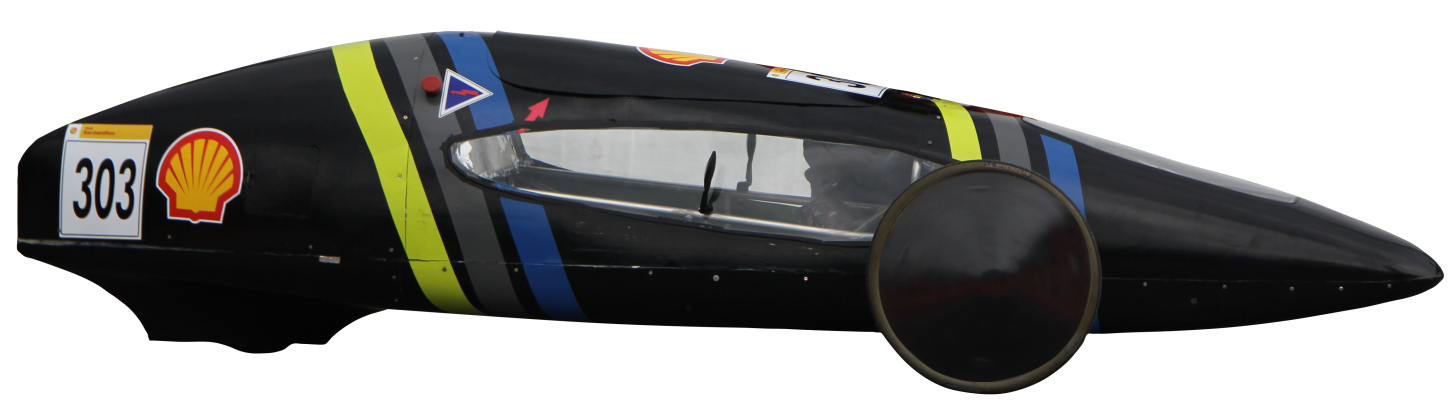
\includegraphics[angle=0, scale=0.8]{1_Introducao/Figuras/dt1.png}
    \caption{Battery electric prototype vehicle DT1}
    \label{fig1}
\end{figure}



\section{METHODOLOGY}

The first step was to define mathematical models of the prototype vehicle DT1 and the track. 
A formulation was then proposed for the optimal control problem (OCP) to find the optimal driving strategy and gear ratio. 
Accordingly, this proposed OPC was solved utilizing MATLAB and the FALCON.m library.

\subsection{Modeling of vehicle dynamics}

A simple model of the vehicle's dynamics was used. 
Only the longitudinal dynamics was modeled. Aerodynamic drag did not consider wind effect. 
Tire rolling resistance was independent of temperature, pressure, or speed. 
Bearing friction was zero. The battery and power converter were treated as ideal. 
The dynamics of the inductor in the motor were disregarded. 
A white-box model was derived by using the fundamental principles that describe the system's behaviour. 
The following equation that describes the longitudinal dynamics was derived from the application of Newton’s second law in the vehicle, as represented in Fig.~\ref{fig:diag_forcas_veiculo}. 

\begin{equation} \label{eq:modelo_1}
	\begin{split}
		\left( m_v + m_p + m_r \right) \ddot x(t) = F_t - (F_a + F_g + F_r) \enspace,\\ 
		m_r = \frac{N_r \cdot J_r + J_m\cdot \varphi^2 }{r_r^2} \enspace,\\ 
		F_{t} =  K_t \cdot i(t) \cdot \eta \cdot \frac{\varphi}{r_r} \enspace,\\
        F_{a} = \frac{\rho \cdot a_f \cdot c_d \cdot {\dot x(t)}^2}{2} \enspace,\\
        F_{g} = (m_v + m_p) \cdot g \cdot \sin(\theta(x)) \enspace,\\
        F_{r}  = c_{r} \cdot (m_v + m_p) \cdot g \cdot \cos(\theta(x)) \enspace,
	\end{split}
\end{equation}


\noindent where $m_v$ is the mass of the vehicle, $m_p$ is the mass of the pilot, $m_r$ is mass equivalent to the moment of inertia of the rotating parts 
(i.e., wheels and engine axle), $x$ is the position, $\varphi$ is the gear ratio, $F_{t}$ is the propulsive force, $i$ is the electric current in the motor, $F_{a}$ is the aerodynamic drag, $F_g$ is the component 
of the weight that is the direction of speed, $F_{r}$ is the rolling resistance of tires on the track, and $\theta$ is the slope of the track. The model constants are shown in Tab. \ref{tab:constantes}.
The experimental validation of this model has not been performed.

\begin{figure}[h]
	\centering
	\begin{normalsize}
		\import{2_Desenvolvimento/Figuras/}{diagrama_forcas_veiculo.pdf_tex}
	\end{normalsize}
	\caption{Diagram of forces of a moving vehicle}
	\label{fig:diag_forcas_veiculo}
\end{figure}

\begin{table}[!h]
	\centering
    \caption{Constants used in the vehicle model}
	\label{tab:constantes}
	% \rowcolors{1}{}{lightgray}
	\begin{tabular}{llll}
		\toprule
		\textbf{Constant} & \textbf{Symbol} & \textbf{Value} & \textbf{Unit}\\
		\midrule
		Vehicle mass                    & $m_v$  & 36               & \si{kg}                \\
        Pilot mass		                & $m_p$  & 50               & \si{kg}                \\  
        Number of wheels                & $N_r$  & 3                & -                      \\
        Moment of inertia of the wheel  & $J_r$  & 0.015            & \si{kg.m^{2}}          \\
        Moment of inertia of the motor  & $J_m$  & \num{0.0625d-3}  & \si{kg.m^{2}}          \\
        Wheel radius                    & $r_r$  & 0.254            & \si{m}                 \\
        Torque constant                 & $K_t$  & 0.119            & \si{N.m / A}           \\
        Transmission efficiency         & $\eta$ & 0.95             & -                      \\
        Air density                     & $\rho$ & 1.22             & \si{kg / m^{3}}        \\
        Frontal area of the vehicle     & $a_f$  & 0.26             & \si{m^{2}}             \\
        Aerodynamic drag coefficient    & $c_d$  & 0.164            & -                      \\
        Gravity acceleration            & $g$    & 9.81             & \si{m / s^{2}}         \\
        Rolling resistance coefficient  & $c_r$  & 0.0024           & -                      \\
		\bottomrule
	\end{tabular}
\end{table}

\subsection{Track modeling}

In 2018 and 2019, SEM Americas was held at the Sonoma Raceway. 
It is expected that the track will remain the same for the next editions of the competition. 
\citet{site:dados_sonoma} made available GPS data collected on the Sonoma Raceway track in 2018. 
This data were used for track modeling. The layout of one lap in Sonoma Raceway is shown in Fig.~\ref{fig:pista}, peaks of elevations are indicated with a triangle, valleys with a square. 

The track’s relative altitude $h$ was approximated by a sum of sines with 8 terms
\footnote{The fit was implemented in MATLAB using the command \lstinline[style=Matlab-editor]{fit(x, h, 'sin8')}}.  
The approximation with trigonometric functions was chosen because of the periodicity of these functions. 
In this way, it would be possible to represent all track laps in a continuous function. 
Using continuous functions instead of interpolating values in tables reduces the computational cost.
The slope model $\theta$ was obtained by deriving the altitude model with respect to $x$:
\[ \theta(x) = arctg\left( \frac{\mathrm{d}h(x)}{\mathrm{d}x}  \right)  \]
\begin{equation}
	\label{eq:modeloTheta}
	\theta(x) = \operatorname{arc\,tan} \left( \sum_{n = 1}^{8} a_n \cdot \cos(b_n \cdot x + c_n) \right)
	\enspace,
\end{equation}

\noindent where the coefficients $a_n$, $b_n$ and $c_n$ are presented in Tab.~\ref{tab:coeficientes}. The fitted curve and the data are displays in Fig.~\ref{fig:altitude_pista}


\begin{figure}[!h]
    \centering
    \begin{minipage}{.5\textwidth}
        \centering
        % This file was created by matlab2tikz.
%
%The latest updates can be retrieved from
%  http://www.mathworks.com/matlabcentral/fileexchange/22022-matlab2tikz-matlab2tikz
%where you can also make suggestions and rate matlab2tikz.
%
%
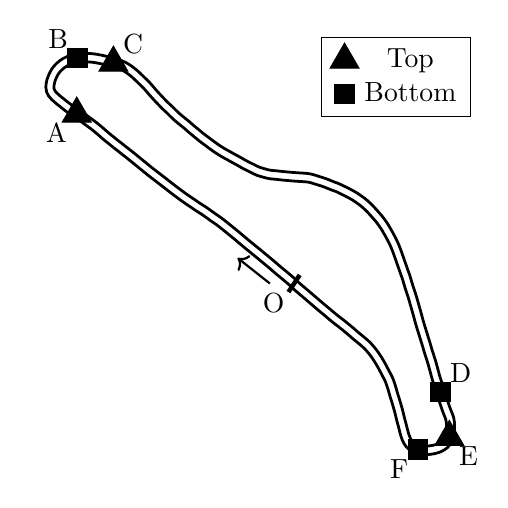
\begin{tikzpicture}

\begin{axis}[%
% width=4.521in,
% height=3.566in,
width=2.2605in,
height=2.26in,
at={(0.758in,2.6in)},
scale only axis,
xmin=-330,
xmax=230,
ymin=-230,
ymax=300,
axis background/.style={fill=white},
axis line style={draw=none},
xtick=\empty, ytick=\empty
]
\addplot [color=black, line width=1pt, forget plot]
  table[row sep=crcr]{%
-4.73238656650697	-2.60902398256989\\
-7.89283938896916	-0.0585958241745614\\
-10.9651059143732	2.41161254599027\\
-14.0610317515681	4.86135937341073\\
-17.1987793236763	7.30667812541416\\
-20.3596019737996	9.77154506542119\\
-23.5075643844916	12.2515498453164\\
-26.7424077140927	14.9230253918275\\
-29.6878625140287	17.346074118677\\
-32.8977313881561	19.8969894998738\\
-35.9745554100071	22.3478798814084\\
-39.0461693558466	24.7406500248347\\
-42.2515954117174	27.2330340332547\\
-45.4676307488345	29.8064148818835\\
-48.4484940144044	32.1283435347169\\
-51.6821193850276	34.5763045056348\\
-54.8349436668391	37.01752287053\\
-57.9654198702129	39.433279596167\\
-61.1878463670267	41.9099306938153\\
-64.4276584524961	44.4815039464233\\
-67.4398138638897	46.8843555357432\\
-70.6671230873407	49.4463357464304\\
-73.7881950060064	51.9583793090802\\
-76.7904582354019	54.2871147715348\\
-80.0525081705761	56.7864468591972\\
-83.2382781086666	59.2814028819272\\
-86.2849115378886	61.5828191781599\\
-89.5663335915205	64.0372807509451\\
-92.7080819519192	66.4455088746133\\
-95.8137128415046	68.7452291628735\\
-98.794079361641	70.7025356920541\\
-102.379021650371	72.9768418706848\\
-105.754283493198	75.2920721976301\\
-108.95813702547	77.482811020808\\
-112.314743509257	79.7415842892376\\
-115.466108795471	81.7643537352265\\
-118.868482986499	83.7975663583247\\
-122.438209019836	85.9661521713886\\
-125.911429360208	88.2035589101987\\
-129.169862746059	90.326210871217\\
-132.498498036343	92.4272441190572\\
-135.998437218732	94.6732913901229\\
-139.353263710683	96.9181131991431\\
-142.714410097924	99.2269583696576\\
-146.033700416929	101.560079799244\\
-149.244503495514	103.826042386363\\
-152.531271526526	106.162001166731\\
-155.857673929233	108.61689189914\\
-158.978573374941	110.927502759444\\
-162.276044609052	113.339748283371\\
-165.491460242591	115.72892687825\\
-168.609229667658	117.99344037314\\
-171.967189227966	120.421178494994\\
-175.154440338945	122.742179308557\\
-178.438124015609	125.145093285276\\
-181.592801342342	127.472809887493\\
-184.949647483525	130.054437174848\\
-187.953627242841	132.389289757053\\
-191.212392214781	134.874994788373\\
-194.34617585508	137.310741355512\\
-197.548811376719	139.812407239064\\
-200.659020878355	142.200411618347\\
-203.91876998839	144.704834413093\\
-206.967783854515	147.032942404613\\
-210.152839329549	149.37088081804\\
-213.415490606613	151.786746064536\\
-216.636084739556	154.206175669978\\
-219.830169868052	156.615865504569\\
-222.865521265795	158.815924537745\\
-226.365938508548	161.425384138848\\
-229.452056274277	163.848439185807\\
-232.535704674991	166.15635995038\\
-235.943147592981	168.78974431836\\
-239.041720345914	171.352754549496\\
-242.090324077265	173.884133533313\\
-245.125475379374	176.323259890661\\
-248.348767077197	178.905632575635\\
-251.176057583704	181.033509301001\\
-254.549923545949	183.419655085213\\
-257.672694086407	185.603530494622\\
-261.056313361613	187.92732419315\\
-264.171221566164	189.987104768033\\
-267.449836678907	191.957123116321\\
-271.084938468976	194.21321151303\\
-274.373797188289	196.355810147903\\
-277.870937190664	198.707262448665\\
-281.171331525877	201.051753450223\\
-284.422066489836	203.361079051739\\
-287.836731937087	205.883425044657\\
-290.951711229744	208.256564640249\\
-294.150421101231	210.657530027144\\
-297.500608389416	213.368105673614\\
-300.483451093876	215.93010902325\\
-304.011158856039	219.827483899135\\
-306.422590444573	224.188268981344\\
-307.550609136123	230.199868599406\\
-307.044071915564	234.902663888923\\
-306.033149891746	239.253168389228\\
-304.318423989251	243.764827698065\\
-302.53963905227	247.429953482638\\
-300.177916028709	251.450128903403\\
-297.209053570142	255.155769515505\\
-293.890050419873	258.342271663906\\
-290.61599050606	260.981195813918\\
-286.649107154644	263.586293234018\\
-282.434954585847	265.559954923848\\
-278.383497135923	267.000712245562\\
-274.35315674267	268.240302141386\\
-269.774555216509	269.222801703332\\
-265.535224713127	269.698651458296\\
-261.273088506036	269.937702071831\\
-257.018626097863	269.918821878033\\
-252.892687411758	269.719565788121\\
-248.670600528564	269.363538578467\\
-244.391017404692	268.7840999477\\
-240.394369886023	268.080199794235\\
-236.43427259268	267.320916798851\\
-232.292101076934	266.413831810356\\
-228.109329677082	265.252333707912\\
-224.392744184788	264.119267284812\\
-220.67822371318	263.088755629493\\
-216.846055860323	262.099575222759\\
-212.771836761231	260.959863150358\\
-208.149494171033	259.033175752892\\
-204.548205520746	256.985770940224\\
-200.898684172864	254.661682817844\\
-197.476365038245	252.217471816168\\
-194.14229121012	249.597718336752\\
-190.94171197296	246.808817036745\\
-187.939216299443	244.041065475051\\
-184.996451278915	241.314713853432\\
-182.073412621385	238.625931845484\\
-179.027487960424	235.7361081165\\
-176.086214693457	232.672159093702\\
-173.383835923788	229.647600393508\\
-170.795770802807	226.794426397805\\
-168.110015552462	223.962443812261\\
-165.359753949486	221.164694020225\\
-162.488754879711	218.295930209478\\
-159.700291547079	215.517001796865\\
-156.928116467472	212.816351340858\\
-154.221922918165	210.407582060605\\
-151.027045043783	207.644137841897\\
-147.968602224376	204.796441253474\\
-145.12304088803	202.117493014745\\
-142.246686477318	199.500539763656\\
-139.468424243858	197.231589771094\\
-136.177648404639	194.726690851998\\
-133.106105969561	192.380905042624\\
-129.876783363463	189.905519397641\\
-126.529532924421	187.07118323573\\
-123.822071535229	184.824429238928\\
-120.584579799111	182.357273249831\\
-117.366668723585	179.820439310081\\
-114.263797116311	177.352676226061\\
-111.188489459749	175.014234741249\\
-108.064685574186	172.78485782333\\
-104.77016658539	170.486039657237\\
-101.491318063615	168.16861077756\\
-98.2563060521595	165.90076637304\\
-94.971519031186	163.642812361349\\
-91.8495227996287	161.636034312079\\
-88.4136463802549	159.545742056473\\
-85.1891176228038	157.68636611086\\
-81.801122895254	155.925428725535\\
-78.0830904567754	153.983835328028\\
-74.6234921721756	152.131923228786\\
-71.1213077993493	150.318363624992\\
-67.5944673386654	148.517936545315\\
-63.8777972343759	146.533575244518\\
-60.4761311486314	144.684104805746\\
-57.0342212475474	142.934462647757\\
-53.5874771366474	141.34005049262\\
-49.7252882864552	139.539659360337\\
-46.18956117614	137.817267656845\\
-42.9083776220702	136.407481725131\\
-39.666369208144	135.385404389109\\
-35.7453336613009	134.372876271339\\
-31.901453071837	133.351848488906\\
-28.6485001228393	132.730369911948\\
-24.9563585983061	132.405640785863\\
-20.7242757138278	132.051977353971\\
-16.6953550148376	131.593077127364\\
-12.8991457162293	131.219233657856\\
-8.87526621671924	130.885361955645\\
-4.87172738754626	130.528998365233\\
-1.01567876995557	130.209806675548\\
2.90126173990634	129.942119451001\\
6.89880130572476	129.705856152961\\
10.9278568816854	129.473851258788\\
14.994738323859	129.196413277665\\
19.3518302682471	128.686143651904\\
23.818567951474	127.704521747567\\
27.7880472537492	126.515441204451\\
31.504163608366	125.389738493466\\
35.3555240690361	124.29768444187\\
39.5056509963823	122.983670355183\\
43.3650238273162	121.544144800964\\
47.0700966544626	120.127377806321\\
50.8892938918558	118.638349413523\\
53.9525037532504	117.664272479604\\
59.0391732705182	115.596254130914\\
61.8956744057682	114.173929277403\\
65.8300476805389	112.452863619829\\
69.5762950783508	110.625961623432\\
73.1359711012941	108.831559150249\\
76.9140402187221	106.791664478392\\
80.5454605431881	104.554735894375\\
83.9250520556913	102.30079358416\\
87.2583720920615	100.017155741827\\
90.7711485830888	97.3532443307433\\
94.0154043357183	94.4972123899162\\
96.9592126426863	91.737649189798\\
99.9666541670764	88.7753955352927\\
102.78460019488	85.7966589705356\\
105.502773758839	82.8788293454264\\
108.292863343777	79.8550249997061\\
111.08113373033	76.5546602700026\\
113.583712260695	73.2405295971062\\
115.93617198821	69.9388347940886\\
118.312470235191	66.2564430394441\\
120.368962055431	62.7868975142443\\
122.423553808867	59.3682978521217\\
124.54756176914	55.6417910360586\\
126.406796611125	52.223139970718\\
128.382509454075	48.2849904214194\\
130.02780146007	44.6049482003815\\
131.654595601188	40.7238373953991\\
133.118239721736	36.9577388882666\\
134.537766572453	33.1594777709772\\
135.918635100333	29.3530573886741\\
137.290699840753	25.6315987868825\\
138.701515317503	21.9069017833792\\
140.104213860124	18.0996011350233\\
141.431994159074	14.4691824933215\\
142.840215052553	10.8375461486692\\
144.311341567293	6.53486722204021\\
145.435927100324	2.82447785162349\\
146.651016366046	-0.931869388917319\\
147.887053313733	-4.71847386169747\\
149.134305296758	-8.26100586570684\\
150.539398785027	-12.199944710644\\
151.817846431873	-16.1205701772408\\
153.005615767889	-20.1058079091772\\
154.093724287177	-23.7166406953759\\
155.317701105057	-27.6730980176675\\
156.452648844799	-31.4965769155037\\
157.590575253269	-35.4120479444184\\
158.677865670897	-39.2811102162789\\
159.762597054294	-43.0300719016368\\
160.9197553921	-46.8068664329385\\
162.127846729139	-50.6022320531358\\
163.3554955285	-54.2477624490664\\
164.667513467389	-58.1855368777564\\
165.887136382035	-62.0133946903123\\
167.116755242715	-65.7430714841902\\
168.398499582795	-69.5665847420466\\
169.634974305547	-73.6223361989428\\
170.725854190368	-77.2392665754502\\
171.948947466435	-80.9050444433333\\
173.244768503186	-84.673565157248\\
174.5603670886	-88.5321103594271\\
175.816382818875	-92.5037613231765\\
176.948574008273	-96.3316268468371\\
178.07516578893	-100.230550783254\\
179.150869513685	-104.13758219127\\
180.212023801598	-107.915855804586\\
181.353500815093	-111.471759958763\\
182.669133238087	-115.181617800726\\
183.995557652315	-119.244605405915\\
185.145004777531	-123.03501174266\\
186.337025820032	-126.958887548448\\
187.481187053129	-130.22452759345\\
188.990771050589	-134.16147381027\\
190.35106221487	-137.966547382178\\
191.672079392948	-141.757415066363\\
192.975110880458	-145.381383332428\\
194.384442548563	-148.88835406649\\
195.953144042691	-152.425855078302\\
197.591343632798	-156.89872843854\\
198.497410353015	-161.634988090118\\
198.798391394146	-166.044972521666\\
198.754637665533	-170.414136729587\\
198.437602771983	-174.683800615099\\
197.65957013364	-179.249426081656\\
196.081091312305	-183.902598514296\\
193.868209146235	-188.029833335734\\
190.310042910658	-192.135892761611\\
186.284260385131	-195.011667173174\\
182.206223148917	-197.070739705986\\
177.886441912141	-198.612319859321\\
173.414206177984	-199.620280751486\\
169.297882493636	-200.241667246531\\
164.91043559313	-200.641789597692\\
160.542793900447	-200.69583938203\\
155.832824254913	-200.227226235001\\
151.35902848966	-199.160029930101\\
146.856776602027	-197.364153495651\\
142.78212102211	-194.920390815717\\
138.952785976461	-191.478727591967\\
136.105861421973	-187.66260176603\\
133.873510626759	-183.198891756612\\
132.46456823375	-179.316023477929\\
131.182967107325	-175.149088085413\\
130.146687145805	-171.14882425582\\
129.16316582771	-167.458161146447\\
128.073632013942	-163.668770371653\\
126.969372068832	-159.708197232558\\
125.938647602133	-155.716481577071\\
124.97155615596	-151.885394069675\\
123.941237197623	-148.316143263819\\
122.730626161416	-144.415299319114\\
121.583689687623	-140.6056259504\\
120.40572074922	-137.042208928714\\
119.067892370229	-133.110999571277\\
117.87211322586	-129.158400583473\\
116.776719402138	-125.427440790027\\
115.601762315197	-121.789985537147\\
114.292931524982	-118.067331645023\\
112.938608465798	-114.737755844022\\
111.328379020242	-111.594457037056\\
109.328711471661	-108.056742062542\\
107.367001480716	-104.552952327915\\
105.400977002647	-100.993831937512\\
103.514026263549	-97.7126798218527\\
101.445932972948	-94.3342559801604\\
99.3927737397856	-91.1862693406631\\
97.141753124057	-87.9255507744207\\
94.9680224668095	-84.9920541008122\\
92.5590143690601	-82.0877697979861\\
89.9782073771724	-79.1687202617677\\
87.4324774086506	-76.5280250617184\\
84.7773262422367	-74.1688856482907\\
81.6679828885499	-71.6276936783907\\
78.6653074147493	-69.2475702873308\\
75.5182532291431	-66.8851409901199\\
72.1590650075697	-64.2270229837538\\
69.1178041928673	-61.6766308196025\\
66.0855540622897	-59.1843113010962\\
63.0413873534316	-56.7847403209303\\
59.8419589466482	-54.3112949811606\\
56.711932608885	-51.893701352171\\
53.6416518710089	-49.6371650660026\\
50.3649777999799	-47.3061615955092\\
46.9800337570735	-44.7492215429701\\
43.8611248336124	-42.3050806152286\\
40.6047665167058	-39.7099104953934\\
37.5449492214464	-37.2011309316973\\
34.5833412278778	-34.902004727165\\
30.406442744474	-31.6441910615212\\
27.195878225692	-29.0403898057287\\
24.6776467349898	-26.9907014491863\\
21.668728553742	-24.5469747312195\\
18.8175080510238	-22.2505008420462\\
15.7028529013626	-19.7278447637192\\
12.6046209458534	-17.1919483131002\\
9.52120702031128	-14.7126582600479\\
6.36063004520681	-12.2130128305592\\
3.18109748715986	-9.63899967540168\\
0.114082434129711	-7.13623944708169\\
-4.73238656650697	-2.60902398256989\\
};
\addplot [color=black, line width=1pt, forget plot]
  table[row sep=crcr]{%
1.53880524038682	5.18020918386878\\
-1.60376882250141	7.71620908720354\\
-4.72234695245479	10.2236520071929\\
-7.8926318312805	12.7322451192081\\
-11.0736749257357	15.2113031079373\\
-14.1860667646708	17.6384035884689\\
-17.3043039520425	20.094990417362\\
-20.2129611828268	22.4970816363599\\
-23.5091587278328	25.2088738441213\\
-26.632083520547	27.6906828989706\\
-29.7793771155531	30.1977057329751\\
-32.9511580152136	32.6685019884852\\
-36.0715036092345	35.0947428368726\\
-39.1514382023042	37.5592022332273\\
-42.4770584139974	40.1496873666562\\
-45.5814635912246	42.4998137588343\\
-48.6912963227732	44.9077444968058\\
-51.8900789988428	47.3762156588997\\
-55.0757821143021	49.8246429798409\\
-58.103872865773	52.2280990599653\\
-61.2912584569447	54.7707530915178\\
-64.3826750928959	57.2248776024031\\
-67.5330001083875	59.7604647221479\\
-70.7898622718837	62.2866677642095\\
-73.892100298009	64.6635894149477\\
-77.0671079965627	67.1501168459417\\
-80.4040359061352	69.6707918415563\\
-83.4676113358817	71.9622783439148\\
-86.6393056858445	74.3934617325716\\
-89.9820779031658	76.8687772759794\\
-93.6604487492843	79.2842509481014\\
-96.8043529482077	81.2788337317453\\
-100.015956662378	83.4817977841616\\
-103.407729294034	85.8010424443025\\
-106.699329345061	88.0160706034776\\
-110.282054772334	90.3157035634813\\
-113.792553387588	92.4135363389419\\
-117.130437851709	94.4412666382729\\
-120.387793642851	96.5395920472451\\
-123.777553309251	98.7477902324599\\
-127.214544218609	100.917228338834\\
-130.480227106461	103.012917110551\\
-133.749041899549	105.200184068896\\
-136.995754091367	107.430431626679\\
-140.251015203165	109.718544833705\\
-143.495574369124	112.008328979959\\
-146.695713122385	114.282731313205\\
-149.815896832201	116.585387962375\\
-153.118792884078	119.030772013202\\
-156.327494930116	121.378078751647\\
-159.511332382137	123.743792489889\\
-162.83488093387	126.157807874704\\
-166.0251547927	128.464326309756\\
-169.324787249084	130.867149760926\\
-172.457873608933	133.159867460101\\
-175.698929323095	135.551316718631\\
-178.6571832443	137.826495705126\\
-181.975309206598	140.405505413928\\
-185.061432674267	142.759517394781\\
-188.223455148624	145.217212828345\\
-191.3604403085	147.667600649925\\
-194.668722046316	150.207678311974\\
-197.722295149589	152.553636842261\\
-201.023407498852	155.074359552245\\
-204.263846321873	157.452944994694\\
-207.405652261171	159.779357844278\\
-210.633330361935	162.204109145693\\
-213.787609212682	164.583767406964\\
-217.172484452447	167.037197665543\\
-220.118576986282	169.233743378158\\
-223.351008386952	171.771646533628\\
-226.652515444692	174.242649858644\\
-229.602176006617	176.522278142464\\
-232.634591205714	179.030559976881\\
-235.720476116877	181.592897180069\\
-238.968795456518	184.203316510223\\
-242.000927268183	186.632529090996\\
-245.51319536133	189.275595896664\\
-248.66818525022	191.507000423491\\
-252.09880469926	193.906045601495\\
-255.310639891093	196.111897265105\\
-258.894598012521	198.481646772941\\
-262.427031750467	200.604170626936\\
-265.567916719034	202.553623433953\\
-268.974410785961	204.77285395665\\
-272.114773554243	206.8844612472\\
-275.344951909589	209.179071615946\\
-278.665098141517	211.537711331379\\
-281.709128467927	213.786112924406\\
-284.958185391327	216.261416170679\\
-288.137527929229	218.647843894701\\
-290.944534176962	220.919124871099\\
-294.008449600591	223.55076225391\\
-295.786064730379	225.514998877052\\
-297.235654084651	228.137977871724\\
-297.556857228849	229.84642438054\\
-297.204249335829	233.119999703121\\
-296.418321363245	236.504519199622\\
-295.293332966004	239.458119904158\\
-293.573389040895	243.00204644505\\
-291.940377244414	245.780653197728\\
-289.866388799246	248.367155955856\\
-287.427454722042	250.711095028132\\
-284.524695957211	253.050487729569\\
-281.799480270228	254.840944808601\\
-278.823794430332	256.234745954006\\
-275.28932158863	257.491449514806\\
-271.570741029079	258.63519085641\\
-268.384675559286	259.31986100178\\
-264.687608870167	259.734638843754\\
-261.011618372819	259.941120987809\\
-257.361274934765	259.924694013403\\
-253.515816285794	259.738999150583\\
-249.722695248665	259.41903775138\\
-246.027389195124	258.918894052054\\
-242.227928864702	258.249733809771\\
-238.365627172018	257.509195773013\\
-234.638077667735	256.692906245606\\
-231.115890106631	255.715007332902\\
-227.218660103849	254.526864081318\\
-223.200173947828	253.41199134519\\
-219.322112540441	252.410966276329\\
-215.673834998093	251.390202433632\\
-212.934765425649	250.252448048439\\
-209.642639291165	248.38072912982\\
-206.542476356403	246.406526260332\\
-203.45348919763	244.20036593042\\
-200.519889570689	241.89536550458\\
-197.696428605328	239.434957584843\\
-194.739738210358	236.709428431446\\
-191.788165672562	233.974917153582\\
-188.822119823231	231.246572042374\\
-186.043810488841	228.610715623646\\
-183.493871873026	225.954524457167\\
-180.889077347948	223.039170083285\\
-178.101607886034	219.966194964019\\
-175.315420562925	217.02831527039\\
-172.418460735895	214.081286753696\\
-169.566866418322	211.231913147849\\
-166.739647440012	208.414363652301\\
-163.845304905514	205.594682273903\\
-160.594017664486	202.700675512325\\
-157.735009338509	200.227722601319\\
-154.886797918401	197.575737109198\\
-151.911584128186	194.774763231039\\
-148.918079371621	192.051209803866\\
-145.442623234752	189.212303866651\\
-142.318420092963	186.834230964746\\
-139.102929501937	184.378523676959\\
-136.045216060312	182.034659338889\\
-133.273696015016	179.687670236658\\
-129.829079361931	176.829689907972\\
-126.698897355856	174.444301569402\\
-123.635017723897	172.028918225576\\
-120.445578476844	169.492295878357\\
-117.107629588609	166.954223566634\\
-113.762081799793	164.566605195889\\
-110.517134785293	162.302375654524\\
-107.288063638834	160.020129892378\\
-103.941536483053	157.674092990217\\
-100.614983039135	155.387431450029\\
-97.0222199140444	153.077809930672\\
-93.6364138019737	151.017981479473\\
-89.958627882955	148.89706739718\\
-86.2514983372227	146.970309607091\\
-82.8866730384783	145.213111618963\\
-79.2581536044872	143.270776948093\\
-75.6827323999285	141.419295942744\\
-72.1267053509604	139.603968932635\\
-68.7622593833998	137.807635208352\\
-65.1424002833055	135.839562287176\\
-61.4330762162247	133.953923968783\\
-57.5795968991282	132.171463916598\\
-54.1783673223158	130.585884340806\\
-50.4944927694071	128.791329258136\\
-46.4859593119715	127.069339016215\\
-42.1122307544345	125.689128748618\\
-38.301842816292	124.705184667836\\
-34.4791506104544	123.689784765281\\
-29.8253991231069	122.799865959823\\
-25.5231940931225	122.421718834956\\
-21.8205233853027	122.112246922879\\
-17.8621078564046	121.661375973649\\
-13.6885076344571	121.250436952032\\
-9.73907135850419	120.922739776869\\
-5.78156331257404	120.570474449033\\
-1.75543884158686	120.23720646114\\
2.27639911213911	119.961661210198\\
6.34332068028444	119.721296008681\\
10.3331547012664	119.491550456037\\
14.2290749278936	119.225768385579\\
17.7892141284059	118.808986631814\\
21.1012421645145	118.080793750189\\
24.7650525075629	116.98331118202\\
28.7260469602411	115.783382894728\\
32.6779979117653	114.662807500408\\
36.141886726731	113.566394212996\\
39.7422903217836	112.223425840074\\
43.5495799778076	110.767572128349\\
47.1428405150543	109.36666741426\\
51.63581421225	107.936325647378\\
53.9107776996847	107.011409410766\\
58.1547538275009	104.900013533387\\
61.5679984827208	103.406597172538\\
65.0694667465757	101.69912016702\\
68.6400749078468	99.8992068610841\\
71.9116681569224	98.132780384277\\
75.0599904828498	96.1935387183041\\
78.3146677303037	94.022896041822\\
81.5647906028749	91.796259815835\\
84.3935816921704	89.6508654416039\\
87.1859214837128	87.192545116579\\
90.1104491313156	84.4510561336903\\
92.7838018922779	81.8179079716372\\
95.4398295610275	79.0103238523669\\
98.213162931779	76.0332779439675\\
100.883034273734	73.1397861243758\\
103.221703461198	70.3716710378716\\
105.485000046653	67.3744525029897\\
107.747683298312	64.1987430722251\\
109.70784462472	61.1613063284599\\
111.768722339047	57.6843612017091\\
113.882333381306	54.1675715943942\\
115.719703212774	50.9440348366812\\
117.66585343494	47.3655775788691\\
119.264164206329	44.1794112974812\\
120.887917467079	40.5475450167354\\
122.353142121081	37.0519219337622\\
123.778197801202	33.3851184322611\\
125.143959536681	29.7307186113569\\
126.511576065585	25.960825038619\\
127.933571226651	22.103972942332\\
129.355377283091	18.3502595689129\\
130.68364047314	14.7450822335327\\
132.069296854555	10.9563632289759\\
133.556805463848	7.12024788133158\\
134.697462167363	3.78290012856109\\
135.912981715696	-0.227326729503651\\
137.144917204308	-4.03575062491969\\
138.380445990106	-7.82079834413869\\
139.781793324182	-11.8008532921963\\
141.058604918742	-15.3802823758941\\
142.285035893183	-19.141418275614\\
143.372530233991	-22.7897719731352\\
144.578968063611	-26.7938819933772\\
145.726664125274	-30.5036473729058\\
146.870493398278	-34.3570483799146\\
147.967526323719	-38.1317775816205\\
149.04683885856	-41.9724523610151\\
150.183048166529	-45.8992604815181\\
151.376539763714	-49.7946809302135\\
152.61375201822	-53.681517981996\\
153.91729308959	-57.5523554228162\\
155.134716570264	-61.2064280241185\\
156.363910444123	-65.0643236857955\\
157.646209930595	-68.9537990483253\\
158.906182734025	-72.7123629990993\\
160.002845636209	-76.3097322057324\\
161.215308035441	-80.3294950192736\\
162.488363744129	-84.145006732193\\
163.79211192534	-87.936582720991\\
165.083098239435	-91.7229370799886\\
166.226836836367	-95.3393578828711\\
167.359437598871	-99.1686081513022\\
168.450314325634	-102.943894533959\\
169.49392280034	-106.73438410432\\
170.615183308188	-110.726665749077\\
171.915536231095	-114.777032188276\\
173.25732991316	-118.560664733352\\
174.402537607733	-122.06842665101\\
175.598526525648	-126.012385247332\\
176.746684969194	-129.791794600355\\
178.217893249766	-133.991673451068\\
179.584853866715	-137.556870978513\\
180.924077819311	-141.30300736334\\
182.213183746578	-145.002302298778\\
183.614931492975	-148.900906287908\\
185.192582316773	-152.826590407701\\
186.863268792277	-156.594088268986\\
187.957898899327	-159.5814029561\\
188.555945254179	-162.715391574297\\
188.80204032973	-166.315093599979\\
188.765359338433	-169.951191264412\\
188.490132636242	-173.66016107965\\
187.932699705821	-176.928221290945\\
186.950475505441	-179.824381380859\\
185.422982036351	-182.674635947916\\
183.778885822933	-184.563311491301\\
181.250940794492	-186.370735863501\\
178.249372271593	-187.88687716702\\
175.130194310456	-188.99966678339\\
171.769062782329	-189.756533836254\\
167.962612651512	-190.331215468297\\
164.423772379043	-190.653638671917\\
160.784483009008	-190.698760489933\\
157.564629144774	-190.378325188516\\
154.257574237869	-189.589322926669\\
151.343545613613	-188.42721308874\\
148.548786036026	-186.750594330046\\
146.474498220396	-184.889050443621\\
144.558875152623	-182.319703781842\\
143.222343567227	-179.649339298735\\
141.914276001485	-176.044475968811\\
140.836443557396	-172.539415227003\\
139.853337790702	-168.744467115558\\
138.778915138867	-164.712734916334\\
137.67904622057	-160.887400579785\\
136.627206892543	-157.114700265543\\
135.64556472837	-153.313200506459\\
134.656382428807	-149.394582943804\\
133.46224852404	-145.258310154863\\
132.309937490968	-141.545317707408\\
131.155302964938	-137.710074315645\\
129.817859745511	-133.664097101897\\
128.587694451238	-130.049403853612\\
127.492427007873	-126.429011872494\\
126.345854685303	-122.523710442268\\
125.061499071606	-118.547551189401\\
123.700681810542	-114.677016827112\\
122.038305205874	-110.591007812294\\
120.013099377163	-106.637075437656\\
118.054818171431	-103.172577664794\\
116.091886141996	-99.6666052621236\\
114.182350452259	-96.2097457825133\\
112.065789573388	-92.5293079181114\\
109.951590231645	-89.0755684445135\\
107.634912064814	-85.5234824092047\\
105.358347915696	-82.2257639336679\\
102.813443865178	-78.7912990595276\\
100.105936428805	-75.526979645563\\
97.4124816873339	-72.4805541841892\\
94.400001575561	-69.354908097419\\
91.0640082447297	-66.3921492248589\\
88.0367314212415	-63.9180216926744\\
84.7204991738896	-61.2892631331654\\
81.4680223753724	-58.8477130988988\\
78.6099738824331	-56.5859645041838\\
75.5181342123351	-53.9931566287237\\
72.383985367362	-51.4170876597115\\
69.1250392087753	-48.8481680064501\\
65.9915612419688	-46.425713733758\\
62.7886851976016	-43.9518452734243\\
59.4033726587384	-41.4638809302194\\
56.1964132744849	-39.1824702974179\\
53.1993883276792	-36.9185364691668\\
49.9783983849569	-34.3943939005356\\
46.952703730116	-31.9830940012218\\
43.8777066262369	-29.461868457012\\
40.5169554655865	-26.8526431327241\\
36.7010807330964	-23.873892959634\\
33.5069126606405	-21.2834029963488\\
30.9911042028141	-19.2356866328256\\
27.9616294114469	-16.7752697191196\\
25.0724369216309	-14.4482021536053\\
22.0347761805729	-11.9878998294064\\
18.9403816036832	-9.45514426448324\\
15.718994089106	-6.86489198868881\\
12.5695151602992	-4.37402401645922\\
9.5546798488069	-1.93332333394392\\
6.38526377811117	0.653002143143822\\
1.53880524038682	5.18020918386878\\
};
\addplot [mark=triangle*,
      only marks,
      mark size=6pt]
  table[row sep=crcr]{%
  -269.2	199\\
  -223.8	258.7\\
  192.3	-180.1\\
};
\addlegendentry{Top}

\addplot[mark=square*,
        only marks,
        mark size=3.5pt]   
    table[row sep=crcr]{%
    -268.1	264.4\\
    181.3	-127.5\\
    153.5	-194.6\\
};
\addlegendentry{Bottom}
% \draw[
%   help lines,
%   line width=0.1pt,
%   blue
% ] (-100, -100) grid[step={($(10, 10) - (0, 0)$)}] (100, 100);

\draw[ultra thick] (-7,-10) -- (0,0) -- (7,10);
\draw[thick, ->] (-30,0) -- (-70,30);

\filldraw[black] (0,	0) circle (0pt) node[anchor= north east] {O};
\filldraw[black] (-269.2,	199) circle (0pt) node[anchor= north east] {A};
\filldraw[black] (-268.1,	264.4) circle (0pt) node[anchor= south east] {B};
\filldraw[black] (-223.8,	258.7) circle (0pt) node[anchor= south west] {C};
\filldraw[black] (181.3,-127.5) circle (0pt) node[anchor= south west] {D};
\filldraw[black] (192.3,-180.1) circle (0pt) node[anchor= north west] {E};
\filldraw[black] (153.5,	-194.6) circle (0pt) node[anchor= north east] {F};

\end{axis}

\end{tikzpicture}%
        \caption{Layout of the racing track in Sonoma}
        \label{fig:pista}
    \end{minipage}%
    \begin{minipage}{.5\textwidth}
        \centering

        % This file was created by matlab2tikz.
%
%The latest updates can be retrieved from
%  http://www.mathworks.com/matlabcentral/fileexchange/22022-matlab2tikz-matlab2tikz
%where you can also make suggestions and rate matlab2tikz.
%
\definecolor{mycolor1}{rgb}{0.00000,0.44700,0.74100}%
\definecolor{mycolor2}{rgb}{0.85000,0.32500,0.09800}%
%
\begin{tikzpicture}[scale=1][]

  \begin{axis}[%
    width=2.7in,
    height=1.783in,
    at={(0.758in,2.6in)},
    scale only axis,
    xmin=0,
    xmax=1440,
    ymin=-2.5,
    ymax=6,
    ylabel style={font=\color{white!15!black}},
    ylabel={Relative altitude (\si{m})},
    xlabel={Distance along track (\si{m})},
    axis background/.style={fill=white},
    xmajorgrids,
    ymajorgrids,
    %xtick={0,350,700,1050,1440},
    xtick={0,400,800,1200,1440},
    clip marker paths=true,
    legend style={legend cell align=left, align=left, draw=white!15!black}
    ]
    \addplot [color=mycolor2, only marks, mark=o, mark options={solid, mycolor2}]
      table[row sep=crcr]{%
    0	0\\
    5.1222	0.035738\\
    10.052	0.10497\\
    15.102	0.10772\\
    20.056	0.14341\\
    25.018	0.18539\\
    30.099	0.24281\\
    35.019	0.26534\\
    40.103	0.30621\\
    45.03	0.34432\\
    50.02	0.36324\\
    55.06	0.4084\\
    60.082	0.44874\\
    65.003	0.50745\\
    70.013	0.52866\\
    75.043	0.54874\\
    80.029	0.58008\\
    85.054	0.60309\\
    90.004	0.64756\\
    95.034	0.69913\\
    100.08	0.73437\\
    105.09	0.77665\\
    110.03	0.80147\\
    115.11	0.8308\\
    120.05	0.85947\\
    125.08	0.91471\\
    130.04	0.987\\
    135.06	1.0446\\
    140.02	1.1265\\
    145.07	1.1976\\
    150.07	1.2977\\
    155.07	1.4261\\
    160.05	1.5534\\
    165.02	1.7003\\
    170.06	1.8176\\
    175.03	1.8384\\
    180.1	1.8899\\
    185.09	1.959\\
    190.08	2.0057\\
    195.07	2.0065\\
    200.08	2.1076\\
    205.05	2.2171\\
    210.04	2.3643\\
    215.1	2.5291\\
    220.07	2.6873\\
    225.1	2.8419\\
    230.05	3.0317\\
    235.08	3.1583\\
    240.02	3.2784\\
    245.01	3.4202\\
    250.02	3.5219\\
    255.05	3.6083\\
    260.01	3.6875\\
    265	3.8082\\
    270.07	3.9549\\
    275.02	4.0884\\
    280.08	4.2276\\
    285.07	4.3234\\
    290.09	4.4291\\
    295.02	4.4829\\
    300.06	4.5449\\
    305.07	4.61\\
    310.07	4.648\\
    315.05	4.6728\\
    320.01	4.6917\\
    325.05	4.7362\\
    330.01	4.7312\\
    335.08	4.7492\\
    340.01	4.7603\\
    345.05	4.7026\\
    350.06	4.6628\\
    355.04	4.5688\\
    360.09	4.3908\\
    365.05	4.1747\\
    370.01	3.9563\\
    375.05	3.7561\\
    380.01	3.5984\\
    385.01	3.5353\\
    390.02	3.4615\\
    395.07	3.4505\\
    400.1	3.4657\\
    405.04	3.5032\\
    410.05	3.4511\\
    415	3.3952\\
    420.07	3.3656\\
    425.01	3.2732\\
    430.02	3.1978\\
    435.03	3.1787\\
    440.06	3.3637\\
    445.07	3.6768\\
    450.11	4.0237\\
    455.11	4.3273\\
    460.03	4.5621\\
    465.01	4.7456\\
    470.09	4.8381\\
    475.01	4.8199\\
    480.09	4.8295\\
    485	4.8346\\
    490.09	4.8057\\
    495.09	4.7223\\
    500.09	4.6332\\
    505.1	4.5413\\
    510.02	4.4621\\
    515.05	4.3114\\
    520.05	4.2162\\
    525.01	4.134\\
    530.04	4.0624\\
    535.01	3.9909\\
    540	3.9346\\
    545.08	3.8595\\
    550.12	3.8051\\
    555.1	3.7335\\
    560.09	3.6563\\
    565.02	3.599\\
    570.06	3.5572\\
    575.09	3.5131\\
    580.08	3.4391\\
    585	3.3567\\
    590.01	3.2757\\
    595.05	3.2379\\
    600.02	3.1674\\
    605.08	3.0848\\
    610.02	2.9922\\
    615	2.9465\\
    620.02	2.8593\\
    625.11	2.7651\\
    630.08	2.6997\\
    635.08	2.6199\\
    640.02	2.5204\\
    645.04	2.4145\\
    650.07	2.3246\\
    655	2.2181\\
    660.06	2.1146\\
    665.02	2.038\\
    670.06	1.9449\\
    675.05	1.8925\\
    680.09	1.8092\\
    685.08	1.709\\
    690.04	1.6652\\
    695.04	1.5816\\
    700.02	1.4836\\
    705.1	1.4271\\
    710.02	1.3237\\
    715	1.2147\\
    720.11	1.1747\\
    725.08	1.0693\\
    730.02	0.9783\\
    735.02	0.87326\\
    740.01	0.80079\\
    745.06	0.67547\\
    750.09	0.61633\\
    755.06	0.53173\\
    760.08	0.42591\\
    765	0.38467\\
    770.1	0.25097\\
    775.04	0.185\\
    780.1	0.094467\\
    785.11	0.0042468\\
    790.01	-0.087749\\
    795.03	-0.15127\\
    800.04	-0.19791\\
    805.06	-0.29861\\
    810.07	-0.35415\\
    815.01	-0.43642\\
    820.07	-0.50071\\
    825.05	-0.5167\\
    830.08	-0.56259\\
    835.08	-0.6105\\
    840.01	-0.64431\\
    845.08	-0.66497\\
    850.11	-0.67766\\
    855.07	-0.70386\\
    860.02	-0.69959\\
    865.1	-0.70008\\
    870.02	-0.72612\\
    875.09	-0.75503\\
    880.11	-0.74512\\
    885.04	-0.72702\\
    890.06	-0.72219\\
    895.01	-0.74177\\
    900.04	-0.74645\\
    905.09	-0.78183\\
    910.06	-0.79228\\
    915.01	-0.79059\\
    920.11	-0.80498\\
    925	-0.81388\\
    930.09	-0.82108\\
    935.08	-0.85434\\
    940.08	-0.87037\\
    945.02	-0.8898\\
    950.11	-0.91711\\
    955	-0.941\\
    960.02	-0.95908\\
    965.01	-0.97259\\
    970.07	-0.9977\\
    975.02	-1.0021\\
    980.02	-1.0205\\
    985.06	-1.03\\
    990.07	-1.0475\\
    995.09	-1.0488\\
    1000.1	-1.0607\\
    1005	-1.0603\\
    1010.1	-1.0762\\
    1015	-1.0899\\
    1020.1	-1.0865\\
    1025	-1.1233\\
    1030	-1.1057\\
    1035.1	-1.1309\\
    1040.1	-1.1516\\
    1045.1	-1.1333\\
    1050.1	-1.1306\\
    1055	-1.1343\\
    1060.1	-1.1496\\
    1065	-1.2185\\
    1070.1	-1.294\\
    1075.1	-1.3496\\
    1080.1	-1.4133\\
    1085.1	-1.4789\\
    1090.1	-1.4778\\
    1095.1	-1.4619\\
    1100	-1.4065\\
    1105	-1.3362\\
    1110.1	-1.2712\\
    1115.1	-1.2374\\
    1120.1	-1.1685\\
    1125.1	-1.0986\\
    1130	-1.0041\\
    1135	-0.92332\\
    1140	-0.88023\\
    1145.1	-0.91493\\
    1150.1	-0.9995\\
    1155	-1.0491\\
    1160.1	-1.1572\\
    1165	-1.2352\\
    1170.1	-1.2925\\
    1175	-1.2543\\
    1180.1	-1.2889\\
    1185.1	-1.2424\\
    1190.1	-1.2007\\
    1195	-1.1524\\
    1200.1	-1.0711\\
    1205	-1.0818\\
    1210	-1.0683\\
    1215.1	-1.0743\\
    1220	-1.0607\\
    1225	-1.0466\\
    1230.1	-1.0469\\
    1235.1	-1.049\\
    1240	-1.0506\\
    1245	-1.0674\\
    1250	-1.0704\\
    1255.1	-1.0248\\
    1260.1	-1.0326\\
    1265	-1.0105\\
    1270.1	-0.99422\\
    1275	-0.98019\\
    1280.1	-0.93839\\
    1285	-0.93409\\
    1290.1	-0.92035\\
    1295.1	-0.9174\\
    1300	-0.93492\\
    1305.1	-0.91239\\
    1310.1	-0.89661\\
    1315.1	-0.85047\\
    1320.1	-0.81659\\
    1325.1	-0.76624\\
    1330.1	-0.78241\\
    1335	-0.77116\\
    1340.1	-0.73442\\
    1345.1	-0.71422\\
    1350	-0.70423\\
    1355	-0.66556\\
    1360.1	-0.63987\\
    1365.1	-0.60605\\
    1370	-0.59789\\
    1375	-0.54782\\
    1380	-0.49583\\
    1385	-0.46034\\
    1390	-0.41838\\
    1395.1	-0.363\\
    1401.9	-0.32049\\
    1406.3	-0.28726\\
    1410.6	-0.25818\\
    1415.1	-0.22964\\
    1420	-0.17512\\
    1425	-0.12472\\
    1430.1	-0.10287\\
    1435.1	-0.048184\\
    1440	-0.01308\\
    1440	0\\
    1445.1222	0.035738\\
    1450.052	0.10497\\
    1455.102	0.10772\\
    1460.056	0.14341\\
    1465.018	0.18539\\
    1470.099	0.24281\\
    1475.019	0.26534\\
    1480.103	0.30621\\
    1485.03	0.34432\\
    1490.02	0.36324\\
    1495.06	0.4084\\
    1500.082	0.44874\\
    1505.003	0.50745\\
    1510.013	0.52866\\
    1515.043	0.54874\\
    1520.029	0.58008\\
    1525.054	0.60309\\
    1530.004	0.64756\\
    1535.034	0.69913\\
    1540.08	0.73437\\
    1545.09	0.77665\\
    1550.03	0.80147\\
    1555.11	0.8308\\
    1560.05	0.85947\\
    1565.08	0.91471\\
    1570.04	0.987\\
    1575.06	1.0446\\
    1580.02	1.1265\\
    1585.07	1.1976\\
    1590.07	1.2977\\
    1595.07	1.4261\\
    1600.05	1.5534\\
    1605.02	1.7003\\
    1610.06	1.8176\\
    1615.03	1.8384\\
    1620.1	1.8899\\
    1625.09	1.959\\
    1630.08	2.0057\\
    1635.07	2.0065\\
    1640.08	2.1076\\
    1645.05	2.2171\\
    1650.04	2.3643\\
    1655.1	2.5291\\
    1660.07	2.6873\\
    1665.1	2.8419\\
    1670.05	3.0317\\
    1675.08	3.1583\\
    1680.02	3.2784\\
    1685.01	3.4202\\
    1690.02	3.5219\\
    1695.05	3.6083\\
    1700.01	3.6875\\
    1705	3.8082\\
    1710.07	3.9549\\
    1715.02	4.0884\\
    1720.08	4.2276\\
    1725.07	4.3234\\
    1730.09	4.4291\\
    1735.02	4.4829\\
    1740.06	4.5449\\
    1745.07	4.61\\
    1750.07	4.648\\
    1755.05	4.6728\\
    1760.01	4.6917\\
    1765.05	4.7362\\
    1770.01	4.7312\\
    1775.08	4.7492\\
    1780.01	4.7603\\
    1785.05	4.7026\\
    1790.06	4.6628\\
    1795.04	4.5688\\
    1800.09	4.3908\\
    1805.05	4.1747\\
    1810.01	3.9563\\
    1815.05	3.7561\\
    1820.01	3.5984\\
    1825.01	3.5353\\
    1830.02	3.4615\\
    1835.07	3.4505\\
    1840.1	3.4657\\
    1845.04	3.5032\\
    1850.05	3.4511\\
    1855	3.3952\\
    1860.07	3.3656\\
    1865.01	3.2732\\
    1870.02	3.1978\\
    1875.03	3.1787\\
    1880.06	3.3637\\
    1885.07	3.6768\\
    1890.11	4.0237\\
    1895.11	4.3273\\
    1900.03	4.5621\\
    1905.01	4.7456\\
    1910.09	4.8381\\
    1915.01	4.8199\\
    1920.09	4.8295\\
    1925	4.8346\\
    1930.09	4.8057\\
    1935.09	4.7223\\
    1940.09	4.6332\\
    1945.1	4.5413\\
    1950.02	4.4621\\
    1955.05	4.3114\\
    1960.05	4.2162\\
    1965.01	4.134\\
    1970.04	4.0624\\
    1975.01	3.9909\\
    1980	3.9346\\
    1985.08	3.8595\\
    1990.12	3.8051\\
    1995.1	3.7335\\
    2000.09	3.6563\\
    2005.02	3.599\\
    2010.06	3.5572\\
    2015.09	3.5131\\
    2020.08	3.4391\\
    2025	3.3567\\
    2030.01	3.2757\\
    2035.05	3.2379\\
    2040.02	3.1674\\
    2045.08	3.0848\\
    2050.02	2.9922\\
    2055	2.9465\\
    2060.02	2.8593\\
    2065.11	2.7651\\
    2070.08	2.6997\\
    2075.08	2.6199\\
    2080.02	2.5204\\
    2085.04	2.4145\\
    2090.07	2.3246\\
    2095	2.2181\\
    2100.06	2.1146\\
    2105.02	2.038\\
    2110.06	1.9449\\
    2115.05	1.8925\\
    2120.09	1.8092\\
    2125.08	1.709\\
    2130.04	1.6652\\
    2135.04	1.5816\\
    2140.02	1.4836\\
    2145.1	1.4271\\
    2150.02	1.3237\\
    2155	1.2147\\
    2160.11	1.1747\\
    2165.08	1.0693\\
    2170.02	0.9783\\
    2175.02	0.87326\\
    2180.01	0.80079\\
    2185.06	0.67547\\
    2190.09	0.61633\\
    2195.06	0.53173\\
    2200.08	0.42591\\
    2205	0.38467\\
    2210.1	0.25097\\
    2215.04	0.185\\
    2220.1	0.094467\\
    2225.11	0.0042468\\
    2230.01	-0.087749\\
    2235.03	-0.15127\\
    2240.04	-0.19791\\
    2245.06	-0.29861\\
    2250.07	-0.35415\\
    2255.01	-0.43642\\
    2260.07	-0.50071\\
    2265.05	-0.5167\\
    2270.08	-0.56259\\
    2275.08	-0.6105\\
    2280.01	-0.64431\\
    2285.08	-0.66497\\
    2290.11	-0.67766\\
    2295.07	-0.70386\\
    2300.02	-0.69959\\
    2305.1	-0.70008\\
    2310.02	-0.72612\\
    2315.09	-0.75503\\
    2320.11	-0.74512\\
    2325.04	-0.72702\\
    2330.06	-0.72219\\
    2335.01	-0.74177\\
    2340.04	-0.74645\\
    2345.09	-0.78183\\
    2350.06	-0.79228\\
    2355.01	-0.79059\\
    2360.11	-0.80498\\
    2365	-0.81388\\
    2370.09	-0.82108\\
    2375.08	-0.85434\\
    2380.08	-0.87037\\
    2385.02	-0.8898\\
    2390.11	-0.91711\\
    2395	-0.941\\
    2400.02	-0.95908\\
    2405.01	-0.97259\\
    2410.07	-0.9977\\
    2415.02	-1.0021\\
    2420.02	-1.0205\\
    2425.06	-1.03\\
    2430.07	-1.0475\\
    2435.09	-1.0488\\
    2440.1	-1.0607\\
    2445	-1.0603\\
    2450.1	-1.0762\\
    2455	-1.0899\\
    2460.1	-1.0865\\
    2465	-1.1233\\
    2470	-1.1057\\
    2475.1	-1.1309\\
    2480.1	-1.1516\\
    2485.1	-1.1333\\
    2490.1	-1.1306\\
    2495	-1.1343\\
    2500.1	-1.1496\\
    2505	-1.2185\\
    2510.1	-1.294\\
    2515.1	-1.3496\\
    2520.1	-1.4133\\
    2525.1	-1.4789\\
    2530.1	-1.4778\\
    2535.1	-1.4619\\
    2540	-1.4065\\
    2545	-1.3362\\
    2550.1	-1.2712\\
    2555.1	-1.2374\\
    2560.1	-1.1685\\
    2565.1	-1.0986\\
    2570	-1.0041\\
    2575	-0.92332\\
    2580	-0.88023\\
    2585.1	-0.91493\\
    2590.1	-0.9995\\
    2595	-1.0491\\
    2600.1	-1.1572\\
    2605	-1.2352\\
    2610.1	-1.2925\\
    2615	-1.2543\\
    2620.1	-1.2889\\
    2625.1	-1.2424\\
    2630.1	-1.2007\\
    2635	-1.1524\\
    2640.1	-1.0711\\
    2645	-1.0818\\
    2650	-1.0683\\
    2655.1	-1.0743\\
    2660	-1.0607\\
    2665	-1.0466\\
    2670.1	-1.0469\\
    2675.1	-1.049\\
    2680	-1.0506\\
    2685	-1.0674\\
    2690	-1.0704\\
    2695.1	-1.0248\\
    2700.1	-1.0326\\
    2705	-1.0105\\
    2710.1	-0.99422\\
    2715	-0.98019\\
    2720.1	-0.93839\\
    2725	-0.93409\\
    2730.1	-0.92035\\
    2735.1	-0.9174\\
    2740	-0.93492\\
    2745.1	-0.91239\\
    2750.1	-0.89661\\
    2755.1	-0.85047\\
    2760.1	-0.81659\\
    2765.1	-0.76624\\
    2770.1	-0.78241\\
    2775	-0.77116\\
    2780.1	-0.73442\\
    2785.1	-0.71422\\
    2790	-0.70423\\
    2795	-0.66556\\
    2800.1	-0.63987\\
    2805.1	-0.60605\\
    2810	-0.59789\\
    2815	-0.54782\\
    2820	-0.49583\\
    2825	-0.46034\\
    2830	-0.41838\\
    2835.1	-0.363\\
    2841.9	-0.32049\\
    2846.3	-0.28726\\
    2850.6	-0.25818\\
    2855.1	-0.22964\\
    2860	-0.17512\\
    2865	-0.12472\\
    2870.1	-0.10287\\
    2875.1	-0.048184\\
    2880	-0.01308\\
    2880	0\\
    2885.1222	0.035738\\
    2890.052	0.10497\\
    2895.102	0.10772\\
    2900.056	0.14341\\
    2905.018	0.18539\\
    2910.099	0.24281\\
    2915.019	0.26534\\
    2920.103	0.30621\\
    2925.03	0.34432\\
    2930.02	0.36324\\
    2935.06	0.4084\\
    2940.082	0.44874\\
    2945.003	0.50745\\
    2950.013	0.52866\\
    2955.043	0.54874\\
    2960.029	0.58008\\
    2965.054	0.60309\\
    2970.004	0.64756\\
    2975.034	0.69913\\
    2980.08	0.73437\\
    2985.09	0.77665\\
    2990.03	0.80147\\
    2995.11	0.8308\\
    3000.05	0.85947\\
    3005.08	0.91471\\
    3010.04	0.987\\
    3015.06	1.0446\\
    3020.02	1.1265\\
    3025.07	1.1976\\
    3030.07	1.2977\\
    3035.07	1.4261\\
    3040.05	1.5534\\
    3045.02	1.7003\\
    3050.06	1.8176\\
    3055.03	1.8384\\
    3060.1	1.8899\\
    3065.09	1.959\\
    3070.08	2.0057\\
    3075.07	2.0065\\
    3080.08	2.1076\\
    3085.05	2.2171\\
    3090.04	2.3643\\
    3095.1	2.5291\\
    3100.07	2.6873\\
    3105.1	2.8419\\
    3110.05	3.0317\\
    3115.08	3.1583\\
    3120.02	3.2784\\
    3125.01	3.4202\\
    3130.02	3.5219\\
    3135.05	3.6083\\
    3140.01	3.6875\\
    3145	3.8082\\
    3150.07	3.9549\\
    3155.02	4.0884\\
    3160.08	4.2276\\
    3165.07	4.3234\\
    3170.09	4.4291\\
    3175.02	4.4829\\
    3180.06	4.5449\\
    3185.07	4.61\\
    3190.07	4.648\\
    3195.05	4.6728\\
    3200.01	4.6917\\
    3205.05	4.7362\\
    3210.01	4.7312\\
    3215.08	4.7492\\
    3220.01	4.7603\\
    3225.05	4.7026\\
    3230.06	4.6628\\
    3235.04	4.5688\\
    3240.09	4.3908\\
    3245.05	4.1747\\
    3250.01	3.9563\\
    3255.05	3.7561\\
    3260.01	3.5984\\
    3265.01	3.5353\\
    3270.02	3.4615\\
    3275.07	3.4505\\
    3280.1	3.4657\\
    3285.04	3.5032\\
    3290.05	3.4511\\
    3295	3.3952\\
    3300.07	3.3656\\
    3305.01	3.2732\\
    3310.02	3.1978\\
    3315.03	3.1787\\
    3320.06	3.3637\\
    3325.07	3.6768\\
    3330.11	4.0237\\
    3335.11	4.3273\\
    3340.03	4.5621\\
    3345.01	4.7456\\
    3350.09	4.8381\\
    3355.01	4.8199\\
    3360.09	4.8295\\
    3365	4.8346\\
    3370.09	4.8057\\
    3375.09	4.7223\\
    3380.09	4.6332\\
    3385.1	4.5413\\
    3390.02	4.4621\\
    3395.05	4.3114\\
    3400.05	4.2162\\
    3405.01	4.134\\
    3410.04	4.0624\\
    3415.01	3.9909\\
    3420	3.9346\\
    3425.08	3.8595\\
    3430.12	3.8051\\
    3435.1	3.7335\\
    3440.09	3.6563\\
    3445.02	3.599\\
    3450.06	3.5572\\
    3455.09	3.5131\\
    3460.08	3.4391\\
    3465	3.3567\\
    3470.01	3.2757\\
    3475.05	3.2379\\
    3480.02	3.1674\\
    3485.08	3.0848\\
    3490.02	2.9922\\
    3495	2.9465\\
    3500.02	2.8593\\
    3505.11	2.7651\\
    3510.08	2.6997\\
    3515.08	2.6199\\
    3520.02	2.5204\\
    3525.04	2.4145\\
    3530.07	2.3246\\
    3535	2.2181\\
    3540.06	2.1146\\
    3545.02	2.038\\
    3550.06	1.9449\\
    3555.05	1.8925\\
    3560.09	1.8092\\
    3565.08	1.709\\
    3570.04	1.6652\\
    3575.04	1.5816\\
    3580.02	1.4836\\
    3585.1	1.4271\\
    3590.02	1.3237\\
    3595	1.2147\\
    3600.11	1.1747\\
    3605.08	1.0693\\
    3610.02	0.9783\\
    3615.02	0.87326\\
    3620.01	0.80079\\
    3625.06	0.67547\\
    3630.09	0.61633\\
    3635.06	0.53173\\
    3640.08	0.42591\\
    3645	0.38467\\
    3650.1	0.25097\\
    3655.04	0.185\\
    3660.1	0.094467\\
    3665.11	0.0042468\\
    3670.01	-0.087749\\
    3675.03	-0.15127\\
    3680.04	-0.19791\\
    3685.06	-0.29861\\
    3690.07	-0.35415\\
    3695.01	-0.43642\\
    3700.07	-0.50071\\
    3705.05	-0.5167\\
    3710.08	-0.56259\\
    3715.08	-0.6105\\
    3720.01	-0.64431\\
    3725.08	-0.66497\\
    3730.11	-0.67766\\
    3735.07	-0.70386\\
    3740.02	-0.69959\\
    3745.1	-0.70008\\
    3750.02	-0.72612\\
    3755.09	-0.75503\\
    3760.11	-0.74512\\
    3765.04	-0.72702\\
    3770.06	-0.72219\\
    3775.01	-0.74177\\
    3780.04	-0.74645\\
    3785.09	-0.78183\\
    3790.06	-0.79228\\
    3795.01	-0.79059\\
    3800.11	-0.80498\\
    3805	-0.81388\\
    3810.09	-0.82108\\
    3815.08	-0.85434\\
    3820.08	-0.87037\\
    3825.02	-0.8898\\
    3830.11	-0.91711\\
    3835	-0.941\\
    3840.02	-0.95908\\
    3845.01	-0.97259\\
    3850.07	-0.9977\\
    3855.02	-1.0021\\
    3860.02	-1.0205\\
    3865.06	-1.03\\
    3870.07	-1.0475\\
    3875.09	-1.0488\\
    3880.1	-1.0607\\
    3885	-1.0603\\
    3890.1	-1.0762\\
    3895	-1.0899\\
    3900.1	-1.0865\\
    3905	-1.1233\\
    3910	-1.1057\\
    3915.1	-1.1309\\
    3920.1	-1.1516\\
    3925.1	-1.1333\\
    3930.1	-1.1306\\
    3935	-1.1343\\
    3940.1	-1.1496\\
    3945	-1.2185\\
    3950.1	-1.294\\
    3955.1	-1.3496\\
    3960.1	-1.4133\\
    3965.1	-1.4789\\
    3970.1	-1.4778\\
    3975.1	-1.4619\\
    3980	-1.4065\\
    3985	-1.3362\\
    3990.1	-1.2712\\
    3995.1	-1.2374\\
    4000.1	-1.1685\\
    4005.1	-1.0986\\
    4010	-1.0041\\
    4015	-0.92332\\
    4020	-0.88023\\
    4025.1	-0.91493\\
    4030.1	-0.9995\\
    4035	-1.0491\\
    4040.1	-1.1572\\
    4045	-1.2352\\
    4050.1	-1.2925\\
    4055	-1.2543\\
    4060.1	-1.2889\\
    4065.1	-1.2424\\
    4070.1	-1.2007\\
    4075	-1.1524\\
    4080.1	-1.0711\\
    4085	-1.0818\\
    4090	-1.0683\\
    4095.1	-1.0743\\
    4100	-1.0607\\
    4105	-1.0466\\
    4110.1	-1.0469\\
    4115.1	-1.049\\
    4120	-1.0506\\
    4125	-1.0674\\
    4130	-1.0704\\
    4135.1	-1.0248\\
    4140.1	-1.0326\\
    4145	-1.0105\\
    4150.1	-0.99422\\
    4155	-0.98019\\
    4160.1	-0.93839\\
    4165	-0.93409\\
    4170.1	-0.92035\\
    4175.1	-0.9174\\
    4180	-0.93492\\
    4185.1	-0.91239\\
    4190.1	-0.89661\\
    4195.1	-0.85047\\
    4200.1	-0.81659\\
    4205.1	-0.76624\\
    4210.1	-0.78241\\
    4215	-0.77116\\
    4220.1	-0.73442\\
    4225.1	-0.71422\\
    4230	-0.70423\\
    4235	-0.66556\\
    4240.1	-0.63987\\
    4245.1	-0.60605\\
    4250	-0.59789\\
    4255	-0.54782\\
    4260	-0.49583\\
    4265	-0.46034\\
    4270	-0.41838\\
    4275.1	-0.363\\
    4281.9	-0.32049\\
    4286.3	-0.28726\\
    4290.6	-0.25818\\
    4295.1	-0.22964\\
    4300	-0.17512\\
    4305	-0.12472\\
    4310.1	-0.10287\\
    4315.1	-0.048184\\
    4320	-0.01308\\
    4320	0\\
    4325.1222	0.035738\\
    4330.052	0.10497\\
    4335.102	0.10772\\
    4340.056	0.14341\\
    4345.018	0.18539\\
    4350.099	0.24281\\
    4355.019	0.26534\\
    4360.103	0.30621\\
    4365.03	0.34432\\
    4370.02	0.36324\\
    4375.06	0.4084\\
    4380.082	0.44874\\
    4385.003	0.50745\\
    4390.013	0.52866\\
    4395.043	0.54874\\
    4400.029	0.58008\\
    4405.054	0.60309\\
    4410.004	0.64756\\
    4415.034	0.69913\\
    4420.08	0.73437\\
    4425.09	0.77665\\
    4430.03	0.80147\\
    4435.11	0.8308\\
    4440.05	0.85947\\
    4445.08	0.91471\\
    4450.04	0.987\\
    4455.06	1.0446\\
    4460.02	1.1265\\
    4465.07	1.1976\\
    4470.07	1.2977\\
    4475.07	1.4261\\
    4480.05	1.5534\\
    4485.02	1.7003\\
    4490.06	1.8176\\
    4495.03	1.8384\\
    4500.1	1.8899\\
    4505.09	1.959\\
    4510.08	2.0057\\
    4515.07	2.0065\\
    4520.08	2.1076\\
    4525.05	2.2171\\
    4530.04	2.3643\\
    4535.1	2.5291\\
    4540.07	2.6873\\
    4545.1	2.8419\\
    4550.05	3.0317\\
    4555.08	3.1583\\
    4560.02	3.2784\\
    4565.01	3.4202\\
    4570.02	3.5219\\
    4575.05	3.6083\\
    4580.01	3.6875\\
    4585	3.8082\\
    4590.07	3.9549\\
    4595.02	4.0884\\
    4600.08	4.2276\\
    4605.07	4.3234\\
    4610.09	4.4291\\
    4615.02	4.4829\\
    4620.06	4.5449\\
    4625.07	4.61\\
    4630.07	4.648\\
    4635.05	4.6728\\
    4640.01	4.6917\\
    4645.05	4.7362\\
    4650.01	4.7312\\
    4655.08	4.7492\\
    4660.01	4.7603\\
    4665.05	4.7026\\
    4670.06	4.6628\\
    4675.04	4.5688\\
    4680.09	4.3908\\
    4685.05	4.1747\\
    4690.01	3.9563\\
    4695.05	3.7561\\
    4700.01	3.5984\\
    4705.01	3.5353\\
    4710.02	3.4615\\
    4715.07	3.4505\\
    4720.1	3.4657\\
    4725.04	3.5032\\
    4730.05	3.4511\\
    4735	3.3952\\
    4740.07	3.3656\\
    4745.01	3.2732\\
    4750.02	3.1978\\
    4755.03	3.1787\\
    4760.06	3.3637\\
    4765.07	3.6768\\
    4770.11	4.0237\\
    4775.11	4.3273\\
    4780.03	4.5621\\
    4785.01	4.7456\\
    4790.09	4.8381\\
    4795.01	4.8199\\
    4800.09	4.8295\\
    4805	4.8346\\
    4810.09	4.8057\\
    4815.09	4.7223\\
    4820.09	4.6332\\
    4825.1	4.5413\\
    4830.02	4.4621\\
    4835.05	4.3114\\
    4840.05	4.2162\\
    4845.01	4.134\\
    4850.04	4.0624\\
    4855.01	3.9909\\
    4860	3.9346\\
    4865.08	3.8595\\
    4870.12	3.8051\\
    4875.1	3.7335\\
    4880.09	3.6563\\
    4885.02	3.599\\
    4890.06	3.5572\\
    4895.09	3.5131\\
    4900.08	3.4391\\
    4905	3.3567\\
    4910.01	3.2757\\
    4915.05	3.2379\\
    4920.02	3.1674\\
    4925.08	3.0848\\
    4930.02	2.9922\\
    4935	2.9465\\
    4940.02	2.8593\\
    4945.11	2.7651\\
    4950.08	2.6997\\
    4955.08	2.6199\\
    4960.02	2.5204\\
    4965.04	2.4145\\
    4970.07	2.3246\\
    4975	2.2181\\
    4980.06	2.1146\\
    4985.02	2.038\\
    4990.06	1.9449\\
    4995.05	1.8925\\
    5000.09	1.8092\\
    5005.08	1.709\\
    5010.04	1.6652\\
    5015.04	1.5816\\
    5020.02	1.4836\\
    5025.1	1.4271\\
    5030.02	1.3237\\
    5035	1.2147\\
    5040.11	1.1747\\
    5045.08	1.0693\\
    5050.02	0.9783\\
    5055.02	0.87326\\
    5060.01	0.80079\\
    5065.06	0.67547\\
    5070.09	0.61633\\
    5075.06	0.53173\\
    5080.08	0.42591\\
    5085	0.38467\\
    5090.1	0.25097\\
    5095.04	0.185\\
    5100.1	0.094467\\
    5105.11	0.0042468\\
    5110.01	-0.087749\\
    5115.03	-0.15127\\
    5120.04	-0.19791\\
    5125.06	-0.29861\\
    5130.07	-0.35415\\
    5135.01	-0.43642\\
    5140.07	-0.50071\\
    5145.05	-0.5167\\
    5150.08	-0.56259\\
    5155.08	-0.6105\\
    5160.01	-0.64431\\
    5165.08	-0.66497\\
    5170.11	-0.67766\\
    5175.07	-0.70386\\
    5180.02	-0.69959\\
    5185.1	-0.70008\\
    5190.02	-0.72612\\
    5195.09	-0.75503\\
    5200.11	-0.74512\\
    5205.04	-0.72702\\
    5210.06	-0.72219\\
    5215.01	-0.74177\\
    5220.04	-0.74645\\
    5225.09	-0.78183\\
    5230.06	-0.79228\\
    5235.01	-0.79059\\
    5240.11	-0.80498\\
    5245	-0.81388\\
    5250.09	-0.82108\\
    5255.08	-0.85434\\
    5260.08	-0.87037\\
    5265.02	-0.8898\\
    5270.11	-0.91711\\
    5275	-0.941\\
    5280.02	-0.95908\\
    5285.01	-0.97259\\
    5290.07	-0.9977\\
    5295.02	-1.0021\\
    5300.02	-1.0205\\
    5305.06	-1.03\\
    5310.07	-1.0475\\
    5315.09	-1.0488\\
    5320.1	-1.0607\\
    5325	-1.0603\\
    5330.1	-1.0762\\
    5335	-1.0899\\
    5340.1	-1.0865\\
    5345	-1.1233\\
    5350	-1.1057\\
    5355.1	-1.1309\\
    5360.1	-1.1516\\
    5365.1	-1.1333\\
    5370.1	-1.1306\\
    5375	-1.1343\\
    5380.1	-1.1496\\
    5385	-1.2185\\
    5390.1	-1.294\\
    5395.1	-1.3496\\
    5400.1	-1.4133\\
    5405.1	-1.4789\\
    5410.1	-1.4778\\
    5415.1	-1.4619\\
    5420	-1.4065\\
    5425	-1.3362\\
    5430.1	-1.2712\\
    5435.1	-1.2374\\
    5440.1	-1.1685\\
    5445.1	-1.0986\\
    5450	-1.0041\\
    5455	-0.92332\\
    5460	-0.88023\\
    5465.1	-0.91493\\
    5470.1	-0.9995\\
    5475	-1.0491\\
    5480.1	-1.1572\\
    5485	-1.2352\\
    5490.1	-1.2925\\
    5495	-1.2543\\
    5500.1	-1.2889\\
    5505.1	-1.2424\\
    5510.1	-1.2007\\
    5515	-1.1524\\
    5520.1	-1.0711\\
    5525	-1.0818\\
    5530	-1.0683\\
    5535.1	-1.0743\\
    5540	-1.0607\\
    5545	-1.0466\\
    5550.1	-1.0469\\
    5555.1	-1.049\\
    5560	-1.0506\\
    5565	-1.0674\\
    5570	-1.0704\\
    5575.1	-1.0248\\
    5580.1	-1.0326\\
    5585	-1.0105\\
    5590.1	-0.99422\\
    5595	-0.98019\\
    5600.1	-0.93839\\
    5605	-0.93409\\
    5610.1	-0.92035\\
    5615.1	-0.9174\\
    5620	-0.93492\\
    5625.1	-0.91239\\
    5630.1	-0.89661\\
    5635.1	-0.85047\\
    5640.1	-0.81659\\
    5645.1	-0.76624\\
    5650.1	-0.78241\\
    5655	-0.77116\\
    5660.1	-0.73442\\
    5665.1	-0.71422\\
    5670	-0.70423\\
    5675	-0.66556\\
    5680.1	-0.63987\\
    5685.1	-0.60605\\
    5690	-0.59789\\
    5695	-0.54782\\
    5700	-0.49583\\
    5705	-0.46034\\
    5710	-0.41838\\
    5715.1	-0.363\\
    5721.9	-0.32049\\
    5726.3	-0.28726\\
    5730.6	-0.25818\\
    5735.1	-0.22964\\
    5740	-0.17512\\
    5745	-0.12472\\
    5750.1	-0.10287\\
    5755.1	-0.048184\\
    5760	-0.01308\\
    5760	0\\
    5765.1222	0.035738\\
    5770.052	0.10497\\
    5775.102	0.10772\\
    5780.056	0.14341\\
    5785.018	0.18539\\
    5790.099	0.24281\\
    5795.019	0.26534\\
    5800.103	0.30621\\
    5805.03	0.34432\\
    5810.02	0.36324\\
    5815.06	0.4084\\
    5820.082	0.44874\\
    5825.003	0.50745\\
    5830.013	0.52866\\
    5835.043	0.54874\\
    5840.029	0.58008\\
    5845.054	0.60309\\
    5850.004	0.64756\\
    5855.034	0.69913\\
    5860.08	0.73437\\
    5865.09	0.77665\\
    5870.03	0.80147\\
    5875.11	0.8308\\
    5880.05	0.85947\\
    5885.08	0.91471\\
    5890.04	0.987\\
    5895.06	1.0446\\
    5900.02	1.1265\\
    5905.07	1.1976\\
    5910.07	1.2977\\
    5915.07	1.4261\\
    5920.05	1.5534\\
    5925.02	1.7003\\
    5930.06	1.8176\\
    5935.03	1.8384\\
    5940.1	1.8899\\
    5945.09	1.959\\
    5950.08	2.0057\\
    5955.07	2.0065\\
    5960.08	2.1076\\
    5965.05	2.2171\\
    5970.04	2.3643\\
    5975.1	2.5291\\
    5980.07	2.6873\\
    5985.1	2.8419\\
    5990.05	3.0317\\
    5995.08	3.1583\\
    6000.02	3.2784\\
    6005.01	3.4202\\
    6010.02	3.5219\\
    6015.05	3.6083\\
    6020.01	3.6875\\
    6025	3.8082\\
    6030.07	3.9549\\
    6035.02	4.0884\\
    6040.08	4.2276\\
    6045.07	4.3234\\
    6050.09	4.4291\\
    6055.02	4.4829\\
    6060.06	4.5449\\
    6065.07	4.61\\
    6070.07	4.648\\
    6075.05	4.6728\\
    6080.01	4.6917\\
    6085.05	4.7362\\
    6090.01	4.7312\\
    6095.08	4.7492\\
    6100.01	4.7603\\
    6105.05	4.7026\\
    6110.06	4.6628\\
    6115.04	4.5688\\
    6120.09	4.3908\\
    6125.05	4.1747\\
    6130.01	3.9563\\
    6135.05	3.7561\\
    6140.01	3.5984\\
    6145.01	3.5353\\
    6150.02	3.4615\\
    6155.07	3.4505\\
    6160.1	3.4657\\
    6165.04	3.5032\\
    6170.05	3.4511\\
    6175	3.3952\\
    6180.07	3.3656\\
    6185.01	3.2732\\
    6190.02	3.1978\\
    6195.03	3.1787\\
    6200.06	3.3637\\
    6205.07	3.6768\\
    6210.11	4.0237\\
    6215.11	4.3273\\
    6220.03	4.5621\\
    6225.01	4.7456\\
    6230.09	4.8381\\
    6235.01	4.8199\\
    6240.09	4.8295\\
    6245	4.8346\\
    6250.09	4.8057\\
    6255.09	4.7223\\
    6260.09	4.6332\\
    6265.1	4.5413\\
    6270.02	4.4621\\
    6275.05	4.3114\\
    6280.05	4.2162\\
    6285.01	4.134\\
    6290.04	4.0624\\
    6295.01	3.9909\\
    6300	3.9346\\
    6305.08	3.8595\\
    6310.12	3.8051\\
    6315.1	3.7335\\
    6320.09	3.6563\\
    6325.02	3.599\\
    6330.06	3.5572\\
    6335.09	3.5131\\
    6340.08	3.4391\\
    6345	3.3567\\
    6350.01	3.2757\\
    6355.05	3.2379\\
    6360.02	3.1674\\
    6365.08	3.0848\\
    6370.02	2.9922\\
    6375	2.9465\\
    6380.02	2.8593\\
    6385.11	2.7651\\
    6390.08	2.6997\\
    6395.08	2.6199\\
    6400.02	2.5204\\
    6405.04	2.4145\\
    6410.07	2.3246\\
    6415	2.2181\\
    6420.06	2.1146\\
    6425.02	2.038\\
    6430.06	1.9449\\
    6435.05	1.8925\\
    6440.09	1.8092\\
    6445.08	1.709\\
    6450.04	1.6652\\
    6455.04	1.5816\\
    6460.02	1.4836\\
    6465.1	1.4271\\
    6470.02	1.3237\\
    6475	1.2147\\
    6480.11	1.1747\\
    6485.08	1.0693\\
    6490.02	0.9783\\
    6495.02	0.87326\\
    6500.01	0.80079\\
    6505.06	0.67547\\
    6510.09	0.61633\\
    6515.06	0.53173\\
    6520.08	0.42591\\
    6525	0.38467\\
    6530.1	0.25097\\
    6535.04	0.185\\
    6540.1	0.094467\\
    6545.11	0.0042468\\
    6550.01	-0.087749\\
    6555.03	-0.15127\\
    6560.04	-0.19791\\
    6565.06	-0.29861\\
    6570.07	-0.35415\\
    6575.01	-0.43642\\
    6580.07	-0.50071\\
    6585.05	-0.5167\\
    6590.08	-0.56259\\
    6595.08	-0.6105\\
    6600.01	-0.64431\\
    6605.08	-0.66497\\
    6610.11	-0.67766\\
    6615.07	-0.70386\\
    6620.02	-0.69959\\
    6625.1	-0.70008\\
    6630.02	-0.72612\\
    6635.09	-0.75503\\
    6640.11	-0.74512\\
    6645.04	-0.72702\\
    6650.06	-0.72219\\
    6655.01	-0.74177\\
    6660.04	-0.74645\\
    6665.09	-0.78183\\
    6670.06	-0.79228\\
    6675.01	-0.79059\\
    6680.11	-0.80498\\
    6685	-0.81388\\
    6690.09	-0.82108\\
    6695.08	-0.85434\\
    6700.08	-0.87037\\
    6705.02	-0.8898\\
    6710.11	-0.91711\\
    6715	-0.941\\
    6720.02	-0.95908\\
    6725.01	-0.97259\\
    6730.07	-0.9977\\
    6735.02	-1.0021\\
    6740.02	-1.0205\\
    6745.06	-1.03\\
    6750.07	-1.0475\\
    6755.09	-1.0488\\
    6760.1	-1.0607\\
    6765	-1.0603\\
    6770.1	-1.0762\\
    6775	-1.0899\\
    6780.1	-1.0865\\
    6785	-1.1233\\
    6790	-1.1057\\
    6795.1	-1.1309\\
    6800.1	-1.1516\\
    6805.1	-1.1333\\
    6810.1	-1.1306\\
    6815	-1.1343\\
    6820.1	-1.1496\\
    6825	-1.2185\\
    6830.1	-1.294\\
    6835.1	-1.3496\\
    6840.1	-1.4133\\
    6845.1	-1.4789\\
    6850.1	-1.4778\\
    6855.1	-1.4619\\
    6860	-1.4065\\
    6865	-1.3362\\
    6870.1	-1.2712\\
    6875.1	-1.2374\\
    6880.1	-1.1685\\
    6885.1	-1.0986\\
    6890	-1.0041\\
    6895	-0.92332\\
    6900	-0.88023\\
    6905.1	-0.91493\\
    6910.1	-0.9995\\
    6915	-1.0491\\
    6920.1	-1.1572\\
    6925	-1.2352\\
    6930.1	-1.2925\\
    6935	-1.2543\\
    6940.1	-1.2889\\
    6945.1	-1.2424\\
    6950.1	-1.2007\\
    6955	-1.1524\\
    6960.1	-1.0711\\
    6965	-1.0818\\
    6970	-1.0683\\
    6975.1	-1.0743\\
    6980	-1.0607\\
    6985	-1.0466\\
    6990.1	-1.0469\\
    6995.1	-1.049\\
    7000	-1.0506\\
    7005	-1.0674\\
    7010	-1.0704\\
    7015.1	-1.0248\\
    7020.1	-1.0326\\
    7025	-1.0105\\
    7030.1	-0.99422\\
    7035	-0.98019\\
    7040.1	-0.93839\\
    7045	-0.93409\\
    7050.1	-0.92035\\
    7055.1	-0.9174\\
    7060	-0.93492\\
    7065.1	-0.91239\\
    7070.1	-0.89661\\
    7075.1	-0.85047\\
    7080.1	-0.81659\\
    7085.1	-0.76624\\
    7090.1	-0.78241\\
    7095	-0.77116\\
    7100.1	-0.73442\\
    7105.1	-0.71422\\
    7110	-0.70423\\
    7115	-0.66556\\
    7120.1	-0.63987\\
    7125.1	-0.60605\\
    7130	-0.59789\\
    7135	-0.54782\\
    7140	-0.49583\\
    7145	-0.46034\\
    7150	-0.41838\\
    7155.1	-0.363\\
    7161.9	-0.32049\\
    7166.3	-0.28726\\
    7170.6	-0.25818\\
    7175.1	-0.22964\\
    7180	-0.17512\\
    7185	-0.12472\\
    7190.1	-0.10287\\
    7195.1	-0.048184\\
    7200	-0.01308\\
    7200	0\\
    7205.1222	0.035738\\
    7210.052	0.10497\\
    7215.102	0.10772\\
    7220.056	0.14341\\
    7225.018	0.18539\\
    7230.099	0.24281\\
    7235.019	0.26534\\
    7240.103	0.30621\\
    7245.03	0.34432\\
    7250.02	0.36324\\
    7255.06	0.4084\\
    7260.082	0.44874\\
    7265.003	0.50745\\
    7270.013	0.52866\\
    7275.043	0.54874\\
    7280.029	0.58008\\
    7285.054	0.60309\\
    7290.004	0.64756\\
    7295.034	0.69913\\
    7300.08	0.73437\\
    7305.09	0.77665\\
    7310.03	0.80147\\
    7315.11	0.8308\\
    7320.05	0.85947\\
    7325.08	0.91471\\
    7330.04	0.987\\
    7335.06	1.0446\\
    7340.02	1.1265\\
    7345.07	1.1976\\
    7350.07	1.2977\\
    7355.07	1.4261\\
    7360.05	1.5534\\
    7365.02	1.7003\\
    7370.06	1.8176\\
    7375.03	1.8384\\
    7380.1	1.8899\\
    7385.09	1.959\\
    7390.08	2.0057\\
    7395.07	2.0065\\
    7400.08	2.1076\\
    7405.05	2.2171\\
    7410.04	2.3643\\
    7415.1	2.5291\\
    7420.07	2.6873\\
    7425.1	2.8419\\
    7430.05	3.0317\\
    7435.08	3.1583\\
    7440.02	3.2784\\
    7445.01	3.4202\\
    7450.02	3.5219\\
    7455.05	3.6083\\
    7460.01	3.6875\\
    7465	3.8082\\
    7470.07	3.9549\\
    7475.02	4.0884\\
    7480.08	4.2276\\
    7485.07	4.3234\\
    7490.09	4.4291\\
    7495.02	4.4829\\
    7500.06	4.5449\\
    7505.07	4.61\\
    7510.07	4.648\\
    7515.05	4.6728\\
    7520.01	4.6917\\
    7525.05	4.7362\\
    7530.01	4.7312\\
    7535.08	4.7492\\
    7540.01	4.7603\\
    7545.05	4.7026\\
    7550.06	4.6628\\
    7555.04	4.5688\\
    7560.09	4.3908\\
    7565.05	4.1747\\
    7570.01	3.9563\\
    7575.05	3.7561\\
    7580.01	3.5984\\
    7585.01	3.5353\\
    7590.02	3.4615\\
    7595.07	3.4505\\
    7600.1	3.4657\\
    7605.04	3.5032\\
    7610.05	3.4511\\
    7615	3.3952\\
    7620.07	3.3656\\
    7625.01	3.2732\\
    7630.02	3.1978\\
    7635.03	3.1787\\
    7640.06	3.3637\\
    7645.07	3.6768\\
    7650.11	4.0237\\
    7655.11	4.3273\\
    7660.03	4.5621\\
    7665.01	4.7456\\
    7670.09	4.8381\\
    7675.01	4.8199\\
    7680.09	4.8295\\
    7685	4.8346\\
    7690.09	4.8057\\
    7695.09	4.7223\\
    7700.09	4.6332\\
    7705.1	4.5413\\
    7710.02	4.4621\\
    7715.05	4.3114\\
    7720.05	4.2162\\
    7725.01	4.134\\
    7730.04	4.0624\\
    7735.01	3.9909\\
    7740	3.9346\\
    7745.08	3.8595\\
    7750.12	3.8051\\
    7755.1	3.7335\\
    7760.09	3.6563\\
    7765.02	3.599\\
    7770.06	3.5572\\
    7775.09	3.5131\\
    7780.08	3.4391\\
    7785	3.3567\\
    7790.01	3.2757\\
    7795.05	3.2379\\
    7800.02	3.1674\\
    7805.08	3.0848\\
    7810.02	2.9922\\
    7815	2.9465\\
    7820.02	2.8593\\
    7825.11	2.7651\\
    7830.08	2.6997\\
    7835.08	2.6199\\
    7840.02	2.5204\\
    7845.04	2.4145\\
    7850.07	2.3246\\
    7855	2.2181\\
    7860.06	2.1146\\
    7865.02	2.038\\
    7870.06	1.9449\\
    7875.05	1.8925\\
    7880.09	1.8092\\
    7885.08	1.709\\
    7890.04	1.6652\\
    7895.04	1.5816\\
    7900.02	1.4836\\
    7905.1	1.4271\\
    7910.02	1.3237\\
    7915	1.2147\\
    7920.11	1.1747\\
    7925.08	1.0693\\
    7930.02	0.9783\\
    7935.02	0.87326\\
    7940.01	0.80079\\
    7945.06	0.67547\\
    7950.09	0.61633\\
    7955.06	0.53173\\
    7960.08	0.42591\\
    7965	0.38467\\
    7970.1	0.25097\\
    7975.04	0.185\\
    7980.1	0.094467\\
    7985.11	0.0042468\\
    7990.01	-0.087749\\
    7995.03	-0.15127\\
    8000.04	-0.19791\\
    8005.06	-0.29861\\
    8010.07	-0.35415\\
    8015.01	-0.43642\\
    8020.07	-0.50071\\
    8025.05	-0.5167\\
    8030.08	-0.56259\\
    8035.08	-0.6105\\
    8040.01	-0.64431\\
    8045.08	-0.66497\\
    8050.11	-0.67766\\
    8055.07	-0.70386\\
    8060.02	-0.69959\\
    8065.1	-0.70008\\
    8070.02	-0.72612\\
    8075.09	-0.75503\\
    8080.11	-0.74512\\
    8085.04	-0.72702\\
    8090.06	-0.72219\\
    8095.01	-0.74177\\
    8100.04	-0.74645\\
    8105.09	-0.78183\\
    8110.06	-0.79228\\
    8115.01	-0.79059\\
    8120.11	-0.80498\\
    8125	-0.81388\\
    8130.09	-0.82108\\
    8135.08	-0.85434\\
    8140.08	-0.87037\\
    8145.02	-0.8898\\
    8150.11	-0.91711\\
    8155	-0.941\\
    8160.02	-0.95908\\
    8165.01	-0.97259\\
    8170.07	-0.9977\\
    8175.02	-1.0021\\
    8180.02	-1.0205\\
    8185.06	-1.03\\
    8190.07	-1.0475\\
    8195.09	-1.0488\\
    8200.1	-1.0607\\
    8205	-1.0603\\
    8210.1	-1.0762\\
    8215	-1.0899\\
    8220.1	-1.0865\\
    8225	-1.1233\\
    8230	-1.1057\\
    8235.1	-1.1309\\
    8240.1	-1.1516\\
    8245.1	-1.1333\\
    8250.1	-1.1306\\
    8255	-1.1343\\
    8260.1	-1.1496\\
    8265	-1.2185\\
    8270.1	-1.294\\
    8275.1	-1.3496\\
    8280.1	-1.4133\\
    8285.1	-1.4789\\
    8290.1	-1.4778\\
    8295.1	-1.4619\\
    8300	-1.4065\\
    8305	-1.3362\\
    8310.1	-1.2712\\
    8315.1	-1.2374\\
    8320.1	-1.1685\\
    8325.1	-1.0986\\
    8330	-1.0041\\
    8335	-0.92332\\
    8340	-0.88023\\
    8345.1	-0.91493\\
    8350.1	-0.9995\\
    8355	-1.0491\\
    8360.1	-1.1572\\
    8365	-1.2352\\
    8370.1	-1.2925\\
    8375	-1.2543\\
    8380.1	-1.2889\\
    8385.1	-1.2424\\
    8390.1	-1.2007\\
    8395	-1.1524\\
    8400.1	-1.0711\\
    8405	-1.0818\\
    8410	-1.0683\\
    8415.1	-1.0743\\
    8420	-1.0607\\
    8425	-1.0466\\
    8430.1	-1.0469\\
    8435.1	-1.049\\
    8440	-1.0506\\
    8445	-1.0674\\
    8450	-1.0704\\
    8455.1	-1.0248\\
    8460.1	-1.0326\\
    8465	-1.0105\\
    8470.1	-0.99422\\
    8475	-0.98019\\
    8480.1	-0.93839\\
    8485	-0.93409\\
    8490.1	-0.92035\\
    8495.1	-0.9174\\
    8500	-0.93492\\
    8505.1	-0.91239\\
    8510.1	-0.89661\\
    8515.1	-0.85047\\
    8520.1	-0.81659\\
    8525.1	-0.76624\\
    8530.1	-0.78241\\
    8535	-0.77116\\
    8540.1	-0.73442\\
    8545.1	-0.71422\\
    8550	-0.70423\\
    8555	-0.66556\\
    8560.1	-0.63987\\
    8565.1	-0.60605\\
    8570	-0.59789\\
    8575	-0.54782\\
    8580	-0.49583\\
    8585	-0.46034\\
    8590	-0.41838\\
    8595.1	-0.363\\
    8601.9	-0.32049\\
    8606.3	-0.28726\\
    8610.6	-0.25818\\
    8615.1	-0.22964\\
    8620	-0.17512\\
    8625	-0.12472\\
    8630.1	-0.10287\\
    8635.1	-0.048184\\
    8640	-0.01308\\
    8640	0\\
    8645.1222	0.035738\\
    8650.052	0.10497\\
    8655.102	0.10772\\
    8660.056	0.14341\\
    8665.018	0.18539\\
    8670.099	0.24281\\
    8675.019	0.26534\\
    8680.103	0.30621\\
    8685.03	0.34432\\
    8690.02	0.36324\\
    8695.06	0.4084\\
    8700.082	0.44874\\
    8705.003	0.50745\\
    8710.013	0.52866\\
    8715.043	0.54874\\
    8720.029	0.58008\\
    8725.054	0.60309\\
    8730.004	0.64756\\
    8735.034	0.69913\\
    8740.08	0.73437\\
    8745.09	0.77665\\
    8750.03	0.80147\\
    8755.11	0.8308\\
    8760.05	0.85947\\
    8765.08	0.91471\\
    8770.04	0.987\\
    8775.06	1.0446\\
    8780.02	1.1265\\
    8785.07	1.1976\\
    8790.07	1.2977\\
    8795.07	1.4261\\
    8800.05	1.5534\\
    8805.02	1.7003\\
    8810.06	1.8176\\
    8815.03	1.8384\\
    8820.1	1.8899\\
    8825.09	1.959\\
    8830.08	2.0057\\
    8835.07	2.0065\\
    8840.08	2.1076\\
    8845.05	2.2171\\
    8850.04	2.3643\\
    8855.1	2.5291\\
    8860.07	2.6873\\
    8865.1	2.8419\\
    8870.05	3.0317\\
    8875.08	3.1583\\
    8880.02	3.2784\\
    8885.01	3.4202\\
    8890.02	3.5219\\
    8895.05	3.6083\\
    8900.01	3.6875\\
    8905	3.8082\\
    8910.07	3.9549\\
    8915.02	4.0884\\
    8920.08	4.2276\\
    8925.07	4.3234\\
    8930.09	4.4291\\
    8935.02	4.4829\\
    8940.06	4.5449\\
    8945.07	4.61\\
    8950.07	4.648\\
    8955.05	4.6728\\
    8960.01	4.6917\\
    8965.05	4.7362\\
    8970.01	4.7312\\
    8975.08	4.7492\\
    8980.01	4.7603\\
    8985.05	4.7026\\
    8990.06	4.6628\\
    8995.04	4.5688\\
    9000.09	4.3908\\
    9005.05	4.1747\\
    9010.01	3.9563\\
    9015.05	3.7561\\
    9020.01	3.5984\\
    9025.01	3.5353\\
    9030.02	3.4615\\
    9035.07	3.4505\\
    9040.1	3.4657\\
    9045.04	3.5032\\
    9050.05	3.4511\\
    9055	3.3952\\
    9060.07	3.3656\\
    9065.01	3.2732\\
    9070.02	3.1978\\
    9075.03	3.1787\\
    9080.06	3.3637\\
    9085.07	3.6768\\
    9090.11	4.0237\\
    9095.11	4.3273\\
    9100.03	4.5621\\
    9105.01	4.7456\\
    9110.09	4.8381\\
    9115.01	4.8199\\
    9120.09	4.8295\\
    9125	4.8346\\
    9130.09	4.8057\\
    9135.09	4.7223\\
    9140.09	4.6332\\
    9145.1	4.5413\\
    9150.02	4.4621\\
    9155.05	4.3114\\
    9160.05	4.2162\\
    9165.01	4.134\\
    9170.04	4.0624\\
    9175.01	3.9909\\
    9180	3.9346\\
    9185.08	3.8595\\
    9190.12	3.8051\\
    9195.1	3.7335\\
    9200.09	3.6563\\
    9205.02	3.599\\
    9210.06	3.5572\\
    9215.09	3.5131\\
    9220.08	3.4391\\
    9225	3.3567\\
    9230.01	3.2757\\
    9235.05	3.2379\\
    9240.02	3.1674\\
    9245.08	3.0848\\
    9250.02	2.9922\\
    9255	2.9465\\
    9260.02	2.8593\\
    9265.11	2.7651\\
    9270.08	2.6997\\
    9275.08	2.6199\\
    9280.02	2.5204\\
    9285.04	2.4145\\
    9290.07	2.3246\\
    9295	2.2181\\
    9300.06	2.1146\\
    9305.02	2.038\\
    9310.06	1.9449\\
    9315.05	1.8925\\
    9320.09	1.8092\\
    9325.08	1.709\\
    9330.04	1.6652\\
    9335.04	1.5816\\
    9340.02	1.4836\\
    9345.1	1.4271\\
    9350.02	1.3237\\
    9355	1.2147\\
    9360.11	1.1747\\
    9365.08	1.0693\\
    9370.02	0.9783\\
    9375.02	0.87326\\
    9380.01	0.80079\\
    9385.06	0.67547\\
    9390.09	0.61633\\
    9395.06	0.53173\\
    9400.08	0.42591\\
    9405	0.38467\\
    9410.1	0.25097\\
    9415.04	0.185\\
    9420.1	0.094467\\
    9425.11	0.0042468\\
    9430.01	-0.087749\\
    9435.03	-0.15127\\
    9440.04	-0.19791\\
    9445.06	-0.29861\\
    9450.07	-0.35415\\
    9455.01	-0.43642\\
    9460.07	-0.50071\\
    9465.05	-0.5167\\
    9470.08	-0.56259\\
    9475.08	-0.6105\\
    9480.01	-0.64431\\
    9485.08	-0.66497\\
    9490.11	-0.67766\\
    9495.07	-0.70386\\
    9500.02	-0.69959\\
    9505.1	-0.70008\\
    9510.02	-0.72612\\
    9515.09	-0.75503\\
    9520.11	-0.74512\\
    9525.04	-0.72702\\
    9530.06	-0.72219\\
    9535.01	-0.74177\\
    9540.04	-0.74645\\
    9545.09	-0.78183\\
    9550.06	-0.79228\\
    9555.01	-0.79059\\
    9560.11	-0.80498\\
    9565	-0.81388\\
    9570.09	-0.82108\\
    9575.08	-0.85434\\
    9580.08	-0.87037\\
    9585.02	-0.8898\\
    9590.11	-0.91711\\
    9595	-0.941\\
    9600.02	-0.95908\\
    9605.01	-0.97259\\
    9610.07	-0.9977\\
    9615.02	-1.0021\\
    9620.02	-1.0205\\
    9625.06	-1.03\\
    9630.07	-1.0475\\
    9635.09	-1.0488\\
    9640.1	-1.0607\\
    9645	-1.0603\\
    9650.1	-1.0762\\
    9655	-1.0899\\
    9660.1	-1.0865\\
    9665	-1.1233\\
    9670	-1.1057\\
    9675.1	-1.1309\\
    9680.1	-1.1516\\
    9685.1	-1.1333\\
    9690.1	-1.1306\\
    9695	-1.1343\\
    9700.1	-1.1496\\
    9705	-1.2185\\
    9710.1	-1.294\\
    9715.1	-1.3496\\
    9720.1	-1.4133\\
    9725.1	-1.4789\\
    9730.1	-1.4778\\
    9735.1	-1.4619\\
    9740	-1.4065\\
    9745	-1.3362\\
    9750.1	-1.2712\\
    9755.1	-1.2374\\
    9760.1	-1.1685\\
    9765.1	-1.0986\\
    9770	-1.0041\\
    9775	-0.92332\\
    9780	-0.88023\\
    9785.1	-0.91493\\
    9790.1	-0.9995\\
    9795	-1.0491\\
    9800.1	-1.1572\\
    9805	-1.2352\\
    9810.1	-1.2925\\
    9815	-1.2543\\
    9820.1	-1.2889\\
    9825.1	-1.2424\\
    9830.1	-1.2007\\
    9835	-1.1524\\
    9840.1	-1.0711\\
    9845	-1.0818\\
    9850	-1.0683\\
    9855.1	-1.0743\\
    9860	-1.0607\\
    9865	-1.0466\\
    9870.1	-1.0469\\
    9875.1	-1.049\\
    9880	-1.0506\\
    9885	-1.0674\\
    9890	-1.0704\\
    9895.1	-1.0248\\
    9900.1	-1.0326\\
    9905	-1.0105\\
    9910.1	-0.99422\\
    9915	-0.98019\\
    9920.1	-0.93839\\
    9925	-0.93409\\
    9930.1	-0.92035\\
    9935.1	-0.9174\\
    9940	-0.93492\\
    9945.1	-0.91239\\
    9950.1	-0.89661\\
    9955.1	-0.85047\\
    9960.1	-0.81659\\
    9965.1	-0.76624\\
    9970.1	-0.78241\\
    9975	-0.77116\\
    9980.1	-0.73442\\
    9985.1	-0.71422\\
    9990	-0.70423\\
    9995	-0.66556\\
    10000.1	-0.63987\\
    10005.1	-0.60605\\
    10010	-0.59789\\
    10015	-0.54782\\
    10020	-0.49583\\
    10025	-0.46034\\
    10030	-0.41838\\
    10035.1	-0.363\\
    10041.9	-0.32049\\
    10046.3	-0.28726\\
    10050.6	-0.25818\\
    10055.1	-0.22964\\
    10060	-0.17512\\
    10065	-0.12472\\
    10070.1	-0.10287\\
    10075.1	-0.048184\\
    10080	-0.01308\\
    };
    \addlegendentry{Data}

    \addplot [color=mycolor1, line width=1.5pt]
    table[row sep=crcr]{%
  1	-0.109711917352081\\
  2	-0.0997651899252466\\
  3	-0.0897698810709357\\
  4	-0.0797287446201807\\
  5	-0.0696445893482892\\
  6	-0.0595202761884084\\
  7	-0.0493587153657857\\
  8	-0.0391628634552307\\
  9	-0.0289357203643766\\
  10	-0.0186803262454241\\
  11	-0.00839975833814072\\
  12	0.00190287225302775\\
  13	0.0122244238447967\\
  14	0.0225617275208154\\
  15	0.0329115905342793\\
  16	0.0432707997642147\\
  17	0.0536361252221968\\
  18	0.0640043236061954\\
  19	0.0743721418981765\\
  20	0.0847363210020255\\
  21	0.0950935994183011\\
  22	0.10544071695227\\
  23	0.115774418451625\\
  24	0.126091457570232\\
  25	0.136388600554215\\
  26	0.146662630046643\\
  27	0.156910348907032\\
  28	0.167128584041869\\
  29	0.177314190242296\\
  30	0.187464054025096\\
  31	0.197575097473076\\
  32	0.207644282070944\\
  33	0.217668612532733\\
  34	0.227645140616833\\
  35	0.237570968924681\\
  36	0.247443254679135\\
  37	0.257259213478585\\
  38	0.267016123022827\\
  39	0.276711326806761\\
  40	0.286342237777955\\
  41	0.295906341954157\\
  42	0.305401201996829\\
  43	0.31482446073683\\
  44	0.324173844648373\\
  45	0.333447167267411\\
  46	0.342642332550677\\
  47	0.351757338171582\\
  48	0.360790278749266\\
  49	0.369739349007116\\
  50	0.378602846857121\\
  51	0.387379176406482\\
  52	0.396066850882955\\
  53	0.404664495475469\\
  54	0.413170850086601\\
  55	0.421584771993597\\
  56	0.429905238414653\\
  57	0.438131348977282\\
  58	0.446262328085635\\
  59	0.454297527183765\\
  60	0.462236426911864\\
  61	0.470078639152616\\
  62	0.477823908964901\\
  63	0.48547211640215\\
  64	0.493023278212789\\
  65	0.500477549420268\\
  66	0.507835224780295\\
  67	0.515096740113001\\
  68	0.522262673507857\\
  69	0.529333746399276\\
  70	0.536310824510952\\
  71	0.543194918667103\\
  72	0.549987185468885\\
  73	0.556688927834383\\
  74	0.563301595400693\\
  75	0.569826784786738\\
  76	0.576266239715584\\
  77	0.582621850995138\\
  78	0.588895656356266\\
  79	0.595089840147451\\
  80	0.601206732885304\\
  81	0.607248810660309\\
  82	0.613218694397363\\
  83	0.619119148970783\\
  84	0.624953082173597\\
  85	0.630723543541058\\
  86	0.636433723028484\\
  87	0.642086949543627\\
  88	0.647686689333937\\
  89	0.65323654422923\\
  90	0.658740249740376\\
  91	0.664201673014787\\
  92	0.669624810649624\\
  93	0.675013786363756\\
  94	0.680372848529662\\
  95	0.685706367566601\\
  96	0.691018833196505\\
  97	0.696314851564177\\
  98	0.701599142223534\\
  99	0.706876534991757\\
  100	0.712151966673313\\
  101	0.717430477656014\\
  102	0.722717208381324\\
  103	0.728017395691319\\
  104	0.733336369054802\\
  105	0.738679546675193\\
  106	0.744052431482965\\
  107	0.74946060701548\\
  108	0.754909733187238\\
  109	0.760405541953632\\
  110	0.765953832871438\\
  111	0.771560468559376\\
  112	0.777231370062181\\
  113	0.78297251212174\\
  114	0.788789918358932\\
  115	0.79468965636995\\
  116	0.80067783274093\\
  117	0.806760587984841\\
  118	0.812944091404689\\
  119	0.819234535887123\\
  120	0.825638132630689\\
  121	0.832161105813\\
  122	0.838809687201189\\
  123	0.845590110710099\\
  124	0.852508606912708\\
  125	0.859571397507372\\
  126	0.866784689746526\\
  127	0.874154670831542\\
  128	0.881687502278485\\
  129	0.889389314259593\\
  130	0.897266199925306\\
  131	0.90532420971175\\
  132	0.913569345638601\\
  133	0.922007555602291\\
  134	0.930644727669546\\
  135	0.939486684376279\\
  136	0.948539177036865\\
  137	0.957807880068862\\
  138	0.967298385338234\\
  139	0.977016196530147\\
  140	0.986966723550419\\
  141	0.997155276962692\\
  142	1.00758706246638\\
  143	1.01826717542049\\
  144	1.02920059541823\\
  145	1.04039218091768\\
  146	1.05184666393315\\
  147	1.06356864479253\\
  148	1.07556258696539\\
  149	1.08783281196671\\
  150	1.10038349434116\\
  151	1.11321865673269\\
  152	1.12634216504421\\
  153	1.13975772369197\\
  154	1.15346887095939\\
  155	1.16747897445478\\
  156	1.18179122667758\\
  157	1.19640864069742\\
  158	1.21133404595037\\
  159	1.22657008415676\\
  160	1.24211920536458\\
  161	1.25798366412261\\
  162	1.27416551578732\\
  163	1.29066661296739\\
  164	1.30748860210963\\
  165	1.32463292023\\
  166	1.34210079179331\\
  167	1.35989322574508\\
  168	1.37801101269887\\
  169	1.39645472228233\\
  170	1.41522470064511\\
  171	1.43432106813152\\
  172	1.45374371712087\\
  173	1.47349231003823\\
  174	1.49356627753802\\
  175	1.51396481686316\\
  176	1.53468689038181\\
  177	1.55573122430403\\
  178	1.57709630758033\\
  179	1.59878039098392\\
  180	1.62078148637854\\
  181	1.64309736617324\\
  182	1.66572556296566\\
  183	1.68866336937503\\
  184	1.71190783806596\\
  185	1.73545578196407\\
  186	1.75930377466407\\
  187	1.78344815103107\\
  188	1.80788500799552\\
  189	1.83261020554207\\
  190	1.85761936789249\\
  191	1.88290788488262\\
  192	1.90847091353314\\
  193	1.93430337981386\\
  194	1.96039998060092\\
  195	1.98675518582623\\
  196	2.01336324081832\\
  197	2.04021816883358\\
  198	2.06731377377662\\
  199	2.09464364310851\\
  200	2.12220115094128\\
  201	2.14997946131707\\
  202	2.17797153167001\\
  203	2.20617011646895\\
  204	2.23456777103872\\
  205	2.26315685555767\\
  206	2.29192953922907\\
  207	2.3208778046236\\
  208	2.34999345219024\\
  209	2.37926810493255\\
  210	2.40869321324736\\
  211	2.43826005992245\\
  212	2.46795976528997\\
  213	2.49778329253208\\
  214	2.52772145313502\\
  215	2.55776491248792\\
  216	2.58790419562238\\
  217	2.6181296930887\\
  218	2.6484316669646\\
  219	2.67880025699213\\
  220	2.70922548683822\\
  221	2.73969727047449\\
  222	2.77020541867136\\
  223	2.80073964560196\\
  224	2.83128957555078\\
  225	2.86184474972198\\
  226	2.89239463314251\\
  227	2.92292862165459\\
  228	2.95343604899239\\
  229	2.98390619393747\\
  230	3.01432828754759\\
  231	3.04469152045332\\
  232	3.07498505021674\\
  233	3.10519800874678\\
  234	3.13531950976514\\
  235	3.16533865631731\\
  236	3.19524454832257\\
  237	3.2250262901572\\
  238	3.25467299826489\\
  239	3.28417380878838\\
  240	3.31351788521627\\
  241	3.34269442603896\\
  242	3.37169267240758\\
  243	3.40050191578993\\
  244	3.42911150561708\\
  245	3.45751085691481\\
  246	3.48568945791337\\
  247	3.51363687762984\\
  248	3.54134277341653\\
  249	3.5687968984697\\
  250	3.59598910929215\\
  251	3.62290937310388\\
  252	3.64954777519449\\
  253	3.6758945262116\\
  254	3.70193996937896\\
  255	3.7276745876386\\
  256	3.75308901071093\\
  257	3.77817402206705\\
  258	3.80292056580736\\
  259	3.82731975344089\\
  260	3.85136287055955\\
  261	3.87504138340178\\
  262	3.8983469453001\\
  263	3.92127140300705\\
  264	3.94380680289427\\
  265	3.96594539701938\\
  266	3.98767964905558\\
  267	4.00900224007881\\
  268	4.02990607420762\\
  269	4.05038428409089\\
  270	4.07043023623851\\
  271	4.09003753619072\\
  272	4.10920003352126\\
  273	4.12791182667023\\
  274	4.14616726760231\\
  275	4.16396096628622\\
  276	4.18128779499155\\
  277	4.19814289239901\\
  278	4.21452166752049\\
  279	4.23041980342545\\
  280	4.24583326077007\\
  281	4.26075828112619\\
  282	4.27519139010672\\
  283	4.28912940028479\\
  284	4.30256941390377\\
  285	4.31550882537567\\
  286	4.32794532356539\\
  287	4.33987689385871\\
  288	4.35130182001184\\
  289	4.36221868578063\\
  290	4.37262637632781\\
  291	4.38252407940657\\
  292	4.39191128631927\\
  293	4.40078779264996\\
  294	4.40915369876975\\
  295	4.41700941011424\\
  296	4.4243556372323\\
  297	4.43119339560589\\
  298	4.43752400524036\\
  299	4.44334909002558\\
  300	4.44867057686754\\
  301	4.45349069459108\\
  302	4.457811972614\\
  303	4.46163723939335\\
  304	4.46496962064464\\
  305	4.46781253733511\\
  306	4.47016970345218\\
  307	4.47204512354857\\
  308	4.47344309006565\\
  309	4.47436818043676\\
  310	4.47482525397249\\
  311	4.47481944853005\\
  312	4.47435617696902\\
  313	4.47344112339597\\
  314	4.47208023920066\\
  315	4.47027973888656\\
  316	4.4680460956988\\
  317	4.46538603705261\\
  318	4.46230653976574\\
  319	4.4588148250982\\
  320	4.45491835360308\\
  321	4.45062481979224\\
  322	4.44594214662091\\
  323	4.44087847979514\\
  324	4.43544218190666\\
  325	4.42964182639929\\
  326	4.42348619137163\\
  327	4.4169842532207\\
  328	4.41014518013129\\
  329	4.40297832541612\\
  330	4.39549322071171\\
  331	4.38769956903536\\
  332	4.37960723770841\\
  333	4.37122625115138\\
  334	4.36256678355636\\
  335	4.35363915144245\\
  336	4.34445380609995\\
  337	4.33502132592912\\
  338	4.3253524086795\\
  339	4.31545786359578\\
  340	4.30534860347637\\
  341	4.29503563665075\\
  342	4.28453005888202\\
  343	4.27384304520075\\
  344	4.26298584167675\\
  345	4.25196975713493\\
  346	4.24080615482196\\
  347	4.22950644403014\\
  348	4.21808207168501\\
  349	4.20654451390342\\
  350	4.19490526752858\\
  351	4.18317584164875\\
  352	4.17136774910629\\
  353	4.15949249800367\\
  354	4.14756158321321\\
  355	4.13558647789713\\
  356	4.12357862504465\\
  357	4.11154942903283\\
  358	4.09951024721769\\
  359	4.08747238156232\\
  360	4.07544707030866\\
  361	4.06344547969927\\
  362	4.05147869575584\\
  363	4.03955771612091\\
  364	4.02769344196904\\
  365	4.01589666999407\\
  366	4.00417808447856\\
  367	3.99254824945187\\
  368	3.98101760094286\\
  369	3.9695964393335\\
  370	3.95829492181928\\
  371	3.94712305498246\\
  372	3.93609068748393\\
  373	3.9252075028795\\
  374	3.91448301256626\\
  375	3.90392654886448\\
  376	3.89354725824066\\
  377	3.88335409467688\\
  378	3.87335581319173\\
  379	3.86356096351794\\
  380	3.8539778839416\\
  381	3.84461469530785\\
  382	3.83547929519766\\
  383	3.82657935228032\\
  384	3.81792230084603\\
  385	3.8095153355228\\
  386	3.80136540618183\\
  387	3.79347921303529\\
  388	3.78586320193033\\
  389	3.7785235598429\\
  390	3.7714662105749\\
  391	3.76469681065797\\
  392	3.75822074546703\\
  393	3.75204312554657\\
  394	3.74616878315244\\
  395	3.74060226901177\\
  396	3.73534784930355\\
  397	3.73040950286191\\
  398	3.72579091860443\\
  399	3.72149549318722\\
  400	3.71752632888846\\
  401	3.71388623172202\\
  402	3.71057770978239\\
  403	3.70760297182218\\
  404	3.70496392606295\\
  405	3.70266217924036\\
  406	3.70069903588404\\
  407	3.69907549783257\\
  408	3.6977922639839\\
  409	3.69684973028098\\
  410	3.69624798993257\\
  411	3.69598683386881\\
  412	3.69606575143087\\
  413	3.696483931294\\
  414	3.69724026262302\\
  415	3.69833333645899\\
  416	3.69976144733586\\
  417	3.70152259512545\\
  418	3.70361448710909\\
  419	3.70603454027406\\
  420	3.70877988383266\\
  421	3.71184736196174\\
  422	3.71523353676012\\
  423	3.71893469142148\\
  424	3.72294683361971\\
  425	3.72726569910387\\
  426	3.73188675549965\\
  427	3.73680520631396\\
  428	3.74201599513916\\
  429	3.74751381005348\\
  430	3.75329308821359\\
  431	3.75934802063559\\
  432	3.76567255716023\\
  433	3.77226041159817\\
  434	3.77910506705089\\
  435	3.78619978140265\\
  436	3.79353759297901\\
  437	3.80111132636698\\
  438	3.80891359839194\\
  439	3.81693682424627\\
  440	3.82517322376462\\
  441	3.83361482784037\\
  442	3.84225348497805\\
  443	3.85108086797624\\
  444	3.86008848073516\\
  445	3.86926766518358\\
  446	3.87860960831893\\
  447	3.88810534935504\\
  448	3.89774578697137\\
  449	3.90752168665778\\
  450	3.91742368814878\\
  451	3.92744231294103\\
  452	3.93756797188787\\
  453	3.94779097286473\\
  454	3.95810152849891\\
  455	3.9684897639575\\
  456	3.97894572478696\\
  457	3.98945938479794\\
  458	4.00002065398885\\
  459	4.01061938650176\\
  460	4.02124538860396\\
  461	4.03188842668885\\
  462	4.04253823528946\\
  463	4.05318452509815\\
  464	4.06381699098601\\
  465	4.07442532001532\\
  466	4.08499919943867\\
  467	4.09552832467819\\
  468	4.10600240727855\\
  469	4.11641118282712\\
  470	4.12674441883511\\
  471	4.13699192257323\\
  472	4.14714354885554\\
  473	4.15718920776546\\
  474	4.16711887231744\\
  475	4.17692258604844\\
  476	4.18659047053311\\
  477	4.19611273281659\\
  478	4.20547967275912\\
  479	4.2146816902867\\
  480	4.2237092925419\\
  481	4.23255310092945\\
  482	4.24120385805082\\
  483	4.2496524345225\\
  484	4.25788983567266\\
  485	4.26590720811094\\
  486	4.2736958461663\\
  487	4.28124719818788\\
  488	4.28855287270419\\
  489	4.29560464443574\\
  490	4.30239446015653\\
  491	4.30891444440015\\
  492	4.31515690500581\\
  493	4.32111433850053\\
  494	4.32677943531317\\
  495	4.3321450848165\\
  496	4.33720438019367\\
  497	4.34195062312541\\
  498	4.34637732829458\\
  499	4.35047822770483\\
  500	4.35424727481023\\
  501	4.35767864845305\\
  502	4.36076675660683\\
  503	4.3635062399222\\
  504	4.36589197507301\\
  505	4.36791907790061\\
  506	4.36958290635413\\
  507	4.37087906322485\\
  508	4.37180339867307\\
  509	4.37235201254586\\
  510	4.37252125648434\\
  511	4.37230773581937\\
  512	4.3717083112546\\
  513	4.37072010033616\\
  514	4.36934047870826\\
  515	4.3675670811544\\
  516	4.36539780242376\\
  517	4.36283079784287\\
  518	4.3598644837126\\
  519	4.35649753749068\\
  520	4.35272889776038\\
  521	4.34855776398591\\
  522	4.34398359605537\\
  523	4.33900611361233\\
  524	4.33362529517718\\
  525	4.32784137705962\\
  526	4.32165485206388\\
  527	4.31506646798832\\
  528	4.3080772259214\\
  529	4.30068837833595\\
  530	4.2929014269841\\
  531	4.28471812059516\\
  532	4.27614045237907\\
  533	4.2671706573381\\
  534	4.2578112093897\\
  535	4.24806481830353\\
  536	4.23793442645581\\
  537	4.22742320540438\\
  538	4.21653455228793\\
  539	4.20527208605294\\
  540	4.19363964351227\\
  541	4.18164127523908\\
  542	4.1692812413003\\
  543	4.15656400683361\\
  544	4.14349423747244\\
  545	4.13007679462315\\
  546	4.11631673059911\\
  547	4.10221928361617\\
  548	4.08778987265435\\
  549	4.07303409219048\\
  550	4.05795770680688\\
  551	4.04256664568099\\
  552	4.02686699696113\\
  553	4.01086500203356\\
  554	3.99456704968623\\
  555	3.97797967017443\\
  556	3.96110952919395\\
  557	3.9439634217671\\
  558	3.92654826604728\\
  559	3.90887109704762\\
  560	3.89093906029948\\
  561	3.8727594054464\\
  562	3.85433947977933\\
  563	3.835686721719\\
  564	3.81680865425108\\
  565	3.7977128783202\\
  566	3.77840706618851\\
  567	3.75889895476481\\
  568	3.73919633891009\\
  569	3.71930706472535\\
  570	3.69923902282769\\
  571	3.6790001416205\\
  572	3.65859838056367\\
  573	3.63804172344964\\
  574	3.61733817169125\\
  575	3.59649573762712\\
  576	3.57552243785032\\
  577	3.55442628656624\\
  578	3.53321528898524\\
  579	3.51189743475577\\
  580	3.49048069144366\\
  581	3.46897299806302\\
  582	3.44738225866437\\
  583	3.42571633598532\\
  584	3.40398304516934\\
  585	3.38219014755764\\
  586	3.36034534455971\\
  587	3.33845627160733\\
  588	3.31653049219728\\
  589	3.29457549202773\\
  590	3.27259867323291\\
  591	3.25060734872116\\
  592	3.22860873662072\\
  593	3.20660995483798\\
  594	3.18461801573243\\
  595	3.1626398209129\\
  596	3.14068215615896\\
  597	3.11875168647178\\
  598	3.09685495125832\\
  599	3.07499835965259\\
  600	3.05318818597778\\
  601	3.03143056535272\\
  602	3.00973148944607\\
  603	2.98809680238163\\
  604	2.96653219679764\\
  605	2.94504321006331\\
  606	2.92363522065523\\
  607	2.90231344469643\\
  608	2.88108293266053\\
  609	2.85994856624337\\
  610	2.83891505540443\\
  611	2.81798693557988\\
  612	2.7971685650694\\
  613	2.77646412259824\\
  614	2.75587760505637\\
  615	2.73541282541585\\
  616	2.71507341082784\\
  617	2.69486280090027\\
  618	2.67478424615707\\
  619	2.65484080667973\\
  620	2.63503535093172\\
  621	2.61537055476623\\
  622	2.59584890061747\\
  623	2.57647267687554\\
  624	2.55724397744495\\
  625	2.53816470148625\\
  626	2.5192365533407\\
  627	2.50046104263711\\
  628	2.48183948458024\\
  629	2.46337300041987\\
  630	2.44506251809937\\
  631	2.42690877308266\\
  632	2.40891230935803\\
  633	2.39107348061748\\
  634	2.37339245160964\\
  635	2.35586919966461\\
  636	2.33850351638863\\
  637	2.32129500952646\\
  638	2.30424310498911\\
  639	2.28734704904458\\
  640	2.27060591066894\\
  641	2.25401858405504\\
  642	2.23758379127608\\
  643	2.22130008510087\\
  644	2.20516585195784\\
  645	2.18917931504444\\
  646	2.17333853757858\\
  647	2.15764142618867\\
  648	2.1420857344385\\
  649	2.12666906648345\\
  650	2.11138888085396\\
  651	2.09624249436254\\
  652	2.08122708613009\\
  653	2.06633970172749\\
  654	2.05157725742822\\
  655	2.03693654456761\\
  656	2.02241423400436\\
  657	2.0080068806799\\
  658	1.9937109282708\\
  659	1.97952271392983\\
  660	1.9654384731108\\
  661	1.95145434447245\\
  662	1.93756637485646\\
  663	1.92377052433487\\
  664	1.91006267132177\\
  665	1.89643861774434\\
  666	1.88289409426817\\
  667	1.86942476557189\\
  668	1.85602623566586\\
  669	1.84269405324981\\
  670	1.82942371710442\\
  671	1.81621068151138\\
  672	1.80305036169709\\
  673	1.78993813929447\\
  674	1.77686936781789\\
  675	1.7638393781459\\
  676	1.75084348400672\\
  677	1.73787698746101\\
  678	1.72493518437715\\
  679	1.71201336989347\\
  680	1.69910684386258\\
  681	1.68621091627265\\
  682	1.67332091264045\\
  683	1.66043217937128\\
  684	1.6475400890807\\
  685	1.6346400458732\\
  686	1.62172749057283\\
  687	1.6087979059011\\
  688	1.59584682159725\\
  689	1.58286981947622\\
  690	1.56986253841976\\
  691	1.55682067929601\\
  692	1.54374000980317\\
  693	1.53061636923277\\
  694	1.51744567314825\\
  695	1.50422391797463\\
  696	1.49094718549518\\
  697	1.47761164725092\\
  698	1.46421356883914\\
  699	1.45074931410699\\
  700	1.43721534923656\\
  701	1.42360824671759\\
  702	1.40992468920459\\
  703	1.3961614732547\\
  704	1.38231551294322\\
  705	1.36838384335348\\
  706	1.35436362393823\\
  707	1.34025214174942\\
  708	1.32604681453375\\
  709	1.31174519369124\\
  710	1.29734496709447\\
  711	1.28284396176586\\
  712	1.268240146411\\
  713	1.25353163380579\\
  714	1.23871668303546\\
  715	1.22379370158368\\
  716	1.20876124727001\\
  717	1.19361803003431\\
  718	1.17836291356657\\
  719	1.16299491678098\\
  720	1.1475132151332\\
  721	1.13191714177985\\
  722	1.11620618857945\\
  723	1.10038000693407\\
  724	1.08443840847141\\
  725	1.06838136556677\\
  726	1.05220901170479\\
  727	1.03592164168099\\
  728	1.01951971164311\\
  729	1.00300383897255\\
  730	0.986374802006352\\
  731	0.969633539600276\\
  732	0.952781150533595\\
  733	0.935818892756565\\
  734	0.918748182481501\\
  735	0.901570593118622\\
  736	0.884287854057938\\
  737	0.866901849298617\\
  738	0.849414615927377\\
  739	0.831828342447627\\
  740	0.814145366961175\\
  741	0.796368175204486\\
  742	0.778499398441604\\
  743	0.760541811215943\\
  744	0.742498328963352\\
  745	0.724372005488898\\
  746	0.706166030310012\\
  747	0.687883725868709\\
  748	0.669528544615737\\
  749	0.651104065969613\\
  750	0.632613993153629\\
  751	0.614062149913995\\
  752	0.59545247712242\\
  753	0.576789029266517\\
  754	0.558075970831511\\
  755	0.539317572576848\\
  756	0.52051820771137\\
  757	0.501682347970819\\
  758	0.482814559601524\\
  759	0.463919499254195\\
  760	0.445001909791833\\
  761	0.426066616015826\\
  762	0.40711852031439\\
  763	0.388162598237564\\
  764	0.369203894003033\\
  765	0.3502475159371\\
  766	0.331298631855219\\
  767	0.31236246438649\\
  768	0.293444286246612\\
  769	0.274549415463817\\
  770	0.255683210562321\\
  771	0.236851065707892\\
  772	0.218058405820147\\
  773	0.199310681656212\\
  774	0.1806133648704\\
  775	0.161971943054579\\
  776	0.143391914763913\\
  777	0.124878784532656\\
  778	0.106438057884686\\
  779	0.0880752363434726\\
  780	0.0697958124461434\\
  781	0.051605264766321\\
  782	0.0335090529503783\\
  783	0.0155126127717403\\
  784	-0.00237864879216312\\
  785	-0.0201593584557181\\
  786	-0.0378241814891784\\
  787	-0.0553678265464439\\
  788	-0.0727850504521007\\
  789	-0.0900706629433051\\
  790	-0.107219531362142\\
  791	-0.124226585294145\\
  792	-0.14108682114871\\
  793	-0.157795306677225\\
  794	-0.174347185424754\\
  795	-0.190737681111248\\
  796	-0.206962101938258\\
  797	-0.223015844817255\\
  798	-0.238894399515718\\
  799	-0.254593352717232\\
  800	-0.270108391991932\\
  801	-0.28543530967372\\
  802	-0.300570006640766\\
  803	-0.315508495995898\\
  804	-0.330246906643611\\
  805	-0.344781486760483\\
  806	-0.359108607155931\\
  807	-0.373224764520321\\
  808	-0.387126584557567\\
  809	-0.400810824999471\\
  810	-0.414274378499148\\
  811	-0.427514275401029\\
  812	-0.440527686385026\\
  813	-0.453311924982577\\
  814	-0.465864449962419\\
  815	-0.478182867584034\\
  816	-0.490264933716879\\
  817	-0.502108555823604\\
  818	-0.513711794805605\\
  819	-0.525072866709402\\
  820	-0.536190144292439\\
  821	-0.547062158447048\\
  822	-0.557687599481469\\
  823	-0.568065318256914\\
  824	-0.578194327179846\\
  825	-0.588073801048726\\
  826	-0.597703077754682\\
  827	-0.607081658835615\\
  828	-0.616209209883474\\
  829	-0.625085560804492\\
  830	-0.633710705932377\\
  831	-0.642084803994541\\
  832	-0.650208177931617\\
  833	-0.658081314570625\\
  834	-0.665704864152313\\
  835	-0.673079639713301\\
  836	-0.680206616323806\\
  837	-0.687086930181876\\
  838	-0.693721877565144\\
  839	-0.7001129136413\\
  840	-0.706261651138562\\
  841	-0.712169858877593\\
  842	-0.717839460166397\\
  843	-0.723272531059889\\
  844	-0.728471298485927\\
  845	-0.733438138239738\\
  846	-0.738175572848777\\
  847	-0.74268626931016\\
  848	-0.746973036702966\\
  849	-0.75103882367777\\
  850	-0.754886715825915\\
  851	-0.758519932931108\\
  852	-0.761941826106057\\
  853	-0.765155874816942\\
  854	-0.76816568379864\\
  855	-0.770974979863685\\
  856	-0.773587608608072\\
  857	-0.776007531017083\\
  858	-0.778238819974403\\
  859	-0.780285656677883\\
  860	-0.782152326965385\\
  861	-0.783843217554211\\
  862	-0.785362812197718\\
  863	-0.786715687762759\\
  864	-0.787906510231672\\
  865	-0.788940030632617\\
  866	-0.789821080902082\\
  867	-0.790554569683474\\
  868	-0.791145478065743\\
  869	-0.791598855266032\\
  870	-0.791919814260404\\
  871	-0.792113527366725\\
  872	-0.792185221783824\\
  873	-0.79214017509109\\
  874	-0.791983710712676\\
  875	-0.791721193350526\\
  876	-0.791358024390446\\
  877	-0.790899637285467\\
  878	-0.790351492920757\\
  879	-0.789719074964342\\
  880	-0.789007885207913\\
  881	-0.788223438901982\\
  882	-0.787371260089664\\
  883	-0.786456876943336\\
  884	-0.785485817108429\\
  885	-0.784463603058585\\
  886	-0.783395747466388\\
  887	-0.782287748593872\\
  888	-0.781145085706961\\
  889	-0.779973214517981\\
  890	-0.778777562660339\\
  891	-0.777563525199437\\
  892	-0.776336460183834\\
  893	-0.775101684240631\\
  894	-0.773864468219008\\
  895	-0.772630032885777\\
  896	-0.771403544676772\\
  897	-0.770190111507825\\
  898	-0.768994778649033\\
  899	-0.767822524665918\\
  900	-0.766678257431061\\
  901	-0.765566810209672\\
  902	-0.764492937822513\\
  903	-0.763461312889499\\
  904	-0.762476522157216\\
  905	-0.761543062913525\\
  906	-0.76066533949231\\
  907	-0.759847659871367\\
  908	-0.759094232366312\\
  909	-0.758409162423294\\
  910	-0.757796449513224\\
  911	-0.757259984130101\\
  912	-0.756803544895926\\
  913	-0.756430795774596\\
  914	-0.75614528339705\\
  915	-0.755950434499845\\
  916	-0.755849553479214\\
  917	-0.755845820062558\\
  918	-0.755942287099205\\
  919	-0.756141878472153\\
  920	-0.756447387132398\\
  921	-0.756861473257333\\
  922	-0.757386662534574\\
  923	-0.758025344572475\\
  924	-0.758779771438427\\
  925	-0.759652056325972\\
  926	-0.760644172351588\\
  927	-0.761757951481908\\
  928	-0.762995083592008\\
  929	-0.764357115655263\\
  930	-0.765845451065164\\
  931	-0.767461349089345\\
  932	-0.769205924455963\\
  933	-0.771080147072435\\
  934	-0.773084841876425\\
  935	-0.775220688818839\\
  936	-0.77748822297847\\
  937	-0.779887834807809\\
  938	-0.782419770509426\\
  939	-0.785084132542182\\
  940	-0.787880880256441\\
  941	-0.790809830657308\\
  942	-0.793870659294824\\
  943	-0.797062901279904\\
  944	-0.800385952424716\\
  945	-0.803839070506079\\
  946	-0.807421376650327\\
  947	-0.811131856838005\\
  948	-0.81496936352663\\
  949	-0.81893261738966\\
  950	-0.8230202091697\\
  951	-0.827230601643877\\
  952	-0.83156213169921\\
  953	-0.836013012515704\\
  954	-0.840581335854816\\
  955	-0.845265074450822\\
  956	-0.850062084502543\\
  957	-0.85497010826279\\
  958	-0.85998677672282\\
  959	-0.865109612388973\\
  960	-0.870336032148637\\
  961	-0.875663350222557\\
  962	-0.881088781200466\\
  963	-0.886609443156927\\
  964	-0.892222360844222\\
  965	-0.897924468959036\\
  966	-0.903712615479655\\
  967	-0.909583565070312\\
  968	-0.915534002549265\\
  969	-0.921560536417165\\
  970	-0.927659702442173\\
  971	-0.933827967298308\\
  972	-0.940061732253399\\
  973	-0.946357336903024\\
  974	-0.952711062946772\\
  975	-0.959119138003116\\
  976	-0.965577739459196\\
  977	-0.972082998351742\\
  978	-0.978631003275387\\
  979	-0.98521780431458\\
  980	-0.991839416995314\\
  981	-0.998491826252851\\
  982	-1.00517099041166\\
  983	-1.01187284517371\\
  984	-1.01859330761144\\
  985	-1.02532828016136\\
  986	-1.0320736546148\\
  987	-1.03882531610179\\
  988	-1.04557914706442\\
  989	-1.05233103121591\\
  990	-1.05907685748172\\
  991	-1.06581252391888\\
  992	-1.07253394161012\\
  993	-1.07923703852889\\
  994	-1.08591776337192\\
  995	-1.09257208935567\\
  996	-1.09919601797318\\
  997	-1.10578558270782\\
  998	-1.11233685270072\\
  999	-1.1188459363683\\
  1000	-1.12530898496673\\
  1001	-1.13172219610016\\
  1002	-1.13808181716937\\
  1003	-1.1443841487579\\
  1004	-1.15062554795259\\
  1005	-1.15680243159548\\
  1006	-1.16291127946437\\
  1007	-1.16894863737899\\
  1008	-1.1749111202303\\
  1009	-1.18079541493006\\
  1010	-1.18659828327827\\
  1011	-1.19231656474594\\
  1012	-1.19794717917071\\
  1013	-1.20348712936323\\
  1014	-1.2089335036219\\
  1015	-1.21428347815398\\
  1016	-1.219534319401\\
  1017	-1.2246833862666\\
  1018	-1.22972813224493\\
  1019	-1.23466610744795\\
  1020	-1.23949496052998\\
  1021	-1.24421244050807\\
  1022	-1.24881639847666\\
  1023	-1.25330478921534\\
  1024	-1.25767567268853\\
  1025	-1.26192721543589\\
  1026	-1.26605769185266\\
  1027	-1.27006548535891\\
  1028	-1.27394908945704\\
  1029	-1.2777071086769\\
  1030	-1.28133825940791\\
  1031	-1.28484137061795\\
  1032	-1.28821538445846\\
  1033	-1.29145935675581\\
  1034	-1.29457245738869\\
  1035	-1.29755397055166\\
  1036	-1.30040329490486\\
  1037	-1.30311994361034\\
  1038	-1.30570354425522\\
  1039	-1.30815383866212\\
  1040	-1.31047068258767\\
  1041	-1.31265404530945\\
  1042	-1.31470400910254\\
  1043	-1.31662076860622\\
  1044	-1.31840463008209\\
  1045	-1.32005601056461\\
  1046	-1.32157543690528\\
  1047	-1.32296354471177\\
  1048	-1.32422107718351\\
  1049	-1.32534888384507\\
  1050	-1.32634791917912\\
  1051	-1.32721924116057\\
  1052	-1.32796400969371\\
  1053	-1.32858348495424\\
  1054	-1.32907902563818\\
  1055	-1.32945208711966\\
  1056	-1.32970421951983\\
  1057	-1.32983706568903\\
  1058	-1.32985235910456\\
  1059	-1.32975192168643\\
  1060	-1.32953766153355\\
  1061	-1.32921157058291\\
  1062	-1.32877572219428\\
  1063	-1.32823226866313\\
  1064	-1.32758343866457\\
  1065	-1.32683153463096\\
  1066	-1.32597893006612\\
  1067	-1.32502806679908\\
  1068	-1.32398145218017\\
  1069	-1.32284165622264\\
  1070	-1.32161130869272\\
  1071	-1.32029309615128\\
  1072	-1.31888975895017\\
  1073	-1.31740408818645\\
  1074	-1.31583892261768\\
  1075	-1.31419714554153\\
  1076	-1.31248168164289\\
  1077	-1.31069549381186\\
  1078	-1.30884157993587\\
  1079	-1.30692296966921\\
  1080	-1.30494272118333\\
  1081	-1.30290391790131\\
  1082	-1.30080966521972\\
  1083	-1.29866308722129\\
  1084	-1.29646732338178\\
  1085	-1.29422552527429\\
  1086	-1.2919408532744\\
  1087	-1.28961647326955\\
  1088	-1.28725555337581\\
  1089	-1.28486126066543\\
  1090	-1.2824367579085\\
  1091	-1.27998520033189\\
  1092	-1.27750973239868\\
  1093	-1.27501348461138\\
  1094	-1.27249957034204\\
  1095	-1.2699710826924\\
  1096	-1.2674310913871\\
  1097	-1.2648826397032\\
  1098	-1.26232874143874\\
  1099	-1.2597723779235\\
  1100	-1.25721649507488\\
  1101	-1.25466400050152\\
  1102	-1.2521177606578\\
  1103	-1.24958059805166\\
  1104	-1.24705528850855\\
  1105	-1.24454455849423\\
  1106	-1.24205108249869\\
  1107	-1.23957748048393\\
  1108	-1.23712631539793\\
  1109	-1.23470009075705\\
  1110	-1.23230124829924\\
  1111	-1.22993216571023\\
  1112	-1.22759515442466\\
  1113	-1.22529245750443\\
  1114	-1.22302624759592\\
  1115	-1.22079862496816\\
  1116	-1.21861161563352\\
  1117	-1.21646716955283\\
  1118	-1.21436715892627\\
  1119	-1.21231337657165\\
  1120	-1.21030753439152\\
  1121	-1.20835126193031\\
  1122	-1.20644610502275\\
  1123	-1.20459352453476\\
  1124	-1.20279489519767\\
  1125	-1.2010515045369\\
  1126	-1.19936455189564\\
  1127	-1.1977351475546\\
  1128	-1.19616431194811\\
  1129	-1.19465297497731\\
  1130	-1.19320197542079\\
  1131	-1.19181206044295\\
  1132	-1.1904838852004\\
  1133	-1.18921801254635\\
  1134	-1.18801491283324\\
  1135	-1.18687496381329\\
  1136	-1.18579845063693\\
  1137	-1.18478556594874\\
  1138	-1.18383641008061\\
  1139	-1.18295099134154\\
  1140	-1.18212922640351\\
  1141	-1.18137094078277\\
  1142	-1.18067586941579\\
  1143	-1.18004365732892\\
  1144	-1.17947386040085\\
  1145	-1.17896594621674\\
  1146	-1.17851929501302\\
  1147	-1.17813320071137\\
  1148	-1.17780687204073\\
  1149	-1.1775394337459\\
  1150	-1.17732992788112\\
  1151	-1.17717731518708\\
  1152	-1.1770804765497\\
  1153	-1.17703821453898\\
  1154	-1.17704925502587\\
  1155	-1.17711224887545\\
  1156	-1.1772257737144\\
  1157	-1.17738833577052\\
  1158	-1.17759837178243\\
  1159	-1.17785425097697\\
  1160	-1.17815427711228\\
  1161	-1.17849669058402\\
  1162	-1.17887967059248\\
  1163	-1.17930133736801\\
  1164	-1.17975975445233\\
  1165	-1.1802529310332\\
  1166	-1.18077882432967\\
  1167	-1.18133534202543\\
  1168	-1.18192034474745\\
  1169	-1.18253164858717\\
  1170	-1.18316702766148\\
  1171	-1.18382421671065\\
  1172	-1.18450091373035\\
  1173	-1.18519478263486\\
  1174	-1.18590345594859\\
  1175	-1.18662453752291\\
  1176	-1.18735560527541\\
  1177	-1.18809421394852\\
  1178	-1.18883789788457\\
  1179	-1.18958417381426\\
  1180	-1.19033054365544\\
  1181	-1.19107449731941\\
  1182	-1.1918135155214\\
  1183	-1.19254507259247\\
  1184	-1.19326663928973\\
  1185	-1.19397568560175\\
  1186	-1.19466968354636\\
  1187	-1.19534610995774\\
  1188	-1.19600244925976\\
  1189	-1.19663619622282\\
  1190	-1.19724485870104\\
  1191	-1.19782596034705\\
  1192	-1.19837704330142\\
  1193	-1.19889567085392\\
  1194	-1.19937943007381\\
  1195	-1.19982593440633\\
  1196	-1.20023282623274\\
  1197	-1.20059777939114\\
  1198	-1.20091850165549\\
  1199	-1.20119273717016\\
  1200	-1.20141826883758\\
  1201	-1.20159292065635\\
  1202	-1.20171456000747\\
  1203	-1.20178109988638\\
  1204	-1.20179050107823\\
  1205	-1.20174077427449\\
  1206	-1.20162998212844\\
  1207	-1.20145624124744\\
  1208	-1.20121772412017\\
  1209	-1.20091266097655\\
  1210	-1.20053934157862\\
  1211	-1.20009611694053\\
  1212	-1.19958140097587\\
  1213	-1.19899367207067\\
  1214	-1.19833147458047\\
  1215	-1.19759342025004\\
  1216	-1.19677818955417\\
  1217	-1.19588453295834\\
  1218	-1.19491127209801\\
  1219	-1.19385730087528\\
  1220	-1.1927215864719\\
  1221	-1.19150317027772\\
  1222	-1.19020116873358\\
  1223	-1.18881477408792\\
  1224	-1.18734325506641\\
  1225	-1.18578595745393\\
  1226	-1.18414230458845\\
  1227	-1.18241179776642\\
  1228	-1.18059401655926\\
  1229	-1.17868861904075\\
  1230	-1.17669534192531\\
  1231	-1.17461400061693\\
  1232	-1.17244448916898\\
  1233	-1.170186780155\\
  1234	-1.16784092445076\\
  1235	-1.16540705092781\\
  1236	-1.16288536605916\\
  1237	-1.16027615343751\\
  1238	-1.15757977320668\\
  1239	-1.15479666140695\\
  1240	-1.15192732923521\\
  1241	-1.14897236222076\\
  1242	-1.14593241931773\\
  1243	-1.14280823191534\\
  1244	-1.13960060276704\\
  1245	-1.13631040483988\\
  1246	-1.13293858008542\\
  1247	-1.1294861381337\\
  1248	-1.12595415491162\\
  1249	-1.12234377118752\\
  1250	-1.11865619104356\\
  1251	-1.11489268027755\\
  1252	-1.1110545647363\\
  1253	-1.10714322858218\\
  1254	-1.10316011249499\\
  1255	-1.0991067118111\\
  1256	-1.09498457460212\\
  1257	-1.09079529969509\\
  1258	-1.0865405346366\\
  1259	-1.08222197360304\\
  1260	-1.07784135525943\\
  1261	-1.07340046056913\\
  1262	-1.06890111055705\\
  1263	-1.06434516402874\\
  1264	-1.05973451524807\\
  1265	-1.05507109157593\\
  1266	-1.05035685107288\\
  1267	-1.04559378006813\\
  1268	-1.04078389069783\\
  1269	-1.03592921841534\\
  1270	-1.0310318194763\\
  1271	-1.02609376840127\\
  1272	-1.0211171554189\\
  1273	-1.01610408389239\\
  1274	-1.01105666773226\\
  1275	-1.00597702879816\\
  1276	-1.00086729429286\\
  1277	-0.99572959415116\\
  1278	-0.990566058426787\\
  1279	-0.98537881468013\\
  1280	-0.980169985369829\\
  1281	-0.974941685251106\\
  1282	-0.969696018783796\\
  1283	-0.964435077552992\\
  1284	-0.959160937705216\\
  1285	-0.953875657403025\\
  1286	-0.948581274300908\\
  1287	-0.943279803045356\\
  1288	-0.937973232801914\\
  1289	-0.932663524812038\\
  1290	-0.927352609982524\\
  1291	-0.922042386510245\\
  1292	-0.916734717544915\\
  1293	-0.911431428892525\\
  1294	-0.906134306762095\\
  1295	-0.900845095558306\\
  1296	-0.895565495722543\\
  1297	-0.890297161624842\\
  1298	-0.885041699509146\\
  1299	-0.879800665494259\\
  1300	-0.874575563632802\\
  1301	-0.869367844030426\\
  1302	-0.864178901027459\\
  1303	-0.859010071445129\\
  1304	-0.853862632898394\\
  1305	-0.848737802177382\\
  1306	-0.843636733699336\\
  1307	-0.838560518032916\\
  1308	-0.833510180496597\\
  1309	-0.828486679832866\\
  1310	-0.8234909069598\\
  1311	-0.818523683801552\\
  1312	-0.813585762199177\\
  1313	-0.808677822903139\\
  1314	-0.80380047464877\\
  1315	-0.798954253315844\\
  1316	-0.794139621173347\\
  1317	-0.78935696621044\\
  1318	-0.784606601554505\\
  1319	-0.779888764977077\\
  1320	-0.775203618488375\\
  1321	-0.770551248021045\\
  1322	-0.76593166320362\\
  1323	-0.761344797224135\\
  1324	-0.756790506784199\\
  1325	-0.752268572143764\\
  1326	-0.747778697256699\\
  1327	-0.743320509997206\\
  1328	-0.738893562477005\\
  1329	-0.734497331453102\\
  1330	-0.730131218825878\\
  1331	-0.725794552227129\\
  1332	-0.721486585697577\\
  1333	-0.71720650045329\\
  1334	-0.71295340574034\\
  1335	-0.708726339776931\\
  1336	-0.704524270782146\\
  1337	-0.700346098090333\\
  1338	-0.696190653350103\\
  1339	-0.69205670180676\\
  1340	-0.687942943666946\\
  1341	-0.683848015544151\\
  1342	-0.679770491983664\\
  1343	-0.67570888706545\\
  1344	-0.671661656083346\\
  1345	-0.667627197298887\\
  1346	-0.663603853767973\\
  1347	-0.659589915238527\\
  1348	-0.655583620117199\\
  1349	-0.651583157503078\\
  1350	-0.647586669286329\\
  1351	-0.643592252309563\\
  1352	-0.639597960589686\\
  1353	-0.635601807597915\\
  1354	-0.631601768595552\\
  1355	-0.627595783023065\\
  1356	-0.62358175693994\\
  1357	-0.619557565512724\\
  1358	-0.615521055548607\\
  1359	-0.611470048071829\\
  1360	-0.60740234094017\\
  1361	-0.603315711498686\\
  1362	-0.599207919267859\\
  1363	-0.595076708663225\\
  1364	-0.590919811743553\\
  1365	-0.586734950984565\\
  1366	-0.582519842075192\\
  1367	-0.578272196733286\\
  1368	-0.573989725537698\\
  1369	-0.569670140773615\\
  1370	-0.565311159287994\\
  1371	-0.560910505351947\\
  1372	-0.556465913526868\\
  1373	-0.551975131531127\\
  1374	-0.547435923104105\\
  1375	-0.542846070864365\\
  1376	-0.538203379158715\\
  1377	-0.533505676898963\\
  1378	-0.528750820383126\\
  1379	-0.523936696097869\\
  1380	-0.519061223498992\\
  1381	-0.514122357766729\\
  1382	-0.509118092532717\\
  1383	-0.504046462575438\\
  1384	-0.49890554648102\\
  1385	-0.493693469266257\\
  1386	-0.488408404960779\\
  1387	-0.483048579145316\\
  1388	-0.477612271443018\\
  1389	-0.47209781796087\\
  1390	-0.46650361367826\\
  1391	-0.460828114779785\\
  1392	-0.45506984092948\\
  1393	-0.449227377483646\\
  1394	-0.443299377639554\\
  1395	-0.437284564517328\\
  1396	-0.4311817331724\\
  1397	-0.424989752535953\\
  1398	-0.418707567280881\\
  1399	-0.412334199610824\\
  1400	-0.405868750969924\\
  1401	-0.399310403671038\\
  1402	-0.392658422440181\\
  1403	-0.385912155875092\\
  1404	-0.379071037815874\\
  1405	-0.372134588625751\\
  1406	-0.365102416380069\\
  1407	-0.357974217961757\\
  1408	-0.350749780061564\\
  1409	-0.343428980081461\\
  1410	-0.336011786939708\\
  1411	-0.328498261776184\\
  1412	-0.320888558556666\\
  1413	-0.313182924574844\\
  1414	-0.305381700850977\\
  1415	-0.297485322426174\\
  1416	-0.289494318551407\\
  1417	-0.281409312770474\\
  1418	-0.273231022896199\\
  1419	-0.264960260879327\\
  1420	-0.256597932569617\\
  1421	-0.248145037368798\\
  1422	-0.239602667775124\\
  1423	-0.23097200881941\\
  1424	-0.222254337392517\\
  1425	-0.213451021464379\\
  1426	-0.204563519194781\\
  1427	-0.195593377936197\\
  1428	-0.186542233129126\\
  1429	-0.177411807090472\\
  1430	-0.168203907695618\\
  1431	-0.158920426954973\\
  1432	-0.149563339485869\\
  1433	-0.140134700880815\\
  1434	-0.130636645973205\\
  1435	-0.121071387001703\\
  1436	-0.111441211674644\\
  1437	-0.101748481135875\\
  1438	-0.0919956278335936\\
  1439	-0.0821851532938451\\
  1440	-0.0723196258004223\\
  };
  \addlegendentry{Fit}

    \filldraw[black] (0,	0) circle (2pt) node[anchor= north west] {O};
    \filldraw[black] (1440,	0) circle (2pt) node[anchor= south east] {O};
    \filldraw[black] (335.1,	4.749) circle (2pt) node[anchor= south east] {A};
    \filldraw[black] (435,	3.179) circle (2pt) node[anchor= north east] {B};
    \filldraw[black] (480.1,	4.829) circle (2pt) node[anchor= south west] {C};
    \filldraw[black] (1085, -1.479) circle (2pt) node[anchor= north east] {D};
    \filldraw[black] (1140,-0.88) circle (2pt) node[anchor= south east] {E};
    \filldraw[black] (1185,	-1.242) circle (2pt) node[anchor= north west] {F};
    
    \end{axis}

\end{tikzpicture}%
        \caption{Curve adjusted to represent track altitude}
        \label{fig:altitude_pista}


    \end{minipage}
\end{figure}

\begin{table}[!h]
	\centering
    \caption{Track's slope model coefficients}
	\label{tab:coeficientes}
	\begin{tabular}{crcrcrcr}
		\toprule
		\textbf{Coef.} & \textbf{Value} & \textbf{Coef.} & \textbf{Value} & \textbf{Coef.} & \textbf{Value} & \textbf{Coef.} & \textbf{Value}\\
		\midrule
        $a_1$   & 0.012293 & $a_3$   & 0.005818 & $a_5$   & 0.003958 & $a_7$   & 0.004361  \\
        $b_1$   & 0.004363 & $b_3$   & 0.008726 & $b_5$   & 0.017449 & $b_7$   & 0.021814  \\
        $c_1$   &-0.228758 & $c_3$   &-2.193381 & $c_5$   &-3.058604 & $c_7$   & 1.627015  \\
        $a_2$   & 0.003041 & $a_4$   & 0.002926 & $a_6$   & 0.005365 & $a_8$   & 0.005539  \\
        $b_2$   & 0.000236 & $b_4$   & 0.000246 & $b_6$   & 0.026184 & $b_8$   & 0.030552  \\
        $c_2$   & 0.399758 & $c_4$   & 3.490690 & $c_6$   & 0.579933 & $c_8$   &-1.400496  \\
		\bottomrule
	\end{tabular}
\end{table}

\newpage

\subsection{Formulation and solution of the optimal control problem}

An optimal control problem aims to determine the parameters and control sequences of a system that will minimize a defined cost.
Using the vehicle model in Eq.~(\ref{eq:modelo_1}), the track model in Eq.~(\ref{eq:modeloTheta}), and the SEM competition rules, the following formulation was used for the optimal control problem.

\begin{mini!}
	{i(t), \varphi, T}{\int_{0}^{T} i(t) \cdot \left(i(t) \cdot R_a + \frac{K_v \cdot \dot x(t) \cdot \varphi}{r_r} \right) \,\mathrm{d}t \label{eq:ObjOCP_final}}
	{\label{eq:formulacaoOCP_final}}{}
    \addConstraint{x(0) = \dot x(0)}{=0 \label{eq:C1_OCP_final}}{}
    \addConstraint{\dot v(t) - \frac{F_t - (F_a + F_g + F_r)}{(m_v + m_p + m_r)}}{=0, \quad}{t \in \left[0,T\right]  \label{eq:C4_OCP_final}}
	\addConstraint{i(t)-\frac{u_{bat}-K_v\cdot(\dot x(t) \cdot \varphi/r_r)}{R_a}}{\leq 0, \quad}{t \in \left[0,T\right]  \label{eq:C5_OCP_final}}
    \addConstraint{0 \leq i(t)}{\leq i_{max}, \quad}{t \in \left[0,T\right]  \label{eq:C6_OCP_final}}
    \addConstraint{0 \leq \dot x(t)}{\leq v_{max}, \quad}{t \in \left[0,T\right]  \label{eq:C7_OCP_final}}
	\addConstraint{\varphi_{min}\leq \varphi}{ \leq \varphi_{max} \label{eq:C10_OCP_final}}{}
    \addConstraint{x(T)}{= x_f \label{eq:C8_OCP_final}}{}
    \addConstraint{T}{\leq t_{max}, \label{eq:C9_OCP_final}}{}
\end{mini!}

\noindent where 

\begin{itemize}
    \item[ ] Eq.~(\ref{eq:ObjOCP_final}) defines the electric energy consumed as the cost to minimize,
    \item[ ] Eq.~(\ref{eq:C1_OCP_final}) is a constraint for the initial states of distance traveled and velocity null, 
    \item[ ] Eq.~(\ref{eq:C4_OCP_final}) is a constraint  that ensure that the reset states respect the dynamics of the vehicle model, 
    \item[ ] Eq.~(\ref{eq:C5_OCP_final}) is a path constraint to current due to the maximum battery voltage, 
    \item[ ] Eq.~(\ref{eq:C6_OCP_final}) is a constraint for the maximum current, 
    \item[ ] Eq.~(\ref{eq:C7_OCP_final}) is a constraint to the maximum car speed value set by the competition organization, 
    \item[ ] Eq.~(\ref{eq:C10_OCP_final}) is the possible range for the gear ratio, 
    \item[ ] Eq.~(\ref{eq:C8_OCP_final}) is a fixed end value constraint for the distance traveled, and 
    \item[ ] Eq.~(\ref{eq:C9_OCP_final}) is a constraint to the maximum end time.
  \end{itemize}

% \noindent where the integral term of Eq.~(\ref{eq:ObjOCP_final}) defines the electric energy consumed as the cost to minimize, 
% Eq.~(\ref{eq:C1_OCP_final}) is a constraint for the initial states of distance traveled and velocity null, 
% Eq.~(\ref{eq:C4_OCP_final}) is a constraint  that ensure that the reset states respect the dynamics of the vehicle model, 
% Eq.~(\ref{eq:C5_OCP_final}) is a path-to-current constraint due to the maximum battery voltage, 
% Eq.~(\ref{eq:C6_OCP_final}) is a constraint for the maximum current value depending on the current limit delivered by the vehicle's power converter, 
% Eq.~(\ref{eq:C7_OCP_final}) is a constraint to the maximum car speed value set by the competition organization, 
% Eq.~(\ref{eq:C10_OCP_final}) is the possible range for the gear ratio, 
% Eq.~(\ref{eq:C9_OCP_final}) is a constraint to the maximum end time value due to the minimum average speed limit determined by the competition organization ,and 
% Eq.~(\ref{eq:C8_OCP_final}) is a fixed end value constraint for the distance traveled equivalent to seven laps on the track. 
 
The constants in Eq.~(\ref{eq:formulacaoOCP_final}) are DT1 specifications and SEM rules. The constants values are shown in Tab.~\ref{tab:constantes_OCP}.
The maximum time constant $t_{max}$ was determined utilizing a safety margin of \SI{3.68}{\percent} (\SI{51.52}{\second}) to satisfy the \SI{25.0}{km/h} of minimal average speed required on SEM rules. 
This value of $t_{max}$ is equivalent to \SI{25.92}{km/h} of average speed.  
The total distance constant $x_f$ was determined considering that the distance covered in a lap on the track is 1440 meters.

\begin{table}[!h]
    \centering
    \caption{Constants of the proposed OCP}
	\label{tab:constantes_OCP}
    \begin{tabular}{lllll}
    \toprule
    \multicolumn{1}{l}{}                                                                    & \textbf{Constant} & \textbf{Symbol} & \textbf{Value} &  \textbf{Unit} \\ 
    \midrule
    \multirow{6}{*}{\begin{tabular}[c]{@{}c@{}}\textbf{DT1} \\ \textbf{specs}\end{tabular}} & Battery voltage           & $u_{bat}$         & 42    & \si{V}     \\ % dt1
                                                                                            & Maximum current           & $i_{max}$         & 30    & \si{A}     \\ % dt1
                                                                                            & Maximum gear ratio        & $\varphi_{max}$   & 12.7  & -          \\ % dt1
                                                                                            & Minimum gear ratio        & $\varphi_{min}$   & 5.08  & -          \\ 
                                                                                            & Motor resistance          & $R_a$             & 0.07  & \si{\ohm}  \\
                                                                                            & Induced voltage constant  & $K_v$             & 0.119 & \si{V/(\radian/s)}     \\

    \midrule
    \multirow{3}{*}{\begin{tabular}[c]{@{}c@{}}\textbf{SEM} \\ \textbf{rules}\end{tabular}} & Maximum speed           & $v_{max}$         & 12.5  & \si{m/s}   \\ % shell 
                                                                                            & Maximum time            & $t_{max}$         & 1400  & \si{s}     \\ % shell
                                                                                            & Total distance          & $x_f$             & 10080 & \si{m}     \\ 
    \bottomrule
    \end{tabular}
    \end{table}

FALCON.m is a free-use\footnote{The license can be requested at \url{https://www.fsd.lrg.tum.de/software/falcon-m}} software library for MATLAB, 
developed at the Institute of Flight System Dynamics of the Technische Universit{\"a}t M{\"u}nchen to solve and analyze optimal control problems \citep{manual:Falcon}. 
The OCP of Eq.~(\ref{eq:formulacaoOCP_final}) was solved using FALCON.m. The source code developed in this step was made using available open-source software.\footnote{Available for download at \url{https://github.com/michaelfsb/ocp_dt1}}

In a direct current motor, the electric current is controlled through the applied voltage. 
The electric current was chosen as the control variable instead of the voltage because the motor is decoupled from the transmission when it is off. 
Decoupling the motor can only be represented by a discontinuous function, and this causes an increase in computational complexity in the OCP solution.
The voltage required to produce the electrical current in the optimal case was calculated from the following equation

\begin{equation}
    u(t)=\begin{dcases*}
      R_a \cdot i(t) + K_v \cdot \frac{x(t) \cdot \varphi}{r_r} , & \text{if $i(t)>0$},\\
      0, & \text{otherwise}.
    \end{dcases*}
  \end{equation}
\section{RESULTS}

The solution found respected all the proposed restrictions and improve the autonomy to \SI{905.68}{km/kWh}.
Optimized gear ratio $\varphi$ and end time parameters $T$ are indicated in Tab.~\ref{tab:resultadoOCP} along with the %autonomy, 
media speed, and final speed metrics.
The optimal driving strategy found was very similar to the strategy start-stop 
in which the engine is turned off when the speed is maximum and reconnected only when it is minimal. 
The world’s most fuel-efficient vehicle used a start-stop-like driving strategy when it set the world record at SEM Americas 2018 \citep{pp:Grady2019}. 
However, in the optimal case, these values differed in the first, last, and other turns. 
The time spent on each lap and the speed range are shown in Tab.~\ref{tab:laps}.
The last lap is \SI{\approx 23}{s} slower than the other laps because it is not started at the end of it. 

% \begin{table}[H]
%     \centering 
%         \caption{Optimized parameters and metrics for the optimal case}
%         \label{tab:resultadoOCP}
%         \begin{tabular}{lll}
%             \toprule
%             \textbf{Description} & \textbf{Value} & \textbf{Unit}\\
%             \midrule
%             Autonomy            & 905.68  & \si{km/kW.h}\\
%             Gear ratio          & 9.2156  & -           \\
%             Total time          & 1400.0  & \si{s}      \\  
%             Average speed       & 25.92   & \si{km/h}   \\
%             Final speed         & 17.09   & \si{km/h}   \\
%             \bottomrule
%         \end{tabular}    
% \end{table}

% \begin{table}[!h]
%     \centering
%     \caption{Time spent and speed limits on each lap for the optimal case}
%     \label{tab:laps}
%     \begin{tabular}{lccc}
%         \toprule
%         \textbf{Lap} & \begin{tabular}[c]{@{}c@{}}\textbf{Time} \\ \textbf{(\si{\second})}\end{tabular} & \begin{tabular}[c]{@{}c@{}}\textbf{Min. speed} \\ \textbf{(\si{\kilo\meter/\hour})}\end{tabular} & \begin{tabular}[c]{@{}c@{}}\textbf{Max. speed} \\ \textbf{(\si{\kilo\meter/\hour})}\end{tabular}\\
%         \midrule
%         1           & 203.0  & 17.3 & 26.8 \\
%         2,3,5,6     & 194.6  & 17.3 & 35.0 \\
%         4           & 196.0  & 17.3 & 35.0 \\  
%         7           & 222.6  & 11.9 & 33.2 \\
%         \bottomrule
%     \end{tabular}
% \end{table}

\begin{table}[!h]
    \centering
    \begin{minipage}[t]{.47\textwidth}
        \centering 
        \caption{Optimized parameters and metrics for the optimal case}
        \label{tab:resultadoOCP}
        \begin{tabular}{lll}
            \toprule
            \textbf{Description} & \textbf{Value} & \textbf{Unit}\\
            \midrule
            %Autonomy            & 905.68  & \si{km/kW.h}\\
            Gear ratio          & 9.2156  & -           \\
            Total time          & 1400.0  & \si{s}      \\  
            Average speed       & 25.92   & \si{km/h}   \\
            Final speed         & 17.09   & \si{km/h}   \\
            \bottomrule
        \end{tabular}
    \end{minipage} \hfill
    \begin{minipage}[t]{.47\textwidth}
        \centering
        \caption{Time spent and speed limits on each lap for the optimal case}
        \label{tab:laps}
        \begin{tabular}{lccc}
            \toprule
            \textbf{Lap} & \begin{tabular}[c]{@{}c@{}}\textbf{Time} \\ \textbf{(\si{\second})}\end{tabular} & \begin{tabular}[c]{@{}c@{}}\textbf{Min. speed} \\ \textbf{(\si{\kilo\meter/\hour})}\end{tabular} & \begin{tabular}[c]{@{}c@{}}\textbf{Max. speed} \\ \textbf{(\si{\kilo\meter/\hour})}\end{tabular}\\
            \midrule
            1           & 203.0  & 17.3 & 26.8 \\
            2,3,5,6     & 194.6  & 17.3 & 35.0 \\
            4           & 196.0  & 17.3 & 35.0 \\  
            7           & 222.6  & 11.9 & 33.2 \\
            \bottomrule
        \end{tabular}
    \end{minipage}
  \end{table}


Unlike common sense, the speed at the final instant was greater than zero, i.e., the vehicle has an amount of energy that will not be used. 
This is due to the slow deceleration of the vehicle. More time would be spent on the last lap so that the final speed would be zero, and then the maximum time restriction would be violated.

The graph in Fig.~\ref{graf:controle} presents the voltage that must be applied to the motor to produce the optimal control sequence's electrical current.
The motor drives are smooth, the maximum voltage applied is below the battery voltage, and the electric current achieves \SI{30}{\ampere} only in the first part.
The power applied to the motor does not exceed the value of \SI{194}{\watt}.

\begin{figure}[H]
    \centering
    % This file was created by matlab2tikz.
%
%The latest updates can be retrieved from
%  http://www.mathworks.com/matlabcentral/fileexchange/22022-matlab2tikz-matlab2tikz
%where you can also make suggestions and rate matlab2tikz.
%
\definecolor{mycolor1}{rgb}{0.00000,0.44700,0.74100}%
\definecolor{mycolor2}{rgb}{0.85000,0.32500,0.09800}%
%
\begin{tikzpicture}

\begin{axis}[%
  width=6in,
  height=1.7in,,
scale only axis,
xmin=0,
xmax=1400,
ymin=0,
ymax=45,
ytick={0,10,20,30,40},
xtick={0,200,400,600,800,1000,1200,1400},
axis background/.style={fill=white},
%xmajorgrids,
ymajorgrids,
xlabel style={font=\color{white!15!black}},
xlabel={Time (\si{\second})},
legend columns=-1,
legend style={/tikz/every even column/.append style={column sep=0.5cm}}
]
\addplot [color=mycolor1, line width=1.5pt]
  table[row sep=crcr]{%
0	7.2\\
1.4	9.91311477160643\\
2.8	13.2327853436512\\
4.2	16.0767991780397\\
5.6	18.4907885290443\\
7	20.5246508431538\\
8.4	22.2299769778694\\
9.8	23.6581879060907\\
11.2	24.8591054779346\\
12.6	25.879745927814\\
14	26.7632031321419\\
15.4	27.547560808367\\
16.8	28.2648293382756\\
18.2	28.9399441447649\\
19.6	29.5898950396996\\
21	30.2230869019779\\
22.4	30.8390639547527\\
23.8	31.4287564818535\\
25.2	31.9754137198625\\
26.6	32.4563471604257\\
28	32.8455053831428\\
29.4	33.1167339585462\\
30.8	33.2473728017614\\
32.2	33.2216722482155\\
33.6	33.033444279516\\
35	32.6874579917413\\
36.4	32.1993302161886\\
37.8	31.5939791824232\\
39.2	30.902993580423\\
40.6	30.1614317937313\\
42	29.4045738971211\\
43.4	28.6650311718387\\
44.8	27.9704390984117\\
46.2	27.3417860507975\\
47.6	26.792304994005\\
49	26.3267948077663\\
50.4	25.9412348369893\\
51.8	25.6226029167491\\
53.2	0\\
54.6	0\\
56	0\\
57.4	0\\
58.8	0\\
60.2	0\\
61.6	0\\
63	0\\
64.4	0\\
65.8	0\\
67.2	0\\
68.6	0\\
70	0\\
71.4	0\\
72.8	0\\
74.2	0\\
75.6	0\\
77	0\\
78.4	0\\
79.8	0\\
81.2	0\\
82.6	0\\
84	0\\
85.4	0\\
86.8	0\\
88.2	0\\
89.6	0\\
91	0\\
92.4	0\\
93.8	0\\
95.2	0\\
96.6	0\\
98	0\\
99.4	0\\
100.8	0\\
102.2	0\\
103.6	0\\
105	0\\
106.4	0\\
107.8	0\\
109.2	0\\
110.6	0\\
112	0\\
113.4	0\\
114.8	0\\
116.2	0\\
117.6	0\\
119	0\\
120.4	0\\
121.8	0\\
123.2	0\\
124.6	0\\
126	0\\
127.4	0\\
128.8	0\\
130.2	0\\
131.6	0\\
133	0\\
134.4	0\\
135.8	0\\
137.2	0\\
138.6	0\\
140	0\\
141.4	0\\
142.8	0\\
144.2	0\\
145.6	0\\
147	0\\
148.4	0\\
149.8	0\\
151.2	0\\
152.6	0\\
154	0\\
155.4	0\\
156.8	0\\
158.2	0\\
159.6	0\\
161	0\\
162.4	0\\
163.8	0\\
165.2	0\\
166.6	0\\
168	0\\
169.4	0\\
170.8	0\\
172.2	0\\
173.6	0\\
175	0\\
176.4	0\\
177.8	0\\
179.2	0\\
180.6	33.0898752041408\\
182	32.6966300793291\\
183.4	32.3747410660311\\
184.8	32.1220076979669\\
186.2	31.9353035096795\\
187.6	31.8096666842739\\
189	31.7378092036612\\
190.4	31.7100442327434\\
191.8	31.7146146544235\\
193.2	31.7383876436131\\
194.6	31.7678521040704\\
196	31.7903193039725\\
197.4	31.795189543437\\
198.8	31.775120875334\\
200.2	31.7269318985167\\
201.6	31.6520967562566\\
203	31.5567449869868\\
204.4	31.4511503252489\\
205.8	31.3487634206586\\
207.2	31.2648968043555\\
208.6	31.21519635509\\
210	31.2140322624749\\
211.4	31.2729234150317\\
212.8	31.3990864194455\\
214.2	31.5941876692295\\
215.6	31.8533823161378\\
217	32.1647473391385\\
218.4	32.5092464558848\\
219.8	32.861381592712\\
221.2	33.1906620254117\\
222.6	33.4639342395078\\
224	33.6484567941857\\
225.4	33.7154008631324\\
226.8	33.6432702688816\\
228.2	33.4206446375254\\
229.6	33.0477165441564\\
231	32.5363211601549\\
232.4	31.9084777372706\\
233.8	31.1937666558539\\
235.2	30.4260548641242\\
236.6	29.6401130113354\\
238	28.868560645159\\
239.4	28.1393967989028\\
240.8	27.4741887399352\\
242.2	26.886859814743\\
243.6	26.3829422104092\\
245	25.9591508902963\\
246.4	25.6031680751533\\
247.8	0\\
249.2	0\\
250.6	0\\
252	0\\
253.4	0\\
254.8	0\\
256.2	0\\
257.6	0\\
259	0\\
260.4	0\\
261.8	0\\
263.2	0\\
264.6	0\\
266	0\\
267.4	0\\
268.8	0\\
270.2	0\\
271.6	0\\
273	0\\
274.4	0\\
275.8	0\\
277.2	0\\
278.6	0\\
280	0\\
281.4	0\\
282.8	0\\
284.2	0\\
285.6	0\\
287	0\\
288.4	0\\
289.8	0\\
291.2	0\\
292.6	0\\
294	0\\
295.4	0\\
296.8	0\\
298.2	0\\
299.6	0\\
301	0\\
302.4	0\\
303.8	0\\
305.2	0\\
306.6	0\\
308	0\\
309.4	0\\
310.8	0\\
312.2	0\\
313.6	0\\
315	0\\
316.4	0\\
317.8	0\\
319.2	0\\
320.6	0\\
322	0\\
323.4	0\\
324.8	0\\
326.2	0\\
327.6	0\\
329	0\\
330.4	0\\
331.8	0\\
333.2	0\\
334.6	0\\
336	0\\
337.4	0\\
338.8	0\\
340.2	0\\
341.6	0\\
343	0\\
344.4	0\\
345.8	0\\
347.2	0\\
348.6	0\\
350	0\\
351.4	0\\
352.8	0\\
354.2	0\\
355.6	0\\
357	0\\
358.4	0\\
359.8	0\\
361.2	0\\
362.6	0\\
364	0\\
365.4	0\\
366.8	0\\
368.2	0\\
369.6	0\\
371	0\\
372.4	0\\
373.8	0\\
375.2	33.2744321607024\\
376.6	32.8676556240378\\
378	32.5324043379526\\
379.4	32.2666140208548\\
380.8	32.0675093089768\\
382.2	31.9306132282944\\
383.6	31.849155499322\\
385	31.8139082035832\\
386.4	31.8134350036523\\
387.8	31.8347232611709\\
389.2	31.8641415959372\\
390.6	31.8886291977542\\
392	31.8969839821378\\
393.4	31.8810858563935\\
394.8	31.8368817368309\\
396.2	31.7649794574674\\
397.6	31.6707485910596\\
399	31.563897434899\\
400.4	31.4575696567673\\
401.8	31.367063218425\\
403.2	31.3083062245489\\
404.6	31.2962275655436\\
406	31.343142829179\\
407.4	31.4572520630962\\
408.8	31.6413300859898\\
410.2	31.8916919915524\\
411.6	32.1975377107303\\
413	32.5408109358291\\
414.4	32.8967296362389\\
415.8	33.2351306087764\\
417.2	33.5226928883595\\
418.6	33.7259536687736\\
420	33.8148259460563\\
421.4	33.7661272698248\\
422.8	33.5665152051185\\
424.2	33.2142662114928\\
425.6	32.7195448208056\\
427	32.1031307004053\\
428.4	31.3938932548299\\
429.8	30.625519524617\\
431.2	29.8330544049357\\
432.6	29.0497204186672\\
434	28.3043133095974\\
435.4	27.6192655996325\\
436.8	27.0093356090997\\
438.2	26.4807924934915\\
439.6	26.0309474841592\\
441	25.6479116455845\\
442.4	0\\
443.8	0\\
445.2	0\\
446.6	0\\
448	0\\
449.4	0\\
450.8	0\\
452.2	0\\
453.6	0\\
455	0\\
456.4	0\\
457.8	0\\
459.2	0\\
460.6	0\\
462	0\\
463.4	0\\
464.8	0\\
466.2	0\\
467.6	0\\
469	0\\
470.4	0\\
471.8	0\\
473.2	0\\
474.6	0\\
476	0\\
477.4	0\\
478.8	0\\
480.2	0\\
481.6	0\\
483	0\\
484.4	0\\
485.8	0\\
487.2	0\\
488.6	0\\
490	0\\
491.4	0\\
492.8	0\\
494.2	0\\
495.6	0\\
497	0\\
498.4	0\\
499.8	0\\
501.2	0\\
502.6	0\\
504	0\\
505.4	0\\
506.8	0\\
508.2	0\\
509.6	0\\
511	0\\
512.4	0\\
513.8	0\\
515.2	0\\
516.6	0\\
518	0\\
519.4	0\\
520.8	0\\
522.2	0\\
523.6	0\\
525	0\\
526.4	0\\
527.8	0\\
529.2	0\\
530.6	0\\
532	0\\
533.4	0\\
534.8	0\\
536.2	0\\
537.6	0\\
539	0\\
540.4	0\\
541.8	0\\
543.2	0\\
544.6	0\\
546	0\\
547.4	0\\
548.8	0\\
550.2	0\\
551.6	0\\
553	0\\
554.4	0\\
555.8	0\\
557.2	0\\
558.6	0\\
560	0\\
561.4	0\\
562.8	0\\
564.2	0\\
565.6	0\\
567	0\\
568.4	0\\
569.8	0\\
571.2	32.9045882941231\\
572.6	32.542552218399\\
574	32.2539241326434\\
575.4	32.035307047474\\
576.8	31.8817960517818\\
578.2	31.7863402473656\\
579.6	31.7395315616952\\
581	31.729806197777\\
582.4	31.7440289087928\\
583.8	31.7684057086345\\
585.2	31.7896362158951\\
586.6	31.7961784081072\\
588	31.7794670117134\\
589.4	31.7349147503707\\
590.8	31.6625426208359\\
592.2	31.5671325366017\\
593.6	31.4578642498851\\
595	31.3474719104105\\
596.4	31.2510159640575\\
597.8	31.1844005750184\\
599.2	31.1627725739664\\
600.6	31.1989220741882\\
602	31.3017808260958\\
603.4	31.4750965954508\\
604.8	31.7163609174369\\
606.2	32.016086368937\\
607.6	32.3575609112295\\
609	32.7172332230851\\
610.4	33.0658783553398\\
611.8	33.370630517757\\
613.2	33.5978344118108\\
614.6	33.7164711788293\\
616	33.7017096998806\\
617.4	33.5379968053728\\
618.8	33.2211051304541\\
620.2	32.7587330423374\\
621.6	32.169554021579\\
623	31.4809402195111\\
624.4	30.7258276451116\\
625.8	29.9392830609176\\
627.2	29.1552675569151\\
628.6	28.4039178715154\\
630	27.7094924194536\\
631.4	27.0889587343186\\
632.8	26.55109420592\\
634.2	26.0959705490871\\
635.6	25.7146876436212\\
637	25.3892122685957\\
638.4	0\\
639.8	0\\
641.2	0\\
642.6	0\\
644	0\\
645.4	0\\
646.8	0\\
648.2	0\\
649.6	0\\
651	0\\
652.4	0\\
653.8	0\\
655.2	0\\
656.6	0\\
658	0\\
659.4	0\\
660.8	0\\
662.2	0\\
663.6	0\\
665	0\\
666.4	0\\
667.8	0\\
669.2	0\\
670.6	0\\
672	0\\
673.4	0\\
674.8	0\\
676.2	0\\
677.6	0\\
679	0\\
680.4	0\\
681.8	0\\
683.2	0\\
684.6	0\\
686	0\\
687.4	0\\
688.8	0\\
690.2	0\\
691.6	0\\
693	0\\
694.4	0\\
695.8	0\\
697.2	0\\
698.6	0\\
700	0\\
701.4	0\\
702.8	0\\
704.2	0\\
705.6	0\\
707	0\\
708.4	0\\
709.8	0\\
711.2	0\\
712.6	0\\
714	0\\
715.4	0\\
716.8	0\\
718.2	0\\
719.6	0\\
721	0\\
722.4	0\\
723.8	0\\
725.2	0\\
726.6	0\\
728	0\\
729.4	0\\
730.8	0\\
732.2	0\\
733.6	0\\
735	0\\
736.4	0\\
737.8	0\\
739.2	0\\
740.6	0\\
742	0\\
743.4	0\\
744.8	0\\
746.2	0\\
747.6	0\\
749	0\\
750.4	0\\
751.8	0\\
753.2	0\\
754.6	0\\
756	0\\
757.4	0\\
758.8	0\\
760.2	0\\
761.6	0\\
763	0\\
764.4	0\\
765.8	33.0295613833036\\
767.2	32.6373139878439\\
768.6	32.3206587445609\\
770	32.0762126038161\\
771.4	31.8994106154566\\
772.8	31.7837341838617\\
774.2	31.7203626663556\\
775.6	31.6982427945613\\
777	31.7045515988001\\
778.4	31.7255075813564\\
779.8	31.7474535210778\\
781.2	31.7580963629457\\
782.6	31.7477546347799\\
784	31.7104443060551\\
785.4	31.6446409781512\\
786.8	31.5535940541779\\
788.2	31.4451314830805\\
789.6	31.3309673036812\\
791	31.2255902625461\\
792.4	31.1448552179683\\
793.8	31.1044135786523\\
795.2	31.1181086904707\\
796.6	31.1964387222762\\
798	31.3451679364142\\
799.4	31.5641596407161\\
800.8	31.8465164856134\\
802.2	32.1781427302362\\
803.6	32.5378747829369\\
805	32.8983373281329\\
806.4	33.227644840397\\
807.8	33.4919608738407\\
809.2	33.6587508034692\\
810.6	33.7003534936483\\
812	33.5973239118536\\
813.4	33.3409426559173\\
814.8	32.9344003488313\\
816.2	32.3924295707543\\
817.6	31.7394889415565\\
819	31.0068906040591\\
820.4	30.2294174322153\\
821.8	29.4419654225406\\
823.2	28.6766059330825\\
824.6	27.9602792875506\\
826	27.3131575612614\\
827.4	26.7475726888608\\
828.8	26.2673852955544\\
830.2	25.8676391723733\\
831.6	25.5344324336185\\
833	0\\
834.4	0\\
835.8	0\\
837.2	0\\
838.6	0\\
840	0\\
841.4	0\\
842.8	0\\
844.2	0\\
845.6	0\\
847	0\\
848.4	0\\
849.8	0\\
851.2	0\\
852.6	0\\
854	0\\
855.4	0\\
856.8	0\\
858.2	0\\
859.6	0\\
861	0\\
862.4	0\\
863.8	0\\
865.2	0\\
866.6	0\\
868	0\\
869.4	0\\
870.8	0\\
872.2	0\\
873.6	0\\
875	0\\
876.4	0\\
877.8	0\\
879.2	0\\
880.6	0\\
882	0\\
883.4	0\\
884.8	0\\
886.2	0\\
887.6	0\\
889	0\\
890.4	0\\
891.8	0\\
893.2	0\\
894.6	0\\
896	0\\
897.4	0\\
898.8	0\\
900.2	0\\
901.6	0\\
903	0\\
904.4	0\\
905.8	0\\
907.2	0\\
908.6	0\\
910	0\\
911.4	0\\
912.8	0\\
914.2	0\\
915.6	0\\
917	0\\
918.4	0\\
919.8	0\\
921.2	0\\
922.6	0\\
924	0\\
925.4	0\\
926.8	0\\
928.2	0\\
929.6	0\\
931	0\\
932.4	0\\
933.8	0\\
935.2	0\\
936.6	0\\
938	0\\
939.4	0\\
940.8	0\\
942.2	0\\
943.6	0\\
945	0\\
946.4	0\\
947.8	0\\
949.2	0\\
950.6	0\\
952	0\\
953.4	0\\
954.8	0\\
956.2	0\\
957.6	0\\
959	0\\
960.4	0\\
961.8	32.795128107642\\
963.2	32.4564481106686\\
964.6	32.1907279099273\\
966	31.9939950482219\\
967.4	31.8605159781328\\
968.8	31.7822981691835\\
970.2	31.7490182312688\\
971.6	31.7483575647066\\
973	31.7667087886619\\
974.4	31.7901876466723\\
975.8	31.8058478647963\\
977.2	31.8029584191784\\
978.6	31.7741760090104\\
980	31.7164425824972\\
981.4	31.6314657084701\\
982.8	31.5256962161374\\
984.2	31.4097906902842\\
985.6	31.2976180019178\\
987	31.204921902129\\
988.4	31.1477760543706\\
989.8	31.1409644684578\\
991.2	31.196399061462\\
992.6	31.321661661167\\
994	31.5187441321888\\
995.4	31.7830660194186\\
996.8	32.1028741259081\\
998.2	32.4591622903324\\
999.6	32.8262714294618\\
1001	33.1733118846649\\
1002.4	33.4664665803303\\
1003.8	33.6720756191397\\
1005.2	33.7601942101647\\
1006.6	33.7081175105491\\
1008	33.5032609991138\\
1009.4	33.1448400511286\\
1010.8	32.6440163328208\\
1012.2	32.0225066120345\\
1013.6	31.3099691355374\\
1015	30.5406884929515\\
1016.4	29.750118958747\\
1017.8	28.9717467038916\\
1019.2	28.2345474894794\\
1020.6	27.5611227746251\\
1022	26.9664563101044\\
1023.4	26.4571542851202\\
1024.8	26.0310224384351\\
1026.2	25.6768654585333\\
1027.6	0\\
1029	0\\
1030.4	0\\
1031.8	0\\
1033.2	0\\
1034.6	0\\
1036	0\\
1037.4	0\\
1038.8	0\\
1040.2	0\\
1041.6	0\\
1043	0\\
1044.4	0\\
1045.8	0\\
1047.2	0\\
1048.6	0\\
1050	0\\
1051.4	0\\
1052.8	0\\
1054.2	0\\
1055.6	0\\
1057	0\\
1058.4	0\\
1059.8	0\\
1061.2	0\\
1062.6	0\\
1064	0\\
1065.4	0\\
1066.8	0\\
1068.2	0\\
1069.6	0\\
1071	0\\
1072.4	0\\
1073.8	0\\
1075.2	0\\
1076.6	0\\
1078	0\\
1079.4	0\\
1080.8	0\\
1082.2	0\\
1083.6	0\\
1085	0\\
1086.4	0\\
1087.8	0\\
1089.2	0\\
1090.6	0\\
1092	0\\
1093.4	0\\
1094.8	0\\
1096.2	0\\
1097.6	0\\
1099	0\\
1100.4	0\\
1101.8	0\\
1103.2	0\\
1104.6	0\\
1106	0\\
1107.4	0\\
1108.8	0\\
1110.2	0\\
1111.6	0\\
1113	0\\
1114.4	0\\
1115.8	0\\
1117.2	0\\
1118.6	0\\
1120	0\\
1121.4	0\\
1122.8	0\\
1124.2	0\\
1125.6	0\\
1127	0\\
1128.4	0\\
1129.8	0\\
1131.2	0\\
1132.6	0\\
1134	0\\
1135.4	0\\
1136.8	0\\
1138.2	0\\
1139.6	0\\
1141	0\\
1142.4	0\\
1143.8	0\\
1145.2	0\\
1146.6	0\\
1148	0\\
1149.4	0\\
1150.8	0\\
1152.2	0\\
1153.6	0\\
1155	0\\
1156.4	32.937324294171\\
1157.8	32.568499941246\\
1159.2	32.2759262752887\\
1160.6	32.0554000876278\\
1162	31.9011839006764\\
1163.4	31.8054070241122\\
1164.8	31.7578970182357\\
1166.2	31.7464260801111\\
1167.6	31.7573391877929\\
1169	31.776504915084\\
1170.4	31.7904941587529\\
1171.8	31.7878533576587\\
1173.2	31.7603087267838\\
1174.6	31.7037293765344\\
1176	31.6186986489738\\
1177.4	31.5105945106215\\
1178.8	31.3891510976485\\
1180.2	31.2675470925427\\
1181.6	31.1611245229987\\
1183	31.0858721011135\\
1184.4	31.0568088783405\\
1185.8	31.0863850734318\\
1187.2	31.1829915136379\\
1188.6	31.3496516687118\\
1190	31.5829707061573\\
1191.4	31.8724363156558\\
1192.8	32.2001981667469\\
1194.2	32.5414783082462\\
1195.6	32.8657573063773\\
1197	33.1388138931416\\
1198.4	33.3255558626627\\
1199.8	33.3933821066692\\
1201.2	33.3156123151944\\
1202.6	33.0743908750821\\
1204	32.6624872836196\\
1205.4	32.0836009848358\\
1206.8	31.3510862668149\\
1208.2	30.4853395134066\\
1209.6	29.5103274763086\\
1211	28.4498176935601\\
1212.4	27.3238050534764\\
1213.8	26.1454665226992\\
1215.2	24.9188029956188\\
1216.6	23.6369667477313\\
1218	0\\
1219.4	0\\
1220.8	0\\
1222.2	0\\
1223.6	0\\
1225	0\\
1226.4	0\\
1227.8	0\\
1229.2	0\\
1230.6	0\\
1232	0\\
1233.4	0\\
1234.8	0\\
1236.2	0\\
1237.6	0\\
1239	0\\
1240.4	0\\
1241.8	0\\
1243.2	0\\
1244.6	0\\
1246	0\\
1247.4	0\\
1248.8	0\\
1250.2	0\\
1251.6	0\\
1253	0\\
1254.4	0\\
1255.8	0\\
1257.2	0\\
1258.6	0\\
1260	0\\
1261.4	0\\
1262.8	0\\
1264.2	0\\
1265.6	0\\
1267	0\\
1268.4	0\\
1269.8	0\\
1271.2	0\\
1272.6	0\\
1274	0\\
1275.4	0\\
1276.8	0\\
1278.2	0\\
1279.6	0\\
1281	0\\
1282.4	0\\
1283.8	0\\
1285.2	0\\
1286.6	0\\
1288	0\\
1289.4	0\\
1290.8	0\\
1292.2	0\\
1293.6	0\\
1295	0\\
1296.4	0\\
1297.8	0\\
1299.2	0\\
1300.6	0\\
1302	0\\
1303.4	0\\
1304.8	0\\
1306.2	0\\
1307.6	0\\
1309	0\\
1310.4	0\\
1311.8	0\\
1313.2	0\\
1314.6	0\\
1316	0\\
1317.4	0\\
1318.8	0\\
1320.2	0\\
1321.6	0\\
1323	0\\
1324.4	0\\
1325.8	0\\
1327.2	0\\
1328.6	0\\
1330	0\\
1331.4	0\\
1332.8	0\\
1334.2	0\\
1335.6	0\\
1337	0\\
1338.4	0\\
1339.8	0\\
1341.2	0\\
1342.6	0\\
1344	0\\
1345.4	0\\
1346.8	0\\
1348.2	0\\
1349.6	0\\
1351	0\\
1352.4	0\\
1353.8	0\\
1355.2	0\\
1356.6	0\\
1358	0\\
1359.4	0\\
1360.8	0\\
1362.2	0\\
1363.6	0\\
1365	0\\
1366.4	0\\
1367.8	0\\
1369.2	0\\
1370.6	0\\
1372	0\\
1373.4	0\\
1374.8	0\\
1376.2	0\\
1377.6	0\\
1379	0\\
1380.4	0\\
1381.8	0\\
1383.2	0\\
1384.6	0\\
1386	0\\
1387.4	0\\
1388.8	0\\
1390.2	0\\
1391.6	0\\
1393	0\\
1394.4	0\\
1395.8	0\\
1397.2	0\\
1398.6	0\\
1400	0\\
};
\addlegendentry{$u$ (\si{\volt})}

\addplot [color=mycolor2, line width=1.5pt]
  table[row sep=crcr]{%
0	30\\
1.4	16.5908580344728\\
2.8	14.7975881550941\\
4.2	13.1371864304231\\
5.6	11.6325567789798\\
7	10.2920983579264\\
8.4	9.11423524814667\\
9.8	8.09116260406584\\
11.2	7.21176576048829\\
12.6	6.46376843727807\\
14	5.83520613357475\\
15.4	5.31532825098031\\
16.8	4.89502501137344\\
18.2	4.56686237255435\\
19.6	4.32479503629212\\
21	4.16361833767791\\
22.4	4.07821878002144\\
23.8	4.06269454258978\\
25.2	4.10944323577621\\
26.6	4.20835056948434\\
28	4.34624802815685\\
29.4	4.50681914562297\\
30.8	4.67109820640831\\
32.2	4.81860635729993\\
33.6	4.92901654723115\\
35	4.98407249790008\\
36.4	4.96937449236925\\
37.8	4.87564520291742\\
39.2	4.69921601705241\\
40.6	4.44168244047472\\
42	4.1088836002113\\
43.4	3.70949193642745\\
44.8	3.25352481622848\\
46.2	2.7510274882771\\
47.6	2.21107018062303\\
49	1.64109442869024\\
50.4	1.04656097837588\\
51.8	0.430827317259168\\
53.2	2.49824056410327e-06\\
54.6	5.90885553097543e-07\\
56	3.31716640956491e-07\\
57.4	2.3062677024177e-07\\
58.8	1.77775273752793e-07\\
60.2	1.45963763664704e-07\\
61.6	1.25217689707875e-07\\
63	1.10997934930927e-07\\
64.4	1.00911709143546e-07\\
65.8	9.35386867430816e-08\\
67.2	8.79405475011162e-08\\
68.6	8.3437240466217e-08\\
70	7.95060748964586e-08\\
71.4	7.57451437893701e-08\\
72.8	7.18695531367198e-08\\
74.2	6.77167414629212e-08\\
75.6	6.32425915410839e-08\\
77	5.84998135433378e-08\\
78.4	5.36021416728885e-08\\
79.8	4.86855843886461e-08\\
81.2	4.38776382456961e-08\\
82.6	3.9279573857633e-08\\
84	3.49608432036569e-08\\
85.4	3.09615083167372e-08\\
86.8	2.72983803939818e-08\\
88.2	2.39718298248358e-08\\
89.6	2.09716881873434e-08\\
91	1.82817179210875e-08\\
92.4	1.58826981002858e-08\\
93.8	1.37544000526126e-08\\
95.2	1.18767600535957e-08\\
96.6	1.02305078940984e-08\\
98	8.79744062059393e-09\\
99.4	7.56046753387167e-09\\
100.8	6.50350473114642e-09\\
102.2	5.6112661220158e-09\\
103.6	4.86898134232098e-09\\
105	4.26206745156138e-09\\
106.4	3.77578898643071e-09\\
107.8	3.39495745687469e-09\\
109.2	3.10374218433786e-09\\
110.6	2.88568138872104e-09\\
112	2.72398365461536e-09\\
113.4	2.60218188318127e-09\\
114.8	2.50513581753187e-09\\
116.2	2.42028026286012e-09\\
117.6	2.3389100089779e-09\\
119	2.25722244961162e-09\\
120.4	2.1768470105416e-09\\
121.8	2.10469027521682e-09\\
123.2	2.05208556489378e-09\\
124.6	2.03339066655728e-09\\
126	2.06426557618506e-09\\
127.4	2.15986121015562e-09\\
128.8	2.3330873026191e-09\\
130.2	2.5930596195078e-09\\
131.6	3.31790068662642e-09\\
133	5.1021434197841e-09\\
134.4	5.77297778168316e-09\\
135.8	6.53210468161971e-09\\
137.2	7.36026530518461e-09\\
138.6	8.23631579647768e-09\\
140	9.14145339299421e-09\\
141.4	1.0063811758085e-08\\
142.8	1.10024268617475e-08\\
144.2	1.19696826334825e-08\\
145.6	1.29918053498056e-08\\
147	1.41075615123781e-08\\
148.4	1.53657421570773e-08\\
149.8	1.68221337013036e-08\\
151.2	1.85365299174188e-08\\
152.6	2.05701091819801e-08\\
154	2.29833691365832e-08\\
155.4	2.58348830200008e-08\\
156.8	2.91814237428799e-08\\
158.2	3.30804104830801e-08\\
159.6	3.75960285244828e-08\\
161	4.28106294216906e-08\\
162.4	4.88431508540024e-08\\
163.8	5.58766273412403e-08\\
165.2	6.41981656960749e-08\\
166.6	7.42583884414015e-08\\
168	8.67657148281242e-08\\
169.4	1.02849215643155e-07\\
170.8	1.24366120430427e-07\\
172.2	1.54538400614907e-07\\
173.6	1.99420084746622e-07\\
175	2.71799079323824e-07\\
176.4	4.0400435869718e-07\\
177.8	7.07745078713238e-07\\
179.2	1.99914091572975e-06\\
180.6	0.133767742081654\\
182	0.454662687713052\\
183.4	0.717567283934463\\
184.8	0.93352464111264\\
186.2	1.11286778444466\\
187.6	1.26511943645754\\
189	1.39873467521829\\
190.4	1.52082336814302\\
191.8	1.63690164169172\\
193.2	1.75071167748798\\
194.6	1.86414612934506\\
196	1.97731021533988\\
197.4	2.08874548138457\\
198.8	2.19582085252572\\
200.2	2.29526937130083\\
201.6	2.38381834480137\\
203	2.4588354912811\\
204.4	2.51890319954986\\
205.8	2.56424199954414\\
207.2	2.59693047985166\\
208.6	2.62090336754874\\
210	2.6417409045722\\
211.4	2.66628204336444\\
212.8	2.70209832580236\\
214.2	2.75685817321793\\
215.6	2.83760097473217\\
217	2.94993669891735\\
218.4	3.0971980572712\\
219.8	3.27960225014001\\
221.2	3.4935244478661\\
222.6	3.73103234995135\\
224	3.97985790187748\\
225.4	4.22396137563933\\
226.8	4.44475447406142\\
228.2	4.62289653030168\\
229.6	4.74040070084154\\
231	4.78265430604438\\
232.4	4.73993666240431\\
233.8	4.60813333478402\\
235.2	4.38855797478566\\
236.6	4.08701756560285\\
238	3.71240898449058\\
239.4	3.27517956135621\\
240.8	2.78592342225796\\
242.2	2.25429307309013\\
243.6	1.6882720594427\\
245	1.09377104970522\\
246.4	0.474453370976807\\
247.8	3.04565820351519e-06\\
249.2	6.09230042521356e-07\\
250.6	3.33954625793685e-07\\
252	2.29538223207499e-07\\
253.4	1.7555215524713e-07\\
254.8	1.43224586905686e-07\\
256.2	1.22185714101197e-07\\
257.6	1.07771143080729e-07\\
259	9.75476730797237e-08\\
260.4	9.00882765408532e-08\\
261.8	8.44635415892152e-08\\
263.2	8.00086723172663e-08\\
264.6	7.62150874511681e-08\\
266	7.26867127610996e-08\\
267.4	6.91308704476265e-08\\
268.8	6.53624962826462e-08\\
270.2	6.13045564783219e-08\\
271.6	5.69744832916541e-08\\
273	5.24564413678175e-08\\
274.4	4.78673892143157e-08\\
275.8	4.3326911052954e-08\\
277.2	3.89371475054782e-08\\
278.6	3.47737965227732e-08\\
280	3.08855072111148e-08\\
281.4	2.72979419990984e-08\\
282.8	2.40194552625859e-08\\
284.2	2.10465474303993e-08\\
285.6	1.83682887458011e-08\\
287	1.59695519110112e-08\\
288.4	1.38332005150091e-08\\
289.8	1.19414755326817e-08\\
291.2	1.02768118506121e-08\\
292.6	8.82226750029774e-09\\
294	7.56169418963404e-09\\
295.4	6.4797329164698e-09\\
296.8	5.56168693977975e-09\\
298.2	4.79330613031888e-09\\
299.6	4.16051058977944e-09\\
301	3.64908613230981e-09\\
302.4	3.2443979451175e-09\\
303.8	2.93118792276894e-09\\
305.2	2.6935390734114e-09\\
306.6	2.51509645656205e-09\\
308	2.37961539181793e-09\\
309.4	2.2718537966782e-09\\
310.8	2.17873689002633e-09\\
312.2	2.09061829289941e-09\\
313.6	2.00237996516135e-09\\
315	1.91409777616691e-09\\
316.4	1.83107290432926e-09\\
317.8	1.76317354906279e-09\\
319.2	1.72359004061097e-09\\
320.6	1.7272146450192e-09\\
322	1.78888043953018e-09\\
323.4	1.9216451941231e-09\\
324.8	2.13523578970176e-09\\
326.2	2.90281548805247e-09\\
327.6	5.02088116734251e-09\\
329	5.66731088938947e-09\\
330.4	6.40757192550974e-09\\
331.8	7.22341190593164e-09\\
333.2	8.09365487372776e-09\\
334.6	8.9982065723196e-09\\
336	9.92268390201457e-09\\
337.4	1.08627015443339e-08\\
338.8	1.18268429582181e-08\\
340.2	1.28377236728906e-08\\
341.6	1.39311421820226e-08\\
343	1.51538155912368e-08\\
344.4	1.65604068311192e-08\\
345.8	1.82104620049524e-08\\
347.2	2.01656466271147e-08\\
348.6	2.24874937549268e-08\\
350	2.52358890791727e-08\\
351.4	2.84687517040836e-08\\
352.8	3.22437634829654e-08\\
354.2	3.66234239141928e-08\\
355.6	4.16850191067207e-08\\
357	4.75372529690124e-08\\
358.4	5.4345527049194e-08\\
359.8	6.23688301470694e-08\\
361.2	7.20141254225645e-08\\
362.6	8.39211139138577e-08\\
364	9.91056702795292e-08\\
365.4	1.19225227001815e-07\\
366.8	1.47116587879973e-07\\
368.2	1.88003875597172e-07\\
369.6	2.52597909458252e-07\\
371	3.66728995172194e-07\\
372.4	6.12176342479589e-07\\
373.8	1.45416283140833e-06\\
375.2	0.0542843922414326\\
376.6	0.389134177916352\\
378	0.663465943692686\\
379.4	0.888645065330646\\
380.8	1.07512566039846\\
382.2	1.23261870081404\\
383.6	1.36983477221709\\
385	1.49419780136823\\
386.4	1.61157967230609\\
387.8	1.72609650627434\\
389.2	1.8400042066141\\
390.6	1.95372818446805\\
392	2.06605449662028\\
393.4	2.1744928144586\\
394.8	2.27579525027046\\
396.2	2.3665836390411\\
397.6	2.44401017343611\\
399	2.50636204801372\\
400.4	2.55352612155841\\
401.8	2.58725365040678\\
403.2	2.61119982997012\\
404.6	2.63074653574879\\
406	2.65263920328967\\
407.4	2.68447584848169\\
408.8	2.73408034041967\\
410.2	2.80878107967107\\
411.6	2.9146103536919\\
413	3.05544791827109\\
414.4	3.23215971314116\\
415.8	3.4418269470616\\
417.2	3.67721049412412\\
418.6	3.92662895533553\\
420	4.17441798518475\\
421.4	4.40206033808319\\
422.8	4.58992883945049\\
424.2	4.7194025002662\\
425.6	4.77496635763584\\
427	4.74586220362485\\
428.4	4.62695534923385\\
429.8	4.41868998935514\\
431.2	4.12623492867123\\
432.6	3.75809828742291\\
434	3.3245685526373\\
435.4	2.83624528467226\\
436.8	2.30287519134358\\
438.2	1.73255693563512\\
439.6	1.13127875012744\\
441	0.502699162417199\\
442.4	3.37727011733744e-06\\
443.8	6.1037058898907e-07\\
445.2	3.30222022907722e-07\\
446.6	2.25465963804416e-07\\
448	1.71594428741369e-07\\
449.4	1.39403341274003e-07\\
450.8	1.18459013573396e-07\\
452.2	1.04095684902457e-07\\
453.6	9.38925864087959e-08\\
455	8.64395048458928e-08\\
456.4	8.0826225354485e-08\\
457.8	7.64082826328349e-08\\
459.2	7.26962343216145e-08\\
460.6	6.93083397412613e-08\\
462	6.59575411931518e-08\\
463.4	6.24533091083508e-08\\
464.8	5.8702824536787e-08\\
466.2	5.47014238295512e-08\\
467.6	5.05104364988443e-08\\
469	4.62280271407137e-08\\
470.4	4.19614980914e-08\\
471.8	3.78073054459362e-08\\
473.2	3.38406469231132e-08\\
474.6	3.01129774640748e-08\\
476	2.66544125460407e-08\\
477.4	2.34782335333345e-08\\
478.8	2.05856466740982e-08\\
480.2	1.79698704288711e-08\\
481.6	1.56192590554724e-08\\
483	1.3519506992674e-08\\
484.4	1.16551093713236e-08\\
485.8	1.00102720228767e-08\\
487.2	8.56943402267008e-09\\
488.6	7.31752295931801e-09\\
490	6.24002433110246e-09\\
491.4	5.32291773977234e-09\\
492.8	4.55251513460765e-09\\
494.2	3.91522987304712e-09\\
495.6	3.39730896480453e-09\\
497	2.98457309146175e-09\\
498.4	2.66222674785833e-09\\
499.8	2.41481809457396e-09\\
501.2	2.22643512677775e-09\\
502.6	2.08120930839128e-09\\
504	1.96414945136903e-09\\
505.4	1.86224631618292e-09\\
506.8	1.76568844878167e-09\\
508.2	1.66894716905467e-09\\
509.6	1.57146544780238e-09\\
511	1.47774714283691e-09\\
512.4	1.39677707018268e-09\\
513.8	1.34085739913253e-09\\
515.2	1.32405861482052e-09\\
516.6	1.36051560539852e-09\\
518	1.46275900241885e-09\\
519.4	1.64020351100632e-09\\
520.8	1.96213703984635e-09\\
522.2	3.00358017572021e-09\\
523.6	5.31131501449078e-09\\
525	6.02067802873378e-09\\
526.4	6.80600143583753e-09\\
527.8	7.64665182856859e-09\\
529.2	8.52251215510388e-09\\
530.6	9.41845581583446e-09\\
532	1.03286036693546e-08\\
533.4	1.12593969368127e-08\\
534.8	1.22308469960926e-08\\
536.2	1.32758830557608e-08\\
537.6	1.44382315267568e-08\\
539	1.5769506836899e-08\\
540.4	1.73261410469218e-08\\
541.8	1.91665659003402e-08\\
543.2	2.13488763290691e-08\\
544.6	2.39291875173622e-08\\
546	2.6961090000366e-08\\
547.4	3.0496955282142e-08\\
548.8	3.45922237057937e-08\\
550.2	3.93140740484701e-08\\
551.6	4.47559720301251e-08\\
553	5.10596942441469e-08\\
554.4	5.84470578052839e-08\\
555.8	6.7265726984328e-08\\
557.2	7.8058709629256e-08\\
558.6	9.16785573030579e-08\\
560	1.09492285171998e-07\\
561.4	1.33782626160373e-07\\
562.8	1.68611330540766e-07\\
564.2	2.21907827676953e-07\\
565.6	3.11419035895991e-07\\
567	4.86492974290279e-07\\
568.4	9.53790437114945e-07\\
569.8	5.12282959354334e-06\\
571.2	0.260572593651108\\
572.6	0.556628603201358\\
574	0.799589674023279\\
575.4	1.0005563257201\\
576.8	1.16976875453361\\
578.2	1.31639207287002\\
579.6	1.44825120215288\\
581	1.57157964120723\\
582.4	1.69082396536801\\
583.8	1.80854165046175\\
585.2	1.92542716525548\\
586.6	2.04049429385125\\
588	2.15142698038955\\
589.4	2.25508576861616\\
590.8	2.34812614097155\\
592.2	2.42765705087701\\
593.6	2.49185234778154\\
595	2.54043107074676\\
596.4	2.57494479781108\\
597.8	2.59884375154554\\
599.2	2.61732723618114\\
600.6	2.63700758066421\\
602	2.66542522967552\\
603.4	2.71044759762639\\
604.8	2.77957303436325\\
606.2	2.87915361285178\\
607.6	3.01355572346513\\
609	3.18430136202363\\
610.4	3.38927485633489\\
611.8	3.62212996501046\\
613.2	3.87207111999968\\
614.6	4.12418314991271\\
616	4.36042073255898\\
617.4	4.561234905154\\
618.8	4.70763525123601\\
620.2	4.78332490446717\\
621.6	4.77647631770529\\
623	4.6807803564015\\
624.4	4.49559141295757\\
625.8	4.22523538176299\\
627.2	3.87772945562689\\
628.6	3.46322316913783\\
630	2.99250973510082\\
631.4	2.47580189919896\\
632.8	1.92183982143436\\
634.2	1.33739243687375\\
635.6	0.727026695899453\\
637	0.0928611301724142\\
638.4	9.0020693967845e-07\\
639.8	4.07413055116297e-07\\
641.2	2.61765569859996e-07\\
642.6	1.93167236200287e-07\\
644	1.54015357108629e-07\\
645.4	1.29237795093362e-07\\
646.8	1.12552753352207e-07\\
648.2	1.00855666618983e-07\\
649.6	9.24059747774679e-08\\
651	8.61164932041252e-08\\
652.4	8.12380209259014e-08\\
653.8	7.72115184887915e-08\\
655.2	7.36028311372579e-08\\
656.6	7.0081826114568e-08\\
658	6.64225805745937e-08\\
659.4	6.2506201952452e-08\\
660.8	5.8313262201003e-08\\
662.2	5.3901686185206e-08\\
663.6	4.93750914707666e-08\\
665	4.48510861321435e-08\\
666.4	4.04374092740081e-08\\
667.8	3.62188834108247e-08\\
669.2	3.2253766872785e-08\\
670.6	2.85761041965842e-08\\
672	2.52007655952062e-08\\
673.4	2.21289118281018e-08\\
674.8	1.93527240063474e-08\\
676.2	1.68590160609284e-08\\
677.6	1.46317683754155e-08\\
679	1.26537878741642e-08\\
680.4	1.09077258936798e-08\\
681.8	9.37665017851549e-09\\
683.2	8.04431599847036e-09\\
684.6	6.89523427901668e-09\\
686	5.91459910279255e-09\\
687.4	5.08811429778945e-09\\
688.8	4.40174834499125e-09\\
690.2	3.84144736373483e-09\\
691.6	3.39284600483449e-09\\
693	3.04103304453321e-09\\
694.4	2.7704471256345e-09\\
695.8	2.56498963788791e-09\\
697.2	2.40843421530855e-09\\
698.6	2.28517398071994e-09\\
700	2.18127374791113e-09\\
701.4	2.08569561042558e-09\\
702.8	1.99147303684481e-09\\
704.2	1.89656320530714e-09\\
705.6	1.80414327073762e-09\\
707	1.72223358269371e-09\\
708.4	1.66268778282337e-09\\
709.8	1.63972203087239e-09\\
711.2	1.6682137574676e-09\\
712.6	1.76197769682566e-09\\
714	1.93216010376153e-09\\
715.4	2.18583589534906e-09\\
716.8	2.97106828059775e-09\\
718.2	5.04092745175482e-09\\
719.6	5.71662908053489e-09\\
721	6.47382114938348e-09\\
722.4	7.29265109148926e-09\\
723.8	8.15246996108898e-09\\
725.2	9.03612919631598e-09\\
726.6	9.93437403727096e-09\\
728	1.08493510710432e-08\\
729.4	1.17964566931713e-08\\
730.8	1.28042606011482e-08\\
732.2	1.39127911291925e-08\\
733.6	1.51708115435911e-08\\
735	1.66327521910636e-08\\
736.4	1.83557840379732e-08\\
737.8	2.03973090102914e-08\\
739.2	2.28130625107711e-08\\
740.6	2.56561461464918e-08\\
742	2.8977608398618e-08\\
743.4	3.28295623634819e-08\\
744.8	3.72721289782325e-08\\
746.2	4.23856225958514e-08\\
747.6	4.82894316599334e-08\\
749	5.51693815760354e-08\\
750.4	6.33167839407352e-08\\
751.8	7.31861435042659e-08\\
753.2	8.54868372753727e-08\\
754.6	1.01341994132983e-07\\
756	1.22588743166065e-07\\
757.4	1.52398330870958e-07\\
758.8	1.96698551013281e-07\\
760.2	2.67928514713265e-07\\
761.6	3.97225135937039e-07\\
763	6.90218261463553e-07\\
764.4	1.87654252439208e-06\\
765.8	0.117637150938701\\
767.2	0.438667805328751\\
768.6	0.701935896104046\\
770	0.919050231187011\\
771.4	1.10068719966533\\
772.8	1.2564883935793\\
774.2	1.39481087675148\\
775.6	1.52247290399246\\
777	1.64454171697332\\
778.4	1.76420213682221\\
779.8	1.88274201993187\\
781.2	1.99968556771348\\
782.6	2.11309286021689\\
784	2.22002163534747\\
785.4	2.3171176640781\\
786.8	2.40127020914737\\
788.2	2.47024862930313\\
789.6	2.52323318196273\\
791	2.56116969616103\\
792.4	2.58690884548709\\
793.8	2.60512571381795\\
795.2	2.62204303890479\\
796.6	2.64499487046284\\
798	2.68186591474027\\
799.4	2.74043122881518\\
800.8	2.82761050657077\\
802.2	2.94865078718486\\
803.6	3.10626830968157\\
805	3.29981639622427\\
806.4	3.52459561893087\\
807.8	3.77146910473927\\
809.2	4.02696459997999\\
810.6	4.27400825961741\\
812	4.49332686554395\\
813.4	4.66538687414725\\
814.8	4.77256106822521\\
816.2	4.80110108060906\\
817.6	4.7425040406865\\
819	4.59401153579775\\
820.4	4.35821849157171\\
821.8	4.04197909549236\\
823.2	3.65491143885952\\
824.6	3.20784623694313\\
826	2.71148849805246\\
827.4	2.17538473150045\\
828.8	1.60730086155621\\
830.2	1.01288773451264\\
831.6	0.395630411010336\\
833	2.10095786222576e-06\\
834.4	5.6236791981793e-07\\
835.8	3.21259394128829e-07\\
837.2	2.24775456964717e-07\\
838.6	1.7375271950293e-07\\
840	1.42832113077704e-07\\
841.4	1.22567861794786e-07\\
842.8	1.08621246352485e-07\\
844.2	9.8691575696416e-08\\
845.6	9.14088294707526e-08\\
847	8.58674989772308e-08\\
848.4	8.141247805412e-08\\
849.8	7.75412992495076e-08\\
851.2	7.38672498308861e-08\\
852.6	7.01137646958985e-08\\
854	6.61182955492773e-08\\
855.4	6.18289033008363e-08\\
856.8	5.72853743692361e-08\\
858.2	5.25873036800877e-08\\
859.6	4.78587305071602e-08\\
861	4.3219164002695e-08\\
862.4	3.87660495039458e-08\\
863.8	3.45683285246162e-08\\
865.2	3.06676875179938e-08\\
866.6	2.7083641310414e-08\\
868	2.38195908459531e-08\\
869.4	2.0868276037572e-08\\
870.8	1.82160254593486e-08\\
872.2	1.58457683929498e-08\\
873.6	1.37390176161772e-08\\
875	1.18770869693772e-08\\
876.4	1.02417773879049e-08\\
877.8	8.81570789127807e-09\\
879.2	7.58241227918905e-09\\
880.6	6.52627861797168e-09\\
882	5.63237926734766e-09\\
883.4	4.8862233951516e-09\\
884.8	4.27346020863855e-09\\
886.2	3.77956795602233e-09\\
887.6	3.38957886457815e-09\\
889	3.08790931087849e-09\\
890.4	2.85838007694933e-09\\
891.8	2.68451237018493e-09\\
893.2	2.55015881541203e-09\\
894.6	2.44046660022867e-09\\
896	2.34307677262217e-09\\
897.4	2.24936300027978e-09\\
898.8	2.15544510841922e-09\\
900.2	2.06271732289658e-09\\
901.6	1.97772262015001e-09\\
903	1.91135519541645e-09\\
904.4	1.87752245373793e-09\\
905.8	1.89148654218564e-09\\
907.2	1.96810929812012e-09\\
908.6	2.12016667457095e-09\\
910	2.35683189800988e-09\\
911.4	3.06864152269148e-09\\
912.8	4.87404105460857e-09\\
914.2	5.51808818635329e-09\\
915.6	6.25077516165869e-09\\
917	7.05339633681347e-09\\
918.4	7.90503820196154e-09\\
919.8	8.78663213819851e-09\\
921.2	9.68544980262623e-09\\
922.6	1.059907448902e-08\\
924	1.1537947772597e-08\\
925.4	1.25260124634053e-08\\
926.8	1.35995463480284e-08\\
928.2	1.48047265822545e-08\\
929.6	1.61946134950717e-08\\
931	1.78261231800649e-08\\
932.4	1.97573362646091e-08\\
933.8	2.20453475980708e-08\\
935.2	2.47449081582769e-08\\
936.6	2.79083563913867e-08\\
938	3.15877023041675e-08\\
939.4	3.58400769115625e-08\\
940.8	4.07379631962542e-08\\
942.2	4.63856796165886e-08\\
943.6	5.29437619014238e-08\\
945	6.0663831790165e-08\\
946.4	6.99393524239179e-08\\
947.8	8.13841839751553e-08\\
949.2	9.59648551438357e-08\\
950.6	1.15243662602823e-07\\
952	1.41866298834594e-07\\
953.4	1.80641024260254e-07\\
954.8	2.41250156708567e-07\\
956.2	3.46416273261902e-07\\
957.6	5.64699088635841e-07\\
959	1.24178972085969e-06\\
960.4	0.00354744028337848\\
961.8	0.344170104009631\\
963.2	0.624109663808251\\
964.6	0.854457144706657\\
966	1.04612415573257\\
967.4	1.20907495926852\\
968.8	1.35208865034264\\
970.2	1.48249521456979\\
971.6	1.60593962930781\\
973	1.72621468006951\\
974.4	1.8452000334311\\
975.8	1.96294148103972\\
977.2	2.0778944643008\\
978.6	2.18733658565852\\
980	2.28792556893889\\
981.4	2.37634781851106\\
982.8	2.44997770179507\\
984.2	2.50745815389696\\
985.6	2.54912373833876\\
987	2.57721505335691\\
988.4	2.59586895845043\\
989.8	2.61090073068776\\
991.2	2.6294129279153\\
992.6	2.65926865344796\\
994	2.70845801811295\\
995.4	2.78437451636037\\
996.8	2.89301298301199\\
998.2	3.03811141074539\\
999.6	3.22028935368998\\
1001	3.4362828266038\\
1002.4	3.67842678350754\\
1003.8	3.93456859232467\\
1005.2	4.18858086489732\\
1006.6	4.42155692604929\\
1008	4.6136177901036\\
1009.4	4.74607370918678\\
1010.8	4.80353705652483\\
1012.2	4.77554955037322\\
1013.6	4.65739675071348\\
1015	4.44999964985082\\
1016.4	4.15900179035038\\
1017.8	3.79335157388096\\
1019.2	3.3637246562088\\
1020.6	2.88106975636168\\
1022	2.35546696072088\\
1023.4	1.79535791656086\\
1024.8	1.20712437312366\\
1026.2	0.594923956868937\\
1027.6	1.30590108244164e-05\\
1029	7.29695839761809e-07\\
1030.4	3.6942225854236e-07\\
1031.8	2.46572167602285e-07\\
1033.2	1.85691042581752e-07\\
1034.6	1.50042029979372e-07\\
1036	1.27146646185126e-07\\
1037.4	1.11586802965606e-07\\
1038.8	1.00605249680674e-07\\
1040.2	9.26169087564488e-08\\
1041.6	8.66078655885333e-08\\
1043	8.18647790202122e-08\\
1044.4	7.78493373255299e-08\\
1045.8	7.41460035111753e-08\\
1047.2	7.04484460253575e-08\\
1048.6	6.65615247224975e-08\\
1050	6.24007637737679e-08\\
1051.4	5.79784565947505e-08\\
1052.8	5.33756924368729e-08\\
1054.2	4.87080007049264e-08\\
1055.6	4.40946033914401e-08\\
1057	3.96377706679706e-08\\
1058.4	3.54133980481824e-08\\
1059.8	3.14701742729492e-08\\
1061.2	2.78335789120936e-08\\
1062.6	2.45115912090684e-08\\
1064	2.15002111569956e-08\\
1065.4	1.87879510631942e-08\\
1066.8	1.63591207500772e-08\\
1068.2	1.4196049764962e-08\\
1069.6	1.22804914192879e-08\\
1071	1.05944451048109e-08\\
1072.4	9.12058398188606e-09\\
1073.8	7.84242021832645e-09\\
1075.2	6.74429422483857e-09\\
1076.6	5.81124204761278e-09\\
1078	5.02877622007778e-09\\
1079.4	4.3826087200586e-09\\
1080.8	3.85834880668885e-09\\
1082.2	3.44122148588772e-09\\
1083.6	3.11587058820846e-09\\
1085	2.86632736643147e-09\\
1086.4	2.67623095477326e-09\\
1087.8	2.52936860596993e-09\\
1089.2	2.41055145787415e-09\\
1090.6	2.30675608973191e-09\\
1092	2.20836153519294e-09\\
1093.4	2.11023212963881e-09\\
1094.8	2.01238017048952e-09\\
1096.2	1.92001160272075e-09\\
1097.6	1.84289644204344e-09\\
1099	1.79415981842379e-09\\
1100.4	1.78869674577432e-09\\
1101.8	1.84143893200669e-09\\
1103.2	1.96565641815963e-09\\
1104.6	2.17140767334641e-09\\
1106	2.61610957164838e-09\\
1107.4	3.76761858832108e-09\\
1108.8	5.21319365103527e-09\\
1110.2	5.9136838400991e-09\\
1111.6	6.68851905975358e-09\\
1113	7.51716139116428e-09\\
1114.4	8.37974865530611e-09\\
1115.8	9.26150487235065e-09\\
1117.2	1.01568921190061e-08\\
1118.6	1.10725576748008e-08\\
1120	1.20284657673781e-08\\
1121.4	1.30571573249031e-08\\
1122.8	1.42015788233438e-08\\
1124.2	1.55121526200338e-08\\
1125.6	1.70437027162096e-08\\
1127	1.88526401439029e-08\\
1128.4	2.09946370182369e-08\\
1129.8	2.35230089020661e-08\\
1131.2	2.64882154534998e-08\\
1132.6	2.99392194281372e-08\\
1134	3.3927786821478e-08\\
1135.4	3.8517027071811e-08\\
1136.8	4.37955127521479e-08\\
1138.2	4.98983599478318e-08\\
1139.6	5.70372044188427e-08\\
1141	6.55429649859563e-08\\
1142.4	7.59300450080128e-08\\
1143.8	8.9000812546803e-08\\
1145.2	1.06031153386566e-07\\
1146.6	1.29129274968399e-07\\
1148	1.61995145404524e-07\\
1149.4	2.11717263375615e-07\\
1150.8	2.93727943928361e-07\\
1152.2	4.49028315596371e-07\\
1153.6	8.33856020491877e-07\\
1155	3.06775078180842e-06\\
1156.4	0.202983986489757\\
1157.8	0.506829351966942\\
1159.2	0.756505405453338\\
1160.6	0.963526331772019\\
1162	1.13839935142122\\
1163.4	1.29043279765725\\
1164.8	1.42748190665665\\
1166.2	1.55571185555768\\
1167.6	1.67942038195687\\
1169	1.80095825471199\\
1170.4	1.92078276144578\\
1171.8	2.03767113954306\\
1173.2	2.14910345325782\\
1174.6	2.25179759033472\\
1176	2.34234761347204\\
1177.4	2.41788954512914\\
1178.8	2.4767054281703\\
1180.2	2.51868302665512\\
1181.6	2.54557352940913\\
1183	2.56102475593854\\
1184.4	2.57040087893135\\
1185.8	2.58042158030696\\
1187.2	2.59865961118732\\
1188.6	2.63292854027132\\
1190	2.69057988879048\\
1191.4	2.7777209199473\\
1192.8	2.89837018740173\\
1194.2	3.05359285030169\\
1195.6	3.24070051437469\\
1197	3.45265077210241\\
1198.4	3.6778195142547\\
1199.8	3.90031724712951\\
1201.2	4.10095441688414\\
1202.6	4.25882407900907\\
1204	4.35329119364801\\
1205.4	4.3660195432394\\
1206.8	4.28260387593868\\
1208.2	4.09344937113989\\
1209.6	3.79373316643195\\
1211	3.38251713338664\\
1212.4	2.86126820199315\\
1213.8	2.232121969797\\
1215.2	1.49622739112171\\
1216.6	0.652365985824555\\
1218	1.68045116078253e-06\\
1219.4	3.64037036317963e-07\\
1220.8	1.92073726149627e-07\\
1222.2	1.25188273174112e-07\\
1223.6	8.9959346428419e-08\\
1225	6.83847376342299e-08\\
1226.4	5.39154002921102e-08\\
1227.8	4.36076578476655e-08\\
1229.2	3.59475656438787e-08\\
1230.6	3.00794539534449e-08\\
1232	2.54844062308815e-08\\
1233.4	2.18298471308245e-08\\
1234.8	1.88927574476346e-08\\
1236.2	1.65176811744734e-08\\
1237.6	1.45924278869876e-08\\
1239	1.30333248983187e-08\\
1240.4	1.17758841949618e-08\\
1241.8	1.07686762482791e-08\\
1243.2	9.96918547526475e-09\\
1244.6	9.34094930195743e-09\\
1246	8.85157741510092e-09\\
1247.4	8.47141674562911e-09\\
1248.8	8.17272443722744e-09\\
1250.2	7.92926325404565e-09\\
1251.6	7.71625664756704e-09\\
1253	7.51064304088267e-09\\
1254.4	7.29155749191371e-09\\
1255.8	7.04095042969205e-09\\
1257.2	6.74423531844174e-09\\
1258.6	6.39084826028113e-09\\
1260	5.97460991808272e-09\\
1261.4	5.49380716769525e-09\\
1262.8	4.95095612636888e-09\\
1264.2	4.35226115503978e-09\\
1265.6	3.70683396145832e-09\\
1267	3.02577145983814e-09\\
1268.4	2.32120362185146e-09\\
1269.8	1.60541292030833e-09\\
1271.2	8.90100813409336e-10\\
1272.6	1.85842883573348e-10\\
1274	0\\
1275.4	0\\
1276.8	0\\
1278.2	0\\
1279.6	0\\
1281	0\\
1282.4	0\\
1283.8	0\\
1285.2	0\\
1286.6	0\\
1288	0\\
1289.4	0\\
1290.8	0\\
1292.2	0\\
1293.6	0\\
1295	0\\
1296.4	0\\
1297.8	0\\
1299.2	0\\
1300.6	0\\
1302	0\\
1303.4	0\\
1304.8	0\\
1306.2	0\\
1307.6	0\\
1309	0\\
1310.4	0\\
1311.8	0\\
1313.2	0\\
1314.6	0\\
1316	0\\
1317.4	0\\
1318.8	0\\
1320.2	0\\
1321.6	0\\
1323	0\\
1324.4	0\\
1325.8	0\\
1327.2	0\\
1328.6	0\\
1330	0\\
1331.4	0\\
1332.8	0\\
1334.2	0\\
1335.6	0\\
1337	0\\
1338.4	0\\
1339.8	0\\
1341.2	0\\
1342.6	0\\
1344	0\\
1345.4	0\\
1346.8	0\\
1348.2	0\\
1349.6	0\\
1351	0\\
1352.4	0\\
1353.8	0\\
1355.2	0\\
1356.6	0\\
1358	0\\
1359.4	0\\
1360.8	0\\
1362.2	0\\
1363.6	0\\
1365	0\\
1366.4	0\\
1367.8	0\\
1369.2	0\\
1370.6	0\\
1372	0\\
1373.4	0\\
1374.8	0\\
1376.2	0\\
1377.6	0\\
1379	0\\
1380.4	0\\
1381.8	0\\
1383.2	0\\
1384.6	0\\
1386	0\\
1387.4	0\\
1388.8	0\\
1390.2	0\\
1391.6	0\\
1393	0\\
1394.4	0\\
1395.8	0\\
1397.2	0\\
1398.6	0\\
1400	0\\
};
\addlegendentry{$i$ (\si{\ampere})}

\addplot[dashed] coordinates {(203,    -0) (203,    45)} node[rotate = -90, left, sloped, pos = .75, xshift=-0.8cm] {1\textordfeminine{}};
\addplot[dashed] coordinates {(397.6,  -0) (397.6,  45)} node[rotate = -90, left, sloped, pos = .75, xshift=-0.8cm] {2\textordfeminine{}};
\addplot[dashed] coordinates {(592.2,  -0) (592.2,  45)} node[rotate = -90, left, sloped, pos = .75, xshift=-0.8cm] {3\textordfeminine{}};
\addplot[dashed] coordinates {(788.2,  -0) (788.2,  45)} node[rotate = -90, left, sloped, pos = .75, xshift=-0.8cm] {4\textordfeminine{}};
\addplot[dashed] coordinates {(982.8,  -0) (982.8,  45)} node[rotate = -90, left, sloped, pos = .75, xshift=-0.8cm] {5\textordfeminine{}};
\addplot[dashed] coordinates {(1177.4, -0) (1177.4, 45)} node[rotate = -90, left, sloped, pos = .75, xshift=-0.8cm] {6\textordfeminine{}};
\addplot[dashed] coordinates {(1400,   -0) (1400,   45)} node[rotate = -90, left, sloped, pos = .75, xshift=-0.8cm] {7\textordfeminine{}};

\end{axis}

\end{tikzpicture}%
    \caption{Voltage $u$ and electric current $i$ in optimal case}
    \label{graf:controle}
\end{figure}

Looking at Fig.~\ref{graf:resultadoOCP}, it is apparent that the motor is started only once per lap during the uphill stretch 
(point F to point A in Fig.~\ref{fig:pista}) and remains off in the curves and downhill stretch in the optimal driving strategy.
The periodic behavior of the altitude model can also be observed in this graph.

\begin{figure}[H]
    \centering
    % This file was created by matlab2tikz.
%
%The latest updates can be retrieved from
%  http://www.mathworks.com/matlabcentral/fileexchange/22022-matlab2tikz-matlab2tikz
%where you can also make suggestions and rate matlab2tikz.
%
\definecolor{mycolor1}{rgb}{0.00000,0.44700,0.74100}%
\definecolor{mycolor2}{rgb}{0.85000,0.32500,0.09800}%
\definecolor{mycolor3}{rgb}{0.92900,0.69400,0.12500}%
%
\begin{tikzpicture}

\begin{axis}[%
  width=6in,
  height=1.7in,
scale only axis,
xmin=0, xmax=1400,
ymin=-2, ymax=15,
ytick={-2,0,5,10,15},
xtick={0,200,400,600,800,1000,1200,1400},
axis background/.style={fill=white},
%xmajorgrids,
ymajorgrids,
xlabel style={font=\color{white!15!black}},
xlabel={Time (\si{\second})},
legend columns=-1,
legend style={/tikz/every even column/.append style={column sep=0.5cm}}
]
\addplot [color=mycolor1, line width=1.5pt]
  table[row sep=crcr]{%
0	-1.31639617855531e-25\\
1.4	1.37376953087517\\
2.8	2.2423319182867\\
4.2	2.99334015278206\\
5.6	3.63609010357064\\
7	4.18167179342919\\
8.4	4.64212194779417\\
9.8	5.02978419299194\\
11.2	5.35681576088832\\
12.6	5.63478863655621\\
14	5.87434900417983\\
15.4	6.08491515149522\\
16.8	6.27440749285919\\
18.2	6.44901463920823\\
19.6	6.61300769658446\\
21	6.76862265864597\\
22.4	6.91603820627258\\
23.8	7.05348173883824\\
25.2	7.17749615345805\\
26.6	7.28338871647774\\
28	7.3658575751179\\
29.4	7.41975200401111\\
30.8	7.44087787846535\\
32.2	7.42672572952398\\
33.6	7.37699225362386\\
35	7.29379685134674\\
36.4	7.18155702679986\\
37.8	7.04655987174683\\
39.2	6.89632567213551\\
40.6	6.73888572336182\\
42	6.58208677653051\\
43.4	6.43299995902222\\
44.8	6.297469176313\\
46.2	6.17979722627585\\
47.6	6.08254485019562\\
49	6.00640987813933\\
50.4	5.95015752581697\\
51.8	5.91058505445801\\
53.2	5.88929404895358\\
54.6	5.90089720683256\\
56	5.95220573982581\\
57.4	6.03436289970111\\
58.8	6.13730548935729\\
60.2	6.25002215339688\\
61.6	6.36098566623811\\
63	6.45878066443083\\
64.4	6.53289648325391\\
65.8	6.57459485472559\\
67.2	6.57771269641159\\
68.6	6.53924309565382\\
70	6.45956732414145\\
71.4	6.34228363901706\\
72.8	6.19367112668257\\
74.2	6.02190565220672\\
75.6	5.8361838328364\\
77	5.64590264344714\\
78.4	5.4599988254212\\
79.8	5.28649537019791\\
81.2	5.13225168271691\\
82.6	5.00288050978093\\
84	4.90277997876881\\
85.4	4.83522888686659\\
86.8	4.80250161561647\\
88.2	4.80597051684072\\
89.6	4.84617510304309\\
91	4.9228475859862\\
92.4	5.03489331300525\\
93.8	5.18033322355827\\
95.2	5.35622444615951\\
96.6	5.55858494643002\\
98	5.7823580291627\\
99.4	6.02146024509229\\
100.8	6.26895790578954\\
102.2	6.51740797129858\\
103.6	6.75937440910881\\
105	6.98809101889228\\
106.4	7.19819291246359\\
107.8	7.38639566610456\\
109.2	7.55198159802382\\
110.6	7.69696993680311\\
112	7.82590180238646\\
113.4	7.94524599071826\\
114.8	8.0625025282598\\
116.2	8.18512663712705\\
117.6	8.31940939346189\\
119	8.46944239818672\\
120.4	8.63628009847259\\
121.8	8.81740932283163\\
123.2	9.00664160190526\\
124.6	9.19454236683929\\
126	9.36947147710571\\
127.4	9.51920437395533\\
128.8	9.63293389886373\\
130.2	9.70327041296012\\
131.6	9.72775516754123\\
133	9.70946408062104\\
134.4	9.65651621936111\\
135.8	9.58062092563423\\
137.2	9.49505485289435\\
138.6	9.41255196754641\\
140	9.34351288357588\\
141.4	9.29477317417088\\
142.8	9.26900705058457\\
144.2	9.26473713506425\\
145.6	9.27687493424876\\
147	9.29769938569149\\
148.4	9.31815807842134\\
149.8	9.32933157803243\\
151.2	9.32384775022018\\
152.6	9.29700379086516\\
154	9.2473837028133\\
155.4	9.17685890335964\\
156.8	9.09000290973663\\
158.2	8.99308509810139\\
159.6	8.8928846946726\\
161	8.79556611491156\\
162.4	8.70579727338581\\
163.8	8.62620886416769\\
165.2	8.55721662228329\\
166.6	8.49717553636694\\
168	8.44280400417169\\
169.4	8.38979812672252\\
170.8	8.33354385703218\\
172.2	8.26982589904378\\
173.6	8.19543166687978\\
175	8.10856290702989\\
176.4	8.00899975930928\\
177.8	7.89800761990843\\
179.2	7.7780248486348\\
180.6	7.65661672387348\\
182	7.54769831219801\\
183.4	7.45853043871887\\
184.8	7.38798959107869\\
186.2	7.33477725489724\\
187.6	7.29721486657495\\
189	7.27314443090367\\
190.4	7.25992713140363\\
191.8	7.25453323847155\\
193.2	7.25371299892604\\
194.6	7.25423185700782\\
196	7.25314508592581\\
197.4	7.24807872641443\\
198.8	7.2374785404863\\
200.2	7.22078927451035\\
201.6	7.19853427929923\\
203	7.17227955807636\\
204.4	7.14448344456222\\
205.8	7.11824902836902\\
207.2	7.09700735125452\\
208.6	7.08416348519924\\
210	7.08273556619852\\
211.4	7.09501136306726\\
212.8	7.12224145670224\\
214.2	7.16438554000945\\
215.6	7.2199301823568\\
217	7.28580201217904\\
218.4	7.35740671884563\\
219.8	7.42882653789751\\
221.2	7.49320090859888\\
222.6	7.54329197291422\\
224	7.57219832682141\\
225.4	7.5741344362001\\
226.8	7.54515477308301\\
228.2	7.483689320896\\
229.6	7.39078252034821\\
231	7.26998783111664\\
232.4	7.12694554827728\\
233.8	6.96873558874176\\
235.2	6.80312896320838\\
236.6	6.63785621988266\\
238	6.4799779249354\\
239.4	6.33539828705573\\
240.8	6.20852367294027\\
242.2	6.10204235817102\\
243.6	6.01679188767806\\
245	5.95168284621006\\
246.4	5.90365863927534\\
247.8	5.87325226590441\\
249.2	5.87555132888951\\
250.6	5.9191489443623\\
252	5.99551501128855\\
253.4	6.09488922042906\\
254.8	6.20650414401636\\
256.2	6.3189706281969\\
257.6	6.42085582575579\\
259	6.50143652255063\\
260.4	6.55155185240337\\
261.8	6.56442643642102\\
263.2	6.53630910908085\\
264.6	6.46679066481482\\
266	6.35872753702323\\
267.4	6.21778783917636\\
268.8	6.05171986731068\\
270.2	5.86949217041999\\
271.6	5.6804566597589\\
273	5.4936499011885\\
274.4	5.3172928474927\\
275.8	5.15849649141657\\
277.2	5.02314332019268\\
278.6	4.91589563144891\\
280	4.8402785837652\\
281.4	4.79879244855806\\
282.8	4.79301941759793\\
284.2	4.82370182536291\\
285.6	4.89077906384721\\
287	4.99337959207284\\
288.4	5.12977291397727\\
289.8	5.2972950881389\\
291.2	5.49227077537461\\
292.6	5.70996466403562\\
294	5.94460356268846\\
295.4	6.18951405815591\\
296.8	6.43741465573987\\
298.2	6.6808812314086\\
299.6	6.91296890222823\\
301	7.12792665860709\\
302.4	7.32189551752314\\
303.8	7.4934538441202\\
305.2	7.64387999318743\\
306.6	7.77704663366388\\
308	7.8989314270564\\
309.4	8.01680199023529\\
310.8	8.13818624122497\\
312.2	8.26976121416933\\
313.6	8.4162895206229\\
315	8.57971918605569\\
316.4	8.75855581252902\\
317.8	8.94762086440306\\
319.2	9.13831381502653\\
320.6	9.31947088248595\\
322	9.4788284801727\\
323.4	9.60494567650327\\
324.8	9.68925261761406\\
326.2	9.72775516955161\\
327.6	9.72193468371009\\
329	9.6785735336543\\
330.4	9.60854747708415\\
331.8	9.52491598252271\\
333.2	9.44078683278537\\
334.6	9.36739795976972\\
336	9.31270837519392\\
337.4	9.28061762465355\\
338.8	9.27080828662239\\
340.2	9.27914470560876\\
341.6	9.29853916216353\\
343	9.32017792242879\\
344.4	9.33496133308926\\
345.8	9.33495841775675\\
347.2	9.31463649358487\\
348.6	9.2716373935158\\
350	9.20695361130131\\
351.4	9.12449383976343\\
352.8	9.03017000340115\\
354.2	8.9307338594079\\
355.6	8.83261213475792\\
357	8.74094295590199\\
358.4	8.65893555836309\\
359.8	8.58759461242025\\
361.2	8.5257903651043\\
362.6	8.47061915719188\\
364	8.41797808572306\\
365.4	8.36326382141693\\
366.8	8.30209536705315\\
368.2	8.23095710315304\\
369.6	8.1476685032569\\
371	8.05161486965122\\
372.4	7.94371688633481\\
373.8	7.82616568906651\\
375.2	7.70378080924447\\
376.6	7.59095263361975\\
378	7.49805467708999\\
379.4	7.42397705564977\\
380.8	7.36749584352858\\
382.2	7.32703430889328\\
383.6	7.30054016869642\\
385	7.28546343994307\\
386.4	7.27882891428412\\
387.8	7.27739388912742\\
389.2	7.27787575734446\\
390.6	7.27722581524722\\
392	7.27291699166579\\
393.4	7.263206996123\\
394.8	7.24733762175492\\
396.2	7.22563743359581\\
397.6	7.19950839723092\\
399	7.17129429265307\\
400.4	7.14404565625982\\
401.8	7.12120835082242\\
403.2	7.10626835395142\\
404.6	7.10238423075998\\
406	7.11203347447984\\
407.4	7.13669297231734\\
408.8	7.17657050220054\\
410.2	7.23040522605386\\
411.6	7.29536038732123\\
413	7.36703824181007\\
414.4	7.43965080850966\\
415.8	7.50637413820366\\
417.2	7.55989305746739\\
418.6	7.59310647399488\\
420	7.59991657663958\\
421.4	7.57598332477999\\
422.8	7.51930745325056\\
424.2	7.43052485542927\\
425.6	7.3128522041715\\
427	7.17170036346982\\
428.4	7.01404129186701\\
429.8	6.8476526617043\\
431.2	6.68036401470515\\
432.6	6.51939718397251\\
434	6.37084973650015\\
435.4	6.23932814129558\\
436.8	6.12770882850086\\
438.2	6.03699363562086\\
439.6	5.96622693937818\\
441	5.91245173794901\\
442.4	5.87572178232046\\
443.8	5.87163303241692\\
445.2	5.90989280038716\\
446.6	5.98213789209845\\
448	6.07875976613509\\
449.4	6.18911085768709\\
450.8	6.30186604025455\\
452.2	6.40557431415038\\
453.6	6.4893903563214\\
455	6.54391790302923\\
456.4	6.56204225068833\\
457.8	6.53959879659913\\
459.2	6.47573662382782\\
460.6	6.37289419353799\\
462	6.23639160024411\\
463.4	6.07372970254053\\
464.8	5.89374079940704\\
466.2	5.70574385795368\\
467.6	5.51882519379013\\
469	5.34131204992397\\
470.4	5.18045278009419\\
471.8	5.04227753847273\\
473.2	4.93159224646222\\
474.6	4.85205368209936\\
476	4.80627914952929\\
477.4	4.79595471809039\\
478.8	4.82191754796212\\
480.2	4.88419840504244\\
481.6	4.98201974033532\\
483	5.11375322232005\\
484.4	5.27684921959381\\
485.8	5.46776002093017\\
487.2	5.68188831146433\\
488.6	5.91360101315199\\
490	6.1563528139985\\
491.4	6.40295897537582\\
492.8	6.646038760568\\
494.2	6.87861712433493\\
495.6	7.09482692172057\\
497	7.29060808288724\\
498.4	7.4642706802252\\
499.8	7.61679111794891\\
501.2	7.75175035762868\\
502.6	7.8748904356311\\
504	7.99333860115756\\
505.4	8.11460392377624\\
506.8	8.2454765704279\\
508.2	8.39095859586717\\
509.6	8.55334237743607\\
511	8.73154534636318\\
512.4	8.92081400812273\\
513.8	9.112916027729\\
515.2	9.29691979438275\\
516.6	9.4605849531809\\
518	9.59224114726908\\
519.4	9.68284485973802\\
520.8	9.72775513780325\\
522.2	9.72775516981689\\
523.6	9.68901682666005\\
525	9.62200798221154\\
526.4	9.53964367646124\\
527.8	9.4551500151059\\
529.2	9.38009701086057\\
530.6	9.32291480620183\\
532	9.28803289639223\\
533.4	9.2756488736435\\
534.8	9.28206443824401\\
536.2	9.3005013019508\\
537.6	9.32229193451855\\
539	9.3383044998065\\
540.4	9.34040841059692\\
541.8	9.32274351386945\\
543.2	9.28255954064565\\
544.6	9.22046608463303\\
546	9.14006526664882\\
547.4	9.0470841074667\\
548.8	8.94822723808589\\
550.2	8.85000052835068\\
551.6	8.75771645563646\\
553	8.67481335462458\\
554.4	8.60253857606106\\
555.8	8.53998250301591\\
557.2	8.48441111087202\\
558.6	8.43182243226758\\
560	8.37763784353769\\
561.4	8.31742832088664\\
562.8	8.24757135379089\\
564.2	8.1657426373715\\
565.6	8.07117293657656\\
567	7.96464295626892\\
568.4	7.84823823352962\\
569.8	7.72492852842545\\
571.2	7.6066531031569\\
572.6	7.50634384600857\\
574	7.42598824719167\\
575.4	7.36418247256504\\
576.8	7.31922125632625\\
578.2	7.28896205456625\\
579.6	7.27079086807042\\
581	7.26168286602539\\
582.4	7.25834857909055\\
583.8	7.25745097489824\\
585.2	7.25587090574896\\
586.6	7.25098990762469\\
588	7.24095289294626\\
589.4	7.22487190137203\\
590.8	7.20293770830273\\
592.2	7.17641857321742\\
593.6	7.14754215861732\\
595	7.11927347972855\\
596.4	7.09501448705677\\
597.8	7.07825700714043\\
599.2	7.07222023156041\\
600.6	7.07949895895018\\
602	7.10174274877045\\
603.4	7.13938230578987\\
604.8	7.19141982433306\\
606.2	7.25530479802178\\
607.6	7.32692378248613\\
609	7.40073737697316\\
610.4	7.47009430118267\\
611.8	7.52773517327513\\
613.2	7.56646507634346\\
614.6	7.57992872490164\\
616	7.56337799201213\\
617.4	7.5142972295736\\
618.8	7.43276294756155\\
620.2	7.32146408630215\\
621.6	7.18538313062938\\
623	7.03121053955939\\
624.4	6.86661061563567\\
625.8	6.69946482035297\\
627.2	6.53719333798623\\
628.6	6.38621205158349\\
630	6.25153956647496\\
631.4	6.13653809006921\\
632.8	6.04275474108858\\
634.2	5.96982986367481\\
635.6	5.91544820848559\\
637	5.87531527999823\\
638.4	5.86185990036778\\
639.8	5.88956524326787\\
641.2	5.95350001946998\\
642.6	6.04437539656042\\
644	6.15180701995616\\
645.4	6.26463047283667\\
646.8	6.37140018812142\\
648.2	6.46107457605256\\
649.6	6.52383498422847\\
651	6.5519292740926\\
652.4	6.54039250113397\\
653.8	6.48749726263428\\
655.2	6.39483281586129\\
656.6	6.26699368705005\\
658	6.11094711077091\\
659.4	5.93521280237241\\
660.8	5.74900899731551\\
662.2	5.56149595030234\\
663.6	5.38119858957143\\
665	5.21563513479317\\
666.4	5.07113457007871\\
667.8	4.95280001702215\\
669.2	4.86456636603633\\
670.6	4.8093038693036\\
672	4.78892898367012\\
673.4	4.80449517257799\\
674.8	4.85624720667135\\
676.2	4.94363201131643\\
677.6	5.06526765127613\\
679	5.21888043157246\\
680.4	5.40122902792472\\
681.8	5.60804407909996\\
683.2	5.83402063124175\\
684.6	6.0729065105336\\
686	6.31772792881606\\
687.4	6.56117974297385\\
688.8	6.79617888803017\\
690.2	7.01653744977065\\
691.6	7.21766556817649\\
693	7.3971791422046\\
694.4	7.55527948320623\\
695.8	7.69480063311221\\
697.2	7.82087994264295\\
698.6	7.94027993600618\\
700	8.06045084180893\\
701.4	8.18845715282512\\
702.8	8.32989697816729\\
704.2	8.4879322494758\\
705.6	8.66253815311018\\
707	8.85008184014274\\
708.4	9.04334860306426\\
709.8	9.23212615987654\\
711.2	9.40440275199949\\
712.6	9.54811034390889\\
714	9.65316377655696\\
715.4	9.71337493514621\\
716.8	9.72775516918726\\
718.2	9.70083078429441\\
719.6	9.64186803485878\\
721	9.56322141875943\\
722.4	9.47823916702644\\
723.8	9.39920315658062\\
725.2	9.33567043750004\\
726.6	9.29340952020555\\
728	9.27397335358352\\
729.4	9.27486236160537\\
730.8	9.29019562782973\\
732.2	9.3117920149897\\
733.6	9.33053466700374\\
735	9.33784348156571\\
736.4	9.32703001285976\\
737.8	9.2942942421776\\
739.2	9.23917300619639\\
740.6	9.16436612231734\\
742	9.07501236847212\\
743.4	8.97760888540033\\
744.8	8.87882237271137\\
746.2	8.78442086685106\\
747.6	8.69848505369536\\
749	8.62297416270416\\
750.4	8.55765120526558\\
751.8	8.50032584196283\\
753.2	8.44734641849728\\
754.6	8.39425645867738\\
756	8.33651895740513\\
757.4	8.27020472335233\\
758.8	8.19254460228807\\
760.2	8.1022657388147\\
761.6	7.99966989439986\\
763	7.88646012736507\\
764.4	7.7653680531278\\
765.8	7.6435438996631\\
767.2	7.53484903162784\\
768.6	7.4468731628321\\
770	7.37818743345317\\
771.4	7.32714107041292\\
772.8	7.29168833196054\\
774.2	7.26932169510932\\
775.6	7.25710206929015\\
777	7.25177781158903\\
778.4	7.24997990976364\\
779.8	7.24847358257237\\
781.2	7.24443804427582\\
782.6	7.23573877260772\\
784	7.22115333902912\\
785.4	7.20051512477668\\
786.8	7.1747496516513\\
788.2	7.14579397114202\\
789.6	7.11640677665386\\
791	7.08989127744881\\
792.4	7.06976120739996\\
793.8	7.0593817649572\\
795.2	7.06161334761596\\
796.6	7.07847979096599\\
798	7.11087788583536\\
799.4	7.1583437790725\\
800.8	7.21889530712801\\
802.2	7.2889760420209\\
803.6	7.36353322812854\\
805	7.43626232749493\\
806.4	7.50003945886168\\
807.8	7.5475355470337\\
809.2	7.57196402729238\\
810.6	7.56786730175529\\
812	7.53181298755464\\
813.4	7.46286737034829\\
814.8	7.36274928775833\\
816.2	7.23563523294798\\
817.6	7.08766279611928\\
819	6.92623761580803\\
820.4	6.75927162081941\\
821.8	6.59446618031614\\
823.2	6.43871480225641\\
824.6	6.29765517288363\\
826	6.17536435034211\\
827.4	6.07416791024574\\
828.8	5.99452833865219\\
830.2	5.93498359748359\\
831.6	5.89212010158376\\
833	5.86861986605555\\
834.4	5.87909732578184\\
835.8	5.92919150723788\\
837.2	6.01007514114081\\
838.6	6.11174643196489\\
840	6.22328489918565\\
841.4	6.33327712204277\\
842.8	6.43043293045546\\
844.2	6.50436200116216\\
845.6	6.54642262514704\\
847	6.55050650813417\\
848.4	6.5136070463383\\
849.8	6.43604741988424\\
851.2	6.32131547710343\\
852.6	6.1755420083401\\
854	6.0067355894428\\
855.4	5.82392532673884\\
856.8	5.63635539686414\\
858.2	5.45283363314441\\
859.6	5.28128135952129\\
861	5.12848229853681\\
862.4	4.99999541026959\\
863.8	4.90018173652564\\
865.2	4.83229475788921\\
866.6	4.79859156904133\\
868	4.8004332793717\\
869.4	4.83835427385402\\
870.8	4.91209000564564\\
872.2	5.02056184564968\\
873.6	5.16182588019292\\
875	5.33300121218308\\
876.4	5.53020261072459\\
877.8	5.74851160458466\\
879.2	5.9820272216959\\
880.6	6.22403887839244\\
882	6.46735482926894\\
883.4	6.70479634597438\\
884.8	6.92983027148687\\
886.2	7.1372670241048\\
887.6	7.32391066436703\\
889	7.48902881188429\\
890.4	7.63452535020774\\
891.8	7.7647483085434\\
893.2	7.8859348324246\\
894.6	8.00536191839669\\
896	8.13031577353176\\
897.4	8.26700742644783\\
898.8	8.4195557102454\\
900.2	8.5891474524163\\
901.6	8.77348246114265\\
903	8.96661891207409\\
904.4	9.15933692070133\\
905.8	9.34010470560237\\
907.2	9.49663426045338\\
908.6	9.61784912573349\\
910	9.69590104914225\\
911.4	9.72775516808335\\
912.8	9.71590445824073\\
914.2	9.66799464635995\\
915.6	9.59545840591556\\
917	9.51152880277746\\
918.4	9.42911442391532\\
919.8	9.35895779405898\\
921.2	9.3083369028545\\
922.6	9.28040212683028\\
924	9.27412744483733\\
925.4	9.28480276249603\\
926.8	9.30497496473333\\
928.2	9.32572390746891\\
929.6	9.33811764424146\\
931	9.33463803328192\\
932.4	9.31033559834801\\
933.8	9.26349665401579\\
935.2	9.19569979531092\\
936.6	9.11127965649634\\
938	9.01635239464627\\
939.4	8.91763966794299\\
940.8	8.82133449034713\\
942.2	8.73219720573821\\
943.6	8.6529872808021\\
945	8.58425921948768\\
946.4	8.52449547146585\\
947.8	8.47051605872394\\
949.2	8.41808538725615\\
950.6	8.36262338106728\\
952	8.29991869345903\\
953.4	8.22674066055565\\
954.8	8.14126051668444\\
956.2	8.04322439010281\\
957.6	7.93386647628706\\
959	7.81559923567986\\
960.4	7.69167181715037\\
961.8	7.57665372784993\\
963.2	7.48264991514293\\
964.6	7.40830123910032\\
966	7.35208108063315\\
967.4	7.31210758919922\\
968.8	7.28604158402212\\
970.2	7.27108457831988\\
971.6	7.26406963324353\\
973	7.26163426930074\\
974.4	7.2604582238163\\
975.8	7.25754042318739\\
977.2	7.25048127808638\\
978.6	7.23773131336136\\
980	7.21876803147585\\
981.4	7.19417112135428\\
982.8	7.16558063180227\\
984.2	7.13554020411995\\
985.6	7.10724345471751\\
987	7.0842122959352\\
988.4	7.06993964437542\\
989.8	7.06752641732406\\
991.2	7.07933676112434\\
992.6	7.10668963963129\\
994	7.14960224735101\\
995.4	7.20660270688294\\
996.8	7.27463558653777\\
998.2	7.34909102367699\\
999.6	7.42399159618884\\
1001	7.49236428653107\\
1002.4	7.54680269121505\\
1003.8	7.58018626354457\\
1005.2	7.58647587002305\\
1006.6	7.56146373753507\\
1008	7.50334014123214\\
1009.4	7.41296226189293\\
1010.8	7.29377064361845\\
1012.2	7.15137652321429\\
1013.6	6.99291120505834\\
1015	6.82626425793839\\
1016.4	6.65933365189895\\
1017.8	6.49937781042513\\
1019.2	6.35251447328332\\
1020.6	6.22336982882846\\
1022	6.11485398830254\\
1023.4	6.02802778514589\\
1024.8	5.96202825605571\\
1026.2	5.91403130820122\\
1027.6	5.8805460907841\\
1029	5.87655709097364\\
1030.4	5.91473241360784\\
1031.8	5.98661749350115\\
1033.2	6.08253263774018\\
1034.6	6.19178881028357\\
1036	6.30305879136435\\
1037.4	6.40493671974055\\
1038.8	6.48667259656791\\
1040.2	6.53901093999207\\
1041.6	6.55500962485309\\
1043	6.53068714155063\\
1044.4	6.4653612871278\\
1045.8	6.3616019523247\\
1047.2	6.22480767599056\\
1048.6	6.06249922675349\\
1050	5.88347471902368\\
1051.4	5.69697650322456\\
1052.8	5.51198675756459\\
1054.2	5.33671551815452\\
1055.6	5.1782923444816\\
1057	5.04263444827916\\
1058.4	4.93444414629427\\
1059.8	4.85728426866621\\
1061.2	4.81368603972326\\
1062.6	4.80525448256902\\
1064	4.83274781496334\\
1065.4	4.89611777341465\\
1066.8	4.99450700123995\\
1068.2	5.12620810931523\\
1069.6	5.28859756303268\\
1071	5.47806665438701\\
1072.4	5.68998112682647\\
1073.8	5.91870884965316\\
1075.2	6.15775805027218\\
1076.6	6.40006260823969\\
1078	6.63843167112838\\
1079.4	6.86614706424016\\
1080.8	7.07764800940227\\
1082.2	7.26919991565574\\
1083.6	7.43941845894647\\
1085	7.58952584623546\\
1086.4	7.72325696455898\\
1087.8	7.8463985343512\\
1089.2	7.96601317849382\\
1090.6	8.08945107084589\\
1092	8.2232739078882\\
1093.4	8.37221385786716\\
1094.8	8.53827896993419\\
1096.2	8.72011168302028\\
1097.6	8.91271373747324\\
1099	9.1076574993377\\
1100.4	9.2938834179305\\
1101.8	9.45910501998651\\
1103.2	9.59169407550126\\
1104.6	9.68273051111191\\
1106	9.7277551578058\\
1107.4	9.72775516355011\\
1108.8	9.68908778293962\\
1110.2	9.62235334237118\\
1111.6	9.54052686170916\\
1113	9.456819816981\\
1114.4	9.38272525787124\\
1115.8	9.32655498319853\\
1117.2	9.29260298085456\\
1118.6	9.2809381088549\\
1120	9.28776185096111\\
1121.4	9.30624229581686\\
1122.8	9.32771718696976\\
1124.2	9.34312253897779\\
1125.6	9.34445070740033\\
1127	9.32600043850297\\
1128.4	9.28518843880312\\
1129.8	9.22276884638989\\
1131.2	9.14244012958484\\
1132.6	9.04996228092513\\
1134	8.95200725808879\\
1135.4	8.85499185632026\\
1136.8	8.76410011131522\\
1138.2	8.68262320829857\\
1139.6	8.61166362343477\\
1141	8.55018832141436\\
1142.4	8.49537731792589\\
1143.8	8.44319171921431\\
1145.2	8.38907072423132\\
1146.6	8.32865635067346\\
1148	8.25844088745037\\
1149.4	8.17624192220166\\
1150.8	8.0814377697115\\
1152.2	7.97493986752909\\
1153.6	7.85892817648072\\
1155	7.73641716148045\\
1156.4	7.61743638132373\\
1157.8	7.5151218811741\\
1159.2	7.43347916692876\\
1160.6	7.37089467892235\\
1162	7.32545547482757\\
1163.4	7.29482117480158\\
1164.8	7.27619905697822\\
1166.2	7.26641429580017\\
1167.6	7.26206530860574\\
1169	7.25974839769809\\
1170.4	7.25632778593091\\
1171.8	7.24921864706181\\
1173.2	7.23664473921689\\
1174.6	7.21783173710208\\
1176	7.19310407687425\\
1177.4	7.16386656708108\\
1178.8	7.13246925870958\\
1180.2	7.10197074770442\\
1181.6	7.07582710684241\\
1183	7.05753876121945\\
1184.4	7.0502861424887\\
1185.8	7.05657935776831\\
1187.2	7.07794088574092\\
1188.6	7.11463666777639\\
1190	7.1654717655158\\
1191.4	7.22767190344011\\
1192.8	7.29687932902567\\
1194.2	7.36729593206661\\
1195.6	7.43200244851641\\
1197	7.48346424787525\\
1198.4	7.51419966276143\\
1199.8	7.51754109758911\\
1201.2	7.48837573293578\\
1202.6	7.4237301307002\\
1204	7.3230766543966\\
1205.4	7.1882914026503\\
1206.8	7.02326815232294\\
1208.2	6.8332643244703\\
1209.6	6.6240990248735\\
1211	6.40132927741937\\
1212.4	6.16950462005308\\
1213.8	5.93155830059901\\
1215.2	5.68835311196151\\
1216.6	5.43837076249493\\
1218	5.18758031666906\\
1219.4	4.96493395384497\\
1220.8	4.79136058002857\\
1222.2	4.6650938649166\\
1223.6	4.58361330125881\\
1225	4.5437985728941\\
1226.4	4.54199733069187\\
1227.8	4.57402962484584\\
1229.2	4.6351542914216\\
1230.6	4.72002425950405\\
1232	4.82265936781286\\
1233.4	4.93646606867395\\
1234.8	5.05433168185877\\
1236.2	5.16881455168006\\
1237.6	5.2724388560402\\
1239	5.3580837197424\\
1240.4	5.41943308645328\\
1241.8	5.45143084518134\\
1243.2	5.45067221968845\\
1244.6	5.41566390353038\\
1246	5.3469043273958\\
1247.4	5.24676810997172\\
1248.8	5.11921603772193\\
1250.2	4.96938280270631\\
1251.6	4.80311086690807\\
1253	4.62649770311567\\
1254.4	4.44550869540482\\
1255.8	4.26568602938241\\
1257.2	4.09196200861059\\
1258.6	3.92856826165825\\
1260	3.77902217990738\\
1261.4	3.64616818622632\\
1262.8	3.53225232538698\\
1264.2	3.43901215567628\\
1265.6	3.3677683189992\\
1267	3.31950836044351\\
1268.4	3.29495678983423\\
1269.8	3.29462786137606\\
1271.2	3.3188591730152\\
1272.6	3.36782515983599\\
1274	3.44153013240375\\
1275.4	3.53978096505552\\
1276.8	3.66214015012491\\
1278.2	3.80786098308343\\
1279.6	3.97580839897337\\
1281	4.1643716554535\\
1282.4	4.37137872349886\\
1283.8	4.59402669420371\\
1285.2	4.82884707577141\\
1286.6	5.07172827097932\\
1288	5.31801791387914\\
1289.4	5.56272291690426\\
1290.8	5.80081327677618\\
1292.2	6.0276167084428\\
1293.6	6.23926750661779\\
1295	6.43315023853562\\
1296.4	6.60826448126179\\
1297.8	6.76543756989408\\
1299.2	6.9073307544551\\
1300.6	7.03821650280656\\
1302	7.16354176000448\\
1303.4	7.28932312742409\\
1304.8	7.42143796021094\\
1306.2	7.56487972801186\\
1307.6	7.72304243965778\\
1309	7.89709630339693\\
1310.4	8.08552206050056\\
1311.8	8.28388515574245\\
1313.2	8.48494424785953\\
1314.6	8.67918345753037\\
1316	8.85581261469208\\
1317.4	9.00418218543804\\
1318.8	9.11542271176089\\
1320.2	9.18399010894904\\
1321.6	9.20874656291253\\
1323	9.19328260118355\\
1324.4	9.14538004235871\\
1325.8	9.07575170318712\\
1327.2	8.9963706630116\\
1328.6	8.91875522666763\\
1330	8.85251078630655\\
1331.4	8.80430413704187\\
1332.8	8.77732486704278\\
1334.2	8.77121048384284\\
1335.6	8.78237975615697\\
1337	8.80471174066081\\
1338.4	8.83050031701475\\
1339.8	8.85158957995319\\
1341.2	8.86055552438309\\
1342.6	8.85176280741666\\
1344	8.82211869953796\\
1345.4	8.77138858491362\\
1346.8	8.70202555069657\\
1348.2	8.61857356543076\\
1349.6	8.52679142050054\\
1351	8.43268452170228\\
1352.4	8.34161845661183\\
1353.8	8.2576383588695\\
1355.2	8.1830565993763\\
1356.6	8.11831853783931\\
1358	8.06212061614803\\
1359.4	8.01173518749226\\
1360.8	7.96348547630851\\
1362.2	7.91330607278314\\
1363.6	7.85731764081478\\
1365	7.79234174552645\\
1366.4	7.71628769874689\\
1367.8	7.62836145124924\\
1369.2	7.52907580164562\\
1370.6	7.42007548565312\\
1372	7.30382118566906\\
1373.4	7.18319533697846\\
1374.8	7.06109629201579\\
1376.2	6.94007765423088\\
1377.6	6.82207177432901\\
1379	6.70821674236711\\
1380.4	6.59878942052372\\
1381.8	6.49323529628127\\
1383.2	6.39027906633315\\
1384.6	6.28809648063059\\
1386	6.1845264742182\\
1387.4	6.07730192411605\\
1388.8	5.96427724062065\\
1390.2	5.84363186690036\\
1391.6	5.71403131236206\\
1393	5.57473204543138\\
1394.4	5.42562326678452\\
1395.8	5.26720639909428\\
1397.2	5.10052068174788\\
1398.6	4.92702910525332\\
1400	4.74848203227485\\
};
\addlegendentry{$\dot x$ (\si{\meter/\second})}

\addplot [color=mycolor2, line width=1.5pt]
  table[row sep=crcr]{%
0	12.3049971800801\\
1.4	6.80501537764324\\
2.8	6.06947601734732\\
4.2	5.38843473268477\\
5.6	4.77128594541563\\
7	4.22147470904638\\
8.4	3.73835463423439\\
9.8	3.31872443422\\
11.2	2.95802524487356\\
12.6	2.65122174644659\\
14	2.39340650062745\\
15.4	2.1801699713171\\
16.8	2.00777563204573\\
18.2	1.87317428720318\\
19.6	1.7738863575333\\
21	1.70777706346855\\
22.4	1.67274901959712\\
23.8	1.66638149633647\\
25.2	1.68555624759752\\
26.6	1.72612472967645\\
28	1.78268565767996\\
29.4	1.84854656260073\\
30.8	1.91592834192439\\
32.2	1.97643125461639\\
33.6	2.02171782380825\\
35	2.04429993439918\\
36.4	2.03827130384552\\
37.8	1.99982668243233\\
39.2	1.92746132794724\\
40.6	1.8218296634951\\
42	1.68532670379592\\
43.4	1.52150959390899\\
44.8	1.33448712296707\\
46.2	1.12837951618575\\
47.6	0.90690707791752\\
49	0.673122077242619\\
50.4	0.429264329589903\\
51.8	0.176710964132518\\
53.2	1.02469476988175e-06\\
54.6	2.42361502153845e-07\\
56	1.36059077718509e-07\\
57.4	9.45953919158654e-08\\
58.8	7.29174747405365e-08\\
60.2	5.98694566762688e-08\\
61.6	5.13601106250516e-08\\
63	4.55276425439925e-08\\
64.4	4.13906098816135e-08\\
65.8	3.83664425534006e-08\\
67.2	3.60702729671979e-08\\
68.6	3.42231669550156e-08\\
70	3.26107342466721e-08\\
71.4	3.10681260244321e-08\\
72.8	2.94784882893652e-08\\
74.2	2.7775143758182e-08\\
75.6	2.59399970191332e-08\\
77	2.39946680228662e-08\\
78.4	2.1985806737705e-08\\
79.8	1.99691992870948e-08\\
81.2	1.79971404960622e-08\\
82.6	1.61111681850974e-08\\
84	1.43397692344741e-08\\
85.4	1.26993757509493e-08\\
86.8	1.11968831256234e-08\\
88.2	9.83244327986553e-09\\
89.6	8.60188546689269e-09\\
91	7.49854958220006e-09\\
92.4	6.51455184453602e-09\\
93.8	5.64159512870307e-09\\
95.2	4.87144996559946e-09\\
96.6	4.19621235958896e-09\\
98	3.60841606761102e-09\\
99.4	3.10105105614594e-09\\
100.8	2.66752024591315e-09\\
102.2	2.30155379360279e-09\\
103.6	1.99709338957075e-09\\
105	1.74815759909247e-09\\
106.4	1.54870242768692e-09\\
107.8	1.3924980644445e-09\\
109.2	1.2730512941991e-09\\
110.6	1.1836100450274e-09\\
112	1.11728703962088e-09\\
113.4	1.0673280244867e-09\\
114.8	1.02752297234825e-09\\
116.2	9.92718060316578e-10\\
117.6	9.59342702164477e-10\\
119	9.25837195909484e-10\\
120.4	8.92869877539342e-10\\
121.8	8.63273596716167e-10\\
123.2	8.41696902976704e-10\\
124.6	8.34028880599618e-10\\
126	8.4669273646312e-10\\
127.4	8.8590287001098e-10\\
128.8	9.56954422653626e-10\\
130.2	1.06358637686077e-09\\
131.6	1.3608919530908e-09\\
133	2.09272867976026e-09\\
134.4	2.36788251080922e-09\\
135.8	2.67925098957729e-09\\
137.2	3.01893479416461e-09\\
138.6	3.37826142166358e-09\\
140	3.74951860742092e-09\\
141.4	4.12783917680312e-09\\
142.8	4.51282771692803e-09\\
144.2	4.90956370171521e-09\\
145.6	5.32880427311693e-09\\
147	5.78645015425397e-09\\
148.4	6.30251379708913e-09\\
149.8	6.89987692524906e-09\\
151.2	7.60306494541033e-09\\
152.6	8.43717118260686e-09\\
154	9.42700974714656e-09\\
155.4	1.0596605423627e-08\\
156.8	1.19692445622287e-08\\
158.2	1.35684785903398e-08\\
159.6	1.54206341658658e-08\\
161	1.75594891437119e-08\\
162.4	2.00338277841576e-08\\
163.8	2.29187247288783e-08\\
165.2	2.63319415952173e-08\\
166.6	3.0458308678958e-08\\
168	3.55883958762568e-08\\
169.4	4.21853102820826e-08\\
170.8	5.10108253731303e-08\\
172.2	6.33864861260175e-08\\
173.6	8.17954526819509e-08\\
175	1.11482896820934e-07\\
176.4	1.65709083150296e-07\\
177.8	2.902933732594e-07\\
179.2	8.19980777687914e-07\\
180.6	0.054867056303348\\
182	0.186487436339892\\
183.4	0.294322113511044\\
184.8	0.382900602547545\\
186.2	0.456461164979787\\
187.6	0.518909703269154\\
189	0.573714207808046\\
190.4	0.623790908546662\\
191.8	0.671402336169505\\
193.2	0.718083408487432\\
194.6	0.764610428828276\\
196	0.81102655413003\\
197.4	0.856733575278073\\
198.8	0.900652313276337\\
200.2	0.941442771379366\\
201.6	0.977762600353472\\
203	1.0085321262165\\
204.4	1.03316989224519\\
205.8	1.05176635244779\\
207.2	1.0651740743813\\
208.6	1.07500695156499\\
210	1.08355381270877\\
211.4	1.09361976749659\\
212.8	1.10831040930991\\
214.2	1.13077106824425\\
215.6	1.16388906640907\\
217	1.20996542538643\\
218.4	1.27036711202906\\
219.8	1.34518321465858\\
221.2	1.43292694931778\\
222.6	1.53034475149797\\
224	1.63240467532407\\
225.4	1.73252776053364\\
226.8	1.82308970898248\\
228.2	1.89615762563881\\
229.6	1.9443539085435\\
231	1.96168492497247\\
232.4	1.94416357548811\\
233.8	1.89010225633169\\
235.2	1.80003978347852\\
236.6	1.6763579873227\\
238	1.52270606951536\\
239.4	1.34336917555814\\
240.8	1.14269266182678\\
242.2	0.924635663581608\\
243.6	0.692472764355017\\
245	0.448628322742535\\
246.4	0.194604913064971\\
247.8	1.24922718685808e-06\\
249.2	2.49885798508179e-07\\
250.6	1.36977024288867e-07\\
252	9.41489063096295e-08\\
253.4	7.20056258424309e-08\\
254.8	5.8745937933087e-08\\
256.2	5.01164955820436e-08\\
257.6	4.42041203900793e-08\\
259	4.00107947389793e-08\\
260.4	3.69511996264493e-08\\
261.8	3.46441213691625e-08\\
263.2	3.28168829081972e-08\\
264.6	3.12608812055395e-08\\
266	2.98136598518208e-08\\
267.4	2.83551721971509e-08\\
268.8	2.68095110813653e-08\\
270.2	2.51450798197272e-08\\
271.6	2.33690285413442e-08\\
273	2.15158787702678e-08\\
274.4	1.96336029766651e-08\\
275.8	1.77712506109394e-08\\
277.2	1.59707163418424e-08\\
278.6	1.42630489384468e-08\\
280	1.26682026379371e-08\\
281.4	1.11967033106966e-08\\
282.8	9.85197764243933e-09\\
284.2	8.63259022604952e-09\\
285.6	7.534058040666e-09\\
287	6.55017637440454e-09\\
288.4	5.67391644428902e-09\\
289.8	4.8979940918548e-09\\
291.2	4.21520469473321e-09\\
292.6	3.61859922376921e-09\\
294	3.10155418933584e-09\\
295.4	2.65776984216111e-09\\
296.8	2.28121807034928e-09\\
298.2	1.96605394722782e-09\\
299.6	1.70650236916432e-09\\
301	1.49673315226473e-09\\
302.4	1.33074358552429e-09\\
303.8	1.20227530413189e-09\\
305.2	1.1047996900921e-09\\
306.6	1.03160849352085e-09\\
308	9.76038689533162e-10\\
309.4	9.31838485389317e-10\\
310.8	8.93645042930351e-10\\
312.2	8.57501739958372e-10\\
313.6	8.21309327491979e-10\\
315	7.85098924604382e-10\\
316.4	7.51044897476424e-10\\
317.8	7.23194851640318e-10\\
319.2	7.06959019644408e-10\\
320.6	7.08445711211812e-10\\
322	7.33738958797311e-10\\
323.4	7.88194623159974e-10\\
324.8	8.75802345702877e-10\\
326.2	1.19063787982595e-09\\
327.6	2.0593976201889e-09\\
329	2.32454148375249e-09\\
330.4	2.6281718158186e-09\\
331.8	2.96280210443487e-09\\
333.2	3.31974667992539e-09\\
334.6	3.69076354993904e-09\\
336	4.06995324777053e-09\\
337.4	4.45551706236936e-09\\
338.8	4.85097564167079e-09\\
340.2	5.26560511978557e-09\\
341.6	5.71408884216946e-09\\
343	6.21558860392076e-09\\
344.4	6.79252531193004e-09\\
345.8	7.46932278729653e-09\\
347.2	8.27127416270464e-09\\
348.6	9.22361824138146e-09\\
350	1.03509181318678e-08\\
351.4	1.16769303146383e-08\\
352.8	1.32253139577687e-08\\
354.2	1.50217042663007e-08\\
355.6	1.70978014186595e-08\\
357	1.94981921244151e-08\\
358.4	2.22907185696767e-08\\
359.8	2.55816093028195e-08\\
361.2	2.95377870083531e-08\\
362.6	3.44216356686401e-08\\
364	4.06498331106519e-08\\
365.4	4.89022027350584e-08\\
366.8	6.03423066335361e-08\\
368.2	7.71129053022447e-08\\
369.6	1.03607218785931e-07\\
371	1.50419975048249e-07\\
372.4	2.51094272264103e-07\\
373.8	5.96448984661893e-07\\
375.2	0.0222656431151064\\
376.6	0.15960983206445\\
378	0.272131552207257\\
379.4	0.364492500766191\\
380.8	0.440980607314496\\
382.2	0.505578987921025\\
383.6	0.561860433643567\\
385	0.612869991077268\\
386.4	0.661016110773364\\
387.8	0.707987088075063\\
389.2	0.754708219124069\\
390.6	0.801353993350748\\
392	0.847426491826814\\
393.4	0.891904265000584\\
394.8	0.933455137900594\\
396.2	0.970693500160815\\
397.6	1.00245127640728\\
399	1.02802593110229\\
400.4	1.04737105750124\\
401.8	1.06120496241358\\
403.2	1.0710268848136\\
404.6	1.07904429012981\\
406	1.08802393054165\\
407.4	1.10108225818535\\
408.8	1.12142836263255\\
410.2	1.15206810882716\\
411.6	1.19547573944037\\
413	1.25324260060691\\
414.4	1.32572387185902\\
415.8	1.41172236259723\\
417.2	1.50826882535861\\
418.6	1.61057194075415\\
420	1.71220671787247\\
421.4	1.80557800155521\\
422.8	1.88263538087356\\
424.2	1.93574114858129\\
425.6	1.95853158552289\\
427	1.94659403442176\\
428.4	1.89782241748931\\
429.8	1.81239892862211\\
431.2	1.69244363872159\\
432.6	1.54144629430676\\
434	1.3636268888395\\
435.4	1.16333300766359\\
436.8	0.944562424518643\\
438.2	0.710636940243947\\
439.6	0.464012727673425\\
441	0.206190392532409\\
442.4	1.38524330900687e-06\\
443.8	2.50353612543812e-07\\
445.2	1.35446035355996e-07\\
446.6	9.24786016272461e-08\\
448	7.03822987260001e-08\\
449.4	5.7178590709012e-08\\
450.8	4.85879275991905e-08\\
452.2	4.2696570306108e-08\\
453.6	3.85116003663554e-08\\
455	3.54545954458744e-08\\
456.4	3.31522158354486e-08\\
457.8	3.134012341106e-08\\
459.2	2.98175652776637e-08\\
460.6	2.84279641690752e-08\\
462	2.70535786128917e-08\\
463.4	2.5616259748831e-08\\
464.8	2.40779363462634e-08\\
466.2	2.24366955322999e-08\\
467.6	2.07176926227632e-08\\
469	1.89611914535717e-08\\
470.4	1.72112038562205e-08\\
471.8	1.55072928966224e-08\\
473.2	1.38803021653665e-08\\
474.6	1.23513367593086e-08\\
476	1.09327490405241e-08\\
477.4	9.62998658069811e-09\\
478.8	8.4435441424968e-09\\
480.2	7.37064016512213e-09\\
481.6	6.40649795441762e-09\\
483	5.54524984736422e-09\\
484.4	4.78053626492206e-09\\
485.8	4.10587896711108e-09\\
487.2	3.5148953827946e-09\\
488.6	3.00140331265266e-09\\
490	2.55944939326157e-09\\
491.4	2.18328292592324e-09\\
492.8	1.86728952978731e-09\\
494.2	1.60589641824034e-09\\
495.6	1.39346257439269e-09\\
497	1.224172115806e-09\\
498.4	1.09195642083769e-09\\
499.8	9.90477661471303e-10\\
501.2	9.13209265221052e-10\\
502.6	8.53642489030375e-10\\
504	8.05628448678396e-10\\
505.4	7.63831188974847e-10\\
506.8	7.24226379438616e-10\\
508.2	6.84546340297347e-10\\
509.6	6.44562596793389e-10\\
511	6.06122480849323e-10\\
512.4	5.72911263659949e-10\\
513.8	5.49974883840512e-10\\
515.2	5.43084584054244e-10\\
516.6	5.5803802292946e-10\\
518	5.99974846663361e-10\\
519.4	6.72756652589677e-10\\
520.8	8.04803024741335e-10\\
522.2	1.23196818641272e-09\\
523.6	2.17852387586088e-09\\
525	2.46948087219132e-09\\
526.4	2.79159428252007e-09\\
527.8	3.1364009729197e-09\\
529.2	3.49564960119173e-09\\
530.6	3.86313574181841e-09\\
532	4.23644796751912e-09\\
533.4	4.61822825189609e-09\\
534.8	5.01668459323037e-09\\
536.2	5.44532345214033e-09\\
537.6	5.92207994073621e-09\\
539	6.46812457197656e-09\\
540.4	7.10660389080142e-09\\
541.8	7.86148464518353e-09\\
543.2	8.75659543423584e-09\\
544.6	9.81495283075835e-09\\
546	1.10585378808797e-08\\
547.4	1.25088316249262e-08\\
548.8	1.41885738384164e-08\\
550.2	1.61253190101295e-08\\
551.6	1.83574036540812e-08\\
553	2.0942979789666e-08\\
554.4	2.39730293825999e-08\\
555.8	2.75901526952732e-08\\
557.2	3.20170733956229e-08\\
558.6	3.76034796362647e-08\\
560	4.49100753427323e-08\\
561.4	5.48731612549033e-08\\
562.8	6.91587315611228e-08\\
564.2	9.10191731267537e-08\\
565.6	1.27733678617448e-07\\
567	1.99543155892356e-07\\
568.4	3.91212954636226e-07\\
569.8	2.10121345675273e-06\\
571.2	0.106878167669435\\
572.6	0.228310446424822\\
574	0.327964956135921\\
575.4	0.410394758883241\\
576.8	0.479800040862731\\
578.2	0.539940024818182\\
579.6	0.594024231951295\\
581	0.644609435110877\\
582.4	0.693519470862176\\
583.8	0.741803330299644\\
585.2	0.789745861297281\\
586.6	0.836942551060306\\
588	0.882443430894722\\
589.4	0.924960800788689\\
590.8	0.963122851437578\\
592.2	0.995743772174777\\
593.6	1.0220745370876\\
595	1.04199990539089\\
596.4	1.05615628253091\\
597.8	1.06595883447456\\
599.2	1.07354014201853\\
600.6	1.0816123614641\\
602	1.09326833116239\\
603.4	1.11173500151826\\
604.8	1.14008794498888\\
606.2	1.18093256957196\\
607.6	1.23605982264176\\
609	1.30609397600754\\
610.4	1.39016725165725\\
611.8	1.48567663351125\\
613.2	1.58819414042219\\
614.6	1.69160206766033\\
616	1.78849882727004\\
617.4	1.87086608818677\\
618.8	1.93091461637683\\
620.2	1.96195998202919\\
621.6	1.95915092066944\\
623	1.91989963620316\\
624.4	1.84394132197451\\
625.8	1.73305031525895\\
627.2	1.59051500055342\\
628.6	1.42049837767431\\
630	1.22742746172593\\
631.4	1.01549117960268\\
632.8	0.788274452777185\\
634.2	0.548553672146398\\
635.6	0.298202048096191\\
637	0.0380885314970204\\
638.4	3.69234795141063e-07\\
639.8	1.67107216477795e-07\\
641.2	1.0736748663231e-07\\
642.6	7.92307432242803e-08\\
644	6.31719511636907e-08\\
645.4	5.30090234727864e-08\\
646.8	4.6165377086972e-08\\
648.2	4.13676231113895e-08\\
649.6	3.79018419686433e-08\\
651	3.53221068678383e-08\\
652.4	3.33211206136169e-08\\
653.8	3.16695839091428e-08\\
655.2	3.01894209863291e-08\\
656.6	2.87452224238208e-08\\
658	2.7244322222134e-08\\
659.4	2.56379546254147e-08\\
660.8	2.39181508981538e-08\\
662.2	2.21086698836841e-08\\
663.6	2.02520120437994e-08\\
665	1.83964162793185e-08\\
666.4	1.65860735695472e-08\\
667.8	1.48557752745283e-08\\
669.2	1.3229417013886e-08\\
670.6	1.17209627185548e-08\\
672	1.03365116528291e-08\\
673.4	9.07653992143449e-09\\
674.8	7.93784047749914e-09\\
676.2	6.91500483628831e-09\\
677.6	6.00146228663578e-09\\
679	5.19016080363077e-09\\
680.4	4.47398454542725e-09\\
681.8	3.84598846684103e-09\\
683.2	3.29950952256171e-09\\
684.6	2.8281946119764e-09\\
686	2.42597084270556e-09\\
687.4	2.08697440287415e-09\\
688.8	1.80545003241799e-09\\
690.2	1.57563329927278e-09\\
691.6	1.39163201739782e-09\\
693	1.24733010125039e-09\\
694.4	1.13634480228312e-09\\
695.8	1.05207300870485e-09\\
697.2	9.87859207592672e-10\\
698.6	9.37301979625046e-10\\
700	8.94685577234308e-10\\
701.4	8.55482620159744e-10\\
702.8	8.16835670086032e-10\\
704.2	7.77906829771601e-10\\
705.6	7.39999261962897e-10\\
707	7.06402645949515e-10\\
708.4	6.8197894929984e-10\\
709.8	6.72559165533335e-10\\
711.2	6.84245519380322e-10\\
712.6	7.22704353026792e-10\\
714	7.92507487608299e-10\\
715.4	8.96556817612938e-10\\
716.8	1.21863289381936e-09\\
718.2	2.06761993596105e-09\\
719.6	2.34477015718486e-09\\
721	2.65534503291689e-09\\
722.4	2.99120170386945e-09\\
723.8	3.3438706627296e-09\\
725.2	3.70631814265026e-09\\
726.6	4.07474815048268e-09\\
728	4.45004114449622e-09\\
729.4	4.83851221148033e-09\\
730.8	5.25187968633798e-09\\
732.2	5.70656185372526e-09\\
733.6	6.22255977544719e-09\\
735	6.82219896026698e-09\\
736.4	7.52892902751398e-09\\
737.8	8.36629432842862e-09\\
739.2	9.35715566213434e-09\\
740.6	1.05232935328102e-08\\
742	1.18856463210154e-08\\
743.4	1.34655890768636e-08\\
744.8	1.52877813990911e-08\\
746.2	1.73851655505964e-08\\
747.6	1.98067106801051e-08\\
749	2.26286361573294e-08\\
750.4	2.59704282614163e-08\\
751.8	3.00185096480311e-08\\
753.2	3.5063843053581e-08\\
754.6	4.15670984010017e-08\\
756	5.02818046322665e-08\\
757.4	6.25087010538687e-08\\
758.8	8.06791705181424e-08\\
760.2	1.09895320600326e-07\\
761.6	1.62928472585407e-07\\
763	2.83104458698294e-07\\
764.4	7.69695015698166e-07\\
765.8	0.0482508270191126\\
767.2	0.179926870252074\\
768.6	0.287910640738577\\
770	0.376963683436939\\
771.4	0.45146509626774\\
772.8	0.515369537993222\\
774.2	0.572104796839068\\
775.6	0.624467493012521\\
777	0.674536039662697\\
778.4	0.723616743956289\\
779.8	0.772237841536001\\
781.2	0.820204175725379\\
782.6	0.866720056207208\\
784	0.910578665422249\\
785.4	0.950404210746494\\
786.8	0.984920771738959\\
788.2	1.01321341392239\\
789.6	1.0349459062912\\
791	1.05050619629894\\
792.4	1.06106353496143\\
793.8	1.06853548540947\\
795.2	1.07547440665907\\
796.6	1.08488848074572\\
798	1.10001175060773\\
799.4	1.12403328475915\\
800.8	1.15979131032394\\
802.2	1.20943798737836\\
803.6	1.27408742637347\\
805	1.35347438167739\\
806.4	1.44567130506224\\
807.8	1.5469305566192\\
809.2	1.65172626823454\\
810.6	1.75305531940771\\
812	1.84301248032322\\
813.4	1.91358574434549\\
814.8	1.95754501620905\\
816.2	1.96925117527247\\
817.6	1.94521662823887\\
819	1.88430996644156\\
820.4	1.7875955416321\\
821.8	1.65788471239921\\
823.2	1.49912249828697\\
824.6	1.31575129665719\\
826	1.11216194407851\\
827.4	0.892270099556746\\
828.8	0.659261085632984\\
830.2	0.415452690563861\\
831.6	0.162274369727871\\
833	8.61742685671838e-07\\
834.4	2.30664522250905e-07\\
835.8	1.3176986462765e-07\\
837.2	9.21953788034021e-08\\
838.6	7.12675574504936e-08\\
840	5.85849582882011e-08\\
841.4	5.02732397917766e-08\\
842.8	4.45528043354704e-08\\
844.2	4.04799853547355e-08\\
845.6	3.74928462957345e-08\\
847	3.52199777591786e-08\\
848.4	3.33926770959761e-08\\
849.8	3.1804848953498e-08\\
851.2	3.02978766956443e-08\\
852.6	2.87583225622611e-08\\
854	2.71195146761854e-08\\
855.4	2.53601493588079e-08\\
856.8	2.34965456691095e-08\\
858.2	2.15695541163832e-08\\
859.6	1.96300514644274e-08\\
861	1.77270563726194e-08\\
862.4	1.59005376609633e-08\\
863.8	1.41787728338495e-08\\
865.2	1.25788602809497e-08\\
866.6	1.11088043316982e-08\\
868	9.7699999396705e-09\\
869.4	8.55946925984857e-09\\
870.8	7.47160473031841e-09\\
872.2	6.49940451304836e-09\\
873.6	5.63528576747104e-09\\
875	4.87158405552511e-09\\
876.4	4.20083472923926e-09\\
877.8	3.61590869141956e-09\\
879.2	3.11005205712087e-09\\
880.6	2.67686133301863e-09\\
882	2.31021370006183e-09\\
883.4	2.00416550328607e-09\\
884.8	1.75283052721607e-09\\
886.2	1.55025243469253e-09\\
887.6	1.39029194567644e-09\\
889	1.26655717875677e-09\\
890.4	1.17241195954863e-09\\
891.8	1.10109723816719e-09\\
893.2	1.04598990108005e-09\\
894.6	1.00099782112978e-09\\
896	9.61051769327568e-10\\
897.4	9.22613512513974e-10\\
898.8	8.84091532697201e-10\\
900.2	8.46057694718163e-10\\
901.6	8.11195708797551e-10\\
903	7.83974009657699e-10\\
904.4	7.7009694995941e-10\\
905.8	7.7582455225846e-10\\
907.2	8.07252645448585e-10\\
908.6	8.69621498396512e-10\\
910	9.66693661964481e-10\\
911.4	1.25865417611318e-09\\
912.8	1.99916871441844e-09\\
914.2	2.26333531908369e-09\\
915.6	2.56385902458417e-09\\
917	2.89306740114924e-09\\
918.4	3.24238242611875e-09\\
919.8	3.60398278943114e-09\\
921.2	3.97264775030411e-09\\
922.6	4.34738605662835e-09\\
924	4.73248049352394e-09\\
925.4	5.13775160132837e-09\\
926.8	5.57807931542861e-09\\
928.2	6.07240396154998e-09\\
929.6	6.64248911297816e-09\\
931	7.31167984874866e-09\\
932.4	8.10379890073032e-09\\
933.8	9.0422646676049e-09\\
935.2	1.0149534170298e-08\\
936.6	1.14470748898895e-08\\
938	1.29562195925997e-08\\
939.4	1.4700401511021e-08\\
940.8	1.67093507417372e-08\\
942.2	1.90258552292741e-08\\
943.6	2.17157613633285e-08\\
945	2.48822759703612e-08\\
946.4	2.86867844784314e-08\\
947.8	3.33810718105803e-08\\
949.2	3.93615757310566e-08\\
950.6	4.72690981116614e-08\\
952	5.81888135702696e-08\\
953.4	7.40929098043073e-08\\
954.8	9.89527499330937e-08\\
956.2	1.42088375520719e-07\\
957.6	2.31620689775261e-07\\
959	5.09340633781033e-07\\
960.4	0.00145504142278249\\
961.8	0.14116707197688\\
963.2	0.255988921774043\\
964.6	0.350469758537158\\
966	0.429085159543434\\
967.4	0.495922132143487\\
968.8	0.554581567656152\\
970.2	0.608069981158784\\
971.6	0.658702753667051\\
973	0.708035559015606\\
974.4	0.75683937360178\\
975.8	0.805132979628536\\
977.2	0.852282850790847\\
978.6	0.897172350613804\\
980	0.938430589134209\\
981.4	0.974698440188938\\
982.8	1.00489895706159\\
984.2	1.0284755170957\\
985.6	1.04556534706446\\
987	1.05708746546723\\
988.4	1.06473867378634\\
989.8	1.07090420428607\\
991.2	1.07849728877547\\
992.6	1.09074310939175\\
994	1.11091894250818\\
995.4	1.14205735240338\\
996.8	1.18661721992992\\
998.2	1.24613174473304\\
999.6	1.32085504720657\\
1001	1.40944834971058\\
1002.4	1.50876770660638\\
1003.8	1.61382851444623\\
1005.2	1.71801585770331\\
1006.6	1.81357485022001\\
1008	1.89235179657308\\
1009.4	1.94668078693319\\
1010.8	1.97025033116495\\
1012.2	1.95877079168918\\
1013.6	1.91030846280146\\
1015	1.82524110475906\\
1016.4	1.70588351007366\\
1017.8	1.55590601398859\\
1019.2	1.37968741364051\\
1020.6	1.18171850758816\\
1022	0.966133810314745\\
1023.4	0.736395803350533\\
1024.8	0.495122066909753\\
1026.2	0.244017920387813\\
1027.6	5.35636971230266e-06\\
1029	2.99296841686176e-07\\
1030.4	1.51524661654086e-07\\
1031.8	1.01135660901079e-07\\
1033.2	7.61642585111531e-08\\
1034.6	6.1542225192989e-08\\
1036	5.21513040921539e-08\\
1037.4	4.57691765275314e-08\\
1038.8	4.12649104540652e-08\\
1040.2	3.79883600358614e-08\\
1041.6	3.55236513946554e-08\\
1043	3.35781958330531e-08\\
1044.4	3.19311958753918e-08\\
1045.8	3.04122121373075e-08\\
1047.2	2.88955976561017e-08\\
1048.6	2.73013124670722e-08\\
1050	2.55947074090353e-08\\
1051.4	2.37808248301268e-08\\
1052.8	2.18929248306848e-08\\
1054.2	1.99783937107154e-08\\
1055.6	1.80861323462807e-08\\
1057	1.62580885431347e-08\\
1058.4	1.4525392103998e-08\\
1059.8	1.29080135228423e-08\\
1061.2	1.1416403667495e-08\\
1062.6	1.00538353568955e-08\\
1064	8.81866792193195e-09\\
1065.4	7.70618949506959e-09\\
1066.8	6.70996448994303e-09\\
1068.2	5.82274507753784e-09\\
1069.6	5.03704707614451e-09\\
1071	4.34548723797372e-09\\
1072.4	3.74095867259307e-09\\
1073.8	3.21669862238368e-09\\
1075.2	2.76628404727564e-09\\
1076.6	2.38357723362128e-09\\
1078	2.06263590691037e-09\\
1079.4	1.79759959805719e-09\\
1080.8	1.58256570620239e-09\\
1082.2	1.41147402266265e-09\\
1083.6	1.27802596004666e-09\\
1085	1.17567167203752e-09\\
1086.4	1.09770047839094e-09\\
1087.8	1.03746245212811e-09\\
1089.2	9.88727629719315e-10\\
1090.6	9.4615423930946e-10\\
1092	9.05796082104886e-10\\
1093.4	8.65546680150667e-10\\
1094.8	8.25411077437424e-10\\
1096.2	7.87524578573334e-10\\
1097.6	7.55894517417473e-10\\
1099	7.35904383543928e-10\\
1100.4	7.33663613759052e-10\\
1101.8	7.55296695521069e-10\\
1103.2	8.06246556082023e-10\\
1104.6	8.90638843244396e-10\\
1106	1.07304069673046e-09\\
1107.4	1.54535120349694e-09\\
1108.8	2.13827777250669e-09\\
1110.2	2.42559543254349e-09\\
1111.6	2.74340693897267e-09\\
1113	3.08328832401612e-09\\
1114.4	3.4370927857774e-09\\
1115.8	3.79875971125244e-09\\
1117.2	4.16601762942495e-09\\
1118.6	4.5415930321566e-09\\
1120	4.93367457827592e-09\\
1121.4	5.35560946875986e-09\\
1122.8	5.82501291246437e-09\\
1124.2	6.36256647488296e-09\\
1125.6	6.99075712870276e-09\\
1127	7.73272279359301e-09\\
1128.4	8.61129831020705e-09\\
1129.8	9.64835194023078e-09\\
1131.2	1.0864580548689e-08\\
1132.6	1.22800670212343e-08\\
1134	1.39160440388215e-08\\
1135.4	1.57983969834568e-08\\
1136.8	1.79634553638448e-08\\
1138.2	2.04666392816231e-08\\
1139.6	2.33947546511171e-08\\
1141	2.68835333108761e-08\\
1142.4	3.11439663235651e-08\\
1143.8	3.65051582471084e-08\\
1145.2	4.34904347807446e-08\\
1146.6	5.29645121450647e-08\\
1148	6.64449935796445e-08\\
1149.4	8.68393442937076e-08\\
1150.8	1.20477384058307e-07\\
1152.2	1.84176405239649e-07\\
1153.6	3.42019866024846e-07\\
1155	1.25828882397804e-06\\
1156.4	0.0832572460452626\\
1157.8	0.207884458224502\\
1159.2	0.310293229360623\\
1160.6	0.395206293179588\\
1162	0.466933360301439\\
1163.4	0.529292397875179\\
1164.8	0.585505361200849\\
1166.2	0.63810099985515\\
1167.6	0.688842102138277\\
1169	0.73869287485577\\
1170.4	0.787840882104563\\
1171.8	0.835784587533599\\
1173.2	0.881490397734597\\
1174.6	0.923612099972664\\
1176	0.960752692618029\\
1177.4	0.991737467818644\\
1178.8	1.01586177698416\\
1180.2	1.03307958468357\\
1181.6	1.04410917003553\\
1183	1.05044674666464\\
1184.4	1.05429251889753\\
1185.8	1.0584026756365\\
1187.2	1.06588330625493\\
1188.6	1.07993927544637\\
1190	1.10358593147824\\
1191.4	1.1393282695667\\
1192.8	1.18881456609355\\
1194.2	1.25248171373584\\
1195.6	1.32922702302883\\
1197	1.41616193381739\\
1198.4	1.50851862505826\\
1199.8	1.59977975757822\\
1201.2	1.68207441784655\\
1202.6	1.7468272760888\\
1204	1.78557452873021\\
1205.4	1.79079527225785\\
1206.8	1.75658095389419\\
1208.2	1.67899609895591\\
1209.6	1.55606253049739\\
1211	1.38739545959651\\
1212.4	1.17359657189929\\
1213.8	0.915541818131565\\
1215.2	0.613702460950377\\
1216.6	0.267578720531712\\
1218	6.8926489315638e-07\\
1219.4	1.49315823511242e-07\\
1220.8	7.87822219546215e-08\\
1222.2	5.13480449462185e-08\\
1223.6	3.68983168041182e-08\\
1225	2.8049133458324e-08\\
1226.4	2.21142949519103e-08\\
1227.8	1.78864035615141e-08\\
1229.2	1.47444897959557e-08\\
1230.6	1.23375865358497e-08\\
1232	1.04528515602338e-08\\
1233.4	8.95387357954584e-09\\
1234.8	7.74917757056937e-09\\
1236.2	6.77500067577858e-09\\
1237.6	5.98532613333018e-09\\
1239	5.34583420402932e-09\\
1240.4	4.83007406039851e-09\\
1241.8	4.41695102894233e-09\\
1243.2	4.08902663869428e-09\\
1244.6	3.83134516066192e-09\\
1246	3.63062117106926e-09\\
1247.4	3.47469197220833e-09\\
1248.8	3.35217837178852e-09\\
1250.2	3.25231873270482e-09\\
1251.6	3.16495054296957e-09\\
1253	3.08061471462166e-09\\
1254.4	2.99075314587968e-09\\
1255.8	2.88796250608149e-09\\
1257.2	2.76625988584075e-09\\
1258.6	2.62131232736931e-09\\
1260	2.45058527313622e-09\\
1261.4	2.2533760568798e-09\\
1262.8	2.03071670578898e-09\\
1264.2	1.78515204132456e-09\\
1265.6	1.52041938142566e-09\\
1267	1.24107030936251e-09\\
1268.4	9.52080134042468e-10\\
1269.8	6.58486715241941e-10\\
1271.2	3.65089599966297e-10\\
1272.6	7.6226538610267e-11\\
1274	0\\
1275.4	0\\
1276.8	0\\
1278.2	0\\
1279.6	0\\
1281	0\\
1282.4	0\\
1283.8	0\\
1285.2	0\\
1286.6	0\\
1288	0\\
1289.4	0\\
1290.8	0\\
1292.2	0\\
1293.6	0\\
1295	0\\
1296.4	0\\
1297.8	0\\
1299.2	0\\
1300.6	0\\
1302	0\\
1303.4	0\\
1304.8	0\\
1306.2	0\\
1307.6	0\\
1309	0\\
1310.4	0\\
1311.8	0\\
1313.2	0\\
1314.6	0\\
1316	0\\
1317.4	0\\
1318.8	0\\
1320.2	0\\
1321.6	0\\
1323	0\\
1324.4	0\\
1325.8	0\\
1327.2	0\\
1328.6	0\\
1330	0\\
1331.4	0\\
1332.8	0\\
1334.2	0\\
1335.6	0\\
1337	0\\
1338.4	0\\
1339.8	0\\
1341.2	0\\
1342.6	0\\
1344	0\\
1345.4	0\\
1346.8	0\\
1348.2	0\\
1349.6	0\\
1351	0\\
1352.4	0\\
1353.8	0\\
1355.2	0\\
1356.6	0\\
1358	0\\
1359.4	0\\
1360.8	0\\
1362.2	0\\
1363.6	0\\
1365	0\\
1366.4	0\\
1367.8	0\\
1369.2	0\\
1370.6	0\\
1372	0\\
1373.4	0\\
1374.8	0\\
1376.2	0\\
1377.6	0\\
1379	0\\
1380.4	0\\
1381.8	0\\
1383.2	0\\
1384.6	0\\
1386	0\\
1387.4	0\\
1388.8	0\\
1390.2	0\\
1391.6	0\\
1393	0\\
1394.4	0\\
1395.8	0\\
1397.2	0\\
1398.6	0\\
1400	0\\
};
\addlegendentry{$Fp$ (\si{\deca\newton})}

\addplot [color=mycolor3, line width=1.5pt]
  table[row sep=crcr]{%
0	-0.119607367169405\\
1.4	-0.110092482685505\\
2.8	-0.0848260611744633\\
4.2	-0.0477511952481318\\
5.6	-0.000174923025374728\\
7	0.0564448760025211\\
8.4	0.120394273902576\\
9.8	0.189670713229239\\
11.2	0.262033250294942\\
12.6	0.335132540508658\\
14	0.406706240462044\\
15.4	0.474818891013174\\
16.8	0.538123784941857\\
18.2	0.596125584391624\\
19.6	0.649422684551633\\
21	0.699903913223648\\
22.4	0.750863805576661\\
23.8	0.806987144776371\\
25.2	0.874144385379249\\
26.6	0.958946573244647\\
28	1.06804277628106\\
29.4	1.20720827275445\\
30.8	1.38035506192739\\
32.2	1.58866645353161\\
33.6	1.83007526966385\\
35	2.09924540637083\\
36.4	2.38808919628532\\
37.8	2.68670537345812\\
39.2	2.98451535031589\\
40.6	3.2713494028873\\
42	3.53828892436431\\
43.4	3.77817144415778\\
44.8	3.98576673593854\\
46.2	4.15770291796099\\
47.6	4.29225056183862\\
49	4.38906719733025\\
50.4	4.44897801553026\\
51.8	4.47383365354493\\
53.2	4.46643783372328\\
54.6	4.43037825530043\\
56	4.36974301356995\\
57.4	4.28913181333161\\
58.8	4.19391951239166\\
60.2	4.09041546604111\\
61.6	3.98581132495973\\
63	3.88784617955602\\
64.4	3.80417872974569\\
65.8	3.74154626851756\\
67.2	3.7048825064617\\
68.6	3.69661798338815\\
70	3.71636219827372\\
71.4	3.76106291971647\\
72.8	3.82559492385042\\
74.2	3.9036097047484\\
75.6	3.98842779611907\\
77	4.07378499803676\\
78.4	4.15432443154559\\
79.8	4.2258154308769\\
81.2	4.28514564092847\\
82.6	4.33016290593562\\
84	4.35944422343343\\
85.4	4.37205307332671\\
86.8	4.36732583144667\\
88.2	4.34471022967227\\
89.6	4.30366679686537\\
91	4.24363760546281\\
92.4	4.16408351194322\\
93.8	4.064588834833\\
95.2	3.94502839533152\\
96.6	3.80578372839161\\
98	3.64798175093317\\
99.4	3.47371109921817\\
100.8	3.28615310165267\\
102.2	3.08955455242828\\
103.6	2.88897941036659\\
105	2.68981519884169\\
106.4	2.4970759658017\\
107.8	2.31461969579129\\
109.2	2.14445290417281\\
110.6	1.98629842551486\\
112	1.83754443666823\\
113.4	1.69359508102932\\
114.8	1.54854868570832\\
116.2	1.39607742496898\\
117.6	1.2303842085291\\
119	1.04714845792487\\
120.4	0.844404332172237\\
121.8	0.623288986939818\\
123.2	0.388543948482454\\
124.6	0.148574569085255\\
126	-0.0851670040976615\\
127.4	-0.299631248760161\\
128.8	-0.482367008289622\\
130.2	-0.624028716935432\\
131.6	-0.720482998233781\\
133	-0.773806257924063\\
134.4	-0.791820225616087\\
135.8	-0.786353313263213\\
137.2	-0.770840567105358\\
138.6	-0.757973814381884\\
140	-0.757906589571988\\
141.4	-0.777194633352602\\
142.8	-0.81840384075157\\
144.2	-0.880225164898101\\
145.6	-0.957969108509331\\
147	-1.04438599111461\\
148.4	-1.13079188956489\\
149.8	-1.20843466973386\\
151.2	-1.26992691322356\\
152.6	-1.31046955290931\\
154	-1.32857263335715\\
155.4	-1.32608866999737\\
156.8	-1.30757399001725\\
158.2	-1.27918931208494\\
159.6	-1.24745166437809\\
161	-1.21812620094685\\
162.4	-1.19543811711941\\
163.8	-1.18166067053492\\
165.2	-1.17704734693935\\
166.6	-1.1800389313874\\
168	-1.18767421040389\\
169.4	-1.19614084920076\\
170.8	-1.20140239268226\\
172.2	-1.19982511023052\\
173.6	-1.18871509632077\\
175	-1.16667776950798\\
176.4	-1.13373923758387\\
177.8	-1.09121883572295\\
179.2	-1.04139806700053\\
180.6	-0.987056318184162\\
182	-0.930963513642707\\
183.4	-0.875491532765801\\
184.8	-0.822410420531093\\
186.2	-0.772766494528381\\
187.6	-0.726809497819813\\
189	-0.683992618987916\\
190.4	-0.643042024615406\\
191.8	-0.602094376257267\\
193.2	-0.558899763257041\\
194.6	-0.511081575238127\\
196	-0.456434117910433\\
197.4	-0.393225894240108\\
198.8	-0.32046624285792\\
200.2	-0.238090747862714\\
201.6	-0.147029802656909\\
203	-0.0491440948327386\\
204.4	0.0529647184441922\\
205.8	0.156238029296037\\
207.2	0.257496506910856\\
208.6	0.353786023735492\\
210	0.442701032975568\\
211.4	0.522668012030574\\
212.8	0.593184245094806\\
214.2	0.655012144273023\\
215.6	0.710323740120872\\
217	0.762774644951069\\
218.4	0.81746640589597\\
219.8	0.880739672353206\\
221.2	0.959740425546165\\
222.6	1.06173005497458\\
224	1.19317255384605\\
225.4	1.35871793285499\\
226.8	1.56027980751134\\
228.2	1.79643555964072\\
229.6	2.06232893321611\\
231	2.35013131105959\\
232.4	2.64996369002641\\
233.8	2.9510604044579\\
235.2	3.24291531860224\\
236.6	3.51619759414746\\
238	3.76332474205045\\
239.4	3.97868842291898\\
240.8	4.15860709736662\\
242.2	4.30111533327245\\
243.6	4.40569765512485\\
245	4.47304933494705\\
246.4	4.50491117292646\\
247.8	4.50398148276818\\
249.2	4.47375278280378\\
250.6	4.41820072306445\\
252	4.34174880765099\\
253.4	4.24953217130712\\
254.8	4.14759022457309\\
256.2	4.0428703295706\\
257.6	3.94296398501141\\
259	3.85554890478279\\
260.4	3.78759404658443\\
261.8	3.74447830611338\\
263.2	3.72923739995549\\
264.6	3.74214830002023\\
266	3.78077458137793\\
267.4	3.8404590544321\\
268.8	3.91512077066001\\
270.2	3.99814552559694\\
271.6	4.0831709742631\\
273	4.16463849560185\\
274.4	4.23807310470037\\
275.8	4.30012446415119\\
277.2	4.34844018173372\\
278.6	4.38144934062155\\
280	4.39812134618217\\
281.4	4.39774518119195\\
282.8	4.37975559203638\\
284.2	4.34361941798745\\
285.6	4.28878755633644\\
287	4.21471431426203\\
288.4	4.12094370069507\\
289.8	4.00725893283728\\
291.2	3.87388466736277\\
292.6	3.72171960075022\\
294	3.55256028227349\\
295.4	3.36925852485103\\
296.8	3.17574204922106\\
298.2	2.97683163616626\\
299.6	2.77781808610853\\
301	2.58382084098658\\
302.4	2.39902456952847\\
303.8	2.22595261456224\\
305.2	2.06495522297621\\
306.6	1.91404933259882\\
308	1.769158139358\\
309.4	1.62470101343169\\
310.8	1.47441936493475\\
312.2	1.31231200554214\\
313.6	1.13358266001746\\
315	0.935538159079244\\
316.4	0.718381923540916\\
317.8	0.485805099474217\\
319.2	0.245201049108825\\
320.6	0.00726993205153513\\
322	-0.215182808874173\\
323.4	-0.409254936979452\\
324.8	-0.564431562730753\\
326.2	-0.67489149561346\\
327.6	-0.740887346074492\\
329	-0.768711088620205\\
330.4	-0.76927384143185\\
331.8	-0.755818209095809\\
333.2	-0.741484233941263\\
334.6	-0.737316710588231\\
336	-0.750988533254804\\
337.4	-0.786229460848072\\
338.8	-0.842810795345606\\
340.2	-0.916940798667344\\
341.6	-1.00199671546001\\
343	-1.08957040107986\\
344.4	-1.1707821950784\\
345.8	-1.23772247770769\\
347.2	-1.28476748780787\\
348.6	-1.30946780704495\\
350	-1.31278194784444\\
351.4	-1.29861037041762\\
352.8	-1.27279336822114\\
354.2	-1.24187011990889\\
355.6	-1.21190587812688\\
357	-1.18760274782938\\
358.4	-1.17178292774042\\
359.8	-1.16523200048632\\
361.2	-1.16683898316227\\
362.6	-1.17396034191562\\
364	-1.18294229938833\\
365.4	-1.18973808606239\\
366.8	-1.19054684306561\\
368.2	-1.18238623802623\\
369.6	-1.16350734188627\\
371	-1.13358102994357\\
372.4	-1.0936308785786\\
373.8	-1.04574448064575\\
375.2	-0.992635852846692\\
376.6	-0.937129755513619\\
378	-0.881720511136371\\
379.4	-0.828335245332631\\
380.8	-0.778198955117918\\
382.2	-0.731741661969511\\
383.6	-0.688581102023245\\
385	-0.647577249765362\\
386.4	-0.606956971097174\\
387.8	-0.564506781515298\\
389.2	-0.517826683856919\\
390.6	-0.464627906859385\\
392	-0.403044229043806\\
393.4	-0.331915058020606\\
394.8	-0.250994106506118\\
396.2	-0.161044385834589\\
397.6	-0.0637984058916605\\
399	0.0382127433071131\\
400.4	0.141934149307495\\
401.8	0.244123490590139\\
403.2	0.341704598215218\\
404.6	0.432102687966104\\
406	0.513540791847234\\
407.4	0.585290874810508\\
408.8	0.647879936737023\\
410.2	0.703247634966046\\
411.6	0.754837693251442\\
413	0.807584673887732\\
414.4	0.8677390504746\\
415.8	0.942469295008866\\
417.2	1.03920314927586\\
418.6	1.16472876295787\\
420	1.32416232833878\\
421.4	1.51997412818218\\
422.8	1.75130732074699\\
424.2	2.0137879802867\\
425.6	2.2999080453292\\
427	2.59990494088953\\
428.4	2.90292795481104\\
429.8	3.19822579629196\\
431.2	3.47612544549431\\
432.6	3.72867053894841\\
434	3.94989990628359\\
435.4	4.13583325583464\\
436.8	4.2842737481773\\
438.2	4.39453963320526\\
439.6	4.46721319925067\\
441	4.50395958467824\\
442.4	4.50742551171876\\
443.8	4.48107360670336\\
445.2	4.42884798287704\\
446.6	4.35510498178738\\
448	4.26487333260937\\
449.4	4.16406393824423\\
450.8	4.05950335562667\\
452.2	3.9587086723162\\
453.6	3.86936872170262\\
455	3.7985765382953\\
456.4	3.75195180312803\\
457.8	3.73286175475324\\
459.2	3.74195421441561\\
460.6	3.77714045328971\\
462	3.83403302256483\\
463.4	3.90671063504678\\
464.8	3.98860467831805\\
466.2	4.07330388996222\\
467.6	4.15513875744379\\
469	4.22949579179831\\
470.4	4.29288682687145\\
471.8	4.34284105077298\\
473.2	4.37769780253806\\
474.6	4.39636724230611\\
476	4.3981064975481\\
477.4	4.38233992721843\\
478.8	4.34853811888937\\
480.2	4.29616184151741\\
481.6	4.2246729939582\\
483	4.13361226079721\\
484.4	4.02274010871889\\
485.8	3.89223150291577\\
487.2	3.74290358228927\\
488.6	3.57643943205393\\
490	3.39555288472279\\
491.4	3.20402577631107\\
492.8	3.00655053724228\\
494.2	2.80833755003137\\
495.6	2.61450161766005\\
497	2.42931447424565\\
498.4	2.25547462064985\\
499.8	2.09357038330886\\
501.2	1.94187820884809\\
502.6	1.79655494566936\\
504	1.65218578329401\\
505.4	1.50258052704967\\
506.8	1.34169309306114\\
508.2	1.16456442551659\\
509.6	0.968225278002831\\
511	0.752505554006505\\
512.4	0.520659852540798\\
513.8	0.279643936859406\\
515.2	0.0398114283675519\\
516.6	-0.186179244984566\\
518	-0.385283022499829\\
519.4	-0.546525635175245\\
520.8	-0.663378355838071\\
522.2	-0.735293250422606\\
523.6	-0.767857896317405\\
525	-0.771527573246051\\
526.4	-0.759404267919024\\
527.8	-0.74477921233999\\
529.2	-0.739059095232026\\
530.6	-0.750393049533408\\
532	-0.783019065570878\\
533.4	-0.837188812662178\\
534.8	-0.909519399330059\\
536.2	-0.993688183396058\\
537.6	-1.08144398187873\\
539	-1.16389568865606\\
540.4	-1.23295100475018\\
541.8	-1.2826632601923\\
543.2	-1.31018469373968\\
544.6	-1.31608340726637\\
546	-1.30395463982186\\
547.4	-1.27946763390787\\
548.8	-1.24913587013977\\
550.2	-1.21912277980739\\
551.6	-1.19431238358849\\
553	-1.17774828796389\\
554.4	-1.17043820774538\\
555.8	-1.17146433730427\\
557.2	-1.17832657966746\\
558.6	-1.18745187381668\\
560	-1.19480613509734\\
561.4	-1.19653644855543\\
562.8	-1.18955631601293\\
564.2	-1.17198143730068\\
565.6	-1.14334162818346\\
567	-1.10453830797117\\
568.4	-1.05757399146769\\
569.8	-1.00512942757729\\
571.2	-0.950056533322249\\
572.6	-0.894908308710208\\
574	-0.841662775165293\\
575.4	-0.791590472285676\\
576.8	-0.745172466585007\\
578.2	-0.702081237967177\\
579.6	-0.66123182067999\\
581	-0.620901227169386\\
582.4	-0.578914400572206\\
583.8	-0.532890594324625\\
585.2	-0.480534547168219\\
586.6	-0.419944026538528\\
588	-0.349893604333483\\
589.4	-0.270049366457337\\
590.8	-0.181074839376883\\
592.2	-0.0846052698190462\\
593.6	0.0169086202285568\\
595	0.120462620009659\\
596.4	0.222826199140681\\
597.8	0.32089070570475\\
599.2	0.412002372986539\\
600.6	0.494258474076296\\
602	0.566759331798214\\
603.4	0.629816892188886\\
604.8	0.685118436883131\\
606.2	0.73583126484636\\
607.6	0.786614114383822\\
609	0.843481227039658\\
610.4	0.913456821932324\\
611.8	1.00397465143688\\
613.2	1.12202837886675\\
614.6	1.27315987095555\\
616	1.46046043182379\\
617.4	1.68381434893116\\
618.8	1.93959633882559\\
620.2	2.22093346242231\\
621.6	2.51848909190444\\
623	2.82158355484097\\
624.4	3.11939182408538\\
625.8	3.40197588466315\\
627.2	3.66099721357783\\
628.6	3.89006707626088\\
630	4.08478583074707\\
631.4	4.24257458885181\\
632.8	4.36241288797411\\
634.2	4.44457696994935\\
635.6	4.49043976282476\\
637	4.50235674070507\\
638.4	4.48357531747488\\
639.8	4.43792820350726\\
641.2	4.3696432156549\\
642.6	4.28354112767864\\
644	4.18527503661472\\
645.4	4.08141793441877\\
646.8	3.97931142032126\\
648.2	3.88662558722691\\
649.6	3.8106518812718\\
651	3.75744306379175\\
652.4	3.73099366964476\\
653.8	3.7326788970804\\
655.2	3.76111491811626\\
656.6	3.81248248438086\\
658	3.8812182333605\\
659.4	3.96088311762833\\
660.8	4.04499873965792\\
662.2	4.12769353819253\\
663.6	4.20408625954417\\
665	4.27041455539481\\
666.4	4.32396782957612\\
667.8	4.36290139925826\\
669.2	4.3860025979586\\
670.6	4.39246137402349\\
672	4.38167842922919\\
673.4	4.35312854515816\\
674.8	4.30628698551111\\
676.2	4.24062177009009\\
677.6	4.15565203875122\\
679	4.05107012541065\\
680.4	3.92691987907165\\
681.8	3.78381426966839\\
683.2	3.6231607845578\\
684.6	3.44734543369997\\
686	3.25981087197846\\
687.4	3.06496046589339\\
688.8	2.86783851544963\\
690.2	2.67358308461719\\
691.6	2.48671589490216\\
693	2.31040203545333\\
694.4	2.14585017295793\\
695.8	1.99200780089178\\
697.2	1.84563617084534\\
698.6	1.70175436243274\\
700	1.55436308614475\\
701.4	1.39732618433592\\
702.8	1.22530256386382\\
704.2	1.03465736198863\\
705.6	0.824301575553667\\
707	0.596386786942215\\
708.4	0.356714842385113\\
709.8	0.114646586529956\\
711.2	-0.117721505272047\\
712.6	-0.327222395744164\\
714	-0.501952547699253\\
715.4	-0.633750006903398\\
716.8	-0.720069927344558\\
718.2	-0.764609959701656\\
719.6	-0.776468025424939\\
721	-0.768155884992971\\
722.4	-0.753143319568065\\
723.8	-0.743614664356244\\
725.2	-0.748860016802506\\
726.6	-0.774403977673866\\
728	-0.821764337374817\\
729.4	-0.88868000041946\\
730.8	-0.969699639895821\\
732.2	-1.05709135288277\\
733.6	-1.14204712103688\\
735	-1.21608956640085\\
736.4	-1.27247488389536\\
737.8	-1.30730018838622\\
739.2	-1.32004077590239\\
740.6	-1.31338399956722\\
742	-1.29243521338731\\
743.4	-1.2635469406274\\
744.8	-1.23308767517626\\
746.2	-1.20641344212528\\
747.6	-1.18718613602534\\
749	-1.17706550968821\\
750.4	-1.17572837082379\\
751.8	-1.18114332764455\\
753.2	-1.19003200725219\\
754.6	-1.1984534914909\\
756	-1.20244371083921\\
757.4	-1.19862726266946\\
758.8	-1.18470903386982\\
760.2	-1.15976270116821\\
761.6	-1.12426938449665\\
763	-1.07991441504461\\
764.4	-1.02920399901281\\
765.8	-0.974982695363251\\
767.2	-0.919938516710751\\
768.6	-0.86624388831061\\
770	-0.815389191244975\\
771.4	-0.76809728217584\\
772.8	-0.72428293045265\\
774.2	-0.683083025490833\\
775.6	-0.642954932161017\\
777	-0.601841648645167\\
778.4	-0.557399717991287\\
779.8	-0.507277900316795\\
781.2	-0.44942251233324\\
782.6	-0.382372737385346\\
784	-0.305501410092097\\
785.4	-0.219158652959306\\
786.8	-0.124689181645325\\
788.2	-0.0243164349733481\\
789.6	0.0790887323368821\\
791	0.182318135104425\\
792.4	0.282170824882522\\
793.8	0.375792470441908\\
795.2	0.460983066334649\\
796.6	0.536461761652973\\
798	0.60208837277859\\
799.4	0.659042726948897\\
800.8	0.70995371238212\\
802.2	0.758951669220685\\
803.6	0.81159643842173\\
805	0.874619121320686\\
806.4	0.955421514268705\\
807.8	1.06131495074733\\
809.2	1.19855205702513\\
810.6	1.37129483484036\\
812	1.58073516201339\\
813.4	1.82459698020626\\
814.8	2.09717863838931\\
816.2	2.38995400254904\\
817.6	2.69259568285367\\
819	2.9941777861847\\
820.4	3.28429817363996\\
821.8	3.55392597680341\\
823.2	3.79588917163954\\
824.6	4.00502191264561\\
826	4.17806056969814\\
827.4	4.31340277300548\\
828.8	4.41083418143325\\
830.2	4.47129820850045\\
831.6	4.49674747646758\\
833	4.49006533836365\\
834.4	4.45487940481865\\
835.8	4.39528028909813\\
837.2	4.3158455783178\\
838.6	4.2218999771622\\
840	4.11967261075469\\
841.4	4.0162470117331\\
842.8	3.91923523492113\\
844.2	3.83616674235824\\
845.6	3.77366992917033\\
847	3.73661316957897\\
848.4	3.72742210600753\\
849.8	3.74576627998647\\
851.2	3.78870848185758\\
852.6	3.85127213204049\\
854	3.92726505884528\\
855.4	4.01014876909634\\
856.8	4.09376966367912\\
858.2	4.17284569006234\\
859.6	4.2431879522465\\
861	4.30170060698106\\
862.4	4.34623251858361\\
863.8	4.37535562635104\\
865.2	4.38813002041523\\
866.6	4.38389592146658\\
868	4.36211545758737\\
869.4	4.32227522351508\\
870.8	4.26385390099623\\
872.2	4.18635589676478\\
873.6	4.08940957178949\\
875	3.97292467414957\\
876.4	3.83729588328213\\
877.8	3.68362675020004\\
879.2	3.51393162483451\\
880.6	3.33125649257852\\
882	3.13965092019853\\
883.4	2.94393283727335\\
884.8	2.74922371311515\\
886.2	2.56029263032408\\
887.6	2.38081795301645\\
889	2.21272650071716\\
890.4	2.05577461105846\\
891.8	1.90748380086238\\
893.2	1.76345471758882\\
894.6	1.61799548931429\\
896	1.46495049847261\\
897.4	1.29861512629918\\
898.8	1.11465386961675\\
900.2	0.910968613722957\\
901.6	0.688458142659535\\
903	0.451556975303407\\
904.4	0.208362343030707\\
905.8	-0.0298894045046644\\
907.2	-0.250172483241626\\
908.6	-0.439797172267231\\
910	-0.588915431779531\\
911.4	-0.692713219895375\\
912.8	-0.752560467809064\\
914.2	-0.775710212930493\\
915.6	-0.773674078180792\\
917	-0.759854347484095\\
918.4	-0.747152207505741\\
919.8	-0.746091262478832\\
921.2	-0.763673505493765\\
922.6	-0.802920765728811\\
924	-0.862944227755642\\
925.4	-0.939406897603666\\
926.8	-1.02531642696603\\
928.2	-1.11212562456235\\
929.6	-1.19108085406196\\
931	-1.25465577420072\\
932.4	-1.29780232874073\\
933.8	-1.31872381739476\\
935.2	-1.31897247019971\\
936.6	-1.30286786426345\\
938	-1.2764317198113\\
939.4	-1.24614564546079\\
940.8	-1.21782551261922\\
942.2	-1.19580357482915\\
943.6	-1.18248506876569\\
945	-1.17825424765321\\
946.4	-1.18166322513642\\
947.8	-1.18983215208061\\
949.2	-1.1989960349678\\
950.6	-1.2051329576449\\
952	-1.20459645502244\\
953.4	-1.19466130773893\\
954.8	-1.1738932087101\\
956.2	-1.14227959028111\\
957.6	-1.10110880650838\\
959	-1.05264157841053\\
960.4	-0.999660605100425\\
961.8	-0.944958824488252\\
963.2	-0.890904485176413\\
964.6	-0.839230309152114\\
966	-0.790931732420114\\
967.4	-0.746198941205594\\
968.8	-0.704421925962082\\
970.2	-0.664265326115061\\
971.6	-0.623811719511858\\
973	-0.580770804005419\\
974.4	-0.532745618038543\\
975.8	-0.477535762162572\\
977.2	-0.413444378637993\\
978.6	-0.339545441522983\\
980	-0.255866108806337\\
981.4	-0.163448699875997\\
982.8	-0.0642771795131823\\
984.2	0.0389218042110249\\
985.6	0.142971313685854\\
987	0.244586036694345\\
988.4	0.340720678203799\\
989.8	0.428893056455633\\
991.2	0.507465842231737\\
992.6	0.575884068350243\\
994	0.634870616683118\\
995.4	0.686576072710601\\
996.8	0.734663279674469\\
998.2	0.784285192376789\\
999.6	0.841896112714624\\
1001	0.914833758765175\\
1002.4	1.01063609422014\\
1003.8	1.13611903291655\\
1005.2	1.29632977591814\\
1006.6	1.49357555672932\\
1008	1.72676568422877\\
1009.4	1.99126177616936\\
1010.8	2.27930742620836\\
1012.2	2.5809479359634\\
1013.6	2.88521989733415\\
1015	3.18134146271229\\
1016.4	3.45967678098851\\
1017.8	3.71235037027816\\
1019.2	3.93349999871886\\
1020.6	4.11924079542647\\
1022	4.26745298803256\\
1023.4	4.37750560592474\\
1024.8	4.45000323860087\\
1026.2	4.48660698175926\\
1027.6	4.48994235180821\\
1029	4.46348852353242\\
1030.4	4.41125155700057\\
1031.8	4.33765342305821\\
1033.2	4.24778392140979\\
1034.6	4.14760252080927\\
1036	4.04396022246423\\
1037.4	3.94436185036624\\
1038.8	3.85643811118411\\
1040.2	3.78717726997084\\
1041.6	3.74205852054669\\
1043	3.72429499530765\\
1044.4	3.7343948517391\\
1045.8	3.77016989398041\\
1047.2	3.82718905618547\\
1048.6	3.89954496105641\\
1050	3.98072949257996\\
1051.4	4.06442016042819\\
1052.8	4.14504513523382\\
1054.2	4.21808197681442\\
1055.6	4.28011751088728\\
1057	4.32873654395801\\
1058.4	4.36231606610252\\
1059.8	4.37979027506174\\
1061.2	4.38043248653315\\
1062.6	4.3636815065426\\
1064	4.32902644120688\\
1065.4	4.27595576789576\\
1066.8	4.2039723280253\\
1068.2	4.1126733949949\\
1069.6	4.00189159086568\\
1071	3.87188588038909\\
1072.4	3.72356066377585\\
1073.8	3.55867533562592\\
1075.2	3.37998970385607\\
1076.6	3.19127924171203\\
1078	2.99715810337374\\
1079.4	2.80267623131526\\
1080.8	2.61271149653146\\
1082.2	2.43124690799586\\
1083.6	2.26068107499171\\
1085	2.101338268884\\
1086.4	1.95130725831993\\
1087.8	1.80665688246075\\
1089.2	1.66198584924189\\
1090.6	1.51120299871095\\
1092	1.34842157896567\\
1093.4	1.16887695850531\\
1094.8	0.969810100161314\\
1096.2	0.75126432508016\\
1097.6	0.516701433498387\\
1099	0.273266318349728\\
1100.4	0.0314652497782097\\
1101.8	-0.195951312083392\\
1103.2	-0.395929255929389\\
1104.6	-0.557576912494189\\
1106	-0.674525046782191\\
1107.4	-0.746423906428096\\
1108.8	-0.779048319754164\\
1110.2	-0.782986937452596\\
1111.6	-0.771398772180271\\
1113	-0.757556565020758\\
1114.4	-0.752790145436193\\
1115.8	-0.765136684759101\\
1117.2	-0.798709184591885\\
1118.6	-0.853639937874068\\
1120	-0.926448736684941\\
1121.4	-1.01075348768426\\
1122.8	-1.09829575005135\\
1124.2	-1.18023818236803\\
1125.6	-1.24860106199359\\
1127	-1.29759232212086\\
1128.4	-1.32453129230277\\
1129.8	-1.33013113758647\\
1131.2	-1.31808121487964\\
1132.6	-1.29407886734174\\
1134	-1.26460072015295\\
1135.4	-1.23572196880752\\
1136.8	-1.2122066568187\\
1138.2	-1.19696666113527\\
1139.6	-1.19088352998934\\
1141	-1.19293300947349\\
1142.4	-1.20053988143585\\
1143.8	-1.21009651165937\\
1145.2	-1.21758051985525\\
1146.6	-1.21919713426015\\
1148	-1.21195717759988\\
1149.4	-1.19409797608747\\
1150.8	-1.16527507741323\\
1152.2	-1.12649853233377\\
1153.6	-1.07984498184236\\
1155	-1.02802465582652\\
1156.4	-0.973879876876145\\
1157.8	-0.919920326925451\\
1159.2	-0.868038713001496\\
1160.6	-0.81938821230166\\
1162	-0.774319999686161\\
1163.4	-0.732375692656439\\
1164.8	-0.692349792822685\\
1166.2	-0.652420451810037\\
1167.6	-0.610346654544007\\
1169	-0.563724757346726\\
1170.4	-0.510286976270952\\
1171.8	-0.448211241720458\\
1173.2	-0.37640052569206\\
1174.6	-0.294685849455378\\
1176	-0.203914569373897\\
1177.4	-0.105904087340921\\
1178.8	-0.00326599638103743\\
1180.2	0.100870997860569\\
1181.6	0.203196665866036\\
1183	0.300568932386114\\
1184.4	0.390342807435229\\
1185.8	0.470659184972286\\
1187.2	0.540688473789078\\
1188.6	0.600831278300449\\
1190	0.652875098174333\\
1191.4	0.700092185657034\\
1192.8	0.747242957125825\\
1194.2	0.800429531185071\\
1195.6	0.866736827468244\\
1197	0.95361746230557\\
1198.4	1.06803001766309\\
1199.8	1.21542316556701\\
1201.2	1.39874563232493\\
1202.6	1.61771330990368\\
1204	1.86854230292442\\
1205.4	2.14425151352715\\
1206.8	2.43548417498289\\
1208.2	2.7316573478443\\
1209.6	3.02217897855778\\
1211	3.29749372736469\\
1212.4	3.54980813371455\\
1213.8	3.77345610624459\\
1215.2	3.96495482120478\\
1216.6	4.12284779898363\\
1218	4.24754252725433\\
1219.4	4.34117051437157\\
1220.8	4.40687057565722\\
1222.2	4.44778571999563\\
1223.6	4.46664982277785\\
1225	4.46578008010633\\
1226.4	4.44715438381596\\
1227.8	4.41254500105308\\
1229.2	4.36368727484641\\
1230.6	4.30246451374576\\
1232	4.23108808773923\\
1233.4	4.15224649888872\\
1234.8	4.06919165434031\\
1236.2	3.9857287925685\\
1237.6	3.90608306742922\\
1239	3.83463397061776\\
1240.4	3.77553805428193\\
1241.8	3.73229448012887\\
1243.2	3.70733511828145\\
1244.6	3.70172843200436\\
1246	3.71506691287619\\
1247.4	3.74556496065638\\
1248.8	3.79034220111145\\
1250.2	3.84582495472109\\
1251.6	3.90817969606719\\
1253	3.97369978638638\\
1254.4	4.0390929759211\\
1255.8	4.10164966755865\\
1257.2	4.15929965698202\\
1258.6	4.21058213887723\\
1260	4.25455970587558\\
1261.4	4.29070477112743\\
1262.8	4.31878022433566\\
1264.2	4.33872846588208\\
1265.6	4.35057628272277\\
1267	4.35435819055974\\
1268.4	4.35005793881732\\
1269.8	4.33756653458101\\
1271.2	4.31665495257922\\
1272.6	4.28696025963295\\
1274	4.24798487549245\\
1275.4	4.19910986693385\\
1276.8	4.13962429811377\\
1278.2	4.06877346850567\\
1279.6	3.98582899854288\\
1281	3.89018269157463\\
1282.4	3.78146334639813\\
1283.8	3.65967072356996\\
1285.2	3.5253135637549\\
1286.6	3.37952963700409\\
1288	3.2241573041119\\
1289.4	3.06172352546034\\
1290.8	2.89531708604651\\
1292.2	2.72833160801966\\
1293.6	2.56409082346096\\
1295	2.40540299871961\\
1296.4	2.25412117694455\\
1297.8	2.11079819974012\\
1299.2	1.97451241647056\\
1300.6	1.84290426641059\\
1302	1.71241890082113\\
1303.4	1.57871338426423\\
1304.8	1.43717144265566\\
1306.2	1.28347536776066\\
1307.6	1.1142030088774\\
1309	0.927430780916616\\
1310.4	0.723315220949565\\
1311.8	0.504588007359272\\
1313.2	0.276839884451053\\
1314.6	0.0484156642378112\\
1316	-0.170257531630708\\
1317.4	-0.367985847681055\\
1318.8	-0.534634012859952\\
1320.2	-0.663071310598195\\
1321.6	-0.750686862871331\\
1323	-0.799982573458358\\
1324.4	-0.818047326565876\\
1325.8	-0.815106771410781\\
1327.2	-0.802623692917874\\
1328.6	-0.791469618056794\\
1330	-0.79052778741442\\
1331.4	-0.805852819929079\\
1332.8	-0.840331567075532\\
1334.2	-0.89371869955922\\
1335.6	-0.962942098567056\\
1337	-1.04263269866793\\
1338.4	-1.12587562865485\\
1339.8	-1.20516994352376\\
1341.2	-1.27352063764974\\
1342.6	-1.32550068914461\\
1344	-1.35806600499072\\
1345.4	-1.3709285999597\\
1346.8	-1.36640030327838\\
1348.2	-1.34876825187732\\
1349.6	-1.32338642301409\\
1351	-1.29571376126905\\
1352.4	-1.27049367310652\\
1353.8	-1.25118623988953\\
1355.2	-1.23967923277988\\
1356.6	-1.23624746660691\\
1358	-1.23970836611288\\
1359.4	-1.24772322737251\\
1360.8	-1.25720153364938\\
1362.2	-1.26476741346544\\
1363.6	-1.26723978010924\\
1365	-1.2620666768891\\
1366.4	-1.2476503618238\\
1367.8	-1.22351144678547\\
1369.2	-1.19026927832721\\
1370.6	-1.14945392430894\\
1372	-1.10319941816084\\
1373.4	-1.05388664109657\\
1374.8	-1.00380297695875\\
1376.2	-0.954868638564612\\
1377.6	-0.908455332671338\\
1379	-0.865300672532905\\
1380.4	-0.825506830524209\\
1381.8	-0.788605290248785\\
1383.2	-0.753669021203463\\
1384.6	-0.719455660970402\\
1386	-0.684567582390967\\
1387.4	-0.647615655527749\\
1388.8	-0.607373175282695\\
1390.2	-0.562905962973742\\
1391.6	-0.51366555674186\\
1393	-0.459535748767672\\
1394.4	-0.400828583359196\\
1395.8	-0.338233252634007\\
1397.2	-0.272728321407426\\
1398.6	-0.205472554756252\\
1400	-0.137691170504506\\
};
\addlegendentry{$h$ (\si{\meter})}

\addplot[dashed] coordinates {(203,    -2) (203,    15)} node[rotate = -90, left, sloped, pos = .75, xshift=-0.8cm] {1\textordfeminine{}};
\addplot[dashed] coordinates {(397.6,  -2) (397.6,  15)} node[rotate = -90, left, sloped, pos = .75, xshift=-0.8cm] {2\textordfeminine{}};
\addplot[dashed] coordinates {(592.2,  -2) (592.2,  15)} node[rotate = -90, left, sloped, pos = .75, xshift=-0.8cm] {3\textordfeminine{}};
\addplot[dashed] coordinates {(788.2,  -2) (788.2,  15)} node[rotate = -90, left, sloped, pos = .75, xshift=-0.8cm] {4\textordfeminine{}};
\addplot[dashed] coordinates {(982.8,  -2) (982.8,  15)} node[rotate = -90, left, sloped, pos = .75, xshift=-0.8cm] {5\textordfeminine{}};
\addplot[dashed] coordinates {(1177.4, -2) (1177.4, 15)} node[rotate = -90, left, sloped, pos = .75, xshift=-0.8cm] {6\textordfeminine{}};
\addplot[dashed] coordinates {(1400,   -2) (1400,   15)} node[rotate = -90, left, sloped, pos = .75, xshift=-0.8cm] {7\textordfeminine{}};

\end{axis}

\end{tikzpicture}%
    \caption{Speed $\dot x$, propulsive force $F_p$ and, relative altitude $h$ in optimal case}
    \label{graf:resultadoOCP}
\end{figure}

As Fig.~\ref{graf:resultadoForcas} shows, 
the greatest resistive force that acted on the vehicle was the weight parallel component to the track $F_g$, ranging from \SI{-18.45}{\newton} to \SI{25.84}{\newton}. 
Although $F_g$ is conservative and performs zero work in a closed circuit. It strongly influences, 
given its magnitude compared to the other resistive forces, the prototype's accelerations, and, consequently, 
the motor's working region. 
The $F_a$ aerodynamic drag reached a maximum of \SI{2.46}{\newton}, and the $F_r$ rolling resistance had a constant value of \SI{2.02}{\newton}.

\begin{figure}[H]
    \centering
    % This file was created by matlab2tikz.
%
%The latest updates can be retrieved from
%  http://www.mathworks.com/matlabcentral/fileexchange/22022-matlab2tikz-matlab2tikz
%where you can also make suggestions and rate matlab2tikz.
%
\definecolor{mycolor1}{rgb}{0.00000,0.44700,0.74100}%
\definecolor{mycolor2}{rgb}{0.85000,0.32500,0.09800}%
\definecolor{mycolor3}{rgb}{0.92900,0.69400,0.12500}%
%
\begin{tikzpicture}[scale=1]

\begin{axis}[%
  width=6in,
  height=1.7in,,
scale only axis,
xmin=0,
xmax=1400,
ymin=-20,
ymax=40,
xtick={0,200,400,600,800,1000,1200,1400},
ylabel style={font=\color{white!15!black}},
axis background/.style={fill=white},
%xmajorgrids,
ymajorgrids,
xlabel={Time (\si{\second})},
legend columns=-1,
legend style={/tikz/every even column/.append style={column sep=0.5cm}}
]
\addplot [color=mycolor1, line width=1.5pt]
  table[row sep=crcr]{%
0	3.217004515581e-49\\
1.4	0.0490879688088317\\
2.8	0.130781775525916\\
4.2	0.233055578508205\\
5.6	0.343887591995691\\
7	0.454827773154235\\
8.4	0.560505704180919\\
9.8	0.658029729004542\\
11.2	0.746380195653321\\
12.6	0.825851260738903\\
14	0.897565115246203\\
15.4	0.963064637818148\\
16.8	1.02398062639117\\
18.2	1.08176504973253\\
19.6	1.13748113822941\\
21	1.19164443154333\\
22.4	1.24411575565368\\
23.8	1.29405599120223\\
25.2	1.33996013996125\\
26.6	1.37978972613638\\
28	1.41121300971989\\
29.4	1.43193976351213\\
30.8	1.4401057373163\\
32.2	1.4346332073638\\
33.6	1.41548367572713\\
35	1.38373732878175\\
36.4	1.3414784270962\\
37.8	1.2915193160459\\
39.2	1.23703587594006\\
40.6	1.18119912937629\\
42	1.12687128102664\\
43.4	1.07640168098763\\
44.8	1.03152444005037\\
46.2	0.993335566688485\\
47.6	0.962317142636569\\
49	0.938377231828012\\
50.4	0.920882716133175\\
51.8	0.908674181124993\\
53.2	0.902139278648554\\
54.6	0.905697341124776\\
56	0.921515759222509\\
57.4	0.947130188793441\\
58.8	0.979720680685086\\
60.2	1.01603788153634\\
61.6	1.05243587481571\\
63	1.08504545372136\\
64.4	1.11009074682197\\
65.8	1.12430723973929\\
67.2	1.12537409499321\\
68.6	1.11224939818127\\
70	1.08531091626266\\
71.4	1.04625784014742\\
72.8	0.997800609283371\\
74.2	0.943225290327933\\
75.6	0.885942446806967\\
77	0.829114235424024\\
78.4	0.775412317209727\\
79.8	0.726914414723899\\
81.2	0.685114895319699\\
82.6	0.651010072397487\\
84	0.625219000242278\\
85.4	0.608108862853309\\
86.8	0.599904593928593\\
88.2	0.600771384780743\\
89.6	0.610864835263063\\
91	0.630346860697087\\
92.4	0.659367083493272\\
93.8	0.698010617065464\\
95.2	0.74621522330011\\
96.6	0.803664930333437\\
98	0.869673934110563\\
99.4	0.943083475755868\\
100.8	1.02220312978874\\
102.2	1.10483224330106\\
103.6	1.18839159278797\\
105	1.27017546240235\\
106.4	1.34770124298641\\
107.8	1.41909625536784\\
109.2	1.48343531209438\\
110.6	1.5409423340124\\
112	1.59299943445149\\
113.4	1.6419561031217\\
114.8	1.69077794362284\\
116.2	1.74259971902441\\
117.6	1.80024579488121\\
119	1.86576278325093\\
120.4	1.9399931896581\\
121.8	2.02222165922803\\
123.2	2.10995170995139\\
124.6	2.19890772850615\\
126	2.28337367233323\\
127.4	2.35693797263637\\
128.8	2.41359319103944\\
130.2	2.44896876925468\\
131.6	2.46134394303901\\
133	2.45209683868693\\
134.4	2.42542633820739\\
135.8	2.38745106639839\\
137.2	2.34499611079864\\
138.6	2.30442157692861\\
140	2.27074052889413\\
141.4	2.24711186552325\\
142.8	2.23467048128779\\
144.2	2.23261193323058\\
145.6	2.2384655882936\\
147	2.24852651608348\\
148.4	2.25843277303613\\
149.8	2.2638523420824\\
151.2	2.26119186548468\\
152.6	2.24819054628123\\
154	2.22425661548196\\
155.4	2.19045972357918\\
156.8	2.14919206829305\\
158.2	2.10360697549651\\
159.6	2.05699161137619\\
161	2.01221687228651\\
162.4	1.9713524546463\\
163.8	1.93547292993568\\
165.2	1.90463692603866\\
166.6	1.87800315099731\\
168	1.85404617512903\\
169.4	1.83083900127001\\
170.8	1.80636950673688\\
172.2	1.77885230888735\\
173.6	1.74699171765588\\
175	1.71015306261581\\
176.4	1.66841384690979\\
177.8	1.62249116790463\\
179.2	1.573569441926\\
180.6	1.52482895431763\\
182	1.48175453262166\\
183.4	1.4469496780908\\
184.8	1.41970857900621\\
186.2	1.39933068773591\\
187.6	1.38503477335671\\
189	1.37591240544514\\
190.4	1.37091605983647\\
191.8	1.36887969127946\\
193.2	1.36857015009124\\
194.6	1.36876595554491\\
196	1.36835591733437\\
197.4	1.36644507457897\\
198.8	1.36245135323023\\
200.2	1.35617533182882\\
201.6	1.3478288352012\\
203	1.33801539956524\\
204.4	1.32766489905554\\
205.8	1.31793280591822\\
207.2	1.31007910592261\\
208.6	1.3053417739334\\
210	1.30481575485505\\
211.4	1.30934274826996\\
212.8	1.31941231169975\\
214.2	1.33507297794379\\
215.6	1.35585436584673\\
217	1.3807075603002\\
218.4	1.40797978110118\\
219.8	1.43544726645794\\
221.2	1.46043249721296\\
222.6	1.48002316297706\\
224	1.49138784696333\\
225.4	1.49215055428582\\
226.8	1.48075409928686\\
228.2	1.4567270173738\\
229.6	1.42078244852604\\
231	1.37471980915104\\
232.4	1.32115511744215\\
233.8	1.26315030020376\\
235.2	1.20382846036313\\
236.6	1.14604859725821\\
238	1.09218084117975\\
239.4	1.0439879010806\\
240.8	1.00259228491498\\
242.2	0.968496558919122\\
243.6	0.941624001059492\\
245	0.921354920460427\\
246.4	0.90654598376013\\
247.8	0.897231677265483\\
249.2	0.897933823700329\\
250.6	0.911308560094428\\
252	0.934974527679672\\
253.4	0.966225175296341\\
254.8	1.00193787184596\\
256.2	1.03857865355668\\
257.6	1.07234029249674\\
259	1.09942484573279\\
260.4	1.11644001470232\\
261.8	1.12083259855698\\
263.2	1.11125187969613\\
264.6	1.08774002748103\\
266	1.05169083180343\\
267.4	1.00558684784822\\
268.8	0.952588917390007\\
270.2	0.896084615900929\\
271.6	0.839294751516557\\
273	0.785000562751293\\
274.4	0.735409330243681\\
275.8	0.692140380100269\\
277.2	0.65629477504817\\
278.6	0.628569040677276\\
280	0.609380067427227\\
281.4	0.598978584072025\\
282.8	0.597538047311349\\
284.2	0.605212543211554\\
285.6	0.622161213600318\\
287	0.648538637590064\\
288.4	0.684451749635163\\
289.8	0.729885576913688\\
291.2	0.784603514828632\\
292.6	0.848033792596019\\
294	0.919162059710408\\
295.4	0.996458938901234\\
296.8	1.07787723307723\\
298.2	1.16095098106737\\
299.6	1.24301294768732\\
301	1.32151764182267\\
302.4	1.39442015343627\\
303.8	1.46053087037514\\
305.2	1.51975803316717\\
306.6	1.57317188773924\\
308	1.62286906491062\\
309.4	1.67166447033276\\
310.8	1.72266976822943\\
312.2	1.7788228283068\\
313.6	1.84241751342896\\
315	1.91466515157037\\
316.4	1.99531590705746\\
317.8	2.08238871360933\\
319.2	2.172094947548\\
320.6	2.25906757125864\\
322	2.33698595842664\\
323.4	2.39958800039438\\
324.8	2.44189792809525\\
326.2	2.4613439440568\\
327.6	2.45839987306954\\
329	2.4365195566298\\
330.4	2.40139010568436\\
331.8	2.35976936580539\\
333.2	2.31826791795336\\
334.6	2.28236528493959\\
336	2.25579263159054\\
337.4	2.2402726530016\\
338.8	2.23553912629453\\
340.2	2.23956121590181\\
341.6	2.24893279398666\\
343	2.25941204269292\\
344.4	2.26658548021079\\
345.8	2.26658425661446\\
347.2	2.25672666179359\\
348.6	2.23593956817969\\
350	2.2048504484813\\
351.4	2.16553309293563\\
352.8	2.12099250204321\\
354.2	2.07453889231323\\
355.6	2.02920348505505\\
357	1.9873018468976\\
358.4	1.95018700488218\\
359.8	1.91818412049439\\
361.2	1.89067335645009\\
362.6	1.86628302953259\\
364	1.84315889519891\\
365.4	1.81927687496107\\
366.8	1.79276209325214\\
368.2	1.76217050759835\\
369.6	1.72668845202317\\
371	1.68621636719799\\
372.4	1.64132603273417\\
373.8	1.59310882259306\\
375.2	1.54367502334901\\
376.6	1.49879074447124\\
378	1.46232941877875\\
379.4	1.43357701366229\\
380.8	1.41184647791308\\
382.2	1.39638148309086\\
383.6	1.38630121935007\\
385	1.38058124227181\\
386.4	1.37806783803649\\
387.8	1.37752436000072\\
389.2	1.37770656765661\\
390.6	1.37746024452382\\
392	1.3758292697369\\
393.4	1.37215775415552\\
394.8	1.36616804338374\\
396.2	1.357998912149\\
397.6	1.34819513624361\\
399	1.33764899429353\\
400.4	1.32750311349151\\
401.8	1.31902958617327\\
403.2	1.3135010289584\\
404.6	1.31206574968961\\
406	1.31563347598547\\
407.4	1.32477281922025\\
408.8	1.3396191015961\\
410.2	1.35979273922856\\
411.6	1.38433419998156\\
413	1.41167031777802\\
414.4	1.43963537782909\\
415.8	1.46557409720952\\
417.2	1.48654691686326\\
418.6	1.49963732358584\\
420	1.50232832543142\\
421.4	1.49288094632726\\
422.8	1.4706279044298\\
424.2	1.43610462314747\\
425.6	1.39097940268119\\
427	1.33780071338976\\
428.4	1.27962840613601\\
429.8	1.2196375979476\\
431.2	1.1607742058488\\
432.6	1.10550955893044\\
434	1.05570467675635\\
435.4	1.01256615051254\\
436.8	0.976661180501937\\
438.2	0.947957770980275\\
439.6	0.925863267635798\\
441	0.909247965137211\\
442.4	0.897985924547965\\
443.8	0.89673656259027\\
445.2	0.908460945490687\\
446.6	0.930807524151214\\
448	0.961118641615345\\
449.4	0.996330811415281\\
450.8	1.03296444278016\\
452.2	1.06724269178107\\
453.6	1.09535487477704\\
455	1.11383981829916\\
456.4	1.12001827305928\\
457.8	1.11237004031996\\
459.2	1.09075053982227\\
460.6	1.05638081995771\\
462	1.01161172609476\\
463.4	0.959528827506816\\
464.8	0.903502117307262\\
466.2	0.846782075623498\\
467.6	0.792210129980649\\
469	0.742066825660679\\
470.4	0.698043603134046\\
471.8	0.661303166639855\\
473.2	0.632588695506585\\
474.6	0.612347985116149\\
476	0.600848629222842\\
477.4	0.598270010883508\\
478.8	0.604764986000653\\
480.2	0.620488401043811\\
481.6	0.64559172426805\\
483	0.680184284642249\\
484.4	0.724263211910799\\
485.8	0.777617352401123\\
487.2	0.839716012980586\\
488.6	0.909601330665341\\
490	0.985811881200355\\
491.4	1.06637138849152\\
492.8	1.148875015514\\
494.2	1.23069183281692\\
495.6	1.30927433991343\\
497	1.38252996056174\\
498.4	1.44917824756047\\
499.8	1.50900659615542\\
501.2	1.56295546279035\\
502.6	1.61300638642624\\
504	1.66189456249909\\
505.4	1.71270158304593\\
506.8	1.76839211264801\\
508.2	1.83134514246005\\
509.6	1.90291222863551\\
511	1.98302993873926\\
512.4	2.06993168504296\\
513.8	2.16003992972101\\
515.2	2.24814961826386\\
516.6	2.32800024707235\\
518	2.39324532299411\\
519.4	2.43866973977394\\
520.8	2.46134392798294\\
522.2	2.46134394419129\\
523.6	2.44177960803518\\
525	2.4081219034994\\
526.4	2.36707134923933\\
527.8	2.32532622560347\\
529.2	2.28855683431883\\
530.6	2.26073924576457\\
532	2.24385367392137\\
533.4	2.23787406382356\\
534.8	2.24097081574206\\
536.2	2.24988208891091\\
537.6	2.26043717241661\\
539	2.26820918344423\\
540.4	2.26923134745874\\
541.8	2.26065616759548\\
543.2	2.24120987964002\\
544.6	2.21132609131471\\
546	2.17292949127897\\
547.4	2.12894428442198\\
548.8	2.08267281835957\\
550.2	2.03719984077815\\
551.6	1.99493523405949\\
553	1.95734472401931\\
554.4	1.92486510150012\\
555.8	1.89697236044412\\
557.2	1.87236472074737\\
558.6	1.84922580673496\\
560	1.82553517706618\\
561.4	1.79938947001746\\
562.8	1.76929073636015\\
564.2	1.73435667476406\\
565.6	1.69441717609935\\
567	1.64998373326835\\
568.4	1.60210654251137\\
569.8	1.55215818187574\\
571.2	1.50499247360152\\
572.6	1.46556183896041\\
574	1.434352370567\\
575.4	1.410575928674\\
576.8	1.39340426843404\\
578.2	1.38190670699839\\
579.6	1.3750249620882\\
581	1.3715818807614\\
582.4	1.3703222709777\\
583.8	1.36998301578139\\
585.2	1.36938622036607\\
586.6	1.36754422676741\\
588	1.36376072335163\\
589.4	1.35771005941542\\
590.8	1.34947889909947\\
592.2	1.33956070346448\\
593.6	1.32880259099484\\
595	1.31831301905964\\
596.4	1.30934458698715\\
597.8	1.303167504465\\
599.2	1.30094619278767\\
600.6	1.30362595619972\\
602	1.31183122877556\\
603.4	1.32577389146615\\
604.8	1.34517105035209\\
606.2	1.36917681621375\\
607.6	1.39634100611266\\
609	1.42461663229746\\
610.4	1.45144313894805\\
611.8	1.47392816778385\\
613.2	1.48913299623744\\
614.6	1.49443634483556\\
616	1.48791644358029\\
617.4	1.46866736916538\\
618.8	1.4369679583574\\
620.2	1.39425518304759\\
621.6	1.34290783451602\\
623	1.2858981924093\\
624.4	1.22639771612605\\
625.8	1.16741940311987\\
627.2	1.11155152380958\\
628.6	1.06080085826447\\
630	1.01653273851747\\
631.4	0.979477359808519\\
632.8	0.949767870354855\\
634.2	0.926981754241972\\
635.6	0.910168913602748\\
637	0.89786089108065\\
638.4	0.89375400624464\\
639.8	0.902222570989493\\
641.2	0.921917361627733\\
642.6	0.950276901320103\\
644	0.984357235166016\\
645.4	1.02079431320999\\
646.8	1.05588608039636\\
648.2	1.08581730182449\\
649.6	1.10701402357713\\
651	1.11656887193212\\
652.4	1.11263997566227\\
653.8	1.09471565910583\\
655.2	1.06366597764326\\
656.6	1.02156339775183\\
658	0.971323291021336\\
659.4	0.916261209487622\\
660.8	0.859671766582615\\
662.2	0.80450719615891\\
663.6	0.753190332704164\\
665	0.707556520219578\\
666.4	0.668893625970231\\
667.8	0.638040787845232\\
669.2	0.615510134568422\\
670.6	0.601605052297786\\
672	0.596518523438371\\
673.4	0.600402880938687\\
674.8	0.61340727025387\\
676.2	0.635681704759425\\
677.6	0.667347936118895\\
679	0.70843871636437\\
680.4	0.758809626711501\\
681.8	0.818032422132498\\
683.2	0.885286040693242\\
684.6	0.959270043741743\\
686	1.03817247301239\\
687.4	1.11972533934111\\
688.8	1.20137113247776\\
690.2	1.28054023593803\\
691.6	1.35500527658837\\
693	1.42324508681964\\
694.4	1.48473326794718\\
695.8	1.54007572899001\\
697.2	1.59095738069369\\
698.6	1.63990588718189\\
700	1.68991931178632\\
701.4	1.74402007355961\\
702.8	1.80478969040199\\
704.2	1.87392055464713\\
705.6	1.9518107578427\\
707	2.0372389444218\\
708.4	2.12718829463205\\
709.8	2.21692410802398\\
711.2	2.30043391071005\\
712.6	2.37127607558174\\
714	2.4237428371308\\
715.4	2.45407267368901\\
716.8	2.46134394387241\\
718.2	2.44773749173672\\
719.6	2.41807242758206\\
721	2.37878580782354\\
722.4	2.33669614339831\\
723.8	2.29788878998539\\
725.2	2.26692936789708\\
726.6	2.2464520486906\\
728	2.23706564266465\\
729.4	2.23749471216885\\
730.8	2.24489900330221\\
732.2	2.25534832539174\\
733.6	2.2644364661564\\
735	2.26798528553683\\
736.4	2.26273536939445\\
737.8	2.2468796584974\\
739.2	2.22030756593312\\
740.6	2.18449860077978\\
742	2.14210787642539\\
743.4	2.09637146288436\\
744.8	2.05048980080351\\
746.2	2.00711916786675\\
747.6	1.96804102989639\\
749	1.93402059104448\\
750.4	1.90482947921585\\
751.8	1.87939514094468\\
753.2	1.85604099684492\\
754.6	1.83278455888469\\
756	1.80765863674647\\
757.4	1.77901428742338\\
758.8	1.74575991975593\\
760.2	1.70749652408658\\
761.6	1.66452747559153\\
763	1.6177486166144\\
764.4	1.56845074814404\\
765.8	1.51962532318273\\
767.2	1.47671351394065\\
768.6	1.44243052876152\\
770	1.41594435073781\\
771.4	1.39641901197391\\
772.8	1.38293794527503\\
774.2	1.37446649159653\\
775.6	1.36984917958591\\
777	1.36783971698652\\
778.4	1.36716145346397\\
779.8	1.36659338423066\\
781.2	1.3650721903258\\
782.6	1.36179589322178\\
784	1.35631157569179\\
785.4	1.34857021266838\\
786.8	1.33893669725595\\
788.2	1.32815158549878\\
789.6	1.31725034157974\\
791	1.30745293147073\\
792.4	1.30003939155908\\
793.8	1.29622516874644\\
795.2	1.29704501510309\\
796.6	1.30324844536057\\
798	1.31520569671492\\
799.4	1.33282256719539\\
800.8	1.35546621135679\\
802.2	1.38191144534794\\
803.6	1.41032634257671\\
805	1.43832311538551\\
806.4	1.463100263124\\
807.8	1.48168968782996\\
809.2	1.49129629021725\\
810.6	1.48968277708963\\
812	1.47552224708166\\
813.4	1.4486320275059\\
814.8	1.41002432641227\\
816.2	1.36175783057743\\
817.6	1.30663006329785\\
819	1.24778957528341\\
820.4	1.18835567613923\\
821.8	1.13111310592367\\
823.2	1.07831392349155\\
824.6	1.03158421054587\\
826	0.991909937626726\\
827.4	0.959667684735958\\
828.8	0.934668288704382\\
830.2	0.916192122435801\\
831.6	0.903005553904164\\
833	0.895816347741114\\
834.4	0.899017998980026\\
835.8	0.914403948349531\\
837.2	0.939522046414183\\
838.6	0.971578389021977\\
840	1.00736430997443\\
841.4	1.04328788522436\\
842.8	1.07554251054312\\
844.2	1.10041505836791\\
845.6	1.11469267834662\\
847	1.11608374552275\\
848.4	1.10354506709478\\
849.8	1.07742086472048\\
851.2	1.03934993356971\\
852.6	0.991966444006063\\
854	0.938477399738228\\
855.4	0.882222972950096\\
856.8	0.826310928235044\\
858.2	0.773377007134074\\
859.6	0.725479905589956\\
861	0.684107777985341\\
862.4	0.650258530085224\\
863.8	0.624555836305956\\
865.2	0.607370631549638\\
866.6	0.598927962422081\\
868	0.599387879963396\\
869.4	0.608895095169931\\
870.8	0.627595525017898\\
872.2	0.655619563015139\\
873.6	0.693033151554456\\
875	0.739759771077541\\
876.4	0.795480352478306\\
877.8	0.859524403119087\\
879.2	0.930773821863775\\
880.6	1.00760885802696\\
882	1.08792947903158\\
883.4	1.16928000853597\\
884.8	1.24908648292916\\
886.2	1.3249856385033\\
887.6	1.39518990336318\\
889	1.45880828638801\\
890.4	1.51604215529193\\
891.8	1.56820178278923\\
893.2	1.61753444226525\\
894.6	1.66689832880045\\
896	1.71934093737156\\
897.4	1.77764012707\\
898.8	1.84384985882844\\
900.2	1.91887787350834\\
901.6	2.00212528825601\\
903	2.0912437290216\\
904.4	2.18210320061693\\
905.8	2.26908458790958\\
907.2	2.34577628007116\\
908.6	2.40604112919998\\
910	2.44525093525268\\
911.4	2.46134394331387\\
912.8	2.45535038619901\\
914.2	2.43119491700549\\
915.6	2.39485053463281\\
917	2.35313914800954\\
918.4	2.31253743932026\\
919.8	2.2782530126769\\
921.2	2.25367446243037\\
922.6	2.24016809667458\\
924	2.23713996592075\\
925.4	2.24229327796424\\
926.8	2.25204711931839\\
928.2	2.26210186970733\\
929.6	2.26811839648204\\
931	2.26642830454653\\
932.4	2.25464240672718\\
933.8	2.23201380329988\\
935.2	2.19946233164518\\
936.6	2.15926377340464\\
938	2.11450487855362\\
939.4	2.06845832506505\\
940.8	2.02402335554592\\
942.2	1.9833256009089\\
943.6	1.94750727354658\\
945	1.91669325567545\\
946.4	1.89009809255441\\
947.8	1.86623667114614\\
949.2	1.84320496151444\\
950.6	1.81899727402226\\
952	1.7918210623953\\
953.4	1.76036433677423\\
954.8	1.72397211713066\\
956.2	1.68270229832917\\
957.6	1.63725633476341\\
959	1.58880814692677\\
960.4	1.53882183903324\\
961.8	1.4931428220414\\
963.2	1.45632003192013\\
964.6	1.42752273268242\\
966	1.40593855766477\\
967.4	1.390692279739\\
968.8	1.38079559675332\\
970.2	1.37513305694885\\
971.6	1.3724816264063\\
973	1.37156204631351\\
974.4	1.37111820283895\\
975.8	1.37001658361859\\
977.2	1.3673527758454\\
978.6	1.36254791211264\\
980	1.35541714008927\\
981.4	1.34619583553321\\
982.8	1.33551694849791\\
984.2	1.32434236755864\\
985.6	1.31385942250358\\
987	1.30535803745758\\
988.4	1.3001036261495\\
989.8	1.29921651597999\\
991.2	1.30356274402495\\
992.6	1.31365608444315\\
994	1.32956925629509\\
995.4	1.35085457391172\\
996.8	1.37648078859719\\
998.2	1.40480203894829\\
999.6	1.43358345101771\\
1001	1.46011108349934\\
1002.4	1.48140609354159\\
1003.8	1.49454090455737\\
1005.2	1.49702149738091\\
1006.6	1.48716572338322\\
1008	1.4643893922873\\
1009.4	1.42932352388458\\
1010.8	1.38372832708696\\
1012.2	1.33022658181874\\
1013.6	1.27192687596443\\
1015	1.21202670535626\\
1016.4	1.15347322080264\\
1017.8	1.09872646632619\\
1019.2	1.04963296176288\\
1020.6	1.00738972376767\\
1022	0.972565128552919\\
1023.4	0.945142336381971\\
1024.8	0.924559596170527\\
1026.2	0.909733576986112\\
1027.6	0.899461127297126\\
1029	0.898241232356867\\
1030.4	0.909949432655424\\
1031.8	0.932202078600384\\
1033.2	0.962312077149133\\
1034.6	0.997193198990394\\
1036	1.03335549811009\\
1037.4	1.06703024235223\\
1038.8	1.09443759795278\\
1040.2	1.11217001829904\\
1041.6	1.11761888460309\\
1043	1.10934040501058\\
1044.4	1.087258169573\\
1045.8	1.05264049857598\\
1047.2	1.00785713538638\\
1048.6	0.955983723281916\\
1050	0.900357307271833\\
1051.4	0.844181770966104\\
1052.8	0.790248073394169\\
1054.2	0.740790185016874\\
1055.6	0.697461505012993\\
1057	0.66139678773205\\
1058.4	0.633320548020297\\
1059.8	0.61366893649352\\
1061.2	0.602701974399328\\
1062.6	0.600592452643817\\
1064	0.607484700807726\\
1065.4	0.623520568154384\\
1066.8	0.648832086544017\\
1068.2	0.683501587570365\\
1069.6	0.727491791807014\\
1071	0.780551706039444\\
1072.4	0.84210976179845\\
1073.8	0.91117333470471\\
1075.2	0.986261971760945\\
1076.6	1.06540686486887\\
1078	1.1462465051091\\
1079.4	1.22623370196012\\
1080.8	1.30294164809888\\
1082.2	1.37442255044599\\
1083.6	1.43954426156315\\
1085	1.49822257101679\\
1086.4	1.5514865550007\\
1087.8	1.60135556315529\\
1089.2	1.65055153009168\\
1090.6	1.70210031049645\\
1092	1.75888140679176\\
1093.4	1.82317212113322\\
1094.8	1.89621564134378\\
1096.2	1.97783991770127\\
1097.6	2.06617431609531\\
1099	2.15754778465786\\
1100.4	2.24668136551437\\
1101.8	2.32727195902218\\
1103.2	2.39297234410418\\
1104.6	2.43861214163941\\
1106	2.46134393810739\\
1107.4	2.46134394102386\\
1108.8	2.44181537229313\\
1110.2	2.40829477475558\\
1111.6	2.3675096589596\\
1113	2.32614761435776\\
1114.4	2.28983949382548\\
1115.8	2.26250502347045\\
1117.2	2.24606234902968\\
1118.6	2.24042698859661\\
1120	2.24372271515001\\
1121.4	2.25266055106669\\
1122.8	2.26306893087034\\
1124.2	2.27055032350626\\
1125.6	2.27119590631287\\
1127	2.26223597560251\\
1128.4	2.24247951793354\\
1129.8	2.21243076277766\\
1131.2	2.17405882242079\\
1132.6	2.1302990736034\\
1134	2.08443276653322\\
1135.4	2.03949841700843\\
1136.8	1.99784458184146\\
1138.2	1.96087066903484\\
1139.6	1.92895082596336\\
1141	1.90150907319912\\
1142.4	1.87720795811078\\
1143.8	1.85421608090574\\
1145.2	1.83052115688945\\
1146.6	1.80425088485326\\
1148	1.77395733123369\\
1149.4	1.73881951704685\\
1150.8	1.6987298006308\\
1152.2	1.65425278045249\\
1153.6	1.60647391539292\\
1155	1.5567784022552\\
1156.4	1.50926183595118\\
1157.8	1.46898977730008\\
1159.2	1.43724519147385\\
1160.6	1.41314589853844\\
1162	1.39577658385686\\
1163.4	1.38412728377275\\
1164.8	1.37706982535318\\
1166.2	1.37336885225437\\
1167.6	1.37172547152525\\
1169	1.37085024210445\\
1170.4	1.36955849576004\\
1171.8	1.36687592466284\\
1173.2	1.36213791928264\\
1174.6	1.35506450865043\\
1176	1.34579546659691\\
1177.4	1.33487714045094\\
1178.8	1.32320194394356\\
1180.2	1.31191021880619\\
1181.6	1.30226950715418\\
1183	1.29554683365873\\
1184.4	1.2928859349362\\
1185.8	1.29519554323046\\
1187.2	1.30304943188083\\
1188.6	1.31659621378116\\
1190	1.33547820727142\\
1191.4	1.35876424886409\\
1192.8	1.3849099779933\\
1194.2	1.41176804407319\\
1195.6	1.43667537279265\\
1197	1.45663964992383\\
1198.4	1.46862855656133\\
1199.8	1.46993411284164\\
1201.2	1.45854974832747\\
1202.6	1.43347499041079\\
1204	1.39486687306528\\
1205.4	1.34399253995919\\
1206.8	1.28299219657902\\
1208.2	1.21451271910668\\
1209.6	1.14129911471821\\
1211	1.06582647505711\\
1212.4	0.990027265608293\\
1213.8	0.915133929535841\\
1215.2	0.841629046581776\\
1216.6	0.769282493707002\\
1218	0.699967895897607\\
1219.4	0.64117300069\\
1220.8	0.59712573482796\\
1222.2	0.566068051695489\\
1223.6	0.546466580232335\\
1225	0.537014002022493\\
1226.4	0.536588099868007\\
1227.8	0.544183133493219\\
1229.2	0.558824441896298\\
1230.6	0.579475885660792\\
1232	0.604950750068486\\
1233.4	0.633839245686851\\
1234.8	0.664468339734478\\
1236.2	0.694910300680079\\
1237.6	0.723052796196207\\
1239	0.7467340873226\\
1240.4	0.763932174102399\\
1241.8	0.772979915572406\\
1243.2	0.772765004967543\\
1244.6	0.762870540769839\\
1246	0.743622261803604\\
1247.4	0.716030316934936\\
1248.8	0.681639408150539\\
1250.2	0.64232196433866\\
1251.6	0.600057914150907\\
1253	0.55674036383747\\
1254.4	0.514032975121947\\
1255.8	0.473288390703783\\
1257.2	0.435523179233989\\
1258.6	0.401436342944632\\
1260	0.371455623534742\\
1261.4	0.345797151015625\\
1262.8	0.32452742332871\\
1264.2	0.307620531213044\\
1265.6	0.29500694069259\\
1267	0.286612593303038\\
1268.4	0.282388555967514\\
1269.8	0.282332118222475\\
1271.2	0.286500319038661\\
1272.6	0.29501659418105\\
1274	0.308070730752185\\
1275.4	0.325911726541357\\
1276.8	0.348832595681362\\
1278.2	0.377145775359907\\
1279.6	0.411147752596044\\
1281	0.451072083845314\\
1282.4	0.497031397680555\\
1283.8	0.548951484253114\\
1285.2	0.606504219636866\\
1286.6	0.669050459186662\\
1288	0.735608118273695\\
1289.4	0.804862672700855\\
1290.8	0.875235080213186\\
1292.2	0.945013944054681\\
1293.6	1.01254466882364\\
1295	1.07645129627394\\
1296.4	1.13585226082165\\
1297.8	1.19052579576187\\
1299.2	1.24098789050274\\
1300.6	1.28846399971717\\
1302	1.33475832905624\\
1303.4	1.38204265477548\\
1304.8	1.43259409817768\\
1306.2	1.48850768331247\\
1307.6	1.55140025102096\\
1309	1.62211586898697\\
1310.4	1.70044711574243\\
1311.8	1.78490510722198\\
1313.2	1.87259983518028\\
1314.6	1.9593171429806\\
1316	2.03987638546698\\
1317.4	2.10880089446432\\
1318.8	2.1612284466654\\
1320.2	2.19386492082985\\
1321.6	2.20570856857393\\
1323	2.19830691754037\\
1324.4	2.17545764970416\\
1325.8	2.14245809945305\\
1327.2	2.10514400121263\\
1328.6	2.06897677087259\\
1330	2.03835605330545\\
1331.4	2.01621658231579\\
1332.8	2.00387877509567\\
1334.2	2.00108785798458\\
1335.6	2.00618744844627\\
1337	2.01640313825613\\
1338.4	2.02823233014679\\
1339.8	2.03793168120014\\
1341.2	2.042062317918\\
1342.6	2.03801150715138\\
1344	2.02438400552478\\
1345.4	2.00116921776517\\
1346.8	1.9696444014835\\
1348.2	1.93204798391437\\
1349.6	1.89111702261395\\
1351	1.84960432121684\\
1352.4	1.80987160648075\\
1353.8	1.77361290329906\\
1355.2	1.74171955714037\\
1356.6	1.7142702593124\\
1358	1.69061880536346\\
1359.4	1.66955328259332\\
1360.8	1.64950446821483\\
1362.2	1.62878229766122\\
1363.6	1.605815834951\\
1365	1.57936715070333\\
1366.4	1.54868804723188\\
1367.8	1.51359488976385\\
1369.2	1.47445142738034\\
1370.6	1.43206846522711\\
1372	1.38754603810349\\
1373.4	1.34209263426528\\
1374.8	1.29685496496405\\
1376.2	1.25278285659089\\
1377.6	1.21054157903611\\
1379	1.17047277123775\\
1380.4	1.13259771719411\\
1381.8	1.09665349007933\\
1383.2	1.06215229868738\\
1384.6	1.02845558079929\\
1386	0.994855611069159\\
1387.4	0.960657938803295\\
1388.8	0.925257893437442\\
1390.2	0.888204264543273\\
1391.6	0.849243814063878\\
1393	0.808342027138846\\
1394.4	0.765678474671207\\
1395.8	0.721618812066974\\
1397.2	0.676668879095916\\
1398.6	0.631418697092965\\
1400	0.586484833015212\\
};
\addlegendentry{$F_a$ (\si{\newton})}

\addplot [color=mycolor2, line width=1.5pt]
  table[row sep=crcr]{%
0	2.02468540454964\\
1.4	2.02468439025944\\
2.8	2.02468193790584\\
4.2	2.0246789971254\\
5.6	2.02467642156008\\
7	2.02467518204898\\
8.4	2.02467622554373\\
9.8	2.02468027463496\\
11.2	2.02468761404093\\
12.6	2.02469793853008\\
14	2.02471033556406\\
15.4	2.0247234381143\\
16.8	2.02473571683463\\
18.2	2.02474580754565\\
19.6	2.02475271748622\\
21	2.02475575002959\\
22.4	2.02475405725698\\
23.8	2.02474588628519\\
25.2	2.02472780988373\\
26.6	2.02469444453637\\
28	2.02463920881163\\
29.4	2.02455639817352\\
30.8	2.02444421586959\\
32.2	2.02430764589473\\
33.6	2.0241596725921\\
35	2.02401976751468\\
36.4	2.02390972810282\\
37.8	2.02384823893715\\
39.2	2.02384614685027\\
40.6	2.02390404845875\\
42	2.02401270708367\\
43.4	2.02415572337239\\
44.8	2.02431329905488\\
46.2	2.02446595360659\\
47.6	2.02459744890899\\
49	2.02469663872522\\
50.4	2.02475828415234\\
51.8	2.02478300914383\\
53.2	2.02477655195381\\
54.6	2.0247483350157\\
56	2.0247096478098\\
57.4	2.02467201025126\\
58.8	2.02464557459498\\
60.2	2.02463735074515\\
61.6	2.02464960290788\\
63	2.02467903619163\\
64.4	2.02471740291583\\
65.8	2.02475376077427\\
67.2	2.02477787566375\\
68.6	2.02478355893035\\
70	2.02477056425271\\
71.4	2.02474426798997\\
72.8	2.02471340581111\\
74.2	2.0246869852763\\
75.6	2.0246716598554\\
77	2.02467036683258\\
78.4	2.02468231957674\\
79.8	2.02470392842985\\
81.2	2.02473007083505\\
82.6	2.02475525723944\\
84	2.02477446877346\\
85.4	2.02478364018566\\
86.8	2.02477987373436\\
88.2	2.02476150331362\\
89.6	2.0247281119927\\
91	2.02468056671189\\
92.4	2.02462108637376\\
93.8	2.02455331038073\\
95.2	2.02448228785844\\
96.6	2.02441427229664\\
98	2.02435620079443\\
99.4	2.02431478814399\\
100.8	2.02429529428932\\
102.2	2.0243002164314\\
103.6	2.02432833985241\\
105	2.02437462277074\\
106.4	2.02443117178589\\
107.8	2.02448910209548\\
109.2	2.02454059510698\\
110.6	2.02458030010769\\
112	2.02460556342716\\
113.4	2.02461564425384\\
114.8	2.024610658001\\
116.2	2.0245910998563\\
117.6	2.02455839021623\\
119	2.02451620120285\\
120.4	2.02447170925816\\
121.8	2.02443564149604\\
123.2	2.02442023462976\\
124.6	2.02443512313043\\
126	2.02448257936115\\
127.4	2.02455474403815\\
128.8	2.0246353213968\\
130.2	2.02470594166524\\
131.6	2.02475406823577\\
133	2.02477767836614\\
134.4	2.02478390754006\\
135.8	2.0247830867067\\
137.2	2.02478250737725\\
138.6	2.02478363781742\\
140	2.02478353713405\\
141.4	2.02477856586538\\
142.8	2.02476772681128\\
144.2	2.02475383699208\\
145.6	2.02474221082315\\
147	2.02473782219962\\
148.4	2.02474260091871\\
149.8	2.02475439673174\\
151.2	2.02476820174373\\
152.6	2.02477887390402\\
154	2.02478368284588\\
155.4	2.02478319795048\\
156.8	2.02478023260107\\
158.2	2.02477781562678\\
159.6	2.02477756719315\\
161	2.02477929213382\\
162.4	2.02478168293222\\
163.8	2.02478342832984\\
165.2	2.02478399876875\\
166.6	2.02478375117462\\
168	2.02478344819149\\
169.4	2.02478358462034\\
170.8	2.02478395768477\\
172.2	2.02478372854378\\
173.6	2.02478191597371\\
175	2.02477801053148\\
176.4	2.02477234296595\\
177.8	2.02476600784585\\
179.2	2.02476041270078\\
180.6	2.02475671693948\\
182	2.0247554452273\\
183.4	2.02475641787683\\
184.8	2.02475893891862\\
186.2	2.02476209462379\\
187.6	2.02476502825049\\
189	2.02476709293409\\
190.4	2.02476785025724\\
191.8	2.02476695503742\\
193.2	2.02476402080048\\
194.6	2.0247585748123\\
196	2.02475017470267\\
197.4	2.02473867711646\\
198.8	2.02472455363169\\
200.2	2.02470908912947\\
201.6	2.02469431485915\\
203	2.02468262831587\\
204.4	2.02467619236505\\
205.8	2.024676316542\\
207.2	2.02468304731751\\
208.6	2.02469512071772\\
210	2.02471029670179\\
211.4	2.02472595708481\\
212.8	2.02473975344088\\
214.2	2.02475005945762\\
215.6	2.02475601756132\\
217	2.02475707438361\\
218.4	2.02475207827706\\
219.8	2.02473825230825\\
221.2	2.02471059159199\\
222.6	2.02466232058129\\
224	2.02458680607968\\
225.4	2.02448068413539\\
226.8	2.02434712925083\\
228.2	2.0241976700152\\
229.6	2.02405123792112\\
231	2.02393027805227\\
232.4	2.02385516410442\\
233.8	2.02383898416823\\
235.2	2.0238845192972\\
236.6	2.02398416733521\\
238	2.02412236933267\\
239.4	2.02427937923455\\
240.8	2.02443515089697\\
242.2	2.0245724922896\\
243.6	2.02467912672736\\
245	2.02474866901216\\
246.4	2.02478069280375\\
247.8	2.02478006915209\\
249.2	2.02475561599112\\
250.6	2.02471830018354\\
252	2.024679617204\\
253.4	2.02465006727327\\
254.8	2.02463743132428\\
256.2	2.02464510945708\\
257.6	2.02467108657201\\
259	2.02470817361363\\
260.4	2.02474587794975\\
261.8	2.02477358473652\\
263.2	2.02478398846429\\
264.6	2.02477539486989\\
266	2.02475193472481\\
267.4	2.02472170925227\\
268.8	2.02469382086882\\
270.2	2.02467558053927\\
271.6	2.0246708319681\\
273	2.02467964464067\\
274.4	2.0246990491376\\
275.8	2.02472425160871\\
277.2	2.02474983598814\\
278.6	2.02477067763573\\
280	2.02478250122886\\
281.4	2.02478214749713\\
282.8	2.0247676632296\\
284.2	2.02473832269425\\
285.6	2.02469465390745\\
287	2.02463849782892\\
288.4	2.02457308048501\\
289.8	2.02450303112958\\
291.2	2.0244342407537\\
292.6	2.02437344010655\\
294	2.02432740951428\\
295.4	2.02430183781364\\
296.8	2.02430002357234\\
298.2	2.02432180327623\\
299.6	2.02436318131078\\
301	2.02441699643515\\
302.4	2.02447455897779\\
303.8	2.02452769731332\\
305.2	2.02457037838617\\
306.6	2.0245992626319\\
308	2.02461315819228\\
309.4	2.0246119778091\\
310.8	2.0245960585189\\
312.2	2.02456642906669\\
313.6	2.02452598101299\\
315	2.02448084492101\\
316.4	2.02444088160935\\
317.8	2.02441827886547\\
319.2	2.0244239475163\\
320.6	2.02446270902553\\
322	2.02452964752474\\
323.4	2.02461035872907\\
324.8	2.02468615529786\\
326.2	2.0247420278372\\
327.6	2.02477272349782\\
329	2.02478319268592\\
330.4	2.0247835743273\\
331.8	2.02478254877882\\
333.2	2.02478331905883\\
334.6	2.02478391534217\\
336	2.02478052175929\\
337.4	2.02477116907583\\
338.8	2.02475762973772\\
340.2	2.02474476130948\\
341.6	2.02473794815281\\
343	2.02474018077186\\
344.4	2.0247504335529\\
345.8	2.02476426862945\\
347.2	2.02477628431016\\
348.6	2.02478289203472\\
350	2.02478375962224\\
351.4	2.02478124570883\\
352.8	2.02477850355123\\
354.2	2.02477762931631\\
355.6	2.02477889420713\\
357	2.02478119755997\\
358.4	2.02478314377547\\
359.8	2.02478396780844\\
361.2	2.02478382883068\\
362.6	2.02478345328709\\
364	2.02478346540736\\
365.4	2.02478385800041\\
366.8	2.02478391979847\\
368.2	2.02478264200984\\
369.6	2.02477934107041\\
371	2.02477411988141\\
372.4	2.02476790786645\\
373.8	2.02476208268451\\
375.2	2.02475790619108\\
376.6	2.02475607213554\\
378	2.02475655815282\\
379.4	2.02475876616586\\
380.8	2.02476180855761\\
382.2	2.02476480001557\\
383.6	2.02476704391073\\
385	2.02476806304271\\
386.4	2.02476750051198\\
387.8	2.0247649782047\\
389.2	2.02476002544023\\
390.6	2.02475216375475\\
392	2.02474115745209\\
393.4	2.02472734049855\\
394.8	2.02471185700322\\
396.2	2.02469665249861\\
397.6	2.0246841417707\\
399	2.02467662122994\\
400.4	2.02467561934992\\
401.8	2.02468142256266\\
403.2	2.02469295499197\\
404.6	2.02470805907865\\
406	2.02472407846711\\
407.4	2.02473853587299\\
408.8	2.02474965333159\\
410.2	2.02475648609132\\
411.6	2.02475853606259\\
413	2.02475488135579\\
414.4	2.02474309842281\\
415.8	2.02471850692379\\
417.2	2.02467439879966\\
418.6	2.02460373516242\\
420	2.02450220010438\\
421.4	2.02437164533271\\
422.8	2.0242223217854\\
424.2	2.02407242742644\\
425.6	2.02394456183614\\
427	2.02386015444317\\
428.4	2.02383392981636\\
429.8	2.02387039346738\\
431.2	2.023963306014\\
432.6	2.0240978523161\\
434	2.02425437800465\\
435.4	2.02441240700379\\
436.8	2.02455399675065\\
438.2	2.02466599419973\\
439.6	2.02474116042136\\
441	2.02477833324599\\
442.4	2.02478182209708\\
443.8	2.02476009042061\\
445.2	2.02472394391816\\
446.6	2.02468489401336\\
448	2.02465366144935\\
449.4	2.02463847726208\\
450.8	2.02464339400341\\
452.2	2.02466713903442\\
453.6	2.02470316192888\\
455	2.02474128850586\\
456.4	2.02477076405225\\
457.8	2.02478371309625\\
459.2	2.02477764645324\\
460.6	2.0247559682228\\
462	2.02472636385781\\
463.4	2.02469792109413\\
464.8	2.02467826494322\\
466.2	2.02467171580042\\
467.6	2.02467881322415\\
469	2.0246969397154\\
470.4	2.02472149619002\\
471.8	2.0247471196474\\
473.2	2.02476863795933\\
474.6	2.02478167092947\\
476	2.0247829291725\\
477.4	2.02477032150798\\
478.8	2.02474298097215\\
480.2	2.02470128747526\\
481.6	2.02464692073048\\
483	2.02458292938375\\
484.4	2.02451375545193\\
485.8	2.02444511352355\\
487.2	2.02438360594683\\
488.6	2.02433598179951\\
490	2.02430804274614\\
491.4	2.02430336555936\\
492.8	2.02432220148826\\
494.2	2.02436101759476\\
495.6	2.02441303566208\\
497	2.02446975521399\\
498.4	2.02452295836256\\
499.8	2.02456638726096\\
501.2	2.02459642226662\\
502.6	2.02461165073609\\
504	2.02461186111312\\
505.4	2.02459730531424\\
506.8	2.02456885841695\\
508.2	2.02452911055593\\
509.6	2.0244837664338\\
511	2.02444229608216\\
512.4	2.02441679190934\\
513.8	2.02441860471998\\
515.2	2.02445356771412\\
516.6	2.0245180387894\\
518	2.02459855022965\\
519.4	2.02467645475003\\
520.8	2.02473579147516\\
522.2	2.02476988230178\\
523.6	2.02478257825615\\
525	2.02478376383934\\
526.4	2.02478263795363\\
527.8	2.02478319082986\\
529.2	2.02478398174367\\
530.6	2.0247812255587\\
532	2.02477258278355\\
533.4	2.02475935132724\\
534.8	2.02474611537125\\
536.2	2.02473835057597\\
537.6	2.02473945603272\\
539	2.02474890629377\\
540.4	2.02476257981388\\
541.8	2.02477504712237\\
543.2	2.02478239902815\\
544.6	2.02478390633245\\
546	2.02478168071203\\
547.4	2.02477887276694\\
548.8	2.02477775347046\\
550.2	2.02477879892541\\
551.6	2.02478102331179\\
553	2.02478302223118\\
554.4	2.02478394361621\\
555.8	2.02478385854311\\
557.2	2.02478346324997\\
558.6	2.02478342215225\\
560	2.02478380567491\\
561.4	2.02478396387256\\
562.8	2.02478289192376\\
564.2	2.02477984783287\\
565.6	2.02477484487914\\
567	2.02476873780922\\
568.4	2.02476287804729\\
569.8	2.02475855489268\\
571.2	2.02475652113515\\
572.6	2.02475681271732\\
574	2.02475887146493\\
575.4	2.02476182834702\\
576.8	2.02476479813089\\
578.2	2.02476707388188\\
579.6	2.0247681679999\\
581	2.02476772070514\\
582.4	2.02476535904878\\
583.8	2.02476061716017\\
585.2	2.02475300638165\\
586.6	2.02474225236002\\
588	2.02472861919386\\
589.4	2.0247131643224\\
590.8	2.02469775975546\\
592.2	2.02468479451569\\
593.6	2.0246766104785\\
595	2.02467485229902\\
596.4	2.02467996575901\\
597.8	2.02469103146049\\
599.2	2.02470599747409\\
600.6	2.02472223064373\\
602	2.02473719377128\\
603.4	2.0247490030256\\
604.8	2.02475663328833\\
606.2	2.02475961966755\\
607.6	2.02475725658003\\
609	2.02474752076718\\
610.4	2.02472619982555\\
611.8	2.02468687543317\\
613.2	2.02462230861583\\
614.6	2.02452726616484\\
616	2.02440200206893\\
617.4	2.02425488229884\\
618.8	2.0241025829233\\
620.2	2.0239671733903\\
621.6	2.02387084535208\\
623	2.02383020559331\\
624.4	2.0238522133169\\
625.8	2.02393298659528\\
627.2	2.0240594396961\\
628.6	2.02421275727834\\
630	2.02437241237075\\
631.4	2.02451969404969\\
632.8	2.02464020462602\\
634.2	2.02472522402304\\
635.6	2.02477208431006\\
637	2.02478375643888\\
638.4	2.02476776483203\\
639.8	2.02473445752647\\
641.2	2.02469527361892\\
642.6	2.02466125144623\\
644	2.02464139264041\\
645.4	2.0246409467995\\
646.8	2.02466007765896\\
648.2	2.02469355248863\\
649.6	2.02473196291431\\
651	2.02476444960281\\
652.4	2.02478214807289\\
653.8	2.02478104364319\\
655.2	2.02476304612365\\
656.6	2.02473489657985\\
658	2.02470553005795\\
659.4	2.02468311873439\\
660.8	2.02467291895579\\
662.2	2.02467644603003\\
663.6	2.0246918484021\\
665	2.02471497908786\\
666.4	2.02474062776079\\
667.8	2.02476355185461\\
669.2	2.02477916502048\\
670.6	2.02478390422349\\
672	2.02477537579071\\
673.4	2.02475239320104\\
674.8	2.02471499391538\\
676.2	2.02466448091462\\
677.6	2.02460348814866\\
679	2.0245360225952\\
680.4	2.02446739403638\\
681.8	2.02440391835082\\
683.2	2.02435229164802\\
684.6	2.02431860547322\\
686	2.0243071184399\\
687.4	2.02431908660996\\
688.8	2.02435209315786\\
690.2	2.02440027984538\\
691.6	2.024455590295\\
693	2.0245096678164\\
694.4	2.02455566917712\\
695.8	2.02458925181772\\
697.2	2.02460844168703\\
698.6	2.02461273779263\\
700	2.02460223903118\\
701.4	2.02457751936234\\
702.8	2.02454047924983\\
704.2	2.02449574162618\\
705.6	2.02445164288942\\
707	2.02441972538826\\
708.4	2.02441204786263\\
709.8	2.02443668196411\\
711.2	2.02449320309637\\
712.6	2.02457094846479\\
714	2.02465210682517\\
715.4	2.02471895810137\\
716.8	2.02476140818761\\
718.2	2.02478019611402\\
719.6	2.02478399874561\\
721	2.02478291394114\\
722.4	2.02478285687004\\
723.8	2.02478393269778\\
725.2	2.0247827007742\\
726.6	2.02477602326695\\
728	2.02476393951876\\
729.4	2.0247501424258\\
730.8	2.02474012493778\\
732.2	2.02473822110922\\
733.6	2.0247452472443\\
735	2.02475808634883\\
736.4	2.02477144206414\\
737.8	2.02478067257884\\
739.2	2.02478396636718\\
740.6	2.02478265248122\\
742	2.0247797537405\\
743.4	2.02477796763229\\
744.8	2.02477836231604\\
746.2	2.02478033590224\\
747.6	2.02478250909292\\
749	2.02478378839112\\
750.4	2.02478395594616\\
751.8	2.02478356796413\\
753.2	2.02478336917141\\
754.6	2.02478365736634\\
756	2.02478399756115\\
757.4	2.02478344217514\\
758.8	2.02478110332978\\
760.2	2.02477672138665\\
761.6	2.02477089597874\\
763	2.02476486606898\\
764.4	2.02475999031742\\
765.8	2.02475721980157\\
767.2	2.02475681376214\\
768.6	2.02475837686594\\
770	2.02476111007102\\
771.4	2.02476411394906\\
772.8	2.0247666209359\\
774.2	2.0247680835958\\
775.6	2.02476811726153\\
777	2.02476636348535\\
778.4	2.02476238078214\\
779.8	2.02475566339529\\
781.2	2.02474583154917\\
782.6	2.02473294383781\\
784	2.02471779414804\\
785.4	2.02470202191784\\
786.8	2.02468791677002\\
788.2	2.02467792327263\\
789.6	2.02467399088894\\
791	2.02467699714123\\
792.4	2.02468645684355\\
793.8	2.0247006265464\\
795.2	2.02471697013562\\
796.6	2.0247328248847\\
798	2.02474603346635\\
799.4	2.02475529818993\\
800.8	2.02476006959276\\
802.2	2.02475990648786\\
803.6	2.02475344396362\\
805	2.02473735910459\\
806.4	2.02470594489405\\
807.8	2.0246519255563\\
809.2	2.02456879687258\\
810.6	2.02445423450033\\
812	2.02431327801101\\
813.4	2.02415962374747\\
814.8	2.02401389132532\\
816.2	2.02389905385446\\
817.6	2.02383460616105\\
819	2.02383163651073\\
820.4	2.023890451817\\
821.8	2.02400120165338\\
823.2	2.02414680106253\\
824.6	2.02430689025609\\
826	2.02446164788023\\
827.4	2.02459472093441\\
828.8	2.02469502099291\\
830.2	2.02475746229195\\
831.6	2.0247828404244\\
833	2.02477701995971\\
834.4	2.02474945625354\\
835.8	2.02471138316133\\
837.2	2.02467421154692\\
838.6	2.02464796820569\\
840	2.02463957231578\\
841.4	2.02465128602512\\
842.8	2.02467993597758\\
844.2	2.02471751050167\\
845.6	2.02475335247625\\
847	2.02477745736762\\
848.4	2.02478371191774\\
849.8	2.02477175032256\\
851.2	2.02474667568655\\
852.6	2.02471689866151\\
854	2.02469116154038\\
855.4	2.0246759849791\\
856.8	2.02467432025447\\
858.2	2.02468550887451\\
859.6	2.02470615035293\\
861	2.02473132293571\\
862.4	2.02475571654887\\
863.8	2.0247744554475\\
865.2	2.02478357894838\\
866.6	2.02478025899706\\
868	2.02476286786818\\
869.4	2.02473099520745\\
870.8	2.02468547632353\\
872.2	2.02462844830113\\
873.6	2.02456340382113\\
875	2.02449516879997\\
876.4	2.02442969757359\\
877.8	2.02437357540169\\
879.2	2.02433316638464\\
880.6	2.02431346331566\\
882	2.02431687179757\\
883.4	2.02434232628944\\
884.8	2.02438517227977\\
886.2	2.02443805070515\\
887.6	2.02449260244428\\
889	2.02454137198009\\
890.4	2.02457913048252\\
891.8	2.02460313319406\\
893.2	2.02461243671507\\
894.6	2.02460694366819\\
896	2.02458696760213\\
897.4	2.02455375371308\\
898.8	2.02451076302207\\
900.2	2.02446493504466\\
901.6	2.02442684149669\\
903	2.02440882692367\\
904.4	2.02442104358002\\
905.8	2.02446664465501\\
907.2	2.02453868021322\\
908.6	2.02462127968228\\
910	2.02469565125014\\
911.4	2.02474810044104\\
912.8	2.02477529985271\\
914.2	2.02478361026745\\
915.6	2.0247834169221\\
917	2.0247826698543\\
918.4	2.02478359331683\\
919.8	2.02478367542188\\
921.2	2.02477924548889\\
922.6	2.02476895742243\\
924	2.02475523567181\\
925.4	2.02474320510948\\
926.8	2.02473796191031\\
928.2	2.02474180236701\\
929.6	2.02475298670673\\
931	2.02476674247034\\
932.4	2.024777878365\\
933.8	2.02478338985754\\
935.2	2.02478352351763\\
936.6	2.02478089031604\\
938	2.02477850051835\\
939.4	2.02477808824373\\
940.8	2.02477960243457\\
942.2	2.02478182984932\\
943.6	2.02478348087372\\
945	2.02478399999191\\
946.4	2.02478371225743\\
947.8	2.02478337242046\\
949.2	2.02478349665597\\
950.6	2.0247839172492\\
952	2.02478382135366\\
953.4	2.0247822290368\\
954.8	2.02477860605453\\
956.2	2.024773242647\\
957.6	2.02476719101817\\
959	2.02476182431944\\
960.4	2.0247582798416\\
961.8	2.0247570686771\\
963.2	2.02475800485391\\
964.6	2.02476040032872\\
966	2.02476336403648\\
967.4	2.02476606922451\\
968.8	2.02476789483563\\
970.2	2.0247684128711\\
971.6	2.02476726717551\\
973	2.02476404192741\\
974.4	2.02475822974836\\
975.8	2.02474936842411\\
977.2	2.02473732955511\\
978.6	2.02472264529313\\
980	2.0247067012575\\
981.4	2.02469164678712\\
982.8	2.02467998112759\\
984.2	2.02467391974524\\
985.6	2.02467475561002\\
987	2.02468244930355\\
988.4	2.02469560141313\\
989.8	2.02471182103591\\
991.2	2.02472836415103\\
992.6	2.02474282043519\\
994	2.02475359578701\\
995.4	2.02475997235205\\
996.8	2.02476163020092\\
998.2	2.02475769230099\\
999.6	2.02474560019575\\
1001	2.02472038081462\\
1002.4	2.02467498036088\\
1003.8	2.02460212786179\\
1005.2	2.02449755237384\\
1006.6	2.02436349929666\\
1008	2.02421088088795\\
1009.4	2.02405860641777\\
1010.8	2.02392978057561\\
1012.2	2.02384596116758\\
1013.6	2.02382161302545\\
1015	2.02386072573021\\
1016.4	2.0239564815278\\
1017.8	2.02409359075762\\
1019.2	2.02425211579286\\
1020.6	2.0244114938909\\
1022	2.02455384365388\\
1023.4	2.02466615366764\\
1024.8	2.02474134822564\\
1026.2	2.02477841308434\\
1027.6	2.02478178039855\\
1029	2.02476004939294\\
1030.4	2.02472414693928\\
1031.8	2.02468562299867\\
1033.2	2.02465513515913\\
1034.6	2.02464075336535\\
1036	2.02464630499556\\
1037.4	2.02467029614891\\
1038.8	2.02470604671444\\
1040.2	2.02474341645224\\
1041.6	2.02477186265413\\
1043	2.02478383549171\\
1044.4	2.02477716295658\\
1045.8	2.0247554357963\\
1047.2	2.02472633315961\\
1048.6	2.02469876471217\\
1050	2.02468008819302\\
1051.4	2.02467436415979\\
1052.8	2.02468194960239\\
1054.2	2.02470014853886\\
1055.6	2.02472437814527\\
1057	2.02474935840691\\
1058.4	2.02477003654317\\
1059.8	2.02478216490465\\
1061.2	2.02478258653402\\
1062.6	2.02476933719298\\
1064	2.02474167000057\\
1065.4	2.02470007629776\\
1066.8	2.02464633233766\\
1068.2	2.02458355470393\\
1069.6	2.02451620246511\\
1071	2.02444992785553\\
1072.4	2.02439116421695\\
1073.8	2.02434637236497\\
1075.2	2.02432096519427\\
1076.6	2.02431809274089\\
1078	2.02433764438302\\
1079.4	2.0243759046127\\
1080.8	2.02442616801641\\
1082.2	2.02448025227862\\
1083.6	2.02453039533715\\
1085	2.02457077077538\\
1086.4	2.02459802934745\\
1087.8	2.02461082418489\\
1089.2	2.02460886716307\\
1090.6	2.0245923137913\\
1092	2.02456203542049\\
1093.4	2.02452075964128\\
1094.8	2.02447443655064\\
1096.2	2.02443278997413\\
1097.6	2.02440804607013\\
1099	2.02441146367727\\
1100.4	2.02444853271086\\
1101.8	2.02451510993641\\
1103.2	2.02459726279112\\
1104.6	2.02467611435858\\
1106	2.02473578533038\\
1107.4	2.02476988565589\\
1108.8	2.02478255194889\\
1110.2	2.02478379195037\\
1111.6	2.02478275307306\\
1113	2.0247833075399\\
1114.4	2.02478395508289\\
1115.8	2.02478096510095\\
1117.2	2.02477213380249\\
1118.6	2.02475889036228\\
1120	2.02474586299361\\
1121.4	2.02473845089997\\
1122.8	2.02473989280913\\
1124.2	2.02474950846431\\
1125.6	2.02476311802856\\
1127	2.02477536369136\\
1128.4	2.02478248903035\\
1129.8	2.02478390054832\\
1131.2	2.02478174913577\\
1132.6	2.02477911769614\\
1134	2.02477815813052\\
1135.4	2.02477925213249\\
1136.8	2.02478139221599\\
1138.2	2.0247832243243\\
1139.6	2.02478397983095\\
1141	2.02478379682425\\
1142.4	2.02478338909936\\
1143.8	2.02478338766595\\
1145.2	2.02478380660335\\
1146.6	2.02478395691837\\
1148	2.02478284049303\\
1149.4	2.02477976715153\\
1150.8	2.02477481765\\
1152.2	2.02476888959047\\
1153.6	2.02476332547926\\
1155	2.0247593544104\\
1156.4	2.02475764337028\\
1157.8	2.02475815016319\\
1159.2	2.02476027244317\\
1160.6	2.02476314133623\\
1162	2.02476590589544\\
1163.4	2.02476790427157\\
1164.8	2.02476867962554\\
1166.2	2.02476787298807\\
1167.6	2.02476508408486\\
1169	2.0247598122003\\
1170.4	2.02475155864472\\
1171.8	2.02474009352173\\
1173.2	2.02472579050662\\
1174.6	2.02470986302183\\
1176	2.02469434003533\\
1177.4	2.02468171269521\\
1178.8	2.02467432709227\\
1180.2	2.02467372250042\\
1181.6	2.02468015479197\\
1183	2.02469248247846\\
1184.4	2.0247084603335\\
1185.8	2.02472534099968\\
1187.2	2.02474057839608\\
1188.6	2.0247523821175\\
1190	2.024759892778\\
1191.4	2.02476283442603\\
1192.8	2.02476065787688\\
1194.2	2.02475141723626\\
1195.6	2.02473087715051\\
1197	2.0246925084477\\
1198.4	2.02462891127414\\
1199.8	2.02453467708736\\
1201.2	2.02440986893785\\
1202.6	2.02426259438924\\
1204	2.02410913001385\\
1205.4	2.02397097440823\\
1206.8	2.02386965124079\\
1208.2	2.02382119278174\\
1209.6	2.02383233325056\\
1211	2.02389955061809\\
1212.4	2.0240108406491\\
1213.8	2.02414918653166\\
1215.2	2.02429642284928\\
1216.6	2.02443647014597\\
1218	2.02455752287179\\
1219.4	2.02465308808794\\
1220.8	2.02472134172938\\
1222.2	2.02476341977898\\
1223.6	2.02478216602528\\
1225	2.02478147433134\\
1226.4	2.02476590046041\\
1227.8	2.02474043804106\\
1229.2	2.02471034472434\\
1230.6	2.02468091503895\\
1232	2.02465712346729\\
1233.4	2.02464310992653\\
1234.8	2.02464155361068\\
1236.2	2.02465307105038\\
1237.6	2.02467585052111\\
1239	2.02470574980119\\
1240.4	2.02473699387239\\
1241.8	2.02476341083618\\
1243.2	2.02477990521925\\
1244.6	2.02478371012269\\
1246	2.02477499154076\\
1247.4	2.02475661122957\\
1248.8	2.02473317836046\\
1250.2	2.02470976822654\\
1251.6	2.02469074508238\\
1253	2.02467900032263\\
1254.4	2.02467570484863\\
1255.8	2.02468048916839\\
1257.2	2.02469187080721\\
1258.6	2.02470774697016\\
1260	2.02472582411969\\
1261.4	2.02474392341301\\
1262.8	2.02476015474868\\
1264.2	2.02477298334291\\
1265.6	2.02478122402455\\
1267	2.0247839970795\\
1268.4	2.02478067243858\\
1269.8	2.02477082095294\\
1271.2	2.02475418473196\\
1272.6	2.02473067360059\\
1274	2.02470039121509\\
1275.4	2.02466369128876\\
1276.8	2.02462126053546\\
1278.2	2.02457421917066\\
1279.6	2.02452422130807\\
1281	2.02447352649592\\
1282.4	2.02442500195226\\
1283.8	2.02438200761458\\
1285.2	2.02434812088063\\
1286.6	2.02432668426145\\
1288	2.0243202127566\\
1289.4	2.02432977218236\\
1290.8	2.02435450888688\\
1292.2	2.02439153151298\\
1293.6	2.02443627515947\\
1295	2.0244833131777\\
1296.4	2.02452738209436\\
1297.8	2.02456426121177\\
1299.2	2.02459119521517\\
1300.6	2.02460676786285\\
1302	2.0246104170265\\
1303.4	2.02460196867323\\
1304.8	2.02458155772285\\
1306.2	2.02455010408968\\
1307.6	2.02451021161933\\
1309	2.02446706397078\\
1310.4	2.02442870022626\\
1311.8	2.02440506526235\\
1313.2	2.02440556591822\\
1314.6	2.02443558571517\\
1316	2.02449333107656\\
1317.4	2.02456891862074\\
1318.8	2.02464701842309\\
1320.2	2.0247124681235\\
1321.6	2.02475612822784\\
1323	2.02477766834071\\
1324.4	2.02478380002243\\
1325.8	2.02478341854312\\
1327.2	2.02478283654316\\
1328.6	2.02478365292774\\
1330	2.02478372654338\\
1331.4	2.02477994031489\\
1332.8	2.02477089332974\\
1334.2	2.02475817601821\\
1335.6	2.02474582629007\\
1337	2.02473843171601\\
1338.4	2.02473889738039\\
1339.8	2.02474701772041\\
1341.2	2.02475959747728\\
1342.6	2.02477205775057\\
1344	2.02478062947875\\
1345.4	2.02478391343731\\
1346.8	2.02478303114957\\
1348.2	2.02478049820195\\
1349.6	2.02477866575932\\
1351	2.0247786483661\\
1352.4	2.02478017054228\\
1353.8	2.0247821604203\\
1355.2	2.02478357930193\\
1356.6	2.02478399919748\\
1358	2.02478369405646\\
1359.4	2.02478330379723\\
1360.8	2.0247833278313\\
1362.2	2.0247837495437\\
1363.6	2.02478399169712\\
1365	2.02478321271168\\
1366.4	2.02478077012894\\
1367.8	2.0247765957534\\
1369.2	2.02477128899987\\
1370.6	2.02476589787063\\
1372	2.02476151882313\\
1373.4	2.02475891667313\\
1374.8	2.0247583212962\\
1376.2	2.02475944699653\\
1377.6	2.02476167525339\\
1379	2.02476429045591\\
1380.4	2.02476666768859\\
1381.8	2.02476835865522\\
1383.2	2.02476907633708\\
1384.6	2.02476861898895\\
1386	2.02476678984056\\
1387.4	2.02476336058103\\
1388.8	2.02475810109524\\
1390.2	2.0247508657605\\
1391.6	2.02474170015999\\
1393	2.02473092143345\\
1394.4	2.02471913453937\\
1395.8	2.02470717097201\\
1397.2	2.02469596499223\\
1398.6	2.02468640311131\\
1400	2.02467918806569\\
};
\addlegendentry{$F_r$ (\si{\newton})}

\addplot [color=mycolor3, line width=1.5pt]
  table[row sep=crcr]{%
0	8.32561371247316\\
1.4	8.36832752173251\\
2.8	8.47071111812826\\
4.2	8.59187737465295\\
5.6	8.6966092796276\\
7	8.74656530748258\\
8.4	8.70452841496036\\
9.8	8.5394525597399\\
11.2	8.23180026684806\\
12.6	7.77844653899765\\
14	7.19644631724827\\
15.4	6.52513578244823\\
16.8	5.82624018391723\\
18.2	5.18179040417818\\
19.6	4.6896696488923\\
21	4.45656853880921\\
22.4	4.5881466653526\\
23.8	5.17644617457665\\
25.2	6.28521384633049\\
26.6	7.93477008550111\\
28	10.0891925006701\\
29.4	12.6493664109891\\
30.8	15.455264116696\\
32.2	18.2992174437693\\
33.6	20.9491220141968\\
35	23.1774082030975\\
36.4	24.7895977664979\\
37.8	25.6463407308232\\
39.2	25.674986933781\\
40.6	24.8699718824676\\
42	23.2842050504328\\
43.4	21.0152647679301\\
44.8	18.1903225451435\\
46.2	14.9527574551738\\
47.6	11.4520174047159\\
49	7.83696492494989\\
50.4	4.25198916830704\\
51.8	0.834638401281538\\
53.2	-2.28830488363108\\
54.6	-5.00739916294634\\
56	-7.22996179475103\\
57.4	-8.87311757344854\\
58.8	-9.86492039151481\\
60.2	-10.1537197588314\\
61.6	-9.72032611354035\\
63	-8.59027896722217\\
64.4	-6.84253681253978\\
65.8	-4.6108056668303\\
67.2	-2.0750200208658\\
68.6	0.556860826659712\\
70	3.07342980887955\\
71.4	5.28519778121512\\
72.8	7.04488319999463\\
74.2	8.25860566303293\\
75.6	8.88698754556015\\
77	8.93798392251562\\
78.4	8.45485816702527\\
79.8	7.50287973339283\\
81.2	6.15746656446828\\
82.6	4.49527022392829\\
84	2.58861218561494\\
85.4	0.502958694502691\\
86.8	-1.70322285648622\\
88.2	-3.9769595790052\\
89.6	-6.26829492446055\\
91	-8.52742140594824\\
92.4	-10.7019538935889\\
93.8	-12.7348772134721\\
95.2	-14.5637535432201\\
96.6	-16.1218277330757\\
98	-17.341639441914\\
99.4	-18.1615300343228\\
100.8	-18.5349153164396\\
102.2	-18.4413504067898\\
103.6	-17.8973690958973\\
105	-16.9641847900815\\
106.4	-15.7491035768443\\
107.8	-14.3983635778519\\
109.2	-13.0811132661687\\
110.6	-11.9667876029398\\
112	-11.2001921780361\\
113.4	-10.8792272961479\\
114.8	-11.0391519522243\\
116.2	-11.6452559387717\\
117.6	-12.5938922383599\\
119	-13.7209144595934\\
120.4	-14.8168510331829\\
121.8	-15.6490376019754\\
123.2	-15.9913185952219\\
124.6	-15.6606753387194\\
126	-14.556716896767\\
127.4	-12.6952463258803\\
128.8	-10.2237299579156\\
130.2	-7.40795885652578\\
131.6	-4.58730545095037\\
133	-2.10817877437288\\
134.4	-0.25495874746112\\
135.8	0.801305630135509\\
137.2	1.02439642674221\\
138.6	0.504611175251796\\
140	-0.57045409324826\\
141.4	-1.95460052712285\\
142.8	-3.38242802644106\\
144.2	-4.60499128818265\\
145.6	-5.42029312859944\\
147	-5.69780065899429\\
148.4	-5.39493526881192\\
149.8	-4.56206374377139\\
151.2	-3.33270471822468\\
152.6	-1.89839332539392\\
154	-0.472202487424539\\
155.4	0.750919970598846\\
156.8	1.62747268935042\\
158.2	2.0851659298591\\
159.6	2.12663529299291\\
161	1.81930246877683\\
162.4	1.27632815840752\\
163.8	0.63396580886813\\
165.2	0.0294215455601187\\
166.6	-0.418254312751586\\
168	-0.622855455307043\\
169.4	-0.540400442136978\\
170.8	-0.1724810759395\\
172.2	0.436860713117313\\
173.6	1.21044369076666\\
175	2.05204522728253\\
176.4	2.86277037064343\\
177.8	3.5565893452921\\
179.2	4.07221734784151\\
180.6	4.37963770951285\\
182	4.48054588090187\\
183.4	4.40357577578574\\
184.8	4.1975092887736\\
186.2	3.92434598839831\\
187.6	3.65212623113956\\
189	3.44767502219541\\
190.4	3.36957436024471\\
191.8	3.46170629962242\\
193.2	3.74784030116653\\
194.6	4.22789143490678\\
196	4.87654351442048\\
197.4	5.64481147991492\\
198.8	6.46476261932989\\
200.2	7.25707332751963\\
201.6	7.94051269416556\\
203	8.44201270191438\\
204.4	8.70586813336948\\
205.8	8.70085294666463\\
207.2	8.42454830120557\\
208.6	7.90475856434379\\
210	7.19834430388356\\
211.4	6.38799550955221\\
212.8	5.57738321267887\\
214.2	4.88484373637889\\
215.6	4.4354162797316\\
217	4.35085379368419\\
218.4	4.73734001319643\\
219.8	5.67120369450466\\
221.2	7.18392968334412\\
222.6	9.24900777690526\\
224	11.7741426327492\\
225.4	14.6024054970878\\
226.8	17.5245212623498\\
228.2	20.3017144914862\\
229.6	22.695267364846\\
231	24.4965850768792\\
232.4	25.5512875567636\\
233.8	25.7728216589751\\
235.2	25.1443720410268\\
236.6	23.7109951360898\\
238	21.5657933197973\\
239.4	18.8342618768438\\
240.8	15.660052176224\\
242.2	12.1939628182229\\
243.6	8.58657352396468\\
245	4.98389749929011\\
246.4	1.52483521325461\\
247.8	-1.66240185783214\\
249.2	-4.46712856023763\\
250.6	-6.79628623414983\\
252	-8.56647145004413\\
253.4	-9.7035194284609\\
254.8	-10.1509299026834\\
256.2	-9.88148000747093\\
257.6	-8.9096336682819\\
259	-7.30128363636042\\
260.4	-5.17701218057242\\
261.8	-2.70599928954883\\
263.2	-0.0900565593551701\\
264.6	2.45963897058797\\
266	4.74797990942928\\
267.4	6.61761562450981\\
268.8	7.96235055252958\\
270.2	8.7305361292339\\
271.6	8.91967271761524\\
273	8.56534557044994\\
274.4	7.72809490891472\\
275.8	6.48116399465697\\
277.2	4.90089847941489\\
278.6	3.06043418216941\\
280	1.02650409477863\\
281.4	-1.14122808786397\\
282.8	-3.38902937330638\\
284.2	-5.66683929354943\\
285.6	-7.9254895417388\\
287	-10.113932265727\\
288.4	-12.1769964100773\\
289.8	-14.0542327744423\\
291.2	-15.6804655543415\\
292.6	-16.9886688501366\\
294	-17.9156285804121\\
295.4	-18.4104254146093\\
296.8	-18.445025399416\\
298.2	-18.0252688977093\\
299.6	-17.1995882202466\\
301	-16.062330849143\\
302.4	-14.7490978282847\\
303.8	-13.4231963098864\\
305.2	-12.2547441017634\\
306.6	-11.3962134791668\\
308	-10.9592547987763\\
309.4	-10.9970479619555\\
310.8	-11.4946129120548\\
312.2	-12.3674987937927\\
313.6	-13.4680618824131\\
315	-14.5985349572909\\
316.4	-15.53090291225\\
317.8	-16.0342453146435\\
319.2	-15.9095063437761\\
320.6	-15.028828899444\\
322	-13.372033350664\\
323.4	-11.0486768859755\\
324.8	-8.29385650699172\\
326.2	-5.43214720121328\\
327.6	-2.8156567234789\\
329	-0.753380413239962\\
330.4	0.54705498856127\\
331.8	1.01008944298626\\
333.2	0.691907226501761\\
334.6	-0.243964515471384\\
336	-1.56376949514983\\
337.4	-3.00345678415292\\
338.8	-4.30575105719108\\
340.2	-5.25228465208365\\
341.6	-5.69002486635846\\
343	-5.55038512049473\\
344.4	-4.85784880622324\\
345.8	-3.72452312028663\\
347.2	-2.32905676285806\\
348.6	-0.882584147945319\\
350	0.411093148907004\\
351.4	1.39154701404964\\
352.8	1.96577543481908\\
354.2	2.11634168343987\\
355.6	1.89463008243308\\
357	1.40365739993731\\
358.4	0.77586630803679\\
359.8	0.150440281858634\\
361.2	-0.346901409965971\\
362.6	-0.619972952491833\\
364	-0.613062236475147\\
365.4	-0.315963298250302\\
366.8	0.237456695889858\\
368.2	0.977105244637591\\
369.6	1.80982227937647\\
371	2.63556453631252\\
372.4	3.36355905800936\\
373.8	3.92541529786134\\
375.2	4.28312200984821\\
376.6	4.43108899701541\\
378	4.39236381954071\\
379.4	4.21195163182936\\
380.8	3.94988709643787\\
382.2	3.67402845047544\\
383.6	3.45266978568336\\
385	3.34730245516248\\
386.4	3.40586520449964\\
387.8	3.65694002810343\\
389.2	4.10551025543719\\
390.6	4.73099315776888\\
392	5.48818136042548\\
393.4	6.31141070995466\\
394.8	7.12174348811604\\
396.2	7.83634712541482\\
397.6	8.37875867406019\\
399	8.68853511916489\\
400.4	8.7289734068734\\
401.8	8.4920692744832\\
403.2	8.00048459784253\\
404.6	7.30679570906006\\
406	6.49054776803088\\
407.4	5.65360023700345\\
408.8	4.91398213429018\\
410.2	4.3981271094\\
411.6	4.23111198432814\\
413	4.52456800259197\\
414.4	5.36242141237771\\
415.8	6.78558490844577\\
417.2	8.77798601077608\\
418.6	11.2574221071643\\
420	14.075000175969\\
421.4	17.025757799084\\
422.8	19.8704075831941\\
424.2	22.3647757057838\\
425.6	24.2908349983099\\
427	25.4825713631392\\
428.4	25.8416356957062\\
429.8	25.3409976830366\\
431.2	24.0181592357289\\
432.6	21.961657343945\\
434	19.2951301112486\\
435.4	16.1624405189781\\
436.8	12.7159191633043\\
438.2	9.10832368124336\\
439.6	5.48799117557944\\
441	1.99599745343699\\
442.4	-1.23740608834435\\
443.8	-4.09994274849577\\
445.2	-6.49783057399585\\
446.6	-8.34714074988487\\
448	-9.57243797087174\\
449.4	-10.1146470207979\\
450.8	-9.94231429825295\\
452.2	-9.06403502485268\\
453.6	-7.53870488776528\\
455	-5.47978094802067\\
456.4	-3.05049219759657\\
457.8	-0.44911876392415\\
459.2	2.11349332629502\\
460.6	4.4393247841522\\
462	6.36557248355074\\
463.4	7.77923443432106\\
464.8	8.62178002014323\\
466.2	8.88477448625624\\
467.6	8.59939776269455\\
469	7.82345302311645\\
470.4	6.6289233931763\\
471.8	5.09200311815176\\
473.2	3.28637212188576\\
474.6	1.2796296698876\\
476	-0.867666454656205\\
477.4	-3.10106938464477\\
478.8	-5.37011502849259\\
480.2	-7.62560507629352\\
481.6	-9.81683850099643\\
483	-11.8893093895015\\
484.4	-13.7834230267392\\
485.8	-15.4348371895815\\
487.2	-16.777044034935\\
488.6	-17.7466714788422\\
490	-18.2915941973739\\
491.4	-18.3812387417787\\
492.8	-18.0175031495404\\
494.2	-17.2437443302281\\
495.6	-16.1487642363216\\
497	-14.8631306507617\\
498.4	-13.5467152058284\\
499.8	-12.3686868652956\\
501.2	-11.4834845267406\\
502.6	-11.0074971269029\\
504	-11.0007772458165\\
505.4	-11.4564238584753\\
506.8	-12.2982622437902\\
508.2	-13.3861400103988\\
509.6	-14.5280266856891\\
511	-15.4988602269185\\
512.4	-16.0668054730721\\
513.8	-16.0271011774793\\
515.2	-15.2411109428489\\
516.6	-13.6737613210149\\
518	-11.4181649260449\\
519.4	-8.69526767910698\\
520.8	-5.82173512855018\\
522.2	-3.15046236775628\\
523.6	-0.999778305379512\\
525	0.407471154526019\\
526.4	0.978563424122204\\
527.8	0.754245950493597\\
529.2	-0.11329215548485\\
530.6	-1.39662794661425\\
532	-2.83316984933378\\
533.4	-4.1628288344725\\
534.8	-5.16086611585364\\
536.2	-5.6651095116049\\
537.6	-5.59609611455317\\
539	-4.96713361541543\\
540.4	-3.88064198190168\\
541.8	-2.50884569057216\\
543.2	-1.06092545236969\\
544.6	0.256618333436862\\
546	1.27693949413541\\
547.4	1.89860386507489\\
548.8	2.09561824212728\\
550.2	1.91222665791424\\
551.6	1.44663717325381\\
553	0.829108075866699\\
554.4	0.199099534993074\\
555.8	-0.315358948295952\\
557.2	-0.614298021346944\\
558.6	-0.637381989029301\\
560	-0.369621760606291\\
561.4	0.159371880461605\\
562.8	0.882628338701707\\
564.2	1.70856024385777\\
565.6	2.53702447126487\\
567	3.27567440231897\\
568.4	3.85353232759107\\
569.8	4.22954729207862\\
571.2	4.39532534001277\\
572.6	4.37194359069133\\
574	4.20315440566155\\
575.4	3.94812554053526\\
576.8	3.6742087676873\\
578.2	3.44961702347476\\
579.6	3.3362620031089\\
581	3.38306255328427\\
582.4	3.62014646458777\\
583.8	4.05452964233301\\
585.2	4.66796493223756\\
586.6	5.41759870272257\\
588	6.23978711846971\\
589.4	7.05692227604199\\
590.8	7.78652122014447\\
592.2	8.35132966141708\\
593.6	8.68897007239977\\
595	8.759807241436\\
596.4	8.5521572782607\\
597.8	8.08455509928118\\
599.2	7.40531022456247\\
600.6	6.58986217771165\\
602	5.73643955362025\\
603.4	4.96028327956904\\
604.8	4.38634661368542\\
606.2	4.14010742995896\\
607.6	4.33610853699693\\
609	5.06423672470589\\
610.4	6.37462411711745\\
611.8	8.26327955522581\\
613.2	10.6617347900196\\
614.6	13.4344809989183\\
616	16.387138605884\\
617.4	19.2859429293737\\
618.8	21.8858324735689\\
620.2	23.9615131747441\\
621.6	25.3347312862865\\
623	25.8922231464481\\
624.4	25.5918325604307\\
625.8	24.4577030992275\\
627.2	22.5679192211812\\
628.6	20.0388508399904\\
630	17.0099168799455\\
631.4	13.6311470647652\\
632.8	10.0544392137035\\
634.2	6.42820743590649\\
635.6	2.89435677838054\\
637	-0.413806277162663\\
638.4	-3.37847437206731\\
639.8	-5.90172939869358\\
641.2	-7.89795641193495\\
642.6	-9.28955084438414\\
644	-10.0128204545983\\
645.4	-10.0284594926554\\
646.8	-9.33385963920915\\
648.2	-7.97418977681229\\
649.6	-6.04848766070477\\
651	-3.70740345610857\\
652.4	-1.14105072658065\\
653.8	1.44168829528239\\
655.2	3.8381696862913\\
656.6	5.87552048200951\\
658	7.42746415308784\\
659.4	8.42156796227398\\
660.8	8.83704622291702\\
662.2	8.69562017801403\\
663.6	8.04895686468885\\
665	6.96594036842865\\
666.4	5.52200381969653\\
667.8	3.79156907130007\\
669.2	1.84369962110594\\
670.6	-0.25949118465536\\
672	-2.4623641950603\\
673.4	-4.71391414598313\\
674.8	-6.96519210680578\\
676.2	-9.16653767640205\\
677.6	-11.2651320474147\\
679	-13.2034025391973\\
680.4	-14.9188612185713\\
681.8	-16.3459879858621\\
683.2	-17.4206831264197\\
684.6	-18.0875100350096\\
686	-18.3093445781244\\
687.4	-18.0781590265798\\
688.8	-17.4246870657569\\
690.2	-16.4240339746726\\
691.6	-15.194397606765\\
693	-13.887266686649\\
694.4	-12.6696066954959\\
695.8	-11.7009027440477\\
697.2	-11.1094968883377\\
698.6	-10.9727299586775\\
700	-11.3040396997116\\
701.4	-12.0481870223446\\
702.8	-13.0842259174694\\
704.2	-14.2353652522726\\
705.6	-15.2854338929669\\
707	-16.0025069375615\\
708.4	-16.1702483395141\\
709.8	-15.625652064951\\
711.2	-14.2979048133184\\
712.6	-12.2383823053376\\
714	-9.62935493454814\\
715.4	-6.76217216413257\\
716.8	-3.98535884073466\\
718.2	-1.63533468293214\\
719.6	0.0296967572004018\\
721	0.873815469496977\\
722.4	0.896480501041611\\
723.8	0.217524301020666\\
725.2	-0.955730300810808\\
726.6	-2.36812818941657\\
728	-3.75545622626866\\
729.4	-4.87886959469149\\
730.8	-5.55392008311451\\
732.2	-5.67313716773993\\
733.6	-5.21966130777151\\
735	-4.26831065753547\\
736.4	-2.97133462054251\\
737.8	-1.52949061022217\\
739.2	-0.15377110925815\\
740.6	0.973330758630926\\
742	1.72781064015149\\
743.4	2.05938092723119\\
744.8	1.99087121336309\\
746.2	1.60500517145171\\
747.6	1.02380751839132\\
749	0.385709236790152\\
750.4	-0.175988786090194\\
751.8	-0.551128646855943\\
753.2	-0.66596093912049\\
754.6	-0.490804007388732\\
756	-0.0414081006253931\\
757.4	0.626241737241528\\
758.8	1.42706080451097\\
760.2	2.26212729953023\\
761.6	3.03525160967507\\
763	3.66770318333021\\
764.4	4.10851643057071\\
765.8	4.33908907457175\\
767.2	4.37185958315426\\
768.6	4.24431742668149\\
770	4.0115674753467\\
771.4	3.73909340063889\\
772.8	3.49546829139503\\
774.2	3.3451433434199\\
775.6	3.34160372936162\\
777	3.52126364037161\\
778.4	3.89862924234664\\
779.8	4.46339674911853\\
781.2	5.18016181544083\\
782.6	5.99120874870673\\
784	6.82240890320322\\
785.4	7.59167464551257\\
786.8	8.21886318556036\\
788.2	8.63569856222724\\
789.6	8.7943052305803\\
791	8.67331378859887\\
792.4	8.28106661546684\\
793.8	7.65601069467458\\
795.2	6.86473350665868\\
796.6	5.99818390354149\\
798	5.16644183425351\\
799.4	4.49206684628802\\
800.8	4.10172809789527\\
802.2	4.11568255953001\\
803.6	4.63489582209779\\
805	5.72629931549154\\
806.4	7.40780564619735\\
807.8	9.6359695532284\\
809.2	12.3000210726334\\
810.6	15.2257267529271\\
812	18.1907291154109\\
813.4	20.9499413553678\\
814.8	23.2663263247925\\
816.2	24.9404375985822\\
817.6	25.8324380252816\\
819	25.8727981964247\\
820.4	25.0613334445843\\
821.8	23.4571949164068\\
823.2	21.1639368496412\\
824.6	18.3137239717666\\
826	15.0536247368181\\
827.4	11.5354422182792\\
828.8	7.90919189339818\\
830.2	4.31939965459273\\
831.6	0.902906083164986\\
833	-2.21524465139065\\
834.4	-4.92805983937468\\
835.8	-7.14509292754547\\
837.2	-8.78548116592699\\
838.6	-9.77926072764954\\
840	-10.0765203308522\\
841.4	-9.65927027392837\\
842.8	-8.55338125391031\\
844.2	-6.83700770025054\\
845.6	-4.64182921987928\\
847	-2.14471216328393\\
848.4	0.450040237112255\\
849.8	2.93463961541424\\
851.2	5.12255958636156\\
852.6	6.86839241184222\\
854	8.07889736802907\\
855.4	8.71423748138079\\
856.8	8.78113071407815\\
858.2	8.32120794461494\\
859.6	7.39804989124517\\
861	6.08556721288415\\
862.4	4.45920861065519\\
863.8	2.59042116606496\\
865.2	0.544077488630766\\
866.6	-1.62176129115161\\
868	-3.85446075996728\\
869.4	-6.10446817025236\\
870.8	-8.32258286330279\\
872.2	-10.4573620545372\\
873.6	-12.453180122856\\
875	-14.2495014629536\\
876.4	-15.7819684276175\\
877.8	-16.9858696961865\\
879.2	-17.8023393591494\\
880.6	-18.1871486934575\\
882	-18.1211644012052\\
883.4	-17.6205798685367\\
884.8	-16.7441993988902\\
886.2	-15.5948348439677\\
887.6	-14.312662568196\\
889	-13.0602224023637\\
890.4	-12.0010927645976\\
891.8	-11.2762018697877\\
893.2	-10.9823702998948\\
894.6	-11.1567921711912\\
896	-11.7693197524343\\
897.4	-12.7226352740165\\
898.8	-13.859520042048\\
900.2	-14.9766799664549\\
901.6	-15.8454453878583\\
903	-16.2401045165665\\
904.4	-15.9735293531355\\
905.8	-14.9365052858018\\
907.2	-13.1324646531619\\
908.6	-10.6956029522467\\
910	-7.88113148403799\\
911.4	-5.02383928681291\\
912.8	-2.47318123283488\\
914.2	-0.523451469820956\\
915.6	0.640259994125551\\
917	0.967036000580596\\
918.4	0.534713541280789\\
919.8	-0.477697212656932\\
921.2	-1.82829294955513\\
922.6	-3.25202166012624\\
924	-4.49695644773158\\
925.4	-5.35542331239289\\
926.8	-5.68917489478552\\
928.2	-5.44671797841794\\
929.6	-4.66944631083182\\
931	-3.48322473020045\\
932.4	-2.07456235880023\\
933.8	-0.654950833080181\\
935.2	0.578783978372656\\
936.6	1.47860124067976\\
938	1.96631770638507\\
939.4	2.03868932905657\\
940.8	1.75832449256294\\
942.2	1.23520185278541\\
943.6	0.604128866652075\\
945	0.00238453584244241\\
946.4	-0.449774835045014\\
947.8	-0.664243726217326\\
949.2	-0.594874758962206\\
950.6	-0.241201049827989\\
952	0.354397103719566\\
953.4	1.11582934630682\\
954.8	1.94735931682232\\
956.2	2.75007944239618\\
957.6	3.43765990485279\\
959	3.94848411985628\\
960.4	4.25234553125996\\
961.8	4.35131481807157\\
963.2	4.27501697562086\\
964.6	4.07328518564962\\
966	3.8089421392148\\
967.4	3.55051769298369\\
968.8	3.36492062046457\\
970.2	3.31036082542671\\
971.6	3.42986350325633\\
973	3.74585821715478\\
974.4	4.25648447881001\\
975.8	4.93432074440553\\
977.2	5.72811296463893\\
978.6	6.56770683899899\\
980	7.37182769529952\\
981.4	8.05775685681129\\
982.8	8.5515255826916\\
984.2	8.7971483644602\\
985.6	8.76368623582008\\
987	8.44946310527367\\
988.4	7.88335397206085\\
989.8	7.12351852823398\\
991.2	6.25413832863945\\
992.6	5.38061322132024\\
994	4.62336689551659\\
995.4	4.11005324292908\\
996.8	3.96572822687705\\
998.2	4.3006403747377\\
999.6	5.19583740875489\\
1001	6.68780723460307\\
1002.4	8.75466697637634\\
1003.8	11.3074959275968\\
1005.2	14.1905869642506\\
1006.6	17.1930893507065\\
1008	20.071730529924\\
1009.4	22.5808902512141\\
1010.8	24.5037197968714\\
1012.2	25.6775278754127\\
1013.6	26.0085633168618\\
1015	25.4746929936572\\
1016.4	24.1177937481038\\
1017.8	22.0297404326373\\
1019.2	19.3362891244077\\
1020.6	16.1822844366412\\
1022	12.7201502594394\\
1023.4	9.10216748339098\\
1024.8	5.47594869723258\\
1026.2	1.98188688835813\\
1027.6	-1.24919571765612\\
1029	-4.10345887061615\\
1030.4	-6.48683839761862\\
1031.8	-8.31638566767483\\
1033.2	-9.51816911803461\\
1034.6	-10.0352371202276\\
1036	-9.83886076820194\\
1037.4	-8.94076327654597\\
1038.8	-7.40297253990877\\
1040.2	-5.34153323570647\\
1041.6	-2.92115310066048\\
1043	-0.340084614232862\\
1044.4	2.1924359188986\\
1045.8	4.48128572590524\\
1047.2	6.36726745141391\\
1048.6	7.7410211093649\\
1050	8.54712356891088\\
1051.4	8.77937302140348\\
1052.8	8.47022573512426\\
1054.2	7.67792609264945\\
1055.6	6.47429747727441\\
1057	4.93503431398447\\
1058.4	3.13320514404471\\
1059.8	1.13585351375479\\
1061.2	-0.996863537303593\\
1062.6	-3.21070851244861\\
1064	-5.45525389106707\\
1065.4	-7.68123271894339\\
1066.8	-9.83788390156435\\
1068.2	-11.8708083127638\\
1069.6	-13.7208821252971\\
1071	-15.3248179577809\\
1072.4	-16.6179543150418\\
1073.8	-17.5396938160949\\
1075.2	-18.0416018615427\\
1076.6	-18.0974697906842\\
1078	-17.7137157986364\\
1079.4	-16.9376075207771\\
1080.8	-15.860376611268\\
1082.2	-14.6127963679036\\
1083.6	-13.3523628007745\\
1085	-12.2434845058095\\
1086.4	-11.4341883366268\\
1087.8	-11.033859263175\\
1089.2	-11.0960270408031\\
1090.6	-11.6085576163338\\
1092	-12.4917430371682\\
1093.4	-13.6036430316933\\
1094.8	-14.7520149810173\\
1096.2	-15.7129498828129\\
1097.6	-16.2569945551996\\
1099	-16.1829406279117\\
1100.4	-15.3567815551334\\
1101.8	-13.7488401982617\\
1103.2	-11.4577284288102\\
1104.6	-8.70901713650674\\
1106	-5.82210613846669\\
1107.4	-3.15008809994705\\
1108.8	-1.00898561398884\\
1110.2	0.382451672370226\\
1111.6	0.936296809805239\\
1113	0.697734899848725\\
1114.4	-0.177704747817137\\
1115.8	-1.46071358444269\\
1117.2	-2.88833961132172\\
1118.6	-4.20157367438885\\
1120	-5.17802760075983\\
1121.4	-5.65888103608344\\
1122.8	-5.56859253240947\\
1124.2	-4.92433423170572\\
1125.6	-3.83157856684478\\
1127	-2.46409087551523\\
1128.4	-1.03067299202131\\
1129.8	0.264422957449455\\
1131.2	1.25796232762432\\
1132.6	1.8527006205182\\
1134	2.02660317153312\\
1135.4	1.82701514525039\\
1136.8	1.3540315240662\\
1138.2	0.738470511989796\\
1139.6	0.119079169989372\\
1141	-0.377945376122306\\
1142.4	-0.655357632575671\\
1143.8	-0.656126046304332\\
1145.2	-0.368737723488798\\
1146.6	0.174036023602727\\
1148	0.902879362327748\\
1149.4	1.72507999913762\\
1150.8	2.54079446771941\\
1152.2	3.25934560577618\\
1153.6	3.81249886493962\\
1155	4.16256847559999\\
1156.4	4.30463795478099\\
1157.8	4.26305192999249\\
1159.2	4.08430668363267\\
1160.6	3.82943964926939\\
1162	3.56665156250679\\
1163.4	3.36393473447081\\
1164.8	3.28191232565108\\
1166.2	3.36720218963\\
1167.6	3.64674814341276\\
1169	4.12372780438068\\
1170.4	4.77574204848368\\
1171.8	5.55590810453985\\
1173.2	6.39715531034838\\
1174.6	7.21949086042578\\
1176	7.93939812057008\\
1177.4	8.48005148520723\\
1178.8	8.78085699450301\\
1180.2	8.80502610840893\\
1181.6	8.54438419761525\\
1183	8.02121807751478\\
1184.4	7.28746676601679\\
1185.8	6.42180759625218\\
1187.2	5.52514536507678\\
1188.6	4.71474057939708\\
1190	4.11685335297169\\
1191.4	3.85750943030978\\
1192.8	4.05099803314232\\
1194.2	4.78613912603436\\
1195.6	6.11126250439315\\
1197	8.02007996206321\\
1198.4	10.44178878029\\
1199.8	13.2391722450372\\
1201.2	16.2175381051759\\
1202.6	19.1448953004443\\
1204	21.7804562089143\\
1205.4	23.9057081783714\\
1206.8	25.3512869580881\\
1208.2	26.0142399022586\\
1209.6	25.863334546898\\
1211	24.9334380006841\\
1212.4	23.3123551192172\\
1213.8	21.1242904188655\\
1215.2	18.5135043411116\\
1216.6	15.6304157221686\\
1218	12.6180759287516\\
1219.4	9.59346884268248\\
1220.8	6.63710897534642\\
1222.2	3.80379427132433\\
1223.6	1.13550664657239\\
1225	-1.33254277342274\\
1226.4	-3.5671871879468\\
1227.8	-5.53406774242103\\
1229.2	-7.19599886699765\\
1230.6	-8.51305097982307\\
1232	-9.44445613010221\\
1233.4	-9.9523524843094\\
1234.8	-10.007167994593\\
1236.2	-9.59409307444768\\
1237.6	-8.71965942702241\\
1239	-7.41705731635213\\
1240.4	-5.74867588283549\\
1241.8	-3.80462061552396\\
1243.2	-1.69671232015556\\
1244.6	0.451440173436952\\
1246	2.51662138140544\\
1247.4	4.38811403913487\\
1248.8	5.97743299980109\\
1250.2	7.22410490444178\\
1251.6	8.09699697598919\\
1253	8.59174657014568\\
1254.4	8.7255297885329\\
1255.8	8.53061721150263\\
1257.2	8.04797834340116\\
1258.6	7.32179507813811\\
1260	6.39530805157891\\
1261.4	5.30806609226262\\
1262.8	4.09442367484377\\
1264.2	2.7830270743071\\
1265.6	1.39701403105085\\
1267	-0.0453129210447687\\
1268.4	-1.52952284546018\\
1269.8	-3.04392819965397\\
1271.2	-4.5783697825924\\
1272.6	-6.12295936660304\\
1274	-7.66680785048475\\
1275.4	-9.19676717974682\\
1276.8	-10.6962321687208\\
1278.2	-12.1440838183476\\
1279.6	-13.5139074001744\\
1281	-14.7736813967241\\
1282.4	-15.8861953447142\\
1283.8	-16.8104934901764\\
1285.2	-17.5046231148509\\
1286.6	-17.9298500094748\\
1288	-18.0562531539932\\
1289.4	-17.8692206668433\\
1290.8	-17.3758942883041\\
1292.2	-16.6101844727888\\
1293.6	-15.6347995627547\\
1295	-14.5389880594174\\
1296.4	-13.4314476432779\\
1297.8	-12.4289570048582\\
1299.2	-11.6423773435271\\
1300.6	-11.1623295365963\\
1302	-11.0468220965407\\
1303.4	-11.312443220257\\
1304.8	-11.9297916105376\\
1306.2	-12.8230660122092\\
1307.6	-13.8734965717621\\
1309	-14.9266351325069\\
1310.4	-15.8041636797693\\
1311.8	-16.3213093291754\\
1313.2	-16.3105247597944\\
1314.6	-15.6502903443373\\
1316	-14.2947584272089\\
1317.4	-12.2965414828507\\
1318.8	-9.81333990098806\\
1320.2	-7.09151587747795\\
1321.6	-4.42663693477833\\
1323	-2.1098497816481\\
1324.4	-0.374958960668108\\
1325.8	0.639369376584911\\
1327.2	0.904415886086607\\
1328.6	0.493972805177074\\
1330	-0.438467402625292\\
1331.4	-1.68942556898477\\
1332.8	-3.03555838377527\\
1334.2	-4.26091945729226\\
1335.6	-5.18051867781229\\
1337	-5.66007257558153\\
1338.4	-5.63107836448588\\
1339.8	-5.09903463621106\\
1341.2	-4.14199109314595\\
1342.6	-2.89758066307204\\
1344	-1.53936447592194\\
1345.4	-0.246693941436646\\
1346.8	0.825318200550469\\
1348.2	1.56905608320266\\
1349.6	1.93655182448016\\
1351	1.93970648242178\\
1352.4	1.64082226350542\\
1353.8	1.13724048443283\\
1355.2	0.543849009873244\\
1356.6	-0.0237531053538255\\
1358	-0.46378183367207\\
1359.4	-0.699617947773085\\
1360.8	-0.687435906949894\\
1362.2	-0.419622799400359\\
1363.6	0.0764024945993477\\
1365	0.743977787152383\\
1366.4	1.50690379292693\\
1367.8	2.28156657917827\\
1369.2	2.98938799639268\\
1370.6	3.56744238357419\\
1372	3.97558846628116\\
1373.4	4.19937182466876\\
1374.8	4.24891730103524\\
1376.2	4.15474240177626\\
1377.6	3.96173277501797\\
1379	3.72246256289213\\
1380.4	3.49076343805637\\
1381.8	3.31611293096027\\
1383.2	3.23914225493023\\
1384.6	3.28840063658892\\
1386	3.4784409111845\\
1387.4	3.80926102463777\\
1388.8	4.26709603117461\\
1390.2	4.82647246702523\\
1391.6	5.45331017641359\\
1393	6.10871484772295\\
1394.4	6.75299427105105\\
1395.8	7.34939612171831\\
1397.2	7.86712569460547\\
1398.6	8.28334708447032\\
1400	8.58406216231208\\
};
\addlegendentry{$F_g$ (\si{\newton})}

\addplot[dashed] coordinates {(203,    -20) (203,    40)} node[rotate = -90, left, sloped, pos = .75, xshift=-0.8cm] {1\textordfeminine{}};
\addplot[dashed] coordinates {(397.6,  -20) (397.6,  40)} node[rotate = -90, left, sloped, pos = .75, xshift=-0.8cm] {2\textordfeminine{}};
\addplot[dashed] coordinates {(592.2,  -20) (592.2,  40)} node[rotate = -90, left, sloped, pos = .75, xshift=-0.8cm] {3\textordfeminine{}};
\addplot[dashed] coordinates {(788.2,  -20) (788.2,  40)} node[rotate = -90, left, sloped, pos = .75, xshift=-0.8cm] {4\textordfeminine{}};
\addplot[dashed] coordinates {(982.8,  -20) (982.8,  40)} node[rotate = -90, left, sloped, pos = .75, xshift=-0.8cm] {5\textordfeminine{}};
\addplot[dashed] coordinates {(1177.4, -20) (1177.4, 40)} node[rotate = -90, left, sloped, pos = .75, xshift=-0.8cm] {6\textordfeminine{}};
\addplot[dashed] coordinates {(1400,   -20) (1400,   40)} node[rotate = -90, left, sloped, pos = .75, xshift=-0.8cm] {7\textordfeminine{}};
\end{axis}

\end{tikzpicture}%
    \caption{Aerodynamic drag $F_a$, rolling resistance $F_r$ and, weight component parallel to speed $F_g$ in optimal case}
    \label{graf:resultadoForcas}
\end{figure}


\section{CONCLUSION}

The current study's main goal was to determine the optimal driving strategy and transmission ratio for an electric battery vehicle in an energy efficiency competition.  
This problem was addressed using optimal control theory. 
Accordingly, a computational solution was proposed. 
The optimal driving strategy and the gear ratio would bring the prototype's autonomy to \SI{905.7}{km/kWh}. 
This autonomy is at least three times greater than the autonomy marks achieved. 

The vehicle's model used has limitations due to the simplifications performed. The curve speed limit is one of these limitations because the lateral dynamics have not been modeled. 
The studied vehicle has good stability in curves when compared to other vehicles of energy efficiency. 
However, it is necessary to verify that it is possible to perform the curves with speed calculated in the optimal solution.

Another important point regarding the vehicle model is that it has not been validated experimentally. 
Therefore, it cannot state that the optimal response found is optimal for the real case.  
Despite its limitations, the study certainly contributes to a qualitative compression of the efficient driving strategy for low-speed battery electric vehicles. 
This work's natural progression is to validate the vehicle's model experimentally and implement the optimal case during the competition.



\section{ACKNOWLEDGEMENTS}
We appreciate the Milhagem UFMG and Duke Electric Vehicles competition teams for providing the data used in the modeling. 
Furthermore, we appreciate the Federal University of Minas Gerais for the academic license of MATLAB and the Institute of Flight System Dynamics of the Technical University of Munich for the license of FALCON.m toolbox.

\section{REFERENCES} 

\bibliographystyle{abcm}
\renewcommand{\refname}{}
\bibliography{bibfile}

\section{RESPONSIBILITY FOR INFORMATION}

The authors are solely responsible for the information included in this study.

\end{document}
